% Options for packages loaded elsewhere
\PassOptionsToPackage{unicode}{hyperref}
\PassOptionsToPackage{hyphens}{url}
\PassOptionsToPackage{dvipsnames,svgnames,x11names}{xcolor}
%
\documentclass[
  letterpaper,
]{book}

\usepackage{amsmath,amssymb}
\usepackage{iftex}
\ifPDFTeX
  \usepackage[T1]{fontenc}
  \usepackage[utf8]{inputenc}
  \usepackage{textcomp} % provide euro and other symbols
\else % if luatex or xetex
  \usepackage{unicode-math}
  \defaultfontfeatures{Scale=MatchLowercase}
  \defaultfontfeatures[\rmfamily]{Ligatures=TeX,Scale=1}
\fi
\usepackage{lmodern}
\ifPDFTeX\else  
    % xetex/luatex font selection
\fi
% Use upquote if available, for straight quotes in verbatim environments
\IfFileExists{upquote.sty}{\usepackage{upquote}}{}
\IfFileExists{microtype.sty}{% use microtype if available
  \usepackage[]{microtype}
  \UseMicrotypeSet[protrusion]{basicmath} % disable protrusion for tt fonts
}{}
\makeatletter
\@ifundefined{KOMAClassName}{% if non-KOMA class
  \IfFileExists{parskip.sty}{%
    \usepackage{parskip}
  }{% else
    \setlength{\parindent}{0pt}
    \setlength{\parskip}{6pt plus 2pt minus 1pt}}
}{% if KOMA class
  \KOMAoptions{parskip=half}}
\makeatother
\usepackage{xcolor}
\usepackage[paperheight=257mm,paperwidth=188mm,top=25mm,headsep=10mm,bottom=30mm,footskip=15mm,left=25mm,right=25mm,centering]{geometry}
\setlength{\emergencystretch}{3em} % prevent overfull lines
\setcounter{secnumdepth}{5}
% Make \paragraph and \subparagraph free-standing
\makeatletter
\ifx\paragraph\undefined\else
  \let\oldparagraph\paragraph
  \renewcommand{\paragraph}{
    \@ifstar
      \xxxParagraphStar
      \xxxParagraphNoStar
  }
  \newcommand{\xxxParagraphStar}[1]{\oldparagraph*{#1}\mbox{}}
  \newcommand{\xxxParagraphNoStar}[1]{\oldparagraph{#1}\mbox{}}
\fi
\ifx\subparagraph\undefined\else
  \let\oldsubparagraph\subparagraph
  \renewcommand{\subparagraph}{
    \@ifstar
      \xxxSubParagraphStar
      \xxxSubParagraphNoStar
  }
  \newcommand{\xxxSubParagraphStar}[1]{\oldsubparagraph*{#1}\mbox{}}
  \newcommand{\xxxSubParagraphNoStar}[1]{\oldsubparagraph{#1}\mbox{}}
\fi
\makeatother

\usepackage{color}
\usepackage{fancyvrb}
\newcommand{\VerbBar}{|}
\newcommand{\VERB}{\Verb[commandchars=\\\{\}]}
\DefineVerbatimEnvironment{Highlighting}{Verbatim}{commandchars=\\\{\}}
% Add ',fontsize=\small' for more characters per line
\usepackage{framed}
\definecolor{shadecolor}{RGB}{241,243,245}
\newenvironment{Shaded}{\begin{snugshade}}{\end{snugshade}}
\newcommand{\AlertTok}[1]{\textcolor[rgb]{0.68,0.00,0.00}{#1}}
\newcommand{\AnnotationTok}[1]{\textcolor[rgb]{0.37,0.37,0.37}{#1}}
\newcommand{\AttributeTok}[1]{\textcolor[rgb]{0.40,0.45,0.13}{#1}}
\newcommand{\BaseNTok}[1]{\textcolor[rgb]{0.68,0.00,0.00}{#1}}
\newcommand{\BuiltInTok}[1]{\textcolor[rgb]{0.00,0.23,0.31}{#1}}
\newcommand{\CharTok}[1]{\textcolor[rgb]{0.13,0.47,0.30}{#1}}
\newcommand{\CommentTok}[1]{\textcolor[rgb]{0.37,0.37,0.37}{#1}}
\newcommand{\CommentVarTok}[1]{\textcolor[rgb]{0.37,0.37,0.37}{\textit{#1}}}
\newcommand{\ConstantTok}[1]{\textcolor[rgb]{0.56,0.35,0.01}{#1}}
\newcommand{\ControlFlowTok}[1]{\textcolor[rgb]{0.00,0.23,0.31}{\textbf{#1}}}
\newcommand{\DataTypeTok}[1]{\textcolor[rgb]{0.68,0.00,0.00}{#1}}
\newcommand{\DecValTok}[1]{\textcolor[rgb]{0.68,0.00,0.00}{#1}}
\newcommand{\DocumentationTok}[1]{\textcolor[rgb]{0.37,0.37,0.37}{\textit{#1}}}
\newcommand{\ErrorTok}[1]{\textcolor[rgb]{0.68,0.00,0.00}{#1}}
\newcommand{\ExtensionTok}[1]{\textcolor[rgb]{0.00,0.23,0.31}{#1}}
\newcommand{\FloatTok}[1]{\textcolor[rgb]{0.68,0.00,0.00}{#1}}
\newcommand{\FunctionTok}[1]{\textcolor[rgb]{0.28,0.35,0.67}{#1}}
\newcommand{\ImportTok}[1]{\textcolor[rgb]{0.00,0.46,0.62}{#1}}
\newcommand{\InformationTok}[1]{\textcolor[rgb]{0.37,0.37,0.37}{#1}}
\newcommand{\KeywordTok}[1]{\textcolor[rgb]{0.00,0.23,0.31}{\textbf{#1}}}
\newcommand{\NormalTok}[1]{\textcolor[rgb]{0.00,0.23,0.31}{#1}}
\newcommand{\OperatorTok}[1]{\textcolor[rgb]{0.37,0.37,0.37}{#1}}
\newcommand{\OtherTok}[1]{\textcolor[rgb]{0.00,0.23,0.31}{#1}}
\newcommand{\PreprocessorTok}[1]{\textcolor[rgb]{0.68,0.00,0.00}{#1}}
\newcommand{\RegionMarkerTok}[1]{\textcolor[rgb]{0.00,0.23,0.31}{#1}}
\newcommand{\SpecialCharTok}[1]{\textcolor[rgb]{0.37,0.37,0.37}{#1}}
\newcommand{\SpecialStringTok}[1]{\textcolor[rgb]{0.13,0.47,0.30}{#1}}
\newcommand{\StringTok}[1]{\textcolor[rgb]{0.13,0.47,0.30}{#1}}
\newcommand{\VariableTok}[1]{\textcolor[rgb]{0.07,0.07,0.07}{#1}}
\newcommand{\VerbatimStringTok}[1]{\textcolor[rgb]{0.13,0.47,0.30}{#1}}
\newcommand{\WarningTok}[1]{\textcolor[rgb]{0.37,0.37,0.37}{\textit{#1}}}

\providecommand{\tightlist}{%
  \setlength{\itemsep}{0pt}\setlength{\parskip}{0pt}}\usepackage{longtable,booktabs,array}
\usepackage{calc} % for calculating minipage widths
% Correct order of tables after \paragraph or \subparagraph
\usepackage{etoolbox}
\makeatletter
\patchcmd\longtable{\par}{\if@noskipsec\mbox{}\fi\par}{}{}
\makeatother
% Allow footnotes in longtable head/foot
\IfFileExists{footnotehyper.sty}{\usepackage{footnotehyper}}{\usepackage{footnote}}
\makesavenoteenv{longtable}
\usepackage{graphicx}
\makeatletter
\def\maxwidth{\ifdim\Gin@nat@width>\linewidth\linewidth\else\Gin@nat@width\fi}
\def\maxheight{\ifdim\Gin@nat@height>\textheight\textheight\else\Gin@nat@height\fi}
\makeatother
% Scale images if necessary, so that they will not overflow the page
% margins by default, and it is still possible to overwrite the defaults
% using explicit options in \includegraphics[width, height, ...]{}
\setkeys{Gin}{width=\maxwidth,height=\maxheight,keepaspectratio}
% Set default figure placement to htbp
\makeatletter
\def\fps@figure{htbp}
\makeatother

%%==============================================================================
%% load packages
%%==============================================================================
\usepackage{diagbox}                        % 테이블 셀에 대각선 표시를 위해
\usepackage[utf8]{inputenc}
\usepackage{setspace}
\usepackage{tocloft}
\usepackage{makeidx}                        % 찾아보기 (색인) 정의를 위해
\usepackage{parskip}
\usepackage[hangul]{xetexko}
\usepackage{listings}                       % shell script code출력을 위함
\usepackage[framemethod=tikz]{mdframed}
\usepackage[unicode]{hyperref}
\usepackage{multirow}
\usepackage[many]{tcolorbox}                
\usepackage{makecell}
\usepackage{environ}
\usepackage[tikz]{bclogo}
\usepackage{tikz}
\usepackage{lastpage}
\usepackage{fontawesome5}

%%==============================================================================
%% 폰트 정의
%%==============================================================================
%% 라틴 셰리프
% https://github.com/stipub/stixfonts
\setmainfont[ExternalLocation=_extensions/bit2r/bitPublish/fonts/STIXTwoText/]{STIXTwoText-Regular.otf}[%
  Ligatures=TeX,
  BoldFont=STIXTwoText-Bold.otf,
  ItalicFont=STIXTwoText-Italic.otf,
  BoldItalicFont=STIXTwoText-BoldItalic.otf
]

%% 라틴 산셰리프
% https://www.1001fonts.com/nimbus-sans-l-font.html
\setsansfont[ExternalLocation=_extensions/bit2r/bitPublish/fonts/Nimbus Sans L/]{NimbusSanL-Reg.otf}[%
  Ligatures=TeX,
  BoldFont=NimbusSanL-Bol.otf,
  ItalicFont=NimbusSanL-RegIta.otf,
  BoldItalicFont=NimbusSanL-BolIta.otf
]

%% 한국어 셰리프
\setmainhangulfont[ExternalLocation=_extensions/bit2r/bitPublish/fonts/KOPUBWORLD_OTF_FONTS/]{KoPubWorld Batang_Pro Light.otf}[%
  Ligatures=TeX,
  BoldFont=KoPubWorld Batang_Pro Bold.otf,
  ItalicFont=KoPubWorld Batang_Pro Light.otf,
  ItalicFeatures = {FakeSlant = 0.167},  
  BoldItalicFont=KoPubWorld Batang_Pro Bold.otf,
  ItalicFeatures = {FakeSlant = 0.167}  
]

%% 한국어 산셰리프
\setsanshangulfont[ExternalLocation=_extensions/bit2r/bitPublish/fonts/KOPUBWORLD_OTF_FONTS/]{KoPubWorld Dotum_Pro Light.otf}[%
  Ligatures=TeX,
  BoldFont=KoPubWorld Dotum_Pro Bold.otf,
  ItalicFont=KoPubWorld Dotum_Pro Light.otf,
  ItalicFeatures = {FakeSlant = 0.167},  
  BoldItalicFont=KoPubWorld Dotum_Pro Bold.otf,
  ItalicFeatures = {FakeSlant = 0.167}  
]

%% 한자
\setmainhanjafont[ExternalLocation=_extensions/bit2r/bitPublish/fonts/KOPUBWORLD_OTF_FONTS/]{KoPubWorld Dotum_Pro Light.otf}[%
  Ligatures=TeX,
  BoldFont=KoPubWorld Dotum_Pro Bold.otf,
  ItalicFont=KoPubWorld Dotum_Pro Light.otf,
  BoldItalicFont=KoPubWorld Dotum_Pro Bold.otf
]

%% 모노스페이스
\setmonofont[ExternalLocation=_extensions/bit2r/bitPublish/fonts/D2Coding/]{D2Coding-Ver1.3.2-20180524.ttf}[%
  Scale=0.95,
  Ligatures=TeX,
  BoldFont=D2CodingBold-Ver1.3.2-20180524.ttf,
  ItalicFont=D2Coding-Ver1.3.2-20180524.ttf,
  ItalicFeatures = {FakeSlant = 0.167},  
  BoldItalicFont=D2CodingBold-Ver1.3.2-20180524.ttf,
  BoldItalicFeatures = {FakeSlant = 0.167}
]

%% 수식
\setmathfont[ExternalLocation=_extensions/bit2r/bitPublish/fonts/STIXTwoText/]{STIXTwoMath-Regular.otf}


%% 기호글꼴 명령 - 라틴 문자나 CJK 기호를 어떤 폰트로 식자할 것인가.
\xetexkofontregime{latin}%
  [alphs=latin, puncts=latin, colons=latin, parens=latin, cjksymbols=hangul]
\xetexkofontregime{hangul}%
  [alphs=latin, puncts=latin, colons=latin, parens=latin, cjksymbols=hangul]


%%==============================================================================
%% 장평/자간/줄간격 등
%%==============================================================================
%% 줄간격 정의
\linespread{1.5}


%%==============================================================================
%% 컬러 정의
%%==============================================================================
\definecolor{gray95}{gray}{.95}
\definecolor{gray85}{gray}{.85}
\definecolor{aliceblue}{rgb}{0.94, 0.97, 1.0}
\definecolor{ExerciseColor}{gray}{0.65}              % for example 
\definecolor{problemblue}{RGB}{100, 134, 158}        % for 시각화전략
\definecolor{light}{HTML}{E6E6FA}
\definecolor{highlight}{HTML}{800080}
\definecolor{dark}{HTML}{330033}
\definecolor{cornflowerblue}{rgb}{0.39, 0.58, 0.93}  % for Exercise 
\definecolor{colsec}{HTML}{000000}                   % for Section
\definecolor{colsub}{HTML}{000000}                   % for Subsection 


%%==============================================================================
%% 절(section)과 서브절(subsection) 타이틀을 돋움체(sans-serif)로 바꾸기
%%==============================================================================
%% Rmarkdown과 titlesec 패키지가 호환되지 않는 이슈가 있음. 
%% 아래 두줄의 명령을 입력하지 않으면 에러가 발생함
%% 문제의 원인:
%% https://stackoverflow.com/questions/40439701/cant-knit-to-pdf-with-custom-styles
%% 문제의 해결
%% https://github.com/rstudio/bookdown/issues/677
\let\paragraph\oldparagraph
\let\subparagraph\oldsubparagraph

\usepackage{titlesec}
\titleformat{\section}
  {\color{colsec}\sffamily\selectfont\Large\bfseries}{\thesection}{1em}{}
\titleformat{\subsection}
  {\color{colsub}\sffamily\selectfont\large\bfseries}{\thesubsection}{1em}{}  



%%==============================================================================
%% hypersetup
%%==============================================================================
\hypersetup{
    colorlinks,
    citecolor=black,
    filecolor=black,
    linkcolor=black,
    urlcolor=black
}

%%==============================================================================
%% Define code blocks - for single space
%%==============================================================================
%% https://stackoverflow.com/questions/73439371/quarto-pdf-output-code-block-line-spacing
\renewenvironment{Shaded}
    {\begin{snugshade}
    \begin{singlespace}
    \linespread{1}
    }
    {\end{singlespace}
    \end{snugshade}
}


%%==============================================================================
%% backtick과 pipe 기반의 단어 강조 폰트 변경
%%==============================================================================
%% *** Quarto에서는 `(backticks)이 \texttt로 변환됨
%% *** 이 명령을 사용할 경우에는 오리지날 \texttt와의 side effect를 조심해야 함
% start markdown의 `(backticks) 강조 구현 -----
% \newcommand{\backticks}{\setmainfont{KoPubWorld돋움체_Pro}\hangulfontspec{KoPubWorld돋움체_Pro}\selectfont}
% \let\oldtexttt\texttt
% \renewcommand{\texttt}[1]{%
%   {\backticks\oldtexttt{#1{}}}
% }
% end markdown의 `(backticks) 강조 구현 -----

% start markdown의 |(pipe) 강조 구현 for LaTex-----
\newcommand{\MakeShortHighlight}[2][\texttt]{%
  \begingroup\lccode`\~=`#2\lowercase{\endgroup
    \def~##1~{#1{##1}}}%
  \catcode`#2=\active}
\newcommand\DeleteShortHightlight[1]{%
  \catcode`#1=12 }
  
% \MakeShortHighlight[\colorbox{aliceblue}]\|
% end markdown의 |(pipe) 강조 구현 for LaTex-----


%%==============================================================================
%% 객체 정의
%%==============================================================================
\lstset{
  extendedchars=false,
  basicstyle=\small\ttfamily,
  backgroundcolor=\color{gray85}
}


\surroundwithmdframed[linewidth=0pt,innerleftmargin=5pt,backgroundcolor=gray95,font=\small]{verbatim}

\tcbuselibrary{many}


%%==============================================================================
%% shadequote 정의: 강조하는 문장을 표현하기 위해서 
%%==============================================================================
%% https://tex.stackexchange.com/questions/16964/block-quote-with-big-quotation-marks
%% Start shadequote define ----------------------------------------------------- 
\newfontfamily\quotefont[ExternalLocation=_extensions/bit2r/bitPublish/fonts/KOPUBWORLD_OTF_FONTS/]{KoPubWorld Batang_Pro Light.otf}[%
  Ligatures=TeX
]  
\newcommand*\quotesize{40} % if quote size changes, need a way to make shifts relative
% Make commands for the quotes
\newcommand*{\openquote}
   {\tikz[remember picture,overlay,xshift=-4ex,yshift=-2.5ex]
   \node (OQ) {\quotefont\fontsize{\quotesize}{\quotesize}\selectfont``};\kern0pt}

\newcommand*{\closequote}[1]
  {\tikz[remember picture,overlay,xshift=4ex,yshift={#1}]
   \node (CQ) {\quotefont\fontsize{\quotesize}{\quotesize}\selectfont''};}

% select a colour for the shading
\colorlet{shadecolor}{gray85}

\newcommand*\shadedauthorformat{\emph} % define format for the author argument

% Now a command to allow left, right and centre alignment of the author
\newcommand*\authoralign[1]{%
  \if#1l
    \def\authorfill{}\def\quotefill{\hfill}
  \else
    \if#1r
      \def\authorfill{\hfill}\def\quotefill{}
    \else
      \if#1c
        \gdef\authorfill{\hfill}\def\quotefill{\hfill}
      \else\typeout{Invalid option}
      \fi
    \fi
  \fi}
% wrap everything in its own environment which takes one argument (author) and one optional argument
% specifying the alignment [l, r or c]
%
\newenvironment{shadequote}[2][l]%
{\authoralign{#1}
\ifblank{#2}
   {\def\shadequoteauthor{}\def\yshift{-2ex}\def\quotefill{\hfill}}
   {\def\shadequoteauthor{\par\authorfill\shadedauthorformat{#2}}\def\yshift{2ex}}
\begin{snugshade}\begin{quote}\openquote}
{\shadequoteauthor\quotefill\closequote{\yshift}\end{quote}\end{snugshade}}
%% End shadequote define ------------------------------------------------------- 


%%==============================================================================
%% 예제 프레임 정의
%%==============================================================================
%%------------------------------------------------------------------------------
%% 예제 environment - 예제 프레임 정의
%%------------------------------------------------------------------------------
\newenvironment{example}[1]{%
  \mdfsetup{
    skipabove=20pt,
    skipbelow=10pt,
    innertopmargin=0pt,
    innerbottommargin=4pt,
    leftmargin=-13pt,
    splitbottomskip=0ex,
    splittopskip=0ex,
    topline=false,
    leftline=true,
    bottomline=false,
    rightline=false,
    innerrightmargin=0pt,
    innerlinewidth=2pt,
    font=\normalfont,
    frametitle={\textbf{예제 #1.}}, 
    linecolor=ExerciseColor,
  }
\begin{mdframed}%
}
{\end{mdframed}}

%%------------------------------------------------------------------------------
%% Custom refference for 예제 environment
%%------------------------------------------------------------------------------
%% https://tex.stackexchange.com/questions/18191/defining-custom-labels
\makeatletter
\newcommand{\examplelabel}[2]{%
   \protected@write \@auxout {}{\string \newlabel {#1}{{#2}{\thepage}{#2}{#1}{}} }%
   \hypertarget{#1}{}
}   
\makeatother


%%==============================================================================
%% 타이틀 박스 : titlebox
%%==============================================================================
\definecolor{Cgrapefruit}{HTML}{da4453}
\definecolor{Cbittersweet}{HTML}{e95546}
\definecolor{Csunflower}{HTML}{f6ba59}
\definecolor{Cgrass}{HTML}{8bc163}
\definecolor{Cmint}{HTML}{34bc9d}
\definecolor{Caqua}{HTML}{3bb0d6}
\definecolor{Cbluejeans}{HTML}{4b8ad6}
\definecolor{Clavander}{HTML}{977bd5}
\definecolor{Cpinkrose}{HTML}{d870a9}
\definecolor{Clight}{HTML}{e6e9ed}
\definecolor{Cnight}{HTML}{434a53}
\definecolor{Cgray}{HTML}{aab2bc}

\newcommand{\titlebox}[3]{
    \begin{figure}[h]
        \centering
    \begin{tikzpicture}
        \node[anchor=text,text width=\columnwidth-1.2cm, draw, rounded corners, line width=1pt, fill=#2!15, inner sep=5mm] (big) {\\#3};
        \node[draw, rounded corners, line width=.5pt, fill=#2!40, anchor=west, xshift=5mm] (small) at (big.north west) {\sffamily#1};
    \end{tikzpicture}
    \end{figure}
}


%%==============================================================================
%% 연습문제
%%==============================================================================
%% https://tex.stackexchange.com/questions/369265/math-book-how-to-write-exercise-and-answers

\usepackage{stackengine}
\usepackage{tasks}

\usepackage{fancyvrb,adjustbox}

\usepackage{nameref}
\usepackage{ifthen}
\newboolean{firstanswerofthechapter}
%%- 장(chapter)의 첫번째 답안일 경우에는 `firstanswerofthechapter`를 true로
%%- 장(chapter)의 첫번째 답안이 아닐 경우에는 `firstanswerofthechapter`를 false로
\newboolean{chapterexerlevel}  
%% - 장(chapter)에 연습문제 1개 있을 경우에는 `chapterexerlevel`를 true로
%%     - 헤더가 "1장. 연습문제"
%% - 절(section)에 연습문제 1개 있을 경우에는 `chapterexerlevel`를 false로
%%     - 헤더가 "1.1 연습문제"
\setboolean{chapterexerlevel}{true}

\usepackage[lastexercise,answerdelayed]{exercise}
\counterwithin{Exercise}{chapter}
\counterwithin{Answer}{chapter}
\renewcounter{Exercise}[chapter]
\newcommand{\QuestionNB}{\bfseries\arabic{Question}.\ }

%% 연습문제 서식 정의
\renewcommand{\ExerciseName}{\sffamily연습문제}
\renewcommand{\ExerciseHeaderNB}{\ifthenelse{\boolean{chapterexerlevel}}%
    {\thechapter \chaptername.}{\thesection}}
\renewcommand{\ExerciseHeader}{\noindent\def\stackalignment{l}% 
    \stackunder[0pt]{\colorbox{cornflowerblue}{\textcolor{white}{\textbf{\sffamily\LARGE\ExerciseHeaderNB\;\large\ExerciseName}}}}{\textcolor{cornflowerblue}{\rule{\linewidth}{2pt}}}\bigskip}

%% 연습문제 해답 서식 정의    
\newcommand{\AnswerChapter}{initial}
\renewcommand{\AnswerName}{연습문제}
\renewcommand{\AnswerHeader}{\ifthenelse{\boolean{firstanswerofthechapter}}%
    {\ifthenelse{\boolean{chapterexerlevel}}%
    {\bigskip\noindent\textcolor{cornflowerblue}{\textbf{\thechapter \chaptername. \AnswerChapter, \pageref{\AnswerRef} 페이지}}\smallskip}
    {\bigskip\noindent\textcolor{cornflowerblue}{\textbf{\thechapter \chaptername. \AnswerChapter}}\newline\newline%
        \noindent\bfseries\emph{\textcolor{cornflowerblue}{\AnswerName\ \ExerciseHeaderNB, %
                \pageref{\AnswerRef} 페이지}}\smallskip}}
    {\noindent\bfseries\emph{\textcolor{cornflowerblue}{\AnswerName\ \ExerciseHeaderNB, \pageref{\AnswerRef}} 페이지}\smallskip}}
\setlength{\QuestionIndent}{16pt}


%%==============================================================================
%% infobox 정의 
%%==============================================================================
\usepackage{ifthen}

\usetikzlibrary{calc}

\definecolor{information}{RGB}{0,142,234}
\definecolor{caution}{RGB}{249,168,37}
\definecolor{warning}{RGB}{211,47,47}
\definecolor{tip}{RGB}{76,175,80}

\NewEnviron{infobox}[2]
  {\par\medskip\noindent
  \begin{tikzpicture}
    \ifthenelse{\equal{#1}{information}}{\def\infoicon{\faInfoCircle}}{}
    \ifthenelse{\equal{#1}{caution}}{\def\infoicon{\faExclamationTriangle}}{}
    \ifthenelse{\equal{#1}{warning}}{\def\infoicon{\faBomb}}{}
    \ifthenelse{\equal{#1}{tip}}{\def\infoicon{\faLightbulb[regular]}}{}  
    \node[inner sep=0pt] (box) {\parbox[t]{.99\textwidth}{%
      \begin{minipage}[t]{.12\textwidth}
        \centering
        \tikz[scale=5]\node[scale=2.0,rotate=0]{\color{#1}\infoicon};
      \end{minipage}%
      \begin{minipage}{.83\textwidth}
      \ifx&#2&%
          {}
      \else
          {\textbf{#2}\par\smallskip}
      \fi
      \BODY
      \end{minipage}\hfill}%
    };
    \draw[#1,line width=3pt] 
      ( $ (box.north east) + (-5pt,3pt) $ ) -- ( $ (box.north east) + (0,3pt) $ ) -- ( $ (box.south east) + (0,-3pt) $ ) -- + (-5pt,0);
    \draw[#1,line width=3pt] 
      ( $ (box.north west) + (5pt,3pt) $ ) -- ( $ (box.north west) + (0,3pt) $ ) -- ( $ (box.south west) + (0,-3pt) $ ) -- + (5pt,0);
  \end{tikzpicture}\par\medskip%
}



%%==============================================================================
%% 아이디어 박스 정의 
%%==============================================================================
\NewEnviron{information}[1]
  {\par\medskip\noindent
  \begin{tikzpicture}
    \node[inner sep=0pt] (box) {\parbox[t]{.99\textwidth}{%
      \begin{minipage}[t]{.12\textwidth}
        \centering
        \tikz[scale=5]\node[scale=1.3,rotate=-10]{\bcinfo};
      \end{minipage}%
      \begin{minipage}{.83\textwidth}
      \textbf{#1}\par\smallskip
      \BODY
      \end{minipage}\hfill}%
    };
    \draw[gray!75!black,line width=3pt] 
      ( $ (box.north east) + (-5pt,3pt) $ ) -- ( $ (box.north east) + (0,3pt) $ ) -- ( $ (box.south east) + (0,-3pt) $ ) -- + (-5pt,0);
    \draw[gray!75!black,line width=3pt] 
      ( $ (box.north west) + (5pt,3pt) $ ) -- ( $ (box.north west) + (0,3pt) $ ) -- ( $ (box.south west) + (0,-3pt) $ ) -- + (5pt,0);
  \end{tikzpicture}\par\medskip%
}

%%==============================================================================
%% 주의 박스 정의 
%%==============================================================================
\NewEnviron{caution}[1]
  {\par\medskip\noindent
  \begin{tikzpicture}
    \node[inner sep=0pt] (box) {\parbox[t]{.99\textwidth}{%
      \begin{minipage}{.12\textwidth}
      \centering\tikz[scale=5]\node[scale=1.3,rotate=-14]{\bcattention};
      \end{minipage}%
      \begin{minipage}{.83\textwidth}
      \textbf{#1}\par\smallskip
      \BODY
      \end{minipage}\hfill}%
    };
    \draw[red!75!black,line width=3pt] 
      ( $ (box.north east) + (-5pt,3pt) $ ) -- ( $ (box.north east) + (0,3pt) $ ) -- ( $ (box.south east) + (0,-3pt) $ ) -- + (-5pt,0);
    \draw[red!75!black,line width=3pt] 
      ( $ (box.north west) + (5pt,3pt) $ ) -- ( $ (box.north west) + (0,3pt) $ ) -- ( $ (box.south west) + (0,-3pt) $ ) -- + (5pt,0);
  \end{tikzpicture}\par\medskip%
}
    
%%------------------------------------------------------------------------------
%------ 차례 작성 
%%------------------------------------------------------------------------------
\makeindex

\usepackage{fancyhdr}
\usepackage{tocbibind}   % 목차에 목차, 목록 포함
\pagestyle{fancy}

%% 폰트 사이즈 정의
\newcommand{\changesize}{%
  \fontsize{8}{10}\selectfont
}

%% 머리글 바닥글의 위한 폰트 스타일 정의
% 장/절 번호 파트: 볼드 돋움체
\newcommand{\numberfont}{%
  \hangulfontspec[ExternalLocation=_extensions/bit2r/bitPublish/fonts/KOPUBWORLD_OTF_FONTS/]{KoPubWorld Dotum_Pro Light.otf}\bfseries\selectfont
}
% 장/절 라벨 파트: 돋움체
\newcommand{\labelfont}{%
  \hangulfontspec[ExternalLocation=_extensions/bit2r/bitPublish/fonts/KOPUBWORLD_OTF_FONTS/]{KoPubWorld Dotum_Pro Light.otf}\selectfont
}
%% 페이지 번호 파트
\newcommand*\pagefont{\normalfont\bfseries\sffamily}

%% Rule 라인 제거
\renewcommand {\headrulewidth}{0pt} % 라인 제거
\renewcommand {\footrulewidth}{0pt} % 라인 제거

\makeatletter
\DeclareRobustCommand{\format@sec@number}[2]{{\numberfont\upshape#1}#2}
\renewcommand{\chaptermark}[1]{%
  \markboth{\format@sec@number{\ifnum\c@secnumdepth>\m@ne\@chapapp\ \thechapter. \fi}{\labelfont #1}}{}}
\renewcommand{\sectionmark}[1]{%
  \markright{{\numberfont \thesection.} {\labelfont #1}}{}}
\makeatother

\fancyhf{}
\fancyhead[EL]{\changesize \numberfont --- 데이터 기반 디자인과 A/B 테스팅의 핵심 개념과 사례}
\fancyhead[OR]{\changesize \numberfont 모바일 앱 디자인 대상의 단계별 실습 과제 수록 ---}
\fancyfoot[EL]{{\pagefont\thepage}{\hskip4mm}{\changesize \leftmark}}
\fancyfoot[OR]{{\changesize \rightmark}{\hskip4mm}{\pagefont\thepage}}

%% 코드 overflow 방지
\usepackage{fvextra}
\DefineVerbatimEnvironment{Highlighting}{Verbatim}{breaklines,commandchars=\\\{\}}
\makeatletter
\@ifpackageloaded{bookmark}{}{\usepackage{bookmark}}
\makeatother
\makeatletter
\@ifpackageloaded{caption}{}{\usepackage{caption}}
\AtBeginDocument{%
\ifdefined\contentsname
  \renewcommand*\contentsname{목차}
\else
  \newcommand\contentsname{목차}
\fi
\ifdefined\listfigurename
  \renewcommand*\listfigurename{그림 목록}
\else
  \newcommand\listfigurename{그림 목록}
\fi
\ifdefined\listtablename
  \renewcommand*\listtablename{표 목록}
\else
  \newcommand\listtablename{표 목록}
\fi
\ifdefined\figurename
  \renewcommand*\figurename{그림}
\else
  \newcommand\figurename{그림}
\fi
\ifdefined\tablename
  \renewcommand*\tablename{표}
\else
  \newcommand\tablename{표}
\fi
}
\@ifpackageloaded{float}{}{\usepackage{float}}
\floatstyle{ruled}
\@ifundefined{c@chapter}{\newfloat{codelisting}{h}{lop}}{\newfloat{codelisting}{h}{lop}[chapter]}
\floatname{codelisting}{목록}
\newcommand*\listoflistings{\listof{codelisting}{코드 목록}}
\makeatother
\makeatletter
\makeatother
\makeatletter
\@ifpackageloaded{caption}{}{\usepackage{caption}}
\@ifpackageloaded{subcaption}{}{\usepackage{subcaption}}
\makeatother

\ifLuaTeX
\usepackage[bidi=basic]{babel}
\else
\usepackage[bidi=default]{babel}
\fi
\babelprovide[main,import]{korean}
% get rid of language-specific shorthands (see #6817):
\let\LanguageShortHands\languageshorthands
\def\languageshorthands#1{}
\ifLuaTeX
  \usepackage{selnolig}  % disable illegal ligatures
\fi
\usepackage[]{biblatex}
\usepackage{bookmark}

\IfFileExists{xurl.sty}{\usepackage{xurl}}{} % add URL line breaks if available
\urlstyle{same} % disable monospaced font for URLs
\hypersetup{
  pdftitle={데이터 기반 디자인과 A/B 테스팅},
  pdfauthor={이현진},
  pdflang={ko-KR},
  colorlinks=true,
  linkcolor={highlight},
  filecolor={Maroon},
  citecolor={Blue},
  urlcolor={highlight},
  pdfcreator={LaTeX via pandoc}}


\title{데이터 기반 디자인과 A/B 테스팅}
\usepackage{etoolbox}
\makeatletter
\providecommand{\subtitle}[1]{% add subtitle to \maketitle
  \apptocmd{\@title}{\par {\large #1 \par}}{}{}
}
\makeatother
\subtitle{데이터 기반 디자인과 A/B 테스팅의 핵심 개념과 사례
\textbackslash{}\\
모바일 앱 디자인 대상의 단계별 실습 과제 수록}
\author{이현진}
\date{2024년 08월 29일}

\begin{document}
\frontmatter
\maketitle

\renewcommand*\contentsname{목차}
{
\hypersetup{linkcolor=}
\setcounter{tocdepth}{1}
\tableofcontents
}

\mainmatter
\bookmarksetup{startatroot}

\chapter*{머릿말: 이 책에서 다루는 것과 다루지 않는
것}\label{uxba38uxb9bfuxb9d0-uxc774-uxcc45uxc5d0uxc11c-uxb2e4uxb8e8uxb294-uxac83uxacfc-uxb2e4uxb8e8uxc9c0-uxc54auxb294-uxac83}
\addcontentsline{toc}{chapter}{머릿말: 이 책에서 다루는 것과 다루지 않는
것}

\markboth{머릿말: 이 책에서 다루는 것과 다루지 않는 것}{머릿말: 이
책에서 다루는 것과 다루지 않는 것}

안녕하세요. 데이터 기반 디자인과 A/B 테스팅의 세계에 방문하신 것을
환영합니다!

저는 여러분에게 이 책의 내용들을 경험할 수 있도록 안내할 홍익대
디자인컨버전스 학부 교수 이현진입니다. 이 책은 우리 학부의 3학년 전공
수업인 UX Design(2) 수업의 3년간 진행 경험을 기반으로 집필되었고, 앞으로
해당 수업에서 교재로 사용될 목적으로 제작했습니다. 이 책의 독자가 해당
수업을 수강하는 우리 학부 학생일 수도 있고, 관심 주제가 같은 다른 학교
디자인 전공 학생일 수도 있으며, 혹은 경험있는 디자인 실무자이거나
디자이너와 일하는 인접 분야의 전문가일 수도 있을 것으로 생각하고, 이
책에서 다루는 내용의 범위와 학습 내용에 대하여 먼저 안내를 드리고자
합니다.

이 책을 수업 교재로 사용하는 기준 독자는 UX 디자인 분야에 관심을 가지고,
디자인 방법론을 학습하고자 하는 학부 3학년 학생들입니다. 이 학생들은
권장 선수 과목 수업(UX Design(1))에서 더블 다이아몬드 모델 기반의 디자인
프로세스와 대면 리서치 형식의 사용자 관찰 및 인터뷰(Contexual Inquiry
Interview)를 수행한 경험이 있고, 어피니티 다이어그램(Affinity Diagram)
기법으로 디자인 문제의 구조를 구축해봤으며, 디자인 콘셉트를 디지털
디바이스 (모바일 폰, 패드, 또는 여러 유형의 화면 디스플레이)의 GUI
디자인에 적용한 과제를 수행해 본 경험이 있습니다. 또한 일부 학생들은
이전 학기에 데이터 문해력 수업(Big Data)을 통하여 R 프로그래밍 기반의
데이터 분석 기법을 공부한 경험이 있기도 합니다. 그러나 이러한 선수 과목
수강이 필수 요건이 아니기 때문에 수강 인원의 절반 이상은 기초적인 그래픽
디자인과 인터렉션 디자인 관련 과목의 수강 경험 정도를 가지고 수업에
입문합니다. 그래서 이 수업에서는 디자인 프로세스 기초를 리뷰하는 시간도
갖고, 데이터 분석 경험이 없는 학생들을 위한 학습 경로도 제시합니다. 다만
독자 분들이 이상에서 설명한 선행 학습 주제에 대한 이해가 있으시다면 이
책의 핵심 내용을 더 빠르게 습득하실 수 있고, 만약 그렇지 않은 상태라면,
때에 따라서는 주제를 이해하는 데 필요한 기본 개념 들에 대하여 시간을
들여 보강해 가면서 공부하시면 좋겠다는 조언을 드립니다.

\section*{이 책에서 다루는
것:}\label{uxc774-uxcc45uxc5d0uxc11c-uxb2e4uxb8e8uxb294-uxac83}
\addcontentsline{toc}{section}{이 책에서 다루는 것:}

\markright{이 책에서 다루는 것:}

\begin{itemize}
\tightlist
\item
  모바일 플랫폼의 디지털미디어 서비스 디자인
\end{itemize}

이 책에서 주로 다루는 디자인 대상은 주로 모바일 폰과 같이 화면을 갖는
디지털 디바이스를 사용하는 서비스들 입니다. 플랫폼은 패드나 와치(Watch)
같이 다양한 크기일 수 도 있고, 웹 기반 또는 여러 모바일 OS를 기반으로 할
수도 있으나, 대부분 모바일 디지털 서비스들의 디자인을 대상으로 합니다.
책에서 다루는 디자인과 테스팅 방법들은 모바일 디바이스 외에 다른
플랫폼이나 서비스 형태에 적용하는 것도 가능하지만 학생들과 교수자의 관심
플랫폼이 모바일 서비스여서 수업에서는 주로 모바일 서비스를 디자인
대상으로 해왔습니다. 그래서 대부분의 예제는 모바일 앱을 사용하고
있습니다만, 학습 내용이 모바일 서비스에만 국한되는 것은 아니므로, 다른
제품 군이나 서비스를 대상으로 적용해도 문제는 없습니다.

\begin{itemize}
\tightlist
\item
  데이터 기반 디자인 (Data Driven Design)
\end{itemize}

이 책의 주제는 디자인 과정에서 데이터, 특히 정량 데이터들을 활용하는
방법입니다. 서비스 플랫폼을 통하여 자동적으로 수집되는 서비스 로그
데이터나 사용자들을 대상으로 서비스에 대한 경험이나 의견을 묻는 설문
데이터를 분석하여 디자인에 대한 의사 결정을 하고, 수행한 의사 결정이
서비스의 목표에 부합하는 개선을 이루었는지를 통계적 방법으로 검증하는
방법을 학습합니다. 서비스의 실무 담당자가 아닌 학부생으로서 이런 문제를
다루는 데는 여러 제약이 존재하지만, 한정된 여건 속에서 데이터 기반
디자인이 수행되는 원리를 이해하고 실습해보는 경험을 가지며, 나아가 이
경험을 바탕으로 실무 디자인 상황에서 빠르게 데이터 기반 디자인 수행
능력을 갖추도록 하는 것이 본 교재의 목표입니다.

\begin{itemize}
\tightlist
\item
  온라인 설문 조사 기법
\end{itemize}

데이터 기반 디자인을 위하여 설문 조사가 꼭 필요한 것은 아니고, 사용자
로그 데이터가 더 유용한 경우가 많지만, 실제 운영 중인 서비스의 데이터에
접근이 어려운 학부 수업의 상황을 고려하여 온라인 설문 조사를 통하여
서비스의 개선 디자인 검증 평가(A/B 테스팅)를 해오고 있습니다. 이를
위하여 다량의 정량 데이터 생성과 분석이 가능한 온라인 설문 수행 경험을
하고, 설문에서 분석한 핵심 성과 지표(KPI) 값들을 서비스의 디자인
해결안과 연결하여 사고하는 연습을 진행합니다.

\begin{itemize}
\tightlist
\item
  린(Lean) 디자인 프로세스와 A/B 테스팅
\end{itemize}

교재에서 기반으로 하는 디자인 프로세스는 린(Lean) 디자인 프로세스
입니다. 이것은 데이터에 의한 정량적 가설 검증을 디자인 의사결정의 핵심
방법론으로 사용하고 있습니다. 본 수업의 실습 사례는 린 디자인 프로세스를
따라 진행되며, 디자인 의사결정이 필요한 때에 A/B 테스팅을 사용한 정량적
데이터 분석의 결과를 따릅니다. 다만 이 방법이 다른 방법보다 좋아서
선택했다기 보다는 데이터 기반 디자인 방법론과 잘 어울려 사용할 수 있기
때문에 린 디자인 프로세스를 선택한 것입니다. 그래서 본 교재를 통하여
린(Lean) 디자인 프로세스와 A/B 테스팅을 사용한 정량적 데이터 분석 방법을
주로 학습한다고 할 수도 있을 것 같습니다.

\begin{itemize}
\tightlist
\item
  개선 디자인 프로젝트에 대한 디자인 리서치 포트폴리오
\end{itemize}

제공하는 전체 학습 과정을 정리 요약하면, 기존 서비스의 개선 디자인
프로젝트에 대한 디자인 리서치 포트폴리오를 완성할 수 있습니다. 본 실습
프로젝트는 기존에 운영 중인 서비스를 점진적, 반복적, 정량적으로 개선하는
과정을 실습하므로, 디자인 결과물의 참신성이나 창의성보다는 데이터 기반
디자인과 A/B 테스팅 기법을 활용한 방법론적 측면이 프로젝트의 차별점으로
보이게 될 것입니다. 그래서 본 교재의 학습 내용을 모든 디자인에 적용
가능한 일반적 방법론으로 보기 보다는 서비스 운영 중에 점진적인 디자인
개선을 목표로 하는 디지털 서비스에 적용하기 좋은 방법으로 인식하고,
이러한 특성에 맞는 실습 과제를 선택해서 진행해보는 것이 독자들에게
유용할 것으로 생각됩니다.

\section*{이 책에서 다루지 않는
것:}\label{uxc774-uxcc45uxc5d0uxc11c-uxb2e4uxb8e8uxc9c0-uxc54auxb294-uxac83}
\addcontentsline{toc}{section}{이 책에서 다루지 않는 것:}

\markright{이 책에서 다루지 않는 것:}

이 책에서는 디자인 교재라면 마땅히 포함되어 있을 법한 그래픽 디자인 관련
주제들은 다루지 않습니다. 브랜딩이나 캐릭터 디자인, 모션 그래픽과 같은
디자인 구성 요소를 디자인 해결안의 방향으로 사용하지 않습니다. 그 이유는
당연히 그런 디자인 방향이 의미가 없다는 뜻이 아니고, 이 교재에서는 주로
사용자 경험과 정보 구조, 정보의 레이아웃 등 UX, UI 디자인의 문제들을
발견하여 디자인 문제 해결을 하고자 하기 때문입니다. 그리고 UX 디자인에서
가장 중요한 방법론으로 인식되는 대면 사용자 연구도 다루지 않습니다.
사용자의 서비스 활용 현장에서 사용자를 관찰하고, 인터뷰하는 Contextual
Inquiry Interview를 시행하지 않고, 대신 이미 수집된 사용자의 사용 경험
관련 데이터를 분석하고, 기존 서비스의 디자인 구성 요소들에 대한 분석을
실시합니다. 이 부분도 역시 대면으로 사용자 연구를 하는 것이 필요한
상황이 많이 있지만 교재의 학습 범위에 해당하지 않아서 시행하지 않는
것이므로, 마치 디자인 방법중에 데이터 기반 디자인만 하면 된다는 의도로
구성한 것이 아님을 이해해야합니다.

또한 독자들의 예상과 달리 데이터 분석을 위한 프로그래밍 학습도 심도있게
다루지 않습니다. 이 책은 디자인 방법론을 학습하는 책이므로 데이터 기반
디자인 방법론의 이해와 실습에 초첨을 맞추고 있습니다. 만약 이 책을
통하여 R이나 파이썬과 같은 데이터 분석을 위한 프로그래밍 기술과 분석
방법에 관심이 생겼다면 구체적인 데이터 문해력 학습은 다른 기회에
체계적으로 공부해야합니다. 그래서 이 책은 데이터 문해력이 갖추어진
학습자에게는 빠르게 학습할 수 있는 경로를 제공하고, 데이터 문해력이 낯선
학습자에게는 데이터 분석 기술이 부족한 상태에서도 진행할 수 있는 경로를
제공할 뿐 아니라, 향후 데이터 분석에 관심을 갖고 공부할 수 있도록
안내해주는 데 목적이 있습니다.

아무래도 책을 시작하려는 독자들 스스로 맞는 선택을 하고 있는지를
확인하도록 설명하려다 보니 말이 길어지고 있는데요, 독자 여러분들의
필요에 맞게 본 교재를 선택 하고, 경험하고 싶었던 내용들을 얻어 가셨으면
하는 바램입니다. 그럼 이후의 학습 내용들을 잘 활용하셔서 데이터 기반
디자인을 잘 수행할 수 있는 디자이너의 역량을 갖추시기 바랍니다.

\part{\textbf{part 1. UX 디자인과 데이터}}

\chapter*{part 1. UX 디자인과
데이터}\label{part-1.-ux-uxb514uxc790uxc778uxacfc-uxb370uxc774uxd130-1}
\addcontentsline{toc}{chapter}{part 1. UX 디자인과 데이터}

\markboth{part 1. UX 디자인과 데이터}{part 1. UX 디자인과 데이터}

본 단원은 앞으로 학습할 내용들의 준비 과정으로서, UX 디자인의 현황과
변화 방향을 살펴보고, UX 디자인 리서치에서 데이터가 어떻게 활용되고,
데이터와 인공지능은 어떤 관련성을 가지는 지를 최근 기사와 UX디자인
도구의 서비스 업데이트 사례들을 바탕으로 살펴보도록 하겠습니다.

아울러 본 교재에서 다루는 데이터 기반 디자인의 정의와 주요 내용, 데이터
기반 디자인 방법론의 활용 현황을 선행 연구 결과들로 알아봅니다. 그리고
실습과제로 디자인 프로젝트 사례를 선정하여 디자인 방법론 중심으로 분석해
볼 것입니다.

\href{ch1.\%20UX\%20디자인의\%20오늘과\%20변화의\%20방향.qmd}{ch1. UX
디자인의 오늘과 변화의 방향}

\href{ch2.\%20UX\%20디자인과\%20데이터,\%20AI.qmd}{ch2. UX 디자인과
데이터, AI}

\href{ch3.\%20데이터\%20기반\%20디자인\%20(Data\%20Driven\%20Design).qmd}{ch3.
데이터 기반 디자인 (Data Driven Design)}

\chapter{ch1. UX 디자인의 오늘과 변화의
방향}\label{ch1.-ux-uxb514uxc790uxc778uxc758-uxc624uxb298uxacfc-uxbcc0uxd654uxc758-uxbc29uxd5a5}

본 교재가 UX 디자인의 방법론으로서의 데이터 기반 디자인과 A/B 테스팅을
주제로 다루고 있으므로, 이 주제가 UX 디자인의 전체 모습에서 어떻게
위치하고 있는지를 이해하기 위하여 UX 디자인의 큰 그림을 한 번 조망해 볼
필요가 있다고 생각됩니다. 이 큰 그림을 제가 가진 제한된 경험 안에서
완벽하게 그려내기는 어려울 것 같고, 오랜 시간동안 제가 근간으로 여겨 온
한 권의 책을 기준으로 책 내용의 목차 변화를 관찰해 보면서 서술하고자
합니다. Interaction Design - beyond Human-Computer Interaction, 이 책은
2002년 첫 판이 나온 이후 업데이트를 지속하여 2023년 6판이 나와있는
책인데, 제목에 UX 디자인이라는 말이 들어있지도 않고, 저자들이 디자이너도
아니지만, 오랜 시간 UX디자인의 지식 변화를 교과서 형식의 책으로
담아왔다는 점에서 관심있게 볼 만한 지식 체계라고 생각합니다.(1) 이 책의
모든 개정판을 읽어온 독자로서 발견한 UX 디자인의 키워드 변화들을
중심으로 UX 디자인이 어떤 방향을 바라보고 있는지를 정리해 보겠습니다.

\section{Switching to Digital (디자인 대상의
변화)}\label{switching-to-digital-uxb514uxc790uxc778-uxb300uxc0c1uxc758-uxbcc0uxd654}

1990년대 중반 이전에는 복잡하고 기능이 많은 전자 기기들이 대표적인 UX
디자인의 대상으로 인식 되었다면, 그 대상은 인터넷을 플랫폼으로 하는 웹과
모바일 디바이스에서 구현되는 앱 서비스로 진화해왔고, 이들은 또 플랫폼의
경계가 없거나, 매우 다양한 플랫폼에서 제공되는 서비스 및 가상 세계의
사용자 경험으로, 나아가 우리가 경험해 온 물리적 세계에서는 존재하지
않았던 인공지능과 로봇, 그 외의 다양한 디지털 존재들이 공존하는 세계에
대한 디자인으로 확장되고 있습니다. 이러한 사용자 경험 확대 현상의
배경에는 점점 더 커지고 있는 디지털 데이터와 디지털 서비스 기술의 발전이
있습니다. 시간과 공간, 물리적 한계를 넘어서는 경험에 대한 UX 디자인은
계속 새로이 창조되고 있으며, 기술의 발전을 바탕으로 그 다양성과 속도가
가속화 되는 중입니다. UX 디자인은 새로운 경험을 사용자들의 눈높이에 맞게
제공하는 번역가의 역할에서, 새로운 경험을 창조하고 소개하는 소설가 같은
역할로 변모하고 있습니다. 우리는 현재 시점의 사용자 경험의 영역에
머무르지 말고, 아직 발견되지 않은 새로운 경험의 영역에 대하여 열린
마음을 갖고 탐험할 준비가 되어 있어야 하겠습니다.

\section{from User to People (서비스를 사용하는 주체의
변화)}\label{from-user-to-people-uxc11cuxbe44uxc2a4uxb97c-uxc0acuxc6a9uxd558uxb294-uxc8fcuxccb4uxc758-uxbcc0uxd654}

보통 UX 디자인을 제공하는 대상은 사용자(User)로 부르고, 사용자 중심의
디자인(UCD :User Centered Design)은 사용자 경험 디자인의 가장 기본적인
패러다임으로 인식되었습니다. 그런데 이 사용자의 개념이 확장되고
있습니다. 이 확장된 사용자는 사람(People)으로 부릅니다. (이것 참 People
번역을 어떻게 하는게 적절할지 모르겠네요.) 'People'은 인지 과학자이며,
UX 디자인 연구자인 도널드 노먼(Don Norman)이 2018년 제시한 용어로, 개별
사용자 뿐 아니라 여러 사람이 모인 집단, 나아가 사회 구성원들을 의미하는
단어로 소셜 미디어 같이 많은 사람들이 참여하는 커뮤니티를 포함하는 보다
넓은 사용자의 개념입니다. 사람 중심의 디자인(People Centered Design)은
기존의 개별 사용자, 또는 특정 속성을 가지는 사용자 집단의 니즈(Needs)와
역량에 맞추어 사용자 경험을 제공하는 서비스 보다는 더 넓은 범위인 일반
사용자들의 경험과 신체적, 인지적, 사회적 제약이 있는 사용자들도 누구나
참여할 수 있는 사용자 경험을 지향합니다. 그만큼 UX 디자인을 제공하는
대상이 넓어지고, 대중화 되었다는 의미이기도 하고, 어떤 서비스의 경험을
디자인 할 때, 서비스를 직접 사용하는 사용자의 범위가 넓어진 만큼이나 그
서비스와 직접, 또는 간접적으로 관련된 사람들도 다양하고 많아졌다는
의미입니다.

예를 들어, 디지털 금융 서비스는 각 개별 사용자의 금융 정보에 대한
서비스로서, 어떤 디바이스를 사용하는 지에 상관없이 사용 가능해야하며,
신체적 제약이 있는 사용자에게도 문제없이 서비스를 제공해야 합니다. 또
이것은 은행 사용자가 고객 사용자들의 금융 정보를 관리하는 서비스이고, 각
은행의 금융 정보는 통합, 또는 재구성 되어 제 3의 사용자를 통하여 새로운
금융 정보를 생성하기도 합니다. 그리고 이 정보들은 각 개인들 뿐 아니라,
세금 수납과 보험료 납부와 같은 행정 업무를 바탕으로 여러 공공 기관을
비롯한 기업 사용자들과도 연계되어 있습니다. ATM 단말기 같은 디바이스에서
한 개인의 계좌에 입력된 단편적인 금융 정보는 수많은 금융 관련 시스템에서
다양한 시각으로 해석되고, 재생산됩니다. 이렇게 현재의 사용자의 개념은
작용 대상이 넓고, 다양한 시각을 가지는 주체들의 총합으로 이해되어야
합니다.

그리고 많은 서비스의 경우 사용자의 국적이나 언어, 거주지 등, 물리적인
제약과 관련 없이 사용되고, 사용 상황이 다른 여러 사용자간의 상호 협력을
지원하며, 심지어는 인간 사용자가 아닌 기계(인공지능)와의 협력 방법들도
제공하고 있습니다. 이렇게 넓고 다중적인 사용자 경험을 제공하기 위하여
디자이너는 다양한 사용자 요구를 이해하고 반영할 수 있는 역량을 준비해야
하겠습니다.

\section{Data Driven Design (디자인 방법론의
변화)}\label{data-driven-design-uxb514uxc790uxc778-uxbc29uxbc95uxb860uxc758-uxbcc0uxd654}

UX 디자인의 도구나 방법의 영역에서는 데이터의 활용이 중요한 키워드로
떠오르고 있습니다. 사용자들이 디지털 서비스를 사용하면서 남기는 사용자
행동의 흔적들은 거대한 데이터가 되어 사용자 경험의 내용을 통계적으로
측정할 수 있도록 합니다. 지금까지 디자인 리서치에 주로 사용해온 대면
조사, 사용 현장 중심의 조사 방법론들이 소수의 사용자들을 대상으로한 질적
연구였다면, 데이터를 이용한 디자인 방법론은 대규모 사용자를 대상으로
통계적 분석과 사용자 경험의 통계적 모델링을 가능하게 하는 연구이며,
지속적인 데이터 축적을 통하여 서비스 변화에 따른 결과 예측이 가능하고,
다양한 협업 부서와 연계하여 데이터의 활용도를 높이는 방법론입니다.
이제는 디지털 디바이스들을 통하여 데이터를 축적하고, 이 데이터를
활용하여 사용자 경험을 이해하는 방법, 데이터 중심의 디자인 프로세스,
데이터 기반의 다양한 협업 방법, 데이터 기반의 디자인 평가와 예측 기법
등이 UX 디자인 방법론의 영역으로 들어왔습니다. 이 책은 이러한 데이터와
UX 디자인의 연결 지점들을 검토하고, 디자이너의 시각에서 데이터를
이해하고 관리하는 방법을 실행해보는 실습 내용을 제공합니다. 이 책의
안내를 바탕으로 독자 여러분의 디자인 학습과 실행의 과정에 데이터 기반
디자인 방법들이 잘 활용될 수 있기를 바랍니다.

아래의 기사에서는 AI가 개별 사용자의 데이터를 바탕으로 각 사용자에게
맞는 UI를 자동적으로 실시간 생성하여 제공하는 Generative UI 시대의
도래를 예고하고 있습니다. 서비스의 UX/UI를 디자이너가 미리 만들어 두고
예상 경로대로 제시하는 것이 아니라, 사용자의 니즈와 사용 데이터에 따라
각 사용자에게 필요한 서비스를 실시간으로 구성해내는 것입니다. 이렇게
된다면 디자이너는 사용자의 니즈를 매우 다른 방법으로 측정하고 디자인하게
될 것입니다. (2)

\href{https://www.nngroup.com/articles/generative-ui/}{Generative UI and
Outcome-Oriented Design}

\section{참고 교재의 목차로 알아보는 UX Design의
키워드}\label{uxcc38uxace0-uxad50uxc7acuxc758-uxbaa9uxcc28uxb85c-uxc54cuxc544uxbcf4uxb294-ux-designuxc758-uxd0a4uxc6ccuxb4dc}

다음의 내용은 본 교재의 학습 내용에 대한 것은 아니지만, UX Design의 지식
체계에 대한 큰 그림을 키워드로 볼 수 있다고 생각되어 앞에서 소개한
참고도서인 Interaction Design의 목차를 소개합니다.(1) 목차의 내용을
보면서 어떤 키워드들을 공부해하는지 확인해 보세요. 특히 소제목의
키워드들을 보면 최근의 UX 디자인의 이슈들을 잘 체감할 수 있습니다.

\begin{itemize}
\item
  ch1. What is Interaction Design?

  1.1 Introduction

  1.2 Good and Poor Design

  1.3 Switching to Digital

  1.4 What to Design

  1.5 What Is Interaction Design?

  1.6 People-Centered Design

  1.7 Understanding People

  1.8 Accessibility and Inclusiveness

  1.9 Usability and User Experience Goals
\item
  ch2. The process of Interaction Design?

  2.1 Introduction

  2.2 What Is Involved in Interaction Design?

  2.3 Some Practical Issues
\item
  ch3. Conceptualizing Interaction

  3.1 Introduction

  3.2 Conceptualizing Interaction

  3.3 Conceptual Models

  3.4 Interface Metaphors

  3.5 Interaction Types

  3.6 Paradigms, Visions, Challenges, Theories, Models, and Frameworks
\item
  ch4. Cognitive Aspects

  4.1 Introduction

  4.2 What Is Cognition?

  4.3 Cognitive Frameworks
\item
  ch5. Social Interaction

  5.1 Introduction

  5.2 Being Social

  5.3 Face-to-Face Conversations

  5.4 Remote Collaboration and Communication

  5.5 Co-Presence

  5.6 Social Games
\item
  ch6. Emotional Interaction

  6.1 Introduction

  6.2 Emotions and Behavior

  6.3 Expressive Interfaces: Aesthetic or Annoying?

  6.4 Affective Computing and Emotional AI

  6.5 Persuasive Technologies and Behavioral Change

  6.6 Anthropomorphism
\item
  ch7. Interfaces

  7.1 Introduction

  7.2 Interface Types

  7.3 Natural User Interfaces and Beyond

  7.4 Which Interface?
\item
  ch8. Data Gathering

  8.1 Introduction

  8.2 Six Key Issues

  8.3 Capturing Data

  8.4 Interviews

  8.5 Questionnaires

  8.6 Observation

  8.7 Putting the Techniques to Work
\item
  ch9. Data Analysis, Interpretation and Presentation

  9.1 Introduction

  9.2 Quantitative and Qualitative

  9.3 Basic Quantitative Analysis

  9.4 Basic Qualitative Analysis

  9.5 Analytical Frameworks

  9.6 Tools to Support Data Analysis

  9.7 Interpreting and Presenting the Findings
\item
  ch10. Data at Scale, and Ethical Concerns

  10.1 Introduction

  10.2 Approaches for Collecting and Analyzing Data

  10.3 Visualizing and Exploring Data

  10.4 Ethical Design Concerns
\item
  ch11. Discovering Requirements

  11.1 Introduction

  11.2 What, How, and Why?

  11.3 What Are Requirements?

  11.4 Data Gathering for Requirements

  11.5 Bringing Requirements to Life: Personas and Scenarios

  11.6 Capturing Interaction with Use Cases
\item
  ch12. Design, Prototyping and Construction

  12.1 Introduction

  12.2 Prototyping

  12.3 Conceptual Design

  12.4 Concrete Design

  12.5 Generating Prototypes

  12.6 Construction
\item
  ch13. Interaction Design in Practice

  13.1 Introduction

  13.2 AgileUX

  13.3 Design Patterns

  13.4 Open Source Resources

  13.5 Tools for Interaction Design
\item
  ch14. Introducing Evaluation

  14.1 Introduction

  14.2 The Why, What, Where, and When of Evaluation

  14.3 Types of Evaluation

  14.4 Evaluation Case Studies

  14.5 What Did We Learn from the Case Studies?

  14.6 Other Issues to Consider When Doing Evaluation
\item
  ch15. Evaluation studies: from Controls to Natural Settings

  15.1 Introduction

  15.2 Usability Testing

  15.3 Conducting Experiments

  15.4 In-the-Wild Studies
\item
  ch16. Evaluation: Inspections, Analytics and Models

  16.1 Introduction

  16.2 Inspections: Heuristic Evaluation and Walk-Throughs

  16.3 Analytics and A/B Testing

  16.4 Predictive Models
\end{itemize}

\href{http://id-book.com}{Interaction Design - beyond Human-Computer
Interaction}

\section{실습과제 1 : 내 디자인 프로젝트
리뷰}\label{uxc2e4uxc2b5uxacfcuxc81c-1-uxb0b4-uxb514uxc790uxc778-uxd504uxb85cuxc81duxd2b8-uxb9acuxbdf0}

\begin{itemize}
\item
  본인이 경험한 디자인 프로젝트 2개를 선정하여 디자인 내용과 결과물을
  요약 정리해보세요. (1 page) 그리고 각 프로젝트의 과정과 방법을
  다이어그램으로 표현합니다(2 page). 각 프로젝트의 목표와 상황에 맞게
  디자인 프로세스와 방법이 수행 되었는지를 스스로 평가하고, 개선 방향이
  있으면 제시합니다.(3 page)

  이 과정을 통하여 현재 본인이 경험해본 디자인 내용과 디자인 과정,
  방법에 대하여 이해하고, 본인의 포트폴리오가 어떻게 평가자의 시각에서
  평가 될지를 검토해볼 수 있으며, 향후에 어떤 디자인 프로젝트를 수행할지
  계획할 수 있습니다.

  page 1: 프로젝트 개요, 디자인 콘셉트, 디자인 해결안 포함

  page 2: 프로젝트의 Process, Methodology diagram

  page 3: 프로젝트의 디자인 과정과 방법론에 대한 평가, 향후 계획

  각 프로젝트 당 3페이지 이내의 요약 보고서를 제작 (총 6페이지 이내)
\item
  (자율학습) 참고 교재의 목차 안내를 보면서 각 키워드에 대하여 얼마나
  이해하고 있는지 확인하고, 개인적으로 보강해야할 키워드가 있으면 공부해
  봅니다. 본 교재에서는 예시 목차의 8장에서 13장의 내용들, 그리고 16장과
  관련하여 공부합니다.
\end{itemize}

\section{실습과제 1 Check
Point!}\label{uxc2e4uxc2b5uxacfcuxc81c-1-check-point}

본인이 수행한 실습과제1의 결과물을 아래의 시각으로 평가해 봅시다.

\begin{itemize}
\tightlist
\item
  page 1에서 프로젝트의 내용을 잘 설명하고 있는가?

  \begin{itemize}
  \tightlist
  \item
    프로젝트 개요에서 프로젝트의 핵심을 설명하고 있는가.
  \item
    디자인 콘셉트가 디자인 해결안을 결정할 가치있는 내용을 담고 있는가.
  \item
    프로젝트의 목표와 범위에 맞는 디자인 해결안을 제시하였는가.
  \end{itemize}
\item
  page 2에서 디자인 프로세스와 방법론을 잘 분석하였는가?

  \begin{itemize}
  \tightlist
  \item
    프로젝트에 디자인 프로세스 (더블다이아몬드 모델 등)를 어떻게
    반영하였는지 설명하는가.
  \item
    디자인 프로세스에 포함된 여러 디자인 활동들의 연계가 잘 논리적으로
    합당한가.
  \item
    여러 리서치 방법들을 적용했다고 좋은 리서치가 아님. 목적에 맞는
    리서치 방법론을 통하여 가치있는 디자인 인사이트 발견이 있어야함.
  \end{itemize}
\item
  page 3에서 이상의 관점으로 본인의 프로젝트를 분석하고, 본인이 사용한
  디자인 방법론에 대한 장단점을 서술함. 단점이 발견된 경우 어떻게 보강할
  것인지를 서술함.
\end{itemize}

(문헌1) Yvonne Rogers, Helen Sharp, Jennifer Preece, 『Interaction
Design: Beyond Human-Computer Interaction 6th edition』, Wiley. Kindle
Edition, (2023)

(문헌2) Kate Moran, Sarah Gibbons, ``Generative UI and Outcome-Oriented
Design'', \url{https://www.nngroup.com/articles/generative-ui/}, (2024)

\chapter{ch2. UX 디자인과 데이터,
AI}\label{ch2.-ux-uxb514uxc790uxc778uxacfc-uxb370uxc774uxd130-ai}

\section{데이터의 시각으로 해석한
디자인}\label{uxb370uxc774uxd130uxc758-uxc2dcuxac01uxc73cuxb85c-uxd574uxc11duxd55c-uxb514uxc790uxc778}

UX 디자인에서 데이터를 사용하는 것은 새로운 현상이 아닙니다. 디자인
과정에서 데이터는 언제나 사용되어 왔습니다. 우리가 수행하는 디자인
리서치는 대부분 디자인 주제와 관련한 데이터를 수집하는 것으로
시작됩니다. 그리고 디자이너는 수집한 데이터를 검토하여 필요한 데이터를
선정하고, 선정된 데이터를 사용하여 디자인에 적용할 수 있는 형태의
의미있는 데이터로 변환합니다. 디자인에 적용할 수 있는 형태의 데이터에는
설문이나 관찰 조사된 데이터의 분석 보고서도 있고, 데이터의 내용을
시각적으로 표현한 그래프나 다이어그램, 디자이너가 추출한 인사이트,
그리고 디자이너가 제작한 문제의 구조 다이어그램도 있을 것입니다. 또한
디자인 콘셉트를 표현한 스케치나 도면도 데이터가 됩니다. 그리고 이러한
의미있는 디자인 데이터들은 디자이너의 의도에 의하여 목표하는 디바이스나
플랫폼에서 작동하는 화면 레이아웃이나 버튼, 인터렉션을 발생하는 이벤트
등의 디자인 구현 데이터들로 변환되어 디지털 서비스의 개발 코드에
사용됩니다. 결국 데이터의 시각에서 디자인 과정을 해석하면, 디자인이란
디자인 주제와 관련한 다양한 데이터 재료들을 적절한 방법으로 변환하는
과정을 통하여 디자인 해결안을 구축하는 구현 데이터를 생성하는 과정이라고
말할 수 있습니다.

다만 이 과정에서 사용하는 데이터는 내용과 형식면에서 매우 다양하고, 넓은
범위에 있어서, 데이터들을 선정하고, 해석하고, 필요한 형태로 전환하는
작업들이 디자이너의 주관적이고 창의적인 활동 역량에 의존적이라는 특징이
있습니다. 이와같이 기존의 디자인 방법론도 데이터를 사용하여 디자인을
해왔지만, 최근 주목받는 데이터 기반 디자인(Data Driven Design)의 다른
점은 디자인에 사용하는 데이터들을 디지털화 함으로써 대규모의 데이터를
소프트웨어적인 방법으로 통합, 변형하거나 관리하는 것이 가능한 점,
다양하고 생산성 높은 과학적 분석 기법들을 적용할 수 있는 점, 디자인
내부에서 뿐 아니라 여러 관련 분야의 조직들이 협업하여 이 데이터들을
공유하고 재구성할 수 있다는 점이 다릅니다. 데이터 기반 디자인은 디자인
활동의 내용 측면에서는 기존의 디자인 방법과 동일하지만, 프로젝트에
사용하는 데이터를 수집하고, 가공하고, 활용하는 방법에 변화가 따르게
됩니다.

\section{데이터와 AI의
관계}\label{uxb370uxc774uxd130uxc640-aiuxc758-uxad00uxacc4}

최근 디자인을 위한 데이터들이 관심을 받게 된 배경에는 인공지능의 출현이
있습니다. 인공지능 서비스의 본질은 서비스의 제공에 필요한 데이터를
수집하고 이를 인간의 사고 과정과 유사한 데이터 모델로 처리하여 결과를
목표하는 데이터 형식으로 출력하는 과정, 즉 인간이 원하는 가치를 얻어내기
위하여 데이터의 입력, 처리, 출력의 라이프사이클을 인공지능을 사용하여
관리하는 기술이라고 할 수 있는데, 서술하는 바와 같이 인공지능 서비스를
가능하게 하는 기본 재료는 '데이터'입니다. 인간의 사고 과정과 유사한
데이터 모델(인공지능)을 구축하기 위하여는 인간이 데이터를 처리하는
방법을 다량의 데이터로 학습하는 과정이 필요합니다. 이러한 학습 과정을
통하여 인공지능은 인간처럼 대화하고, 판단하고, 예측할 수 있게 됩니다.
그리고 학습 데이터의 질과 양에 따라서 인공지능의 능력이 달라지므로,
인공지능의 역량을 높이기 위해서 양질의 데이터를 다량으로 학습시키고,
테스트하는 과정이 동반됩니다. 그러므로 어떤 인공지능 서비스를 개발할
때는 어떤 데이터를 어떻게 학습시켜서 우리가 원하는 능력을 갖는 인공지능
모델을 구축할 지에 대한 기술적인 이해가 필요하고, 인공지능 서비스를
개발하는 디자이너라면 사용자, 인공지능 데이터 모델, 구현 서비스 간의
통합적인 접점을 제공하는 UX디자인을 제시할 수 있어야 합니다. 기존에
사용자와 구현 서비스간의 UX를 디자인하는 일에 인공지능 데이터 모델이라는
요소가 추가되어 더욱 다면적인 UX 디자인이 요구되는 것입니다.

\begin{figure}[H]

{\centering 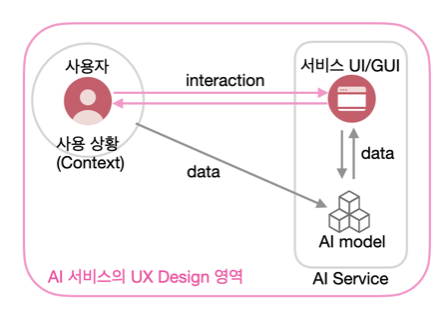
\includegraphics{img/fig1.png}

}

\caption{사용자, AI Service, AI model과 UX Design의 관계 다이어그램}

\end{figure}%

\section{UX 디자인 대상으로서의 AI와 UX 디자인 도구로서의
AI}\label{ux-uxb514uxc790uxc778-uxb300uxc0c1uxc73cuxb85cuxc11cuxc758-aiuxc640-ux-uxb514uxc790uxc778-uxb3c4uxad6cuxb85cuxc11cuxc758-ai}

본 교재의 학습 주제는 데이터 기반 디자인이므로 UX 디자인과 AI의 두가지
연결 지점에서 사용하는 데이터의 특징을 살펴보겠습니다. 첫번째 연결
지점은 인공지능 서비스가 UX 디자인의 대상이 되는 경우, 즉 인공지능
서비스 개발을 위한 UX 디자인을 하는 지점입니다. 이 경우에 디자이너가
다루는 데이터는 인공지능 서비스가 학습하고, 테스트하고, 수집하는 사용자
및 서비스 관련 데이터가 디자인의 대상이 됩니다. 보통 디자이너는 인공지능
서비스 개발에서 사용자가 접하는 화면 그래픽(GUI)이나 인터렉션을
디자인하는 업무에 한정된다고 생각하기 쉽지만, 인공지능 서비스가 어떤
사용자 경험을 수집하고 이해해야 효과적인 서비스가 가능한지를 판단하려면
인공지능 모델 개발의 초기 단계부터 UX 디자이너가 참여해야합니다.

디자이너는 인공지능 모델을 구축할 때 인공지능이 학습할 데이터의 내용과
형식에 대하여 이해하고, 서비스의 환경과 사용자 상황에 맞는 학습 데이터를
선정하는 일에 참여합니다. 또한 인공지능 모델이 구축된 후에 성능을
테스트하고, 서비스의 완성도를 검증하는 일에도 참여해야합니다. 그리고
인공지능 서비스가 제공될 때, 사용자가 서비스와 잘 소통하고, 서비스
내용을 이해할 수 있는 사용자 접점을 디자인해야 합니다. 마지막으로
사용자의 피드백데이터를 기반으로 인공지능 모델과 서비스를 개선할 수 있는
디자인을 제시하여 서비스의 성장을 이끌게 됩니다. 이렇게 UX 디자이너는
인공지능 서비스 개발과 운영, 평가의 전반에 사용자 경험을 반영하여
서비스의 질을 확보하는 중요한 역할을 하고, 이를 위하여 서비스 전체
과정에서 사용되고, 생성되는 데이터에 대한 문해력이 필요하고, 인공지능
모델 개발자, 서비스 개발자 등 기술 전문가와의 협업 능력도 요구됩니다.
마찬가지로, 디자이너와의 효과적인 협업을 위하여 기술 전문가들도 사용자
경험과 디자인을 이해하는 역량이 요구되고 있습니다.

\begin{figure}[H]

{\centering 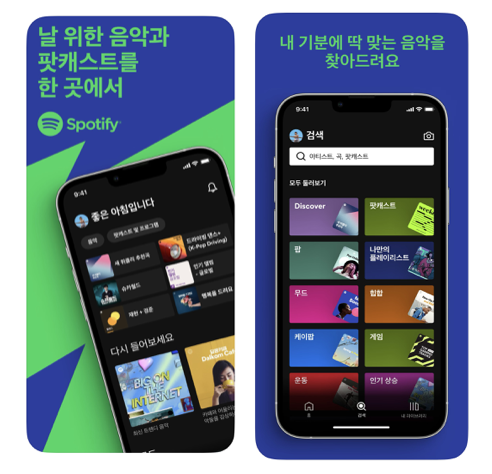
\includegraphics{img/fig2.png}

}

\caption{사용자의 청취 기록을 분석하여 'Discover Weekly'와 같은 맞춤형
콘텐츠를 제공하는 글로벌 음악 스트리밍 서비스, Spotify(3)}

\end{figure}%

두번째, 인공지능은 UX 디자인을 위한 도구 역할을 할 수 있습니다. 데이터
분석과 시각화, 아이디어 도출, 디자인 레이아웃 제안, 그래픽 시안 제작 등
디자인 프로세스의 여러 활동들이 인공지능 기술을 활용한 디자인 서비스로
제공되고 있고, 디자인하는 인공지능 서비스는 앞으로도 영역을 확장하여
발전해 나갈 것입니다. 인공지능 기술을 활용한 디자인 방법은 디자인의
생산성을 높이는 데 크게 기여하고 있습니다. 인공지능 기술은 디자이너의
사고와 작업 방식을 학습하여 디자이너처럼 데이터를 처리하고 그 결과물을
제안합니다. 이러한 상황에서 디자이너들이 기술을 더 잘 활용하고, 디자인의
역량을 확대하기 위해서는 디자인하는 인공지능 기술들이 데이터를 처리하는
방법을 이해하고 활용할 수 있어야하며, 나아가 인공지능이 더 높은 수준의
디자인 작업을 지원할 수 있도록 디자인 데이터와 디자인 행위를 데이터
기술과 연계하는 방법을 개발할 필요가 있습니다.

아래의 기사는 UX 디자인 업무에 AI 서비스를 사용하는 구체적인 업무 내용과
방법들을 설명하고 있습니다. (4)

\href{https://www.nngroup.com/articles/ai-ux-getting-started/}{AI for
UX: Getting Started}

2024년 7월에는 대표적인 UX/UI 표현 도구인 피그마에서 AI 기술을
적극적으로 활용한 디자인과 개발, 프레젠테이션 기능들을 선보였습니다. (5)

\href{https://help.figma.com/hc/ko/articles/24037640924823-Config-2024에서-발표된-새로운-기능}{Config
2024에서 발표된 새로운 기능}

이렇게 UX 디자인에 인공지능 기술이 들어와 디자이너의 업무를 수행하게
된다면 어떤 일들이 벌어질까요? 인공지능이 디자인을 할 수 있으므로
디자이너의 일자리가 없어질까요? 인공지능이 담당할 수 없는 창의적이고,
모험적인 업무에는 소수의 디자이너가 주도하고, 인공지능이 디자이너의
업무를 대신하는 것이 가능한 단순 반복적 디자인 작업이나 패턴화된 디자인
작업은 사람대신 인공지능이 대체하게 될 것입니다. 또 많은 디자이너들은
인공지능에게 할 일을 지시하거나 인공지능의 결과물을 검수하는 일, 그리고
인공지능이 디자인 업무를 할 수 있도록 디자인 업무를 디지털 데이터
중심으로 변환하고, 패턴화하는 일을 하거나, 인공지능에게 학습 데이터를
제공하는 일들을 하게 될 것입니다. 이렇게 인공지능 기반 디자인 도구들은
디자이너의 업무 내용이나 업무 역량의 변화를 이끌고, 디자인 전문가가 아닌
사람들과 디자인 업무의 협업자들이 인공지능 서비스를 활용하여 쉽게 UX
디자인 문제들을 해결하게 할 것으로 예상합니다. 기술은 본래 의식이
없습니다. 기술이 우리에게 긍정적인 역할을 할지, 부정적인 역할을 할지는
인간의 사용 의도에 따라 달라질 수 있습니다. 디자이너는 중립적인 인공지능
기술이 우리에게 유리한 방향으로 기여하도록 잘 이끌어 가야 하겠습니다.

(문헌 3) Spotify(스포티파이), Apple app store

(문헌 4) Kate Moran, Jakob Nielsen, ``AI for UX: Getting Started'',
\url{https://www.nngroup.com/articles/ai-ux-getting-started/}, (2023)

(문헌 5) Figma Learn, ``Config 2024에서 발표된 새로운 기능'',
\url{https://help.figma.com/hc/ko/articles/24037640924823-Config-2024에서-발표된-새로운-기능},
(2024)

\chapter{ch3. 데이터 기반 디자인 (Data Driven
Design)}\label{ch3.-uxb370uxc774uxd130-uxae30uxbc18-uxb514uxc790uxc778-data-driven-design}

데이터 기반 디자인(Data Driven Design)이란 디자인 대상과 관련된 방대한
정량화 데이터를 디자인 설계와 의사 결정의 근거로 활용하는 기법과 정량화
테스트를 통하여 디자인 결과물을 평가, 검증하는 기법을 말합니다.(6) 쉽게
말하면, 데이터에 근거하여 디자인 의사 결정을 수행하는 기법이라고 할 수
있습니다. 데이터 기반 디자인 방법론은 디지털 데이터들을 지속적으로
생산하고 축적하는 웹이나 앱 기반 서비스에 쉽게 적용되기 때문에 구글 등
IT 서비스 기업들이 디지털 서비스의 개발과 운영에 활용하고 있습니다.
현재의 데이터 기반 디자인 연구들은 대부분 인터넷을 통하여 수집된 사용자
로그 데이터를 대상으로 이루어지고 있으나, 점차 사물인터넷(IoT: Internet
of Things) 센서 데이터를 사용하는 등 더 다양한 데이터 자원을 활용하는
방향으로 발전하고 있습니다.

데이터 기반 디자인 서비스 및 컨설팅을 제공하는 산업은 증가 추세에
있으며, 디지털 콘텐츠(웹/앱 서비스)의 사용자 로그 데이터를 시각화하여
사용자 유입 분석, 사용 행태 분석, A/B 테스팅 분석 결과를 제공하는
서비스가 주를 이룹니다. 데이터 기반 디자인을 수행하기 위하여 정량적 통계
분석 및 데이터 시각화 서비스를 지원하는 도구 및 컨설팅 비즈니스 사례에는
구글 애널리틱스(Google Analytics), 태블로(Tableau), 어도비 타깃(Adobe
Target) 서비스 등이 있으며, 각 서비스에 대하여는 다음 단원에서 자세히
다루도록 하겠습니다. (7)

앞서 인공지능 서비스를 디자인하기 위해서는 디자이너가 데이터에 대한
이해가 풍부해야한다고 설명했는데, 선행 연구에 의하면, 인공지능 서비스
개발을 위하여 디자이너는 서비스 및 사용자 관련 데이터를 원격으로 수집할
수 있는 능력과 수집된 데이터에 대한 정량적이고 정성적인 분석과 시각화를
통하여 사용자 행동을 해석하여 디자인에 반영할 수 있는 능력이 요구됩니다.
그리고 실제로 인공지능 서비스를 개발하는 디자이너들은 데이터 중심의 업무
환경에서 데이터의 기초적 통계 분석, 데이터 시각화, A/B 테스팅 기법을
매우 자주 사용하고 있다고 합니다. 그러므로 연구 팀은 디자이너가 데이터로
생각하고, 데이터로 작업하며, 데이터 전문가들과 소통할 수 있도록 하는
교육 과정을 UX 디자인 교육에 반영해야 한다고 주장하고, 또한 UX, HCI
교육에서 디자이너, 데이터 전문가, 엔지니어, 사용자 연구자 등이 함께
협업하는 학제적 수업을 제공하여 학생들이 협업 능력과 창의성을 기를 수
있도록 해야 한다고 제안하였습니다.(8) 선행 연구에서 제시한 바와 같이,
인공지능 서비스를 디자인하기 위한 데이터 문해력은 데이터 기반 디자인을
수행하기 위해 필요한 역량과 일치하고 있습니다. 데이터 기반 디자인을
공부하면서 인공지능 서비스의 디자인 역량을 함께 준비할 수 있다니, 더욱
기대되지 않나요? 그럼 다음 단원 부터는 구체적으로 데이터 기반 디자인의
방법들을 경험해 볼까요?

(문헌 6) Rochelle King, Elizabeth Churchill, and Caitlin Tan,
『Designing with data』, O'reilly, (2017), pp.3-6

(문헌 7) 이현진, 『데이터 드리븐 디자인』, UX리뷰, (2024), pp.43-44

(문헌 8) Qian Yang, Alex Scuito, John Zimmerman, Jodi Forlizzi, and
Aaron Steinfeld, ``Investigating How Experienced UX Designers
Effectively Work with Machine Learning'', DIS(Design Information
Systems)(2018), Hong Kong, pp.585--596

\part{\textbf{part 2. 디자인 리서치를 위한 탐구적 데이터 분석}}

\chapter*{part 2. 디자인 리서치를 위한 탐구적 데이터
분석}\label{part-2.-uxb514uxc790uxc778-uxb9acuxc11cuxce58uxb97c-uxc704uxd55c-uxd0d0uxad6cuxc801-uxb370uxc774uxd130-uxbd84uxc11d-1}
\addcontentsline{toc}{chapter}{part 2. 디자인 리서치를 위한 탐구적
데이터 분석}

\markboth{part 2. 디자인 리서치를 위한 탐구적 데이터 분석}{part 2.
디자인 리서치를 위한 탐구적 데이터 분석}

이번 단원은 데이터 과학의 데이터 분석 방법론인 탐구적 데이터 분석 방법의
개요를 학습하고 탐구적 데이터 분석을 통하여 디자인 리서치를 어떻게
수행하는지의 사례들을 살펴봅니다. 또한 탐구적 데이터 분석 활동을
지원하는 데이터 분석 도구들의 장단점과 실무에서의 사용 현황들을
알아보고, 향후에 다양한 도구들을 사용할 수 있는 기초 소양을 준비합니다.
그리고 3단원 부터 본격적으로 시작되는 데이터 기반 디자인 실습 과제의
기본 방법론인 Lean UX 프로세스의 개념을 공부하여 실습 프로젝트 진행을
위한 기초를 다져보겠습니다.

\href{ch1.\%20디자인\%20리서치와\%20탐구적\%20데이터\%20분석.qmd}{ch1.
디자인 리서치와 탐구적 데이터 분석 (EDA:Exploratory Data Analysis)}

\href{ch2.디자인\%20리서치를\%20위한\%20탐구적\%20데이터\%20분석\%20사례\%20(1).qmd}{ch2.디자인
리서치를 위한 탐구적 데이터 분석 사례 (1): 서울시 미세먼지 측정 데이터
분석 사례}

\href{ch3.디자인\%20리서치를\%20위한\%20탐구적\%20데이터\%20분석\%20사례\%20(2).qmd}{ch3.디자인
리서치를 위한 탐구적 데이터 분석 사례 (2): StudentLife 데이터 분석 사례}

\href{ch4.\%20EDA를\%20위한\%20데이터\%20분석\%20도구들.qmd}{ch4. EDA를
위한 데이터 분석 도구들}

\href{ch5.\%20Lean\%20UX\%20프로세스와\%20데이터\%20기반\%20디자인.qmd}{ch5.
Lean UX 프로세스와 데이터 기반 디자인}

\chapter{ch1. 디자인 리서치와 탐구적 데이터 분석 (EDA:Exploratory Data
Analysis)}\label{ch1.-uxb514uxc790uxc778-uxb9acuxc11cuxce58uxc640-uxd0d0uxad6cuxc801-uxb370uxc774uxd130-uxbd84uxc11d-edaexploratory-data-analysis}

\section{디자인
리서치란}\label{uxb514uxc790uxc778-uxb9acuxc11cuxce58uxb780}

디자인 리서치란 디자이너가 디자인 과정에서 디자인 문제를 이해하고, 주요
의사결정을 하기 위해 여러 관련 데이터를 수집, 분석, 모델링하는 과정을
말합니다. UX 디자인의 특징에 다양한 디자인 리서치 방법론이 포함될 정도로
디자인 리서치는 UX 디자인에서 매우 중요한 과정입니다. 디자인 리서치
대상인 데이터는 보통 사용자와 관련한 데이터, 프로젝트와 관련된 데이터,
그리고 프로젝트에 영향을 주는 시대나 사회, 기술의 변화에 관련한
데이터들이 포함됩니다. 디자이너는 이러한 데이터들을 적절한 방법으로
이해하고 분석하여 디자인 의사결정에 필요한 중간 산출물을 도출합니다.
디자인 리서치 과정을 통하여 디자이너가 만들어내는 중간 산출물 정보는
사용자 조사나 경쟁 제품 분석 보고서, 어피니티 다이어그램, 사용자
페르소나, 사용자 여정 지도, 콘텐츠 정보 구조도, 스토리보드, 서비스
프로토타입 등입니다. 이렇게 생성된 정보들은 디자인 해결안의 방향과
내용을 결정하는 근거가 됩니다. 그러므로 디자인 리서치가 디자인 결과물의
성공을 좌우한다고 볼 수도 있습니다. 결과적으로, 디자인 리서치는 사용자의
만족도를 높이고 비즈니스 목표를 달성하는 데 중요한 역할을 합니다.

\section{탐구적 데이터
분석이란}\label{uxd0d0uxad6cuxc801-uxb370uxc774uxd130-uxbd84uxc11duxc774uxb780}

탐구적 데이터 분석(EDA, Explanatory DataAnalysis)은 데이터 과학의 데이터
분석 방법 중의 하나로, 데이터 시각화 기술을 사용하여 데이터의 특징을
탐지하고 트렌드나 패턴을 확인하여 인사이트를 발견하는 데이터 분석
방법입니다. 탐구적 분석은 데이터 분석의 초기 단계에서 가장 많이
사용되고, 깊은 통찰력을 제공하며 분석 결과를 시각적으로 제시함으로써
비전문가들도 내용을 쉽게 이해할 수 있게 하는 특징이 있습니다. 데이터
분석 소프트웨어 플랫폼 기업인 Posit의 수석 과학자인 해들리 위컴(Hadley
Wichham)은 탐구적 데이터 분석 방법을 통하여 각 변수 별로 일반적인 값과
비정상적인 값의 상태, 변수 간의 상관관계와 구조를 확인할 수 있다고
하였습니다. 그는 저서에서 탐구적 데이터 분석 과정에 대하여 {[}그림
3{]}과 같이 표현했는데, 먼저 데이터를 가져오기 하여(Import) 정리한(Tidy)
뒤, 데이터를 분석에 적합한 형태로 변형하고(Transform), 데이터
시각화(Visualize)와 데이터 모델링(Model)을 반복적으로 수행하여 목표한
분석 결과가 나오면, 분석 내용을 이해하기 좋은 형태로
소통한다고(Communicate) 설명합니다.

\begin{figure}[H]

{\centering 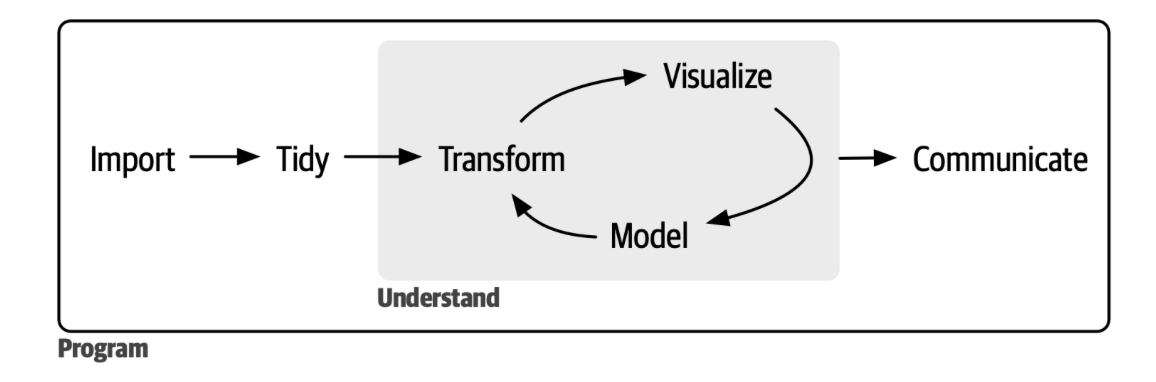
\includegraphics{img/fig3.png}

}

\caption{탐구적 데이터 분석 프로세스 다이어그램(9)}

\end{figure}%

\section{디자인 리서치와 탐구적 데이터 분석의
만남}\label{uxb514uxc790uxc778-uxb9acuxc11cuxce58uxc640-uxd0d0uxad6cuxc801-uxb370uxc774uxd130-uxbd84uxc11duxc758-uxb9ccuxb0a8}

탐구적 분석에서 데이터(문제)의 현황을 탐지하고 트렌드나 패턴을 통하여
인사이트를 발견한다는 것은 더블 다이아몬드 디자인 프로세스 모델의
앞부분인 문제의 발견과 정의 단계에서 하는 활동과 매우 유사한 방법입니다.
다만 디자이너는 이 작업을 다양한 형식(비정형)의 자료를 대상으로 하고
통계 기법을 포함하여 정량, 정성, 직관적인 연구 기법을 다양하게 사용하여
수행하지만, 데이터 과학에서는 대상 데이터 형식을 정제하여 통계적 분석과
통계적 시각화 기법으로 결과를 도출한다는 점이 다릅니다.

그리고 위컴이 제시한 {[}그림 3{]}의 '탐구적 데이터 분석 프로세스
다이어그램'에는 데이터의 탐색이 의미 있는 인사이트를 발견할 때까지
반복적으로 수행되는 속성이 표현되어 있는데, 이는 디자인 프로세스의
반복적 속성과도 상통합니다. 그래서 교재의 데이터 기반 디자인
실습과제에서는 디자인 리서치 과정에서 탐구적 데이터 분석 방법을
적극적으로 활용하여 프로젝트를 진행하고자 합니다. 앞으로의 디자인 리서치
실습 과제에서 데이터 시각화 그래프들을 도출하거나, 이미 공개된 분석
보고서의 그래프들을 수집하여 그래프들의 인사이트를 도출하는 탐구적
데이터 분석 방법을 사용할 예정입니다.

(문헌 9)Hadley Wichham, Garrett. Grolemund, 『R for Data Science(2e.)』,
(2023), \url{https://r4ds.hadley.nz/intro}

\chapter{ch2.디자인 리서치를 위한 탐구적 데이터 분석 사례 (1): 서울시
미세먼지 측정 데이터 분석
사례}\label{ch2.uxb514uxc790uxc778-uxb9acuxc11cuxce58uxb97c-uxc704uxd55c-uxd0d0uxad6cuxc801-uxb370uxc774uxd130-uxbd84uxc11d-uxc0acuxb840-1-uxc11cuxc6b8uxc2dc-uxbbf8uxc138uxba3cuxc9c0-uxce21uxc815-uxb370uxc774uxd130-uxbd84uxc11d-uxc0acuxb840}

앞 장에서 탐구적 데이터 분석 방법을 통하여 각 변수 별로 일반적인 값과
비정상적인 값의 상태, 변수 간의 상관관계와 구조를 확인할 수 있다고
하였습니다. 이번에는 실제 데이터의 탐구적 분석 사례를 통하여 변수와 값의
현황과 패턴을 어떻게 도출하는지 살펴보도록 하겠습니다.

\section{미세먼지 정보 앱 디자인을 위한 미세먼지 데이터 분석 사례
개요}\label{uxbbf8uxc138uxba3cuxc9c0-uxc815uxbcf4-uxc571-uxb514uxc790uxc778uxc744-uxc704uxd55c-uxbbf8uxc138uxba3cuxc9c0-uxb370uxc774uxd130-uxbd84uxc11d-uxc0acuxb840-uxac1cuxc694}

다음의 데이터 분석 사례는 서울의 미세먼지 현황과 예보를 사용자들의 정보
요구에 맞게 안내해주는 앱 서비스를 디자인한다는 가정하에 공공
데이터(Pulblic data)로 공개되어 있는 서울시 미세먼지 측정 데이터를
탐구적 데이터 분석 기법을 사용하여 미세먼지 정보 앱 서비스 디자인을 위한
디자인 인사이트를 도출한 사례입니다. 이 사례는 빅데이터의 탐구적 분석
결과를 어떻게 디자인에 반영할 수 있는지를 연구하고자 제작한 가상
사례입니다.

분석 사례에 사용한 공공 데이터는 다음과 같습니다.

\begin{itemize}
\tightlist
\item
  서울 25개 측정소의 10년간 미세먼지 현황 데이터 (2008-2018년, 10년간의
  측정데이터)
\item
  2018년 서울 25개 구의 시간별 미세먼지 및 기타 오염물질 측정값
\item
  서울시 미세먼지/ 오염물질 측정소의 주소 정보
\item
  2018년 서울기상관측소의 날씨 데이터 (온도, 습도, 풍향)
\end{itemize}

여기에 서비스에 대한 사용자 니즈 관련 정보를 수집하기 위하여 목표
서비스와 비슷한 유사 앱 서비스에 대한 앱스토어의 사용자 평가 데이터
(`미세미세'와 `에어비주얼' 앱의 사용자 평가 데이터)도 분석하였습니다.

이 데이터들을 통하여 서비스의 사용자 니즈를 도출하고, 사용자의 미세먼지
정보 요구를 만족하기 위하여 미세먼지 현황과 미세먼지 예보 정보를 어떻게
제공해야 하는지를 데이터 분석을 통하여 발견하였고, 이 인사이트들을
앱디자인의 콘셉트에 반영하였습니다.

\section{1) 유사 앱 서비스에 대한 앱스토어의 사용자 평가 데이터로 사용자
니즈
발견하기}\label{uxc720uxc0ac-uxc571-uxc11cuxbe44uxc2a4uxc5d0-uxb300uxd55c-uxc571uxc2a4uxd1a0uxc5b4uxc758-uxc0acuxc6a9uxc790-uxd3c9uxac00-uxb370uxc774uxd130uxb85c-uxc0acuxc6a9uxc790-uxb2c8uxc988-uxbc1cuxacacuxd558uxae30}

다음의 {[}표 1{]}은 미세먼지 앱 `미세미세', '에어비주얼'의 앱 스토어
평가 데이터 내용 및 언급 건수입니다. 앱의 디자인은 자주 업데이트 되고,
여러 버전의 디자인 평가가 섞이게 되면 신뢰성이 떨어지므로 연구 시점인
2021년에 운영중인 디자인 버전에 대한 평가 데이터를 수집했습니다. (데이터
수집 기간: 2021.3.1-2021.5.31)

사용자들의 앱 평가 내용을 사용자 정보 데이터와 앱 사용 시점 데이터,
평가에서 언급한 서비스 내용으로 분류하여 앱의 사용자 경험과 관련한 주요
키워드를 도출했습니다.

{[}표 1{]} 미세먼지 앱 `미세미세', '에어비주얼'의 앱 스토어 평가 데이터
내용 및 언급 건수

\begin{longtable}[]{@{}
  >{\raggedright\arraybackslash}p{(\columnwidth - 6\tabcolsep) * \real{0.2083}}
  >{\raggedright\arraybackslash}p{(\columnwidth - 6\tabcolsep) * \real{0.2083}}
  >{\raggedright\arraybackslash}p{(\columnwidth - 6\tabcolsep) * \real{0.2083}}
  >{\raggedright\arraybackslash}p{(\columnwidth - 6\tabcolsep) * \real{0.2083}}@{}}
\toprule\noalign{}
\begin{minipage}[b]{\linewidth}\raggedright
주요 데이터 변수
\end{minipage} & \begin{minipage}[b]{\linewidth}\raggedright
\end{minipage} & \begin{minipage}[b]{\linewidth}\raggedright
미세미세 앱 평가내용 (총 188건 중 언급 건수)
\end{minipage} & \begin{minipage}[b]{\linewidth}\raggedright
에어비주얼 앱 평가내용(총 109건 중 언급건수)
\end{minipage} \\
\midrule\noalign{}
\endhead
\bottomrule\noalign{}
\endlastfoot
사용자 데이터 & 질병 /가족구성 등 & 폐질환(2) &
\begin{minipage}[t]{\linewidth}\raggedright
육아(1)\\
타지역 친척 확인(1)\strut
\end{minipage} \\
사용 상황 데이터 & 사용 시점 등 &
\begin{minipage}[t]{\linewidth}\raggedright
아침(3)\\
외출(1)\\
수시확인(2)\strut
\end{minipage} & \begin{minipage}[t]{\linewidth}\raggedright
해외 정보 확인(3) 운동, 야외활동(1) 아침(2)\\
환기(2)\\
외출(2)\\
수시확인(4)\strut
\end{minipage} \\
서비스 내용 데이터 & 서비스 불만 및 오류 &
\begin{minipage}[t]{\linewidth}\raggedright
접속 오류(9)\\
위젯 불만 / 오류(11)\\
지도표기 오류(11) 시간표기 오류(5)\\
기타(7)\strut
\end{minipage} & \begin{minipage}[t]{\linewidth}\raggedright
위치 표기 오류(5)\\
와치 연동 오류(4) 위젯 오류(3)\\
기타(3)\strut
\end{minipage} \\
& 신뢰성 & \begin{minipage}[t]{\linewidth}\raggedright
신뢰함(16)\\
신뢰성 제기(8)\strut
\end{minipage} & \begin{minipage}[t]{\linewidth}\raggedright
신뢰함(14)\\
신뢰성 제기(1)\strut
\end{minipage} \\
& 앱의 장점 & \begin{minipage}[t]{\linewidth}\raggedright
편리한 디자인(22) 한눈에 보임(9)\\
상세 설명(6)\\
캐릭터 표현(8)\\
알림(4)\strut
\end{minipage} & \begin{minipage}[t]{\linewidth}\raggedright
편리한 디자인(4)\\
한눈에 보임(2)\\
상세 설명(7) 지역 정보(6) 바람 방향 정보(2)\strut
\end{minipage} \\
& 가치평가 (추천 / 감사 등) &
\begin{minipage}[t]{\linewidth}\raggedright
감사(29)\\
좋음(41)\\
잘 사용중(20)\\
추천 / 필수(14)\strut
\end{minipage} & \begin{minipage}[t]{\linewidth}\raggedright
감사(10)\\
좋음(28)\\
잘 사용중(5)\\
추천 / 필수(4)\strut
\end{minipage} \\
\end{longtable}

앱 평가 키워드 분석을 통하여 제공 정보의 신뢰성과 정확성, 요약 설명과
상세 설명이 포함된 정보의 설명성이 중요한 가치라는 것을 발견했고,
신뢰성, 정확성, 설명성을 높이기 위하여 어떻게 정보를 제공해야하는지를
미세먼지 측정 데이터의 탐구적 분석을 통하여 알아보고자 합니다.

\section{2) 서울시 미세먼지 측정 데이터에 대한 탐구적 분석 인사이트
도출}\label{uxc11cuxc6b8uxc2dc-uxbbf8uxc138uxba3cuxc9c0-uxce21uxc815-uxb370uxc774uxd130uxc5d0-uxb300uxd55c-uxd0d0uxad6cuxc801-uxbd84uxc11d-uxc778uxc0acuxc774uxd2b8-uxb3c4uxcd9c}

\begin{itemize}
\tightlist
\item
  변수와 값의 개념
\end{itemize}

변수(Variable)는 데이터를 구성하는 각각의 항목을 의미합니다. 예를 들어,
사람의 키, 몸무게, 나이 등이 변수입니다. 이 데이터를 통해 다양한 정보를
얻을 수 있습니다. 이번에는 서울시 미세먼지 측정 데이터의 변수에 대해
알아보겠습니다. 값 (Value)은 변수가 가질 수 있는 실제 데이터를
의미합니다. 예를 들어, 사람의 키라는 변수의 값은 170cm, 180cm 등이 될 수
있습니다.

{[}표 2{]}를 보면 시간, 측정소 번호, 미세먼지 값, 초미세먼지 값 등의
변수에 2018-01-01 00:00:00, 101, 29, 17 과 같이 한 사례에 측정된 값들이
1행에 할당되어 있습니다. 그리고 각 값은 시간, 숫자, 텍스트 등의 표현
형식을 가지며, 표현 형식에 따라 분석 방법이나 분석 결과가 달라지게
됩니다. 이렇게 변수 별로 동일한 형식의 값을 여러 사례 수집한 데이터를
분석함으로써 우리는 측정 시간과 측정 장소 별 미세먼지 농도의 현황과 같은
유용한 정보를 얻을 수 있습니다.

{[}표 2{]} 서울시 미세먼지 측정 데이터(위)와 날씨 데이터(아래)의 변수 및
값의 형식

\begin{longtable}[]{@{}
  >{\raggedright\arraybackslash}p{(\columnwidth - 12\tabcolsep) * \real{0.1111}}
  >{\raggedright\arraybackslash}p{(\columnwidth - 12\tabcolsep) * \real{0.1111}}
  >{\raggedright\arraybackslash}p{(\columnwidth - 12\tabcolsep) * \real{0.1111}}
  >{\raggedright\arraybackslash}p{(\columnwidth - 12\tabcolsep) * \real{0.1111}}
  >{\raggedright\arraybackslash}p{(\columnwidth - 12\tabcolsep) * \real{0.1111}}
  >{\raggedright\arraybackslash}p{(\columnwidth - 12\tabcolsep) * \real{0.1111}}
  >{\raggedright\arraybackslash}p{(\columnwidth - 12\tabcolsep) * \real{0.1111}}@{}}
\toprule\noalign{}
\begin{minipage}[b]{\linewidth}\raggedright
시간 ( 월,일 , 시간)
\end{minipage} & \begin{minipage}[b]{\linewidth}\raggedright
측 정소 번호
\end{minipage} & \begin{minipage}[b]{\linewidth}\raggedright
미 세 먼지 값 ( 10pm)
\end{minipage} & \begin{minipage}[b]{\linewidth}\raggedright
초미 세 먼지 값 ( 2 .5pm)
\end{minipage} & \begin{minipage}[b]{\linewidth}\raggedright
월 (달)
\end{minipage} & \begin{minipage}[b]{\linewidth}\raggedright
시 간 (시)
\end{minipage} & \begin{minipage}[b]{\linewidth}\raggedright
측 정소 위 치 (구)
\end{minipage} \\
\midrule\noalign{}
\endhead
\bottomrule\noalign{}
\endlastfoot
\begin{minipage}[t]{\linewidth}\raggedright
2018- 0 1-01\\
00 : 00:00\strut
\end{minipage} & 101 & 29 & 17 & 1 & 0 & 종 로구 \\
\end{longtable}

서울 25개 측정소의 2018년 미세먼지 데이터 : 209,785개의 측정값 (서울
25개 측정소의 2008\textasciitilde2018년 10년간 미세먼지 데이터 :
2,150,195개의 측정값도 같은 형식임.)

\begin{longtable}[]{@{}
  >{\raggedright\arraybackslash}p{(\columnwidth - 10\tabcolsep) * \real{0.1250}}
  >{\raggedright\arraybackslash}p{(\columnwidth - 10\tabcolsep) * \real{0.1250}}
  >{\raggedright\arraybackslash}p{(\columnwidth - 10\tabcolsep) * \real{0.1250}}
  >{\raggedright\arraybackslash}p{(\columnwidth - 10\tabcolsep) * \real{0.1250}}
  >{\raggedright\arraybackslash}p{(\columnwidth - 10\tabcolsep) * \real{0.1250}}
  >{\raggedright\arraybackslash}p{(\columnwidth - 10\tabcolsep) * \real{0.1250}}@{}}
\toprule\noalign{}
\begin{minipage}[b]{\linewidth}\raggedright
시간 (월, 일 ,시간)
\end{minipage} & \begin{minipage}[b]{\linewidth}\raggedright
기온
\end{minipage} & \begin{minipage}[b]{\linewidth}\raggedright
풍속
\end{minipage} & \begin{minipage}[b]{\linewidth}\raggedright
풍향
\end{minipage} & \begin{minipage}[b]{\linewidth}\raggedright
습도
\end{minipage} & \begin{minipage}[b]{\linewidth}\raggedright
풍 향이름
\end{minipage} \\
\midrule\noalign{}
\endhead
\bottomrule\noalign{}
\endlastfoot
\begin{minipage}[t]{\linewidth}\raggedright
\section{201 8}\label{section}

01-01\\
0 0 :00:00\strut
\end{minipage} & -3.2 & 0.5 & 110 & 40 & 동남동 \\
\end{longtable}

서울 기상 관측소 (108번 측정소)의 2018년 날씨 데이터 : 8,740개의 측정값

\begin{itemize}
\tightlist
\item
  1년 간의 시간 변화에 따른 미세먼지량의 변화를 선 그래프로 표현한
  데이터 시각화 사례
\end{itemize}

{[}표 2{]}의 시간 변수와 미세먼지 값, 초미세먼지 값 변수에 대한 값의
변화를 그래프로 시각화하면 다음과 같습니다. 이 그래프를 보고 전체적으로
x축의 4월, 12월 주변 구간에서 측정량이 높게 나타나고, 여름에는
미세먼지량이 적게 나타나고 있어 미세먼지 측정량은 계절 차이가 있다고 할
수 있습니다. 전체적으로 미세먼지(빨강) 그래프가 위쪽에 자리하여 측정량이
많고, 측정량의 변동 폭도 큼을 볼 수 있습니다. 매우 높은 수치를 보여주는
지점들도 미세먼지 측정량(빨강)입니다. 그에 비하여 초미세먼지(파랑)는
변동이 작고 고르게 발생하고 있는 현황을 발견할 수 있습니다.

\begin{figure}[H]

{\centering 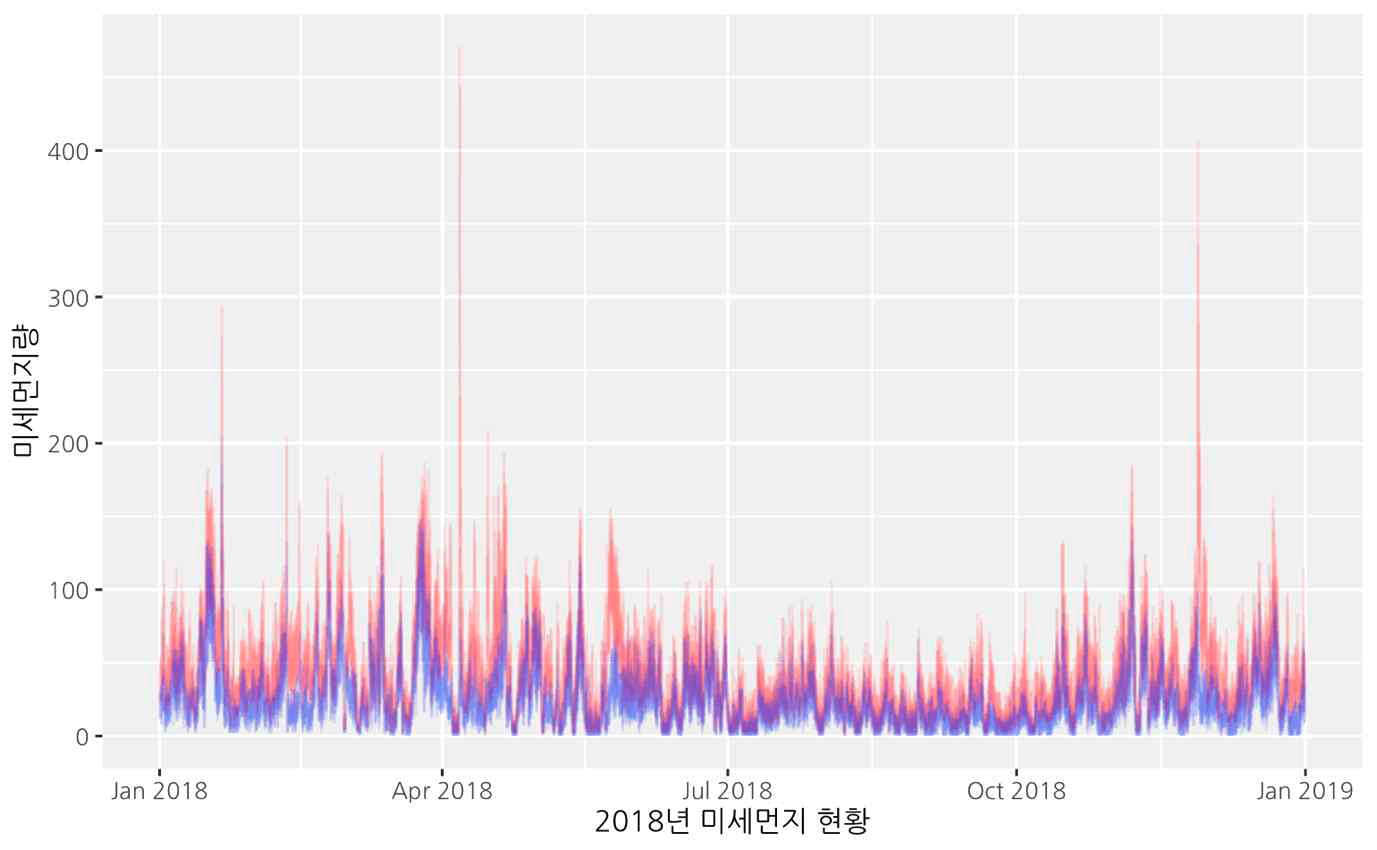
\includegraphics{img/fig4.png}

}

\caption{2018년 서울시 미세먼지(적색)와 초미세먼지(청색)량의 측정값
현황}

\end{figure}%

\begin{itemize}
\tightlist
\item
  2018년 1-5월의 월별 일간 미세먼지 측정량 변화폭을 표현한 데이터 시각화
  그래프 사례
\end{itemize}

아래 그림은 미세먼지가 검출량이 높은 1\textasciitilde5월의 각 월별로
매일의 미세먼지 검출량의 범위가 드러나도록 한 그래프입니다. 막대 처럼
보이는 그래프 부분은 실제는 막대가 아니고 하루 동안의 미세먼지 측정량을
점으로 표현한 것이 모여서 막대처럼 보이고 있습니다. 시간 데이터 값을 월,
일로 분리하면 개별 하루의 측정 변화를 알아볼 수 있습니다. 이 그래프에서
4월 6일의 측정량 변화가 매우 큼을 확인하고, 4월 6일의 시간 별 측정
데이터를 시각화 하게 되었습니다.

\begin{figure}[H]

{\centering 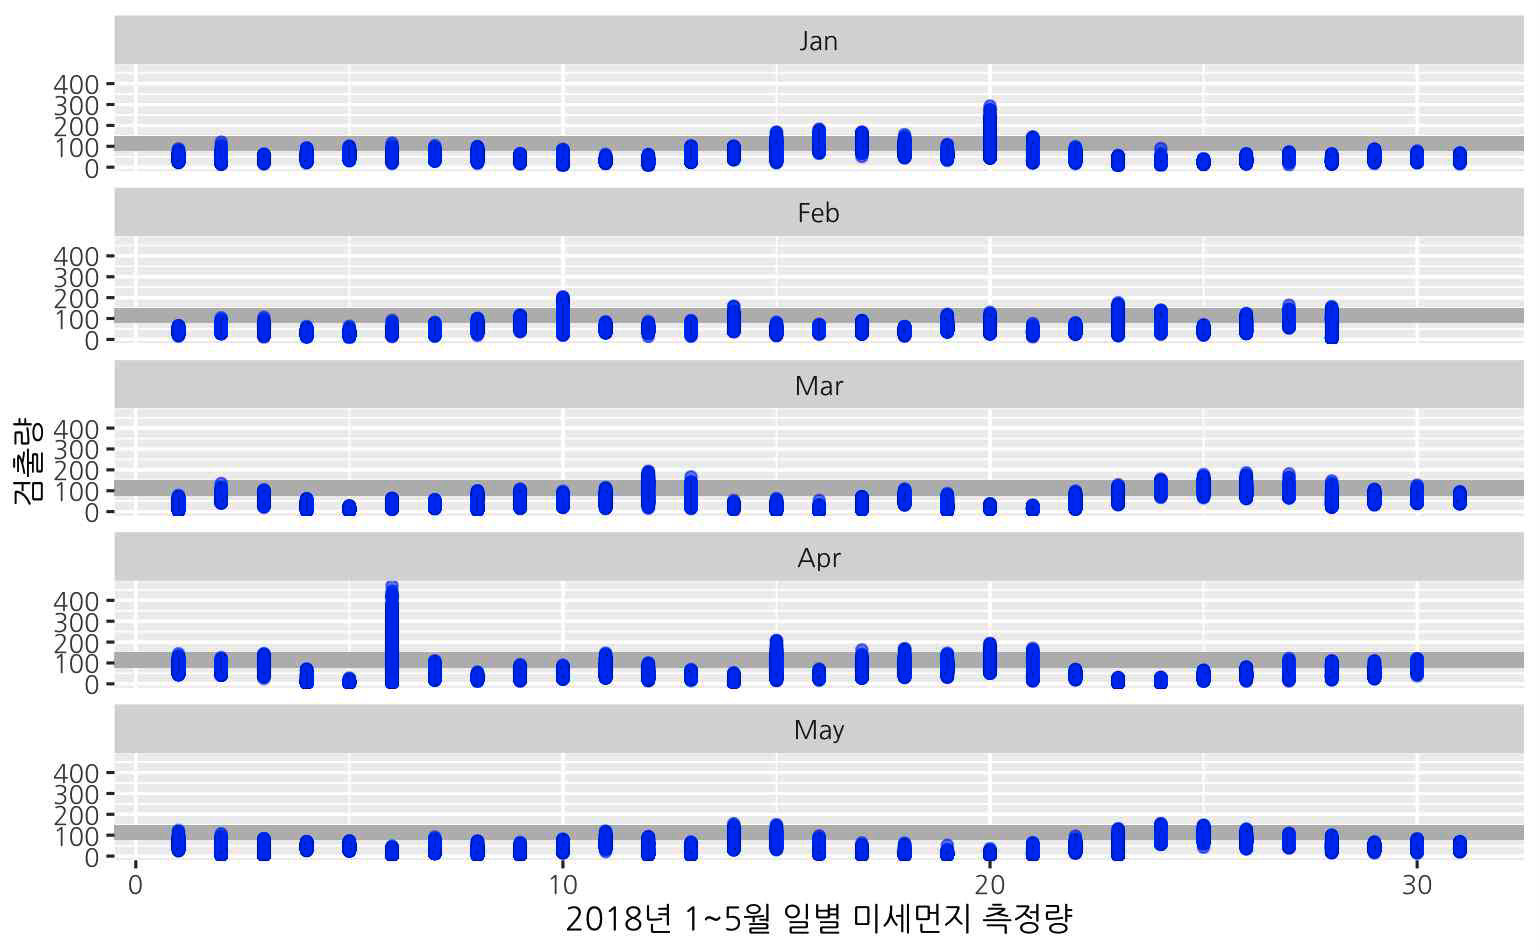
\includegraphics{img/fig5.png}

}

\caption{2018년 상반기(1-5월) 일별 미세먼지 측정량:미세먼지 시즌의 일별
측정량 변화를 보여준다. (회색 영역은 한국환경공단 기준 `미세먼지 나쁨'
단계 범위}

\end{figure}%

\begin{itemize}
\tightlist
\item
  2018년 4월 6일 하루 동안의 서울시 지역구별 미세먼지 측정량의 시각화
  그래프 사례
\end{itemize}

4월 6일의 미세먼지는 일간 변화량이 크고, 매우 나쁨 단계의 수치가 특정
시간대(오전 10시경\textasciitilde 오후11시경)에 집중되어 있습니다. 시간
별 측정량 차이가 크므로 미세먼지 대표값을 표현할 때 일평균 값을 쓰면
안된다는 것을 알 수 있습니다. 그리고 측정량을 꺾은선으로 표현할 때 점차
높아졌다가 낮아지는 흐름이 발견되므로 시간을 구간으로 나누어 측정량 예측
공지를 할 수 있을 것입니다.

측정소 지역별(구별) 특징을 보면 측정량을 다르지만, 시간별 측정 패턴이
다르지는 않아서 측정량의 흐름이 지역별로 동일하게 유지되고 있습니다.
매우 나쁨 단계의 측정량 범위(회색 영역 위쪽)가 너무 넓고, 같은 단계
안에서 측정량에 큰 차이가 존재합니다. 너무 넓은 변화 범위가 같은 단계로
표현되므로 매우 나쁨 단계를 더 나누어 세분화 표기할 필요가 있습니다.

\begin{figure}[H]

{\centering 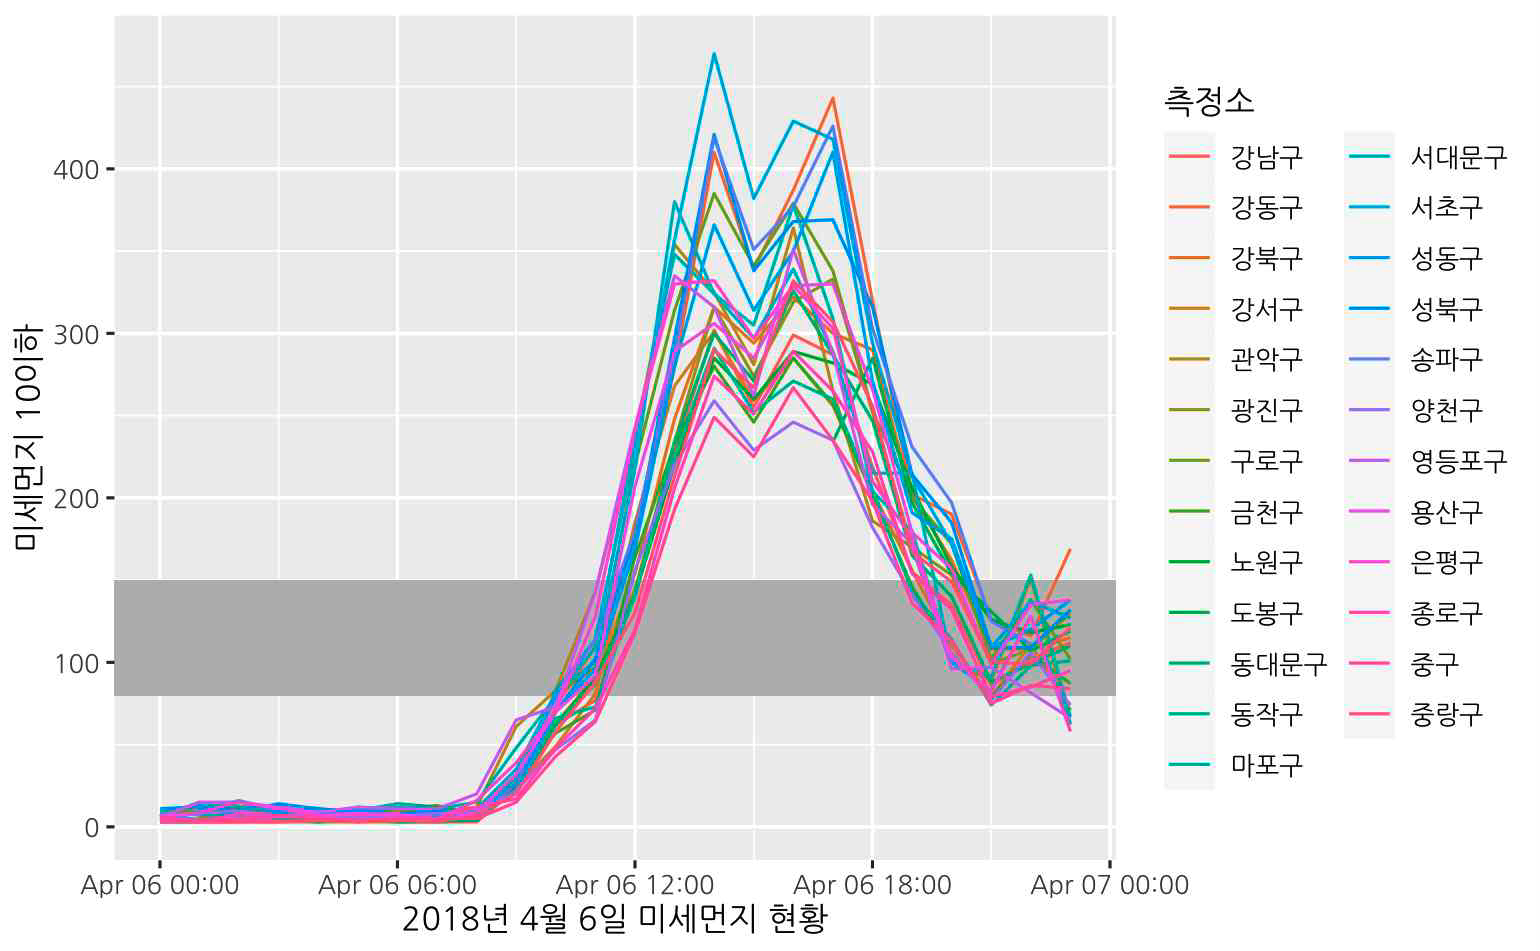
\includegraphics{img/fig6.png}

}

\caption{2018년 4월 6일(년간 미세먼지가 가장 심했던 날)의 시간별,
구별(지역별) 미세먼지 측정 현황(회색 영역은 한국환경공단 기준 `미세먼지
나쁨' 범위)}

\end{figure}%

\begin{itemize}
\tightlist
\item
  서울시 지역구별 미세먼지 아주 나쁨 값이 관측된 횟수 비교 시각화 사례
\end{itemize}

아래 그림은 미세먼지 아주 나쁨 단계 값이 측정된 횟수를 비교한 막대
그래프입니다. 몇 개 지역은 미세먼지 아주 나쁨 상태가 더 자주 발생하고
있음을 알 수 있고, 지역별로 횟수 차이가 존재합니다. 그러므로 특정 지역에
거주하거나 방문하는 경우에는 좀 더 적극적으로 미세먼지 상황 정보를
제공할 필요가 있어 보입니다.

\begin{figure}[H]

{\centering 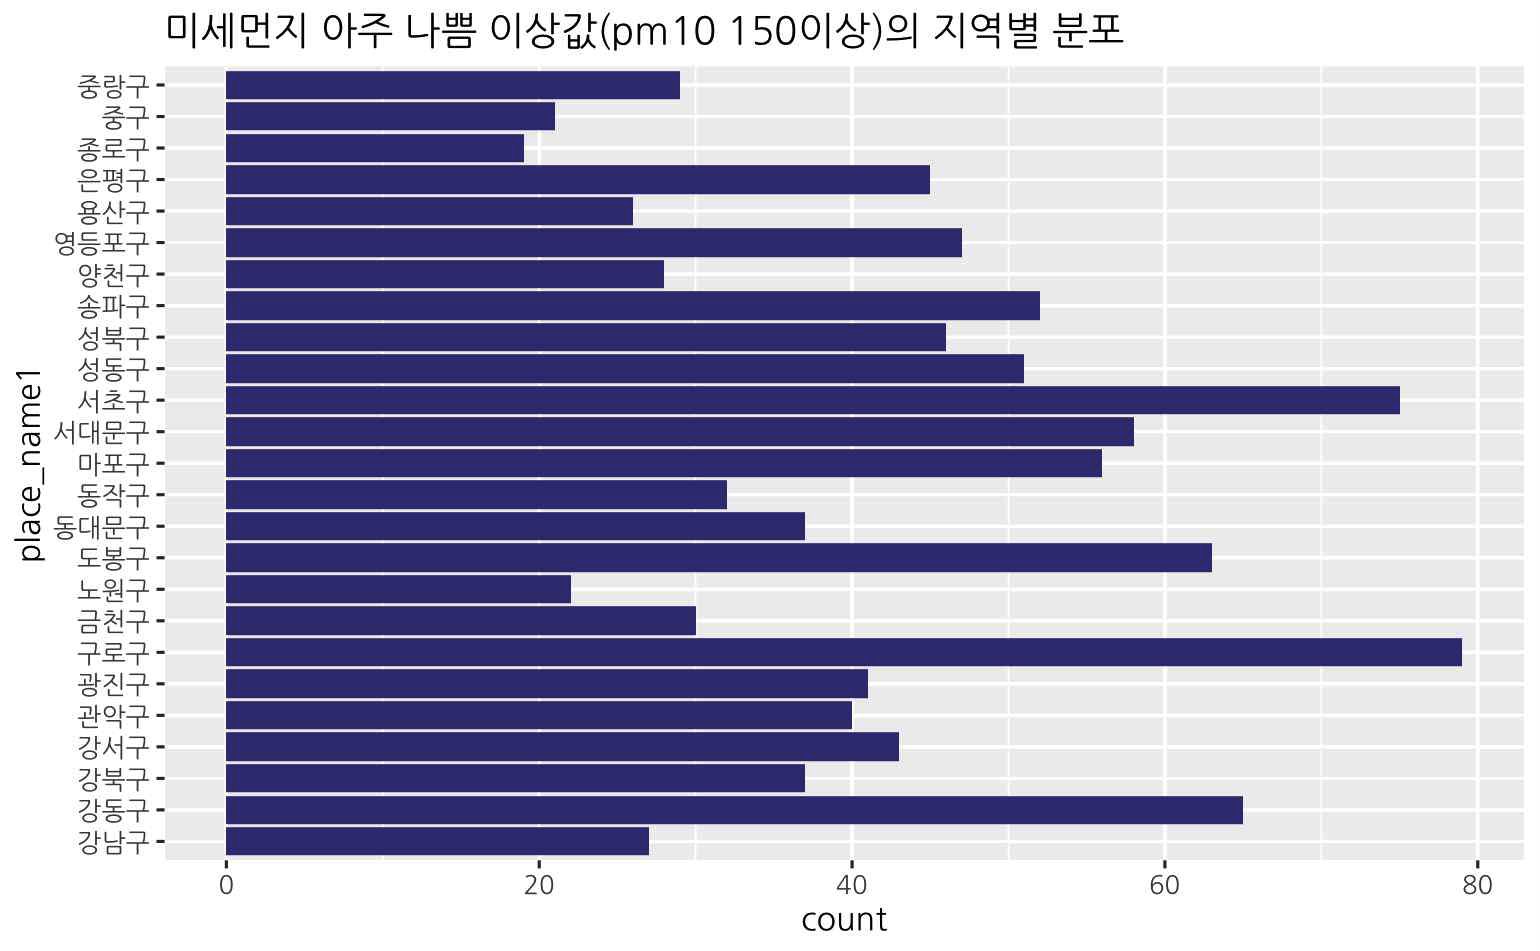
\includegraphics{img/fig7.png}

}

\caption{2018년 서울시 지역구별 미세먼지 `아주 나쁨' 기준 이상 값이
측정된 횟수}

\end{figure}%

본 사례에서는 예시와 같이 다양한 변수 별, 변수 간 데이터 시각화 실험을
통하여 25건의 미세먼지와 초미세먼지 관련 변수들의 현황과 관계 패턴 및
인사이트들을 발견할 수 있었습니다. 탐구적 데이터 분석 작업의 특징은
데이터의 변수 별, 변수 간 시각화를 순차적으로 해보고, 의미 해석을 한 뒤,
그 다음에 어떤 시각화를 진행할지를 작업 과정 중에 판단하고, 앞선
분석에서 제기된 질문에 대한 답을 구하면서 단계적으로 진행하는 특징이
있습니다. 데이터 분석의 순차적이고, 가변적인 작업 과정은 디자인 리서치의
방법에서도 공통적으로 발견되는 특징입니다.

\subsection{3) 미세먼지 측정 데이터의 변수 현황 및 디자인
인사이트}\label{uxbbf8uxc138uxba3cuxc9c0-uxce21uxc815-uxb370uxc774uxd130uxc758-uxbcc0uxc218-uxd604uxd669-uxbc0f-uxb514uxc790uxc778-uxc778uxc0acuxc774uxd2b8}

{[}표 3{]}은 탐구적 데이터 분석을 통하여 발견한 서울시 미세먼지,
초미세먼지 데이터의 현황을 목록화하고, 각 결과를 바탕으로 디자인
인사이트를 도출한 사례입니다. 디자인 인사이트를 도출할 때는 1)의 사용자
니즈 발견에서 도출한 정보의 신뢰성, 정확성, 설명성 키워드를 연계하여
아이디어를 개발합니다.

{[}표 3{]} 미세먼지 및 초미세먼지 측정 데이터의 질문 사항과 분석 결과 및
데이터 패턴을 반영한 디자인 인사이트

\begin{longtable}[]{@{}
  >{\raggedright\arraybackslash}p{(\columnwidth - 4\tabcolsep) * \real{0.2639}}
  >{\raggedright\arraybackslash}p{(\columnwidth - 4\tabcolsep) * \real{0.3333}}
  >{\raggedright\arraybackslash}p{(\columnwidth - 4\tabcolsep) * \real{0.3333}}@{}}
\toprule\noalign{}
\begin{minipage}[b]{\linewidth}\raggedright
주요 변수관련 데이터의 질문 사항: 신뢰성, 데이터 제공 시점 ( 년
,월,일,시간)별 현황, 정보 설명성(요약, 상세(날씨, 지역)
\end{minipage} & \begin{minipage}[b]{\linewidth}\raggedright
분석 결과: 변수 별 값의 현황과 변수 간 상관관계
\end{minipage} & \begin{minipage}[b]{\linewidth}\raggedright
데이터 변수 패턴을 반영하는 디자인 인사이트
\end{minipage} \\
\midrule\noalign{}
\endhead
\bottomrule\noalign{}
\endlastfoot
미세먼지량과 초미세먼지량은 서로 어떤 관계가 있는가. & 대체로 양의
상관관계에 있으나 기준값 이상의 초미세먼지가 기준값 이상의 미세먼지 보다
훨씬 자주 발생한다. & 미세먼지와 초미세먼지 데이터 패턴이 다르므로
내용을 따로 표현하고, 각 패턴에 맞는 표현 방법을 사용한다. \\
년간 미세먼지와 초미세먼지 현황은 어떤 특징을 가지나? & 각 해의
상반기(4월)까지 먼지 발생이 높고, 5-10월까지는 발생량이 낮다가 11월부터
높아진다. 초미세먼지도 같은 패턴을 보이며, 일별 변동이 크다. & 월별
미세먼지 발생 시즌에 따라 다른 표현으로 안내하는 정보 서비스가 필요하다.
발생량이 낮은 기간에는 앱 사용도가 낮을 것이다. \\
월간 미세먼지와 초미세먼지 현황은 어떤 특징을 가지나? & 월 별 차이가
크다. 초미세먼지도 상반기가 많으나, 월별 먼지량의 차이가 상대적으로
작다. & 초미세먼지 정보는 연중 중요도가 지속적으로 높고, 대부분 나쁨
기준량을 초과하여 경각심을 줄 필요가 있다. \\
미세먼지의 시간별 변화에 어떤 패턴이 있는가? & 미세먼지가 많은 날은 특정
시간 대에 먼지량이 집중되며, 아주 나쁨 수준에 매우 큰 편차가 존재한다.
기준 값보다 3-4배 많은 날도 있다. & 현재의 환경 공단 기준 4단계 경보는
아주 나쁨 단계의 심각성을 반영하지 못한다. 단계 구간의 변경이
필요하다. \\
초미세먼지의 시간 별 변화에 어떤 패턴이 있는가? & 초미세먼지가 많은 날은
특정 시간대에 먼지량이 집중되나 편차가 적다. & 시간별 측정량을 강조하되,
일별 정보도 의미있게 다룬다. \\
한국환경공단의 미세먼지 측정 단계는 어떤 의미가 있나? & 4단계로
되어있는데, 시간별 변동이 크므로 하루 측정값의 평균을 사용하는 표준 단계
값은 정확하지 않다. & 정확한 정보 전달을 위해 미세먼지 측정 단계 값을
일별 국내 표준이 아닌 더 정확한 단계로 제공해야 한다.(기존 앱도 더
상세한 국제 기준을 사용함) \\
미세먼지, 초미세먼지와 날씨는 어떤 관계가 있나? 어떤 날씨 정보가 영향을
주나? & 기온, 습도, 풍속은 크게 관련이 없고, 서, 북향의 풍향이 많은 때에
미세먼지, 초미세먼지 발생 빈도가 높다. 풍향은 계절(달)별 먼지 발생에
영향을 미친다. & 풍향 정보가 미세먼지 발생과 연계되므로, 다른 날씨
정보보다 풍향 정보를 잘 연계하여 표현해야 한다. \\
지역(측정소)별 미세먼지, 초미세먼지의 분포는 어떠한가? 지역별 차별화
표현이 필요한가? & 서울시의 구별 미세먼지 발생 패턴은 유사하다. 다만
특히 미세먼지 나쁨 단계 이상 빈도가 큰 지역이 존재한다. & 지역별로 표현
방식이 다를 필요는 없다. 그러나 발생 빈도가 높은 지역에 대한 경고 및
지역별 사용자 옵션으로 더 자세한 미세먼지 정보를 제공할 수 있다. \\
\end{longtable}

\subsection{4) 데이터 변수 패턴 기반의 디자인 컨셉
도출}\label{uxb370uxc774uxd130-uxbcc0uxc218-uxd328uxd134-uxae30uxbc18uxc758-uxb514uxc790uxc778-uxcee8uxc149-uxb3c4uxcd9c}

{[}표 4{]}는 프로젝트 데이터의 주요 변수와 키워드 별 변수 패턴을 반영한
디자인 콘셉트 제안 예시입니다. 앱 서비스에서 제공하는 정보 내용과 정보
제공 방법을 변수 패턴이 반영된 정보 표현 방법으로 제시하였습니다. 이러한
정보 표현 방법을 앱의 화면 레이아웃과 GUI에 반영하여 디자인 해결안을
완성하면, 탐구적 데이터 분석 기법을 디자인 리서치에 사용한 디자인
해결안이 됩니다.

{[}표 4{]} 프로젝트 데이터의 주요 변수와 키워드 별 변수 패턴을 반영한
디자인 콘셉트 제안 예시

\begin{longtable}[]{@{}
  >{\raggedright\arraybackslash}p{(\columnwidth - 6\tabcolsep) * \real{0.1944}}
  >{\raggedright\arraybackslash}p{(\columnwidth - 6\tabcolsep) * \real{0.1944}}
  >{\raggedright\arraybackslash}p{(\columnwidth - 6\tabcolsep) * \real{0.1944}}
  >{\raggedright\arraybackslash}p{(\columnwidth - 6\tabcolsep) * \real{0.3611}}@{}}
\toprule\noalign{}
\begin{minipage}[b]{\linewidth}\raggedright
주요 데이터 변수
\end{minipage} & \begin{minipage}[b]{\linewidth}\raggedright
변수 관련 키워드
\end{minipage} & \begin{minipage}[b]{\linewidth}\raggedright
주요 변수 패턴과 인사이트
\end{minipage} & \begin{minipage}[b]{\linewidth}\raggedright
변수 패턴을 반영한 디자인 콘셉트
\end{minipage} \\
\midrule\noalign{}
\endhead
\bottomrule\noalign{}
\endlastfoot
사용자 데이터 & 질병/ 가족 구성 등 & 특정 사용자 집단별 서비스 니즈와
상관 없이 서비스를 자주 사용하는 사용자의 필요 반영 & \textless 서비스를
자주 사용하는 사용 자\textgreater 서비스를 자주 사용하는(일별 사용 및
수시 사용) 일반 사용자를 타겟으로함. \\
사용자 상황 데이터 & 사용 시점과 빈도, 환경(날씨, 지역) & 매일 및 수시
확인 시점 별 정보 니즈 반영 환경 정보는 지역 상황에 따라 필요성이 다름
날씨는 풍향만 미세먼지에 영향있음. & \textless 매일 확인\textgreater{}
일별 통합 예측시 시간대별 예측 정보 제공 \textless 수시
확인\textgreater{} 측정 시점(시간별) 정보, 1-3시간 후 추이 정보 강조
사용자 선택 옵션으로 지역별 날씨, 미세먼지 상세 정보 제공 \\
서비스 내용 데이터 (서비스 가치) & 정 보의신뢰성/ 정확성 확보 & 년간 시
즌 /월별/일별/ 시간별 발생 패턴이 다름 & \textless 미세먼지 시즌 별 정보
표현 차별화\textgreater{} 미세먼지 집중 기간 (11월-5월)과 그 외 기간의
정보 표현 차별화 여름 및 가을 (6-10월)에는 미세먼지 정보 외 부가 생활
정보 제공 시간별 측정량 중심의 정보 표현 \\
& 정보 설명성 (요약, 상세 설명) & 미세/초미세 먼지의 데이터 특징이 다름
일별 요약은 대표값으로 부적절함 미세먼지의 경우 아주 나쁨 단계 범위가
너무 넓음 & \textless 요약 설명\textgreater{} 미세, 초미세먼지의 표현
방법 차별화 미세 먼지의 아주 나쁨 단계 세분화 (초미세먼지는 그대로 사용)
아주 나쁨 단계의 경각심 표현 강화 \textless 상세 설명\textgreater{}
시간별 정보 중심으로 설명 사용자 옵션으로 사용자 요구에 따른 상세 설명
방법, 알림 방법 제공 \\
& 관심 부가 서비스 & 알림, 위젯 등에서 요약 정보 요구 & \textless 정보
상황에 의한 알림/위젯 디자인\textgreater{} 나쁨 빈도 높은 지역에는 알림
방법 강화 시간별 알림 및 관심 지역 중심의 알림, 위젯 디자인 제공 \\
\end{longtable}

이렇게 디자인 리서치에서 데이터 분석 기법을 사용하면, 적은 노력으로
다량, 장기간의 데이터를 수집 분석하는 것이 가능하여 디자인 리서치의
생산성이 높아집니다. 탐구적 데이터 분석 방법은 대규모이거나 분야간
협업이 중요한 프로젝트에서도 소통 효율을 높이는 데 기여합니다.(7)

또한 이 사례와 같이 사용자에 대한 질적 연구 방법으로는 알 수 없는 콘텐츠
데이터(미세먼지 데이터)의 특징(신뢰성, 정확성, 설명성에 영향을 미치는
정보 속성들)을 데이터 분석 기법을 통하여 발견하고, 이를 디자인 콘셉트로
개발 할 수 있습니다. 이렇게 개발한 콘셉트로 디자인을 완성한 뒤에는 과연
이 디자인이 우리가 개선하고자 한 속성들(신뢰성, 정확성, 설명성)을
개선하였는지 검증해 볼 필요가 있겠죠. 이 검증 과정이 교재의 후반부에서
학습할 A/B 테스팅 입니다.

(문헌 7) 이현진, 『데이터 드리븐 디자인』, UX리뷰, (2024), pp.100-143

\chapter{ch3.디자인 리서치를 위한 탐구적 데이터 분석 사례 (2):
StudentLife 데이터 분석
사례}\label{ch3.uxb514uxc790uxc778-uxb9acuxc11cuxce58uxb97c-uxc704uxd55c-uxd0d0uxad6cuxc801-uxb370uxc774uxd130-uxbd84uxc11d-uxc0acuxb840-2-studentlife-uxb370uxc774uxd130-uxbd84uxc11d-uxc0acuxb840}

\section{StudentLife 데이터 분석 사례
개요}\label{studentlife-uxb370uxc774uxd130-uxbd84uxc11d-uxc0acuxb840-uxac1cuxc694}

StudentLife 연구는 2013년부터 2022년까지 다트머스 대학에서 스마트폰과
웨어러블 기기를 활용하여 학생들의 정신 건강과 행동 데이터를 분석한 장기
프로젝트입니다. 연구팀은 참여 학생들에게 스마트폰 앱을 설치하고,
스마트폰 센서를 활용하여 일상 활동, 위치, 수면 패턴, 통화 기록, 문자
메시지 등을 자동으로 수집하였고, 정기 설문 조사를 실시하였습니다. 이
데이터를 통해 학생들의 스트레스, 우울증, 불안 등의 정신 건강 상태를
평가하고, 학생 활동과 학업 성취도와의 관계를 분석했습니다. 이 연구는
장기간 수집된 데이터를 통해 학생들의 행동 변화와 정신 건강 상태를
심층적으로 연구하며, 이를 바탕으로 학생 지원 방안을 모색하였고, 스마트폰
센서 데이터를 분석하는 방법과 사례에 대한 다수의 논문을 발표하였고,
연구에서 수집한 데이터를 Kaggle 사이트에 공개하였습니다. (10)(11)

프로젝트 기간 변 주요 연구 내용은 다음과 같습니다.

\begin{itemize}
\tightlist
\item
  2013년: 48명의 학생을 대상으로 10주 동안 스마트폰 센서를 통해
  스트레스, 외로움, 수면 패턴 등을 분석하고, 학업 성취도(GPA)와 정신
  건강의 관계를 연구.
\item
  2016년: 83명의 학생을 대상으로 두 학기 동안 스마트폰과 웨어러블 기기를
  이용해 우울증과 불안의 상태를 조사.
\item
  2018년\textasciitilde2022년: 200명의 학생을 대상으로 COVID-19 팬데믹
  기간 포함하여 4년 동안 장기 연구를 수행하고 학생들의 정신 건강과 행동
  변화 분석.
\end{itemize}

\href{https://studentlife.cs.dartmouth.edu}{StudentLife Study}

\href{https://www.kaggle.com/datasets/subigyanepal/college-experience-dataset?resource=download}{College
Experience Study Dataset}

다음의 데이터 시각화 사례들은 본 연구에서 발표한 논문들에서 발췌한
그래프들로 여러 유형의 시각화 그래프와 그래프 해석 사례를 보여주고
있습니다. 이와같이 이미 데이터의 시각화된 분석 자료가 있는 경우, 그래프
해석을 통하여 디자인에 필요한 인사이트를 도출할 수 있습니다. 21년도에
진행한 수업에서는 아래의 그래프들을 해석하여 대학생의 행동 패턴들을
발견하고, 긍정적인 행동 패턴으로의 변화를 유도할 수 있는 모바일 서비스의
디자인 제안을 수업 프로젝트로 진행하였습니다.

다양한 유형의 데이터 시각화 그래프 해석 연습이라고 생각하고 아래에
제시한 사례 그래프들을 읽고 의미를 해석해 봅시다.

\section{1) 실험 참여 대학생의 학기중 생활 패턴
분석}\label{uxc2e4uxd5d8-uxcc38uxc5ec-uxb300uxd559uxc0dduxc758-uxd559uxae30uxc911-uxc0dduxd65c-uxd328uxd134-uxbd84uxc11d}

\begin{figure}[H]

{\centering 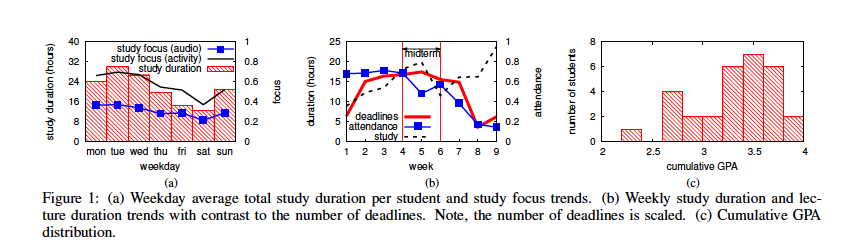
\includegraphics{img/fig8.png}

}

\caption{학생들의 요일(a), 학기 주차 별(b) 공부시간 패턴 변화와 학생
학점 그래프(c)(12)}

\end{figure}%

이 그래프들은 주간 요일 및 학기중 주차 별 학생들의 학업 관련 활동과
학점(GPA)을 시각화한 것입니다. 학업 활동의 변동과 학생들의 성취도를
파악함으로써, 보다 효과적인 학습 전략과 지원 프로그램을 개발하는데에
도움을 줄 수 있습니다.

\begin{itemize}
\item
  그래프 (a): 주중 평균 총 공부 시간 및 공부 집중도 추세

  X축의 요일 별로 Y축의 공부 시간 (그래프 왼쪽 축, 시간) 및 집중도
  (그래프 오른쪽 축, 0\textasciitilde1 사이의 값)를 빨간색 막대그래프:
  각 요일의 공부 시간 (study duration), 파란색 꺾은선 그래프: 오디오
  데이터를 통한 공부 집중도 (study focus (audio)), 검정색 꺽은선 그래프:
  활동 데이터를 통한 공부 집중도 (study focus (activity))로
  표현했습니다. 월요일부터 금요일에는 공부 시간과 집중도가 모두
  높습니다. 특히 주 초반에는 공부 시간이 최대치에 도달합니다. 주말에는
  공부 시간이 급격히 감소합니다. 특히 토요일에 가장 낮은 공부 시간을
  보이며, 일요일에는 약간 증가함을 알 수 있습니다.
\item
  그래프 (b): 학기 주차 별 공부 시간 및 강의 출석 시간과 과제 마감 갯수
  추세

  X축의 주차 별로(1\textasciitilde9주차까지) Y축의 공부 시간 (그래프
  왼쪽 축, 시간) 및 과제 마감 갯수 (그래프 오른쪽 축,
  0\textasciitilde1의 상대 값)를 파란색 꺾은선 그래프: 주간 출석 시간,
  빨간색 꺾은선 그래프: 주간 공부 시간, 검은색 점선 그래프: 마감 갯수로
  표현했습니다. 초기 주차 (1\textasciitilde3주차)는 공부 시간과 출석
  시간이 비교적 안정적으로 유지됩니다. 마감일 수는 적습니다. 중간고사
  기간은(4\textasciitilde6주차) 공부 시간이 급격히 증가하며, 출석 시간도
  증가합니다. 마감일 수도 증가하여 학생들이 중간고사 준비에 몰두하는
  것을 알 수 있습니다. 후기 주차 (7\textasciitilde9주차)는 공부 시간과
  출석 시간이 급격히 감소합니다. 마감일 수도 감소하여 학생들이 학기 말에
  학업 활동이 줄어드는 경향을 보입니다.
\item
  그래프 (c): 누적 GPA (모든 수강 과목의 학점 평균) 분포

  X축은 학점(GPA), Y축은 학생 수를 표현합니다. 대부분의 학생들이 3.0에서
  3.5 사이의 GPA를 가지고 있습니다. 이는 평균 이상의 학업 성취도를
  나타냅니다. 2.5 이하의 GPA를 가진 학생은 비교적 적습니다. 이는 실험에
  참여한 학생들의 전반적인 학업 성취도가 높음을 나타냅니다.
\end{itemize}

\begin{figure}[H]

{\centering 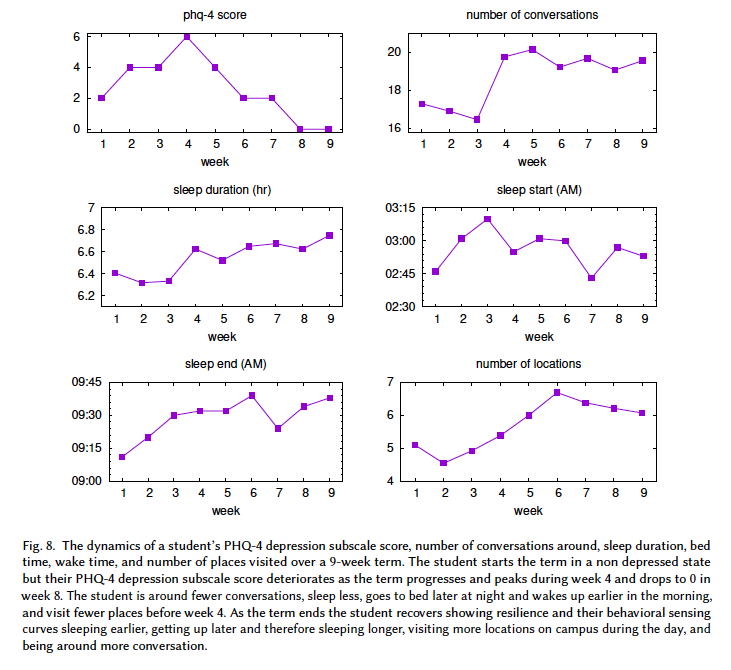
\includegraphics{img/fig9.png}

}

\caption{한 학생의 학기 중 PHQ-4 점수, 대화 횟수, 수면 지속 시간, 취침
시간, 기상 시간, 방문 장소 수 패턴 (13)}

\end{figure}%

이 그래프들은 한 학생의 우울증 수준이 학기 중 특정 시기에 어떻게
변동하는지, 그리고 그에 따라 행동 패턴이 어떻게 변화하는지를 잘
보여줍니다. 이는 학생들의 정신 건강을 모니터링하고, 적절한 시기에 지원을
제공하는 데 중요한 정보를 제공할 수 있습니다. 사례 학생은 PHQ-4 점수가
초기 2주 동안 상승하여 4주차에 최고점을 기록한 후 급격히 감소하여
9주차에는 0이 됩니다. 대화 횟수는 4주에서 대화 횟수가 급격히 증가한 후
안정적으로 유지됩니다. 학기 초기 우울증 악화와 함께 사회적 상호작용이
증가합니다. 학기초 우울증 악화 기간 동안 수면 시간이 감소하다가 이후
안정됩니다. 방문 장소 수는 우울증 악화 기간 동안 적은 수의 장소를
방문하지만 회복되면서 방문 장소 수가 증가하는 패턴을 볼 수 있습니다 .

\section{2) 코로나 기간 동안의 학생 생활 패턴 변화
분석}\label{uxcf54uxb85cuxb098-uxae30uxac04-uxb3d9uxc548uxc758-uxd559uxc0dd-uxc0dduxd65c-uxd328uxd134-uxbcc0uxd654-uxbd84uxc11d}

\begin{figure}[H]

{\centering 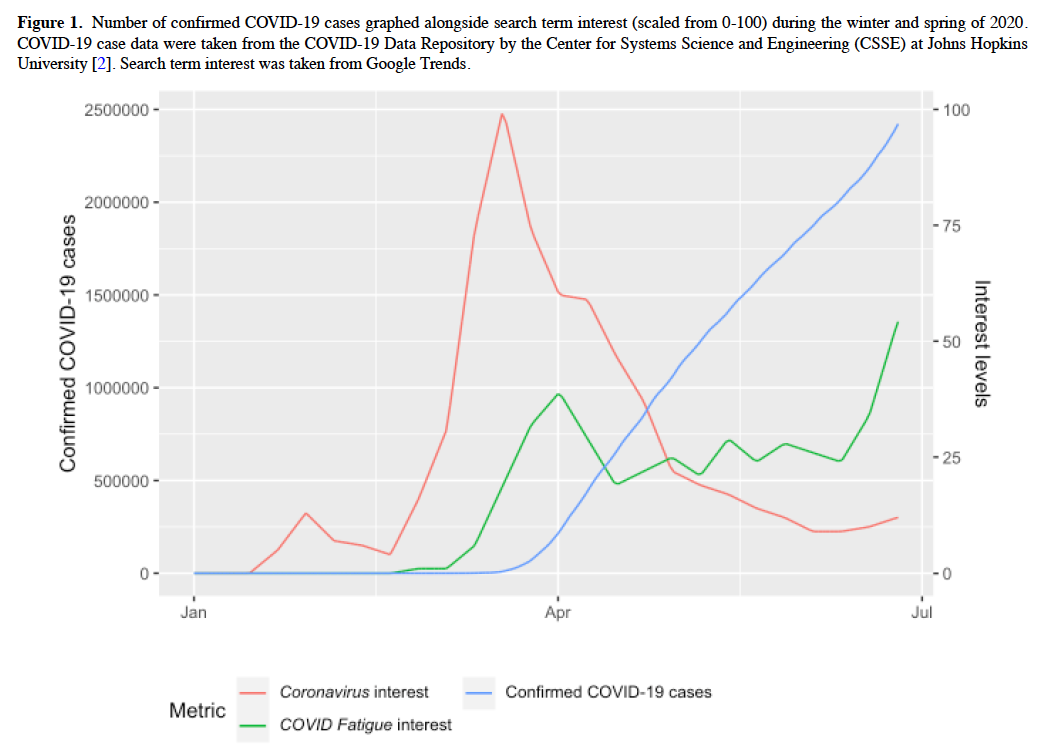
\includegraphics{img/fig10.png}

}

\caption{2020년의 코로나 확진 사례 수와 코로나 바이러스 관심도, 코로나
피로감의 구글 트렌드 관심도 변화 (14)}

\end{figure}%

위 그래프는 존스 홉킨스대에서 수집한 2020년 겨울과 봄 동안 확진된
코로나19 사례 수와 관련된 구글 검색어 관심도를 시각화한 것으로, 팬데믹
초기와 중기 동안 사람들의 정보 검색 행동과 실제 확진자 수의 변화를 잘
보여줍니다. 초기에는 바이러스에 대한 정보 검색이 활발했지만, 시간이
지나면서 코로나 증상에 대한 피로감이 증가했습니다.X축은 시간 (2020년
1월부터 7월까지), Y축의 왼쪽은 확진된 COVID-19 사례 수, Y축의 오른쪽은
관심도 수준을 (0에서 100까지, Google 트렌드 데이터) 나타내고, 파란색
선은 확진된 COVID-19 사례 수, 빨간색 선은 `Coronavirus' 검색어 관심도,
녹색 선은 `COVID Fatigue' 검색어 관심도를 나타냅니다. 확진된 COVID-19
사례 수는(파란색 선) 4월에 급격히 증가하기 시작하여 7월 초에 최고점을
기록합니다. `Coronavirus' 검색어 관심도는(빨간색 선) 3월 중순에 최고점에
도달하고, 5월\textasciitilde6월 이후 관심도가 급격히 감소하여 낮은
수준으로 유지됩니다. `COVID Fatigue' 검색어 관심도는 (녹색 선)
3월\textasciitilde4월에 관심도가 증가하여 4월 초에 첫 번째 피크에
도달합니다. 이후 관심도가 약간 감소했다가 6월 중순부터 다시 증가합니다.

4월 이후, 확진 사례 수가 계속 증가하는 반면, 'Coronavirus'에 대한
관심도는 감소하는 것은 사람들이 바이러스 자체에 대한 정보보다는 다른
주제에 더 관심을 가지기 시작했음을 시사합니다. 6월 이후 'COVID
Fatigue'에 대한 관심도가 다시 증가하는 것은 팬데믹이 장기화되면서
피로감이 더욱 심화되었음을 보여줍니다.

해당 데이터는 공중 보건 메시지 전달과 같은 커뮤니케이션 전략을 수립하는
데 중요한 인사이트를 제공하며, 팬데믹 동안 사람들의 정보 필요와 감정적
반응을 이해함으로써 더 나은 대응 전략을 마련할 수 있습니다.

\begin{figure}[H]

{\centering 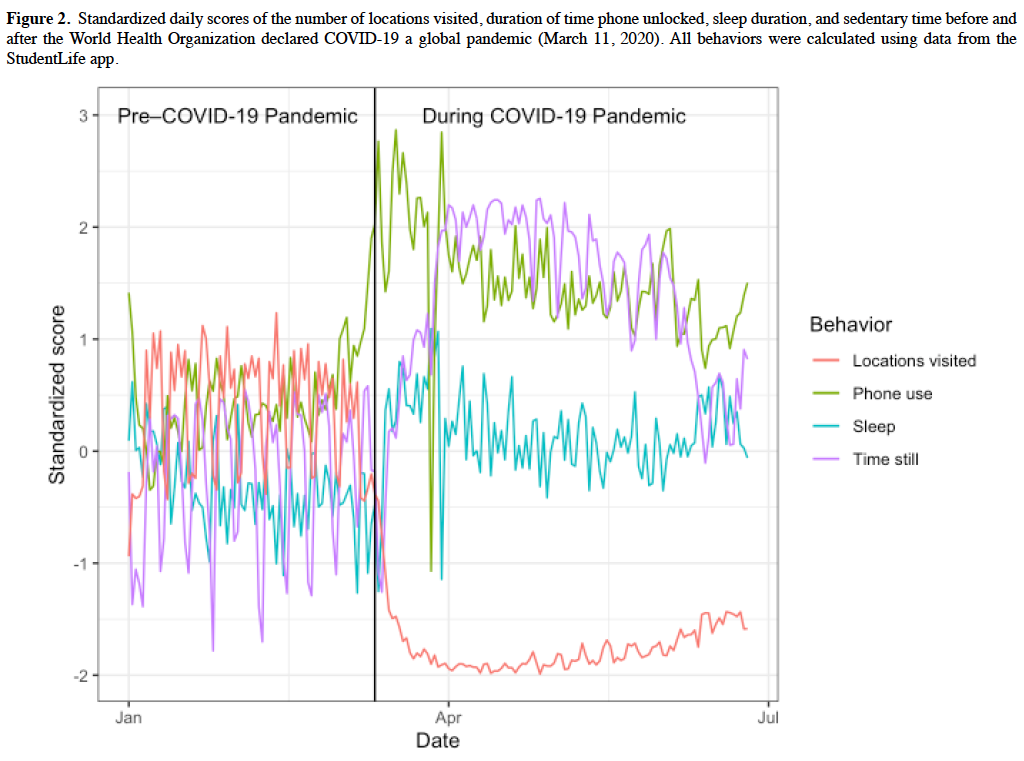
\includegraphics{img/fig11.png}

}

\caption{2020년 코로나 팬데믹 기간의 StudentLife 앱에 기록된 학생 활동
변화 (14)}

\end{figure}%

위 그래프는 COVID-19 팬데믹 이전과 이후의 학생들의 일상 행동 변화를
시각화한 것입니다. 여기에는 방문한 장소 수, 핸드폰 사용 시간, 수면 시간,
움직임이 없던 시간이 표준화 지표로 표현되어 있습니다. 팬데믹 선언 후
방문한 장소 수가 급격히 감소하고, 핸드폰 사용 시간과 정지 상태의 시간이
급격히 증가합니다. 또한 수면 시간도 팬데믹 이전보다 증가하는 경향을
보입니다. WHO가 COVID-19 팬데믹을 선언한 날짜 (2020년 3월 11일)전에는
모든 행동 지표가 변동성이 큽니다. 팬데믹 선언 직후 모든 행동 지표에
급격한 변화가 관찰됩니다. 팬데믹 동안(Dur방문한 장소 수는 낮은 수준을
유지하지만, 점차 증가하는 경향이 있습니다. 핸드폰 사용 시간은 팬데믹
선언 직후 급격히 증가합니다. 이는 학생들이 집에 머무르면서 온라인 활동과
소셜 미디어 사용이 증가했음을 시사합니다. 수면 시간과~정지 상태 시간은
변동이 있지만 팬데믹 이전보다 높은 수준을 유지합니다.

\begin{figure}[H]

{\centering 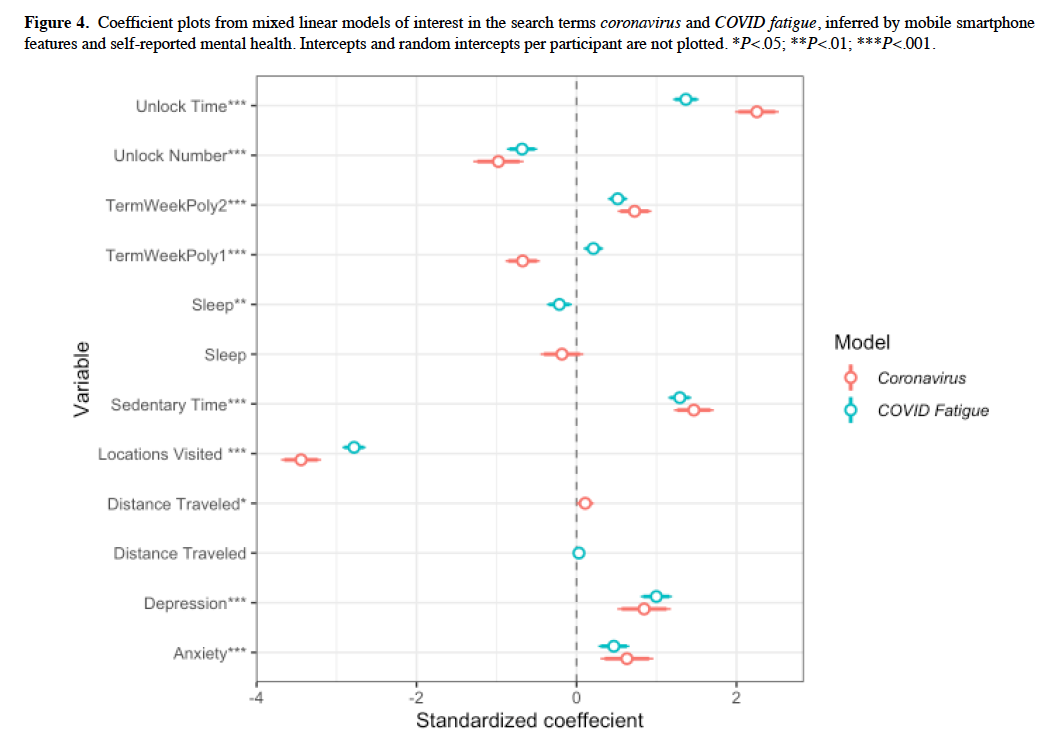
\includegraphics{img/fig12.png}

}

\caption{코로나 바이러스, 코로나 피로의 관심도가 학생 활동의 영향에 대한
회귀 분석 시각화 (14)}

\end{figure}%

위 그래프(Coefficient plot)은 코로나 바이러스, 코로나 피로의 관심도와
학생 활동의 영향에 대한 회귀 분석 결과를 시각화한 그래프입니다. X축의
계수 값(Coefficient Value)이 클수록 해당 변수의 영향력이 크고, 계수 값이
양수면 해당 변수가 종속 변수에 정(+)의 영향을, 음수면 부(-)의 영향을
미칩니다. 이 플롯을 통해 어떤 변수가 중요한지, 그리고 그 영향력이 어떻게
되는지를 직관적으로 파악할 수 있습니다.

위 그래프에서 코로나 바이러스, 코로나 피로의 관심도는 스마트폰 사용
시간, 정적 활동의 증가와 관련이 있으며, 이동 거리와 방문 장소 수의
감소와 관련이 있습니다. 또한 우울과 걱정도 코로나 관심도가 양의 영향을
미칩니다.

\section{3) 코로나 기간 전후의 학생 생활 및 정신 건강 상태에 대한 데이터
분석}\label{uxcf54uxb85cuxb098-uxae30uxac04-uxc804uxd6c4uxc758-uxd559uxc0dd-uxc0dduxd65c-uxbc0f-uxc815uxc2e0-uxac74uxac15-uxc0c1uxd0dcuxc5d0-uxb300uxd55c-uxb370uxc774uxd130-uxbd84uxc11d}

이 연구는 대학생들의 정신 건강 변화를 코로나 기간을 포함하여 추적한
연구로서, 연구진은 모바일 센싱 소프트웨어를 사용하여 4년 동안 200명
이상의 대학생들의 실시간 활동 데이터를 수집했습니다.

\begin{figure}[H]

{\centering 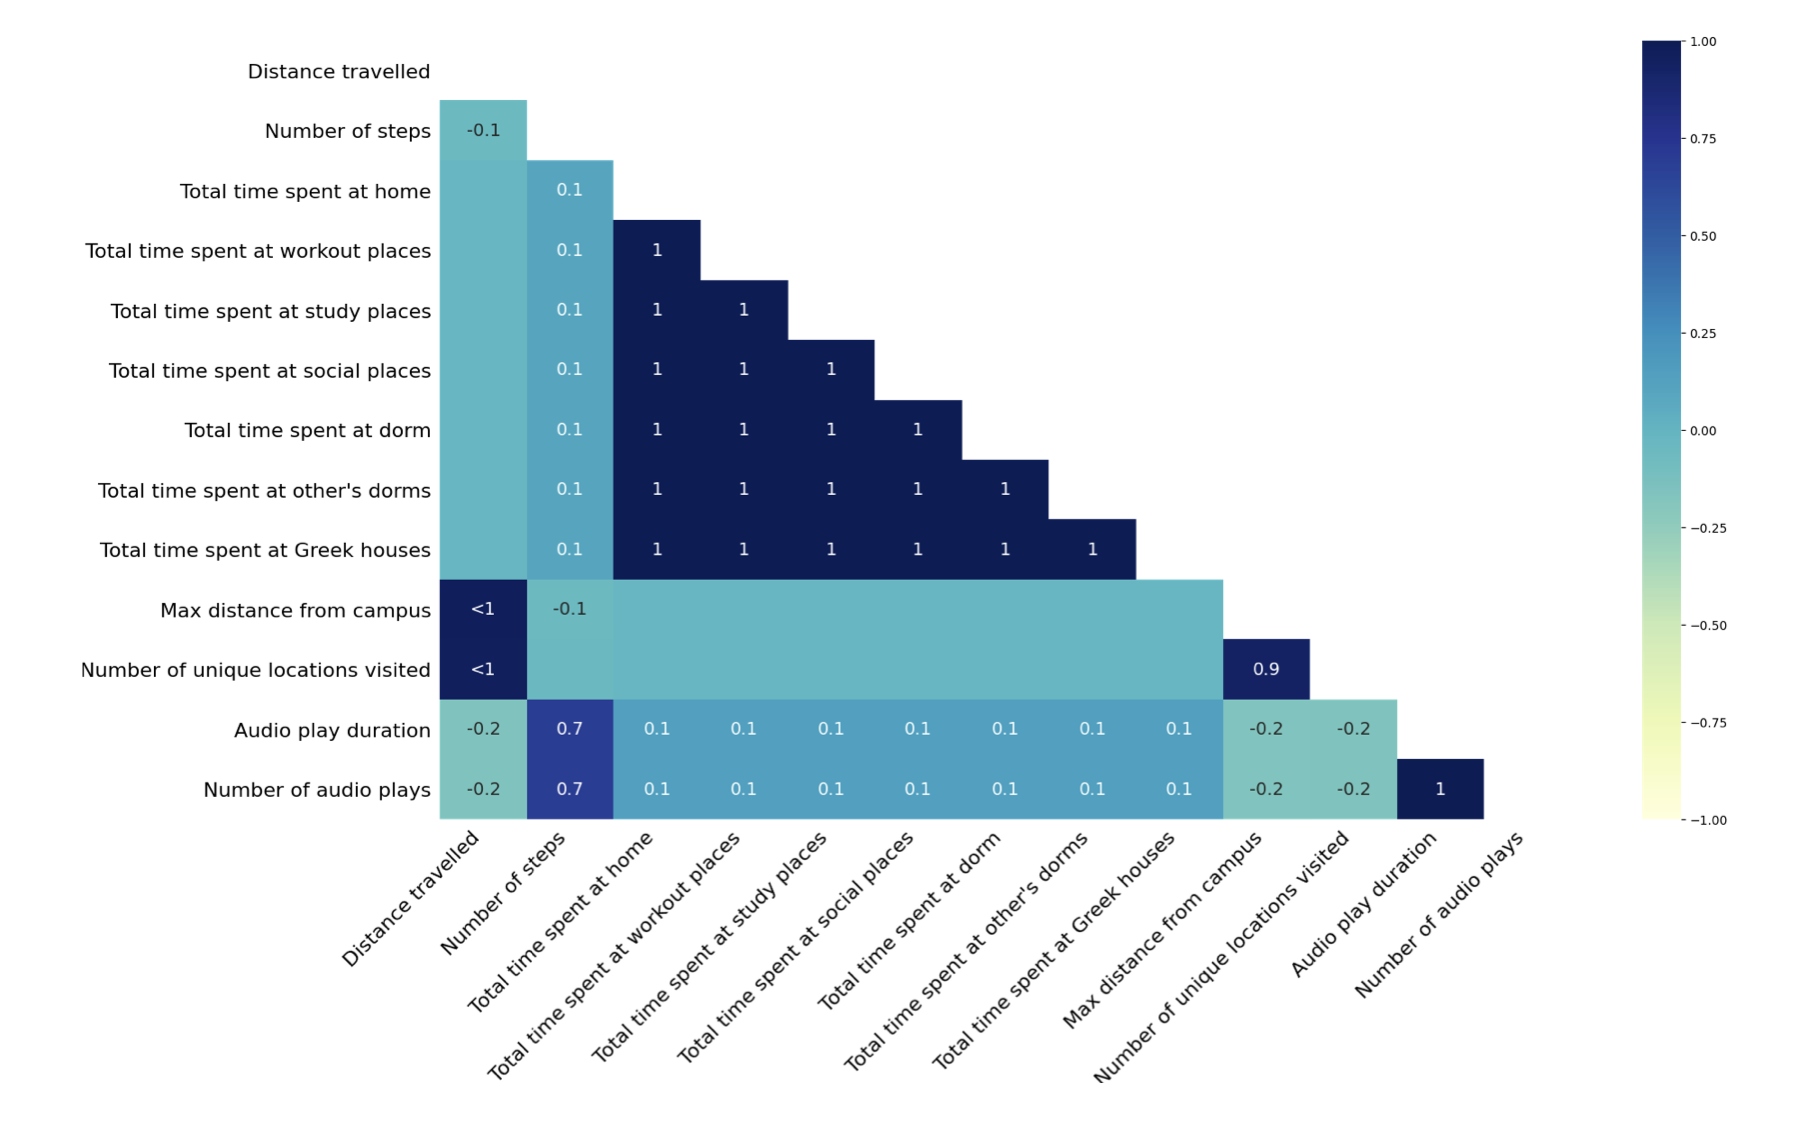
\includegraphics{img/fig13.png}

}

\caption{실험의 센싱 데이터 결측값(Missing Values) 간의 상관관계 그래프
(15)}

\end{figure}%

Nullity Correlation은 데이터 분석에서 결측값(Missing Values) 간의
상관관계를 나타내는 용어입니다. 특정 변수의 결측값 존재 여부와 다른
변수의 결측값 존재 여부 사이의 관계를 측정합니다. 예를 들어, 두 변수
모두 결측값이 있는 경우, 이 변수들은 높은 Nullity Correlation 값을 가질
것입니다. 이는 한 변수의 데이터가 결측되면 다른 변수도 결측될 가능성이
높다는 것을 의미합니다.

{[}그림 14{]}에서, 대부분의 위치 관련 특성들은 1의 값을 가지는데, 이는
하나의 위치 특성이 나타나면 다른 위치 특성도 거의 항상 나타난다는 것을
의미합니다. 위치 특성은 GPS 데이터의 가용성에 따라 달라지기 때문에, GPS
데이터가 있을 때는 위치 특성들이 모두 존재하거나, 없을 때는 모두
존재하지 않는 것이 논리적입니다. 1.0 상관관계에 대한 예시로 ****``Total
time spent at social places''와 ``Total time spent at other's dorms''
(사회적 장소에서 보낸 시간과 다른 기숙사에서 보낸 시간)을 보면 두 장소의
데이터는 동시에 측정되었습니다. 그리고 ``Number of audio plays''와
``Audio play duration'' (오디오 재생 횟수와 오디오 재생 시간)의 0.7
상관관계는 두 기능이 자주 함께 나타남을 의미합니다. 오디오를 재생할수록
재생 시간도 증가하기 때문에 논리적인 결과입니다. 반면에 ``Audio play
duration''과 ``Total time spent at study places'' (오디오 재생 시간과
공부 장소에서 보낸 시간)간의 음의 상관관계는 상관관계가 없다고 볼 수
있습니다. 예를 들어, 운동이나 공부를 할 때 오디오를 재생하는 시간이
감소할 수 있습니다.

\begin{figure}[H]

{\centering 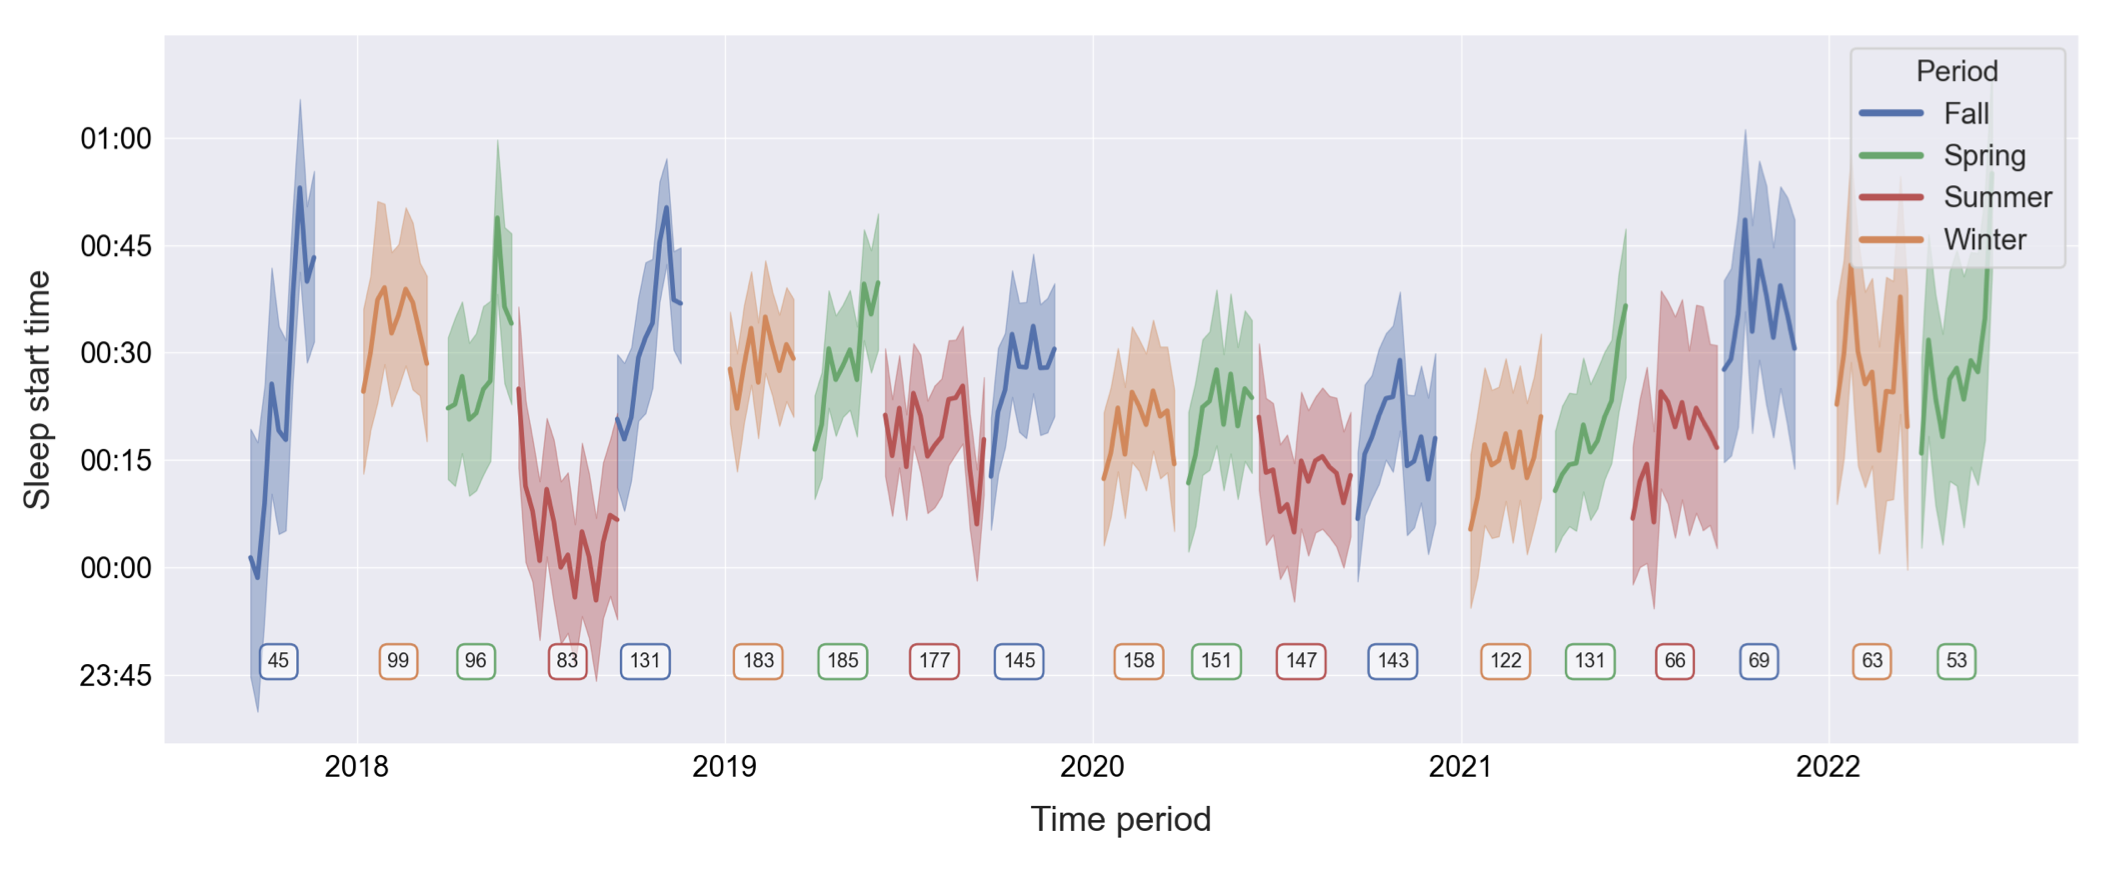
\includegraphics{img/fig14.png}

}

\caption{데이터 수집 기간 동안의 학생들의 수면 시작 시간 패턴 변화 (15)}

\end{figure}%

해당 그래프는 2018년부터 2022년까지 학기와 연도에 따른 학생들의 수면
시작 시간의 변화를 보여줍니다. 여름 학기 동안 학생들이 더 일찍 잠드는
경향이 있으며, 학기 말로 갈수록 수면 시간이 늦어지는 패턴이 관찰됩니다.
그리고 가을 학기(파랑)와 겨울 학기(주황)는 비교적 수면 시작 시간이
일정하게 유지되지만, 봄 학기(초록)와 여름 학기(빨강)는 더 큰 변동성을
보입니다. 각 학기의 참여자 수는 그래프 하단의 사각형에 표시되어
있습니다. 예를 들어, 2018년 가을 학기에는 45명이 데이터를 제공한 반면,
2021년 봄 학기에는 122명이 데이터를 제공하였습니다. 학기마다 다른
참여자수는 데이터의 신뢰성에 영향을 미칠 수 있습니다.이러한 정보를
통하여 학생들의 수면 습관을 이해하고, 건강한 수면 습관을 촉진하기 위한
캠퍼스 정책을 개발할 수 있습니다.

\begin{figure}[H]

{\centering 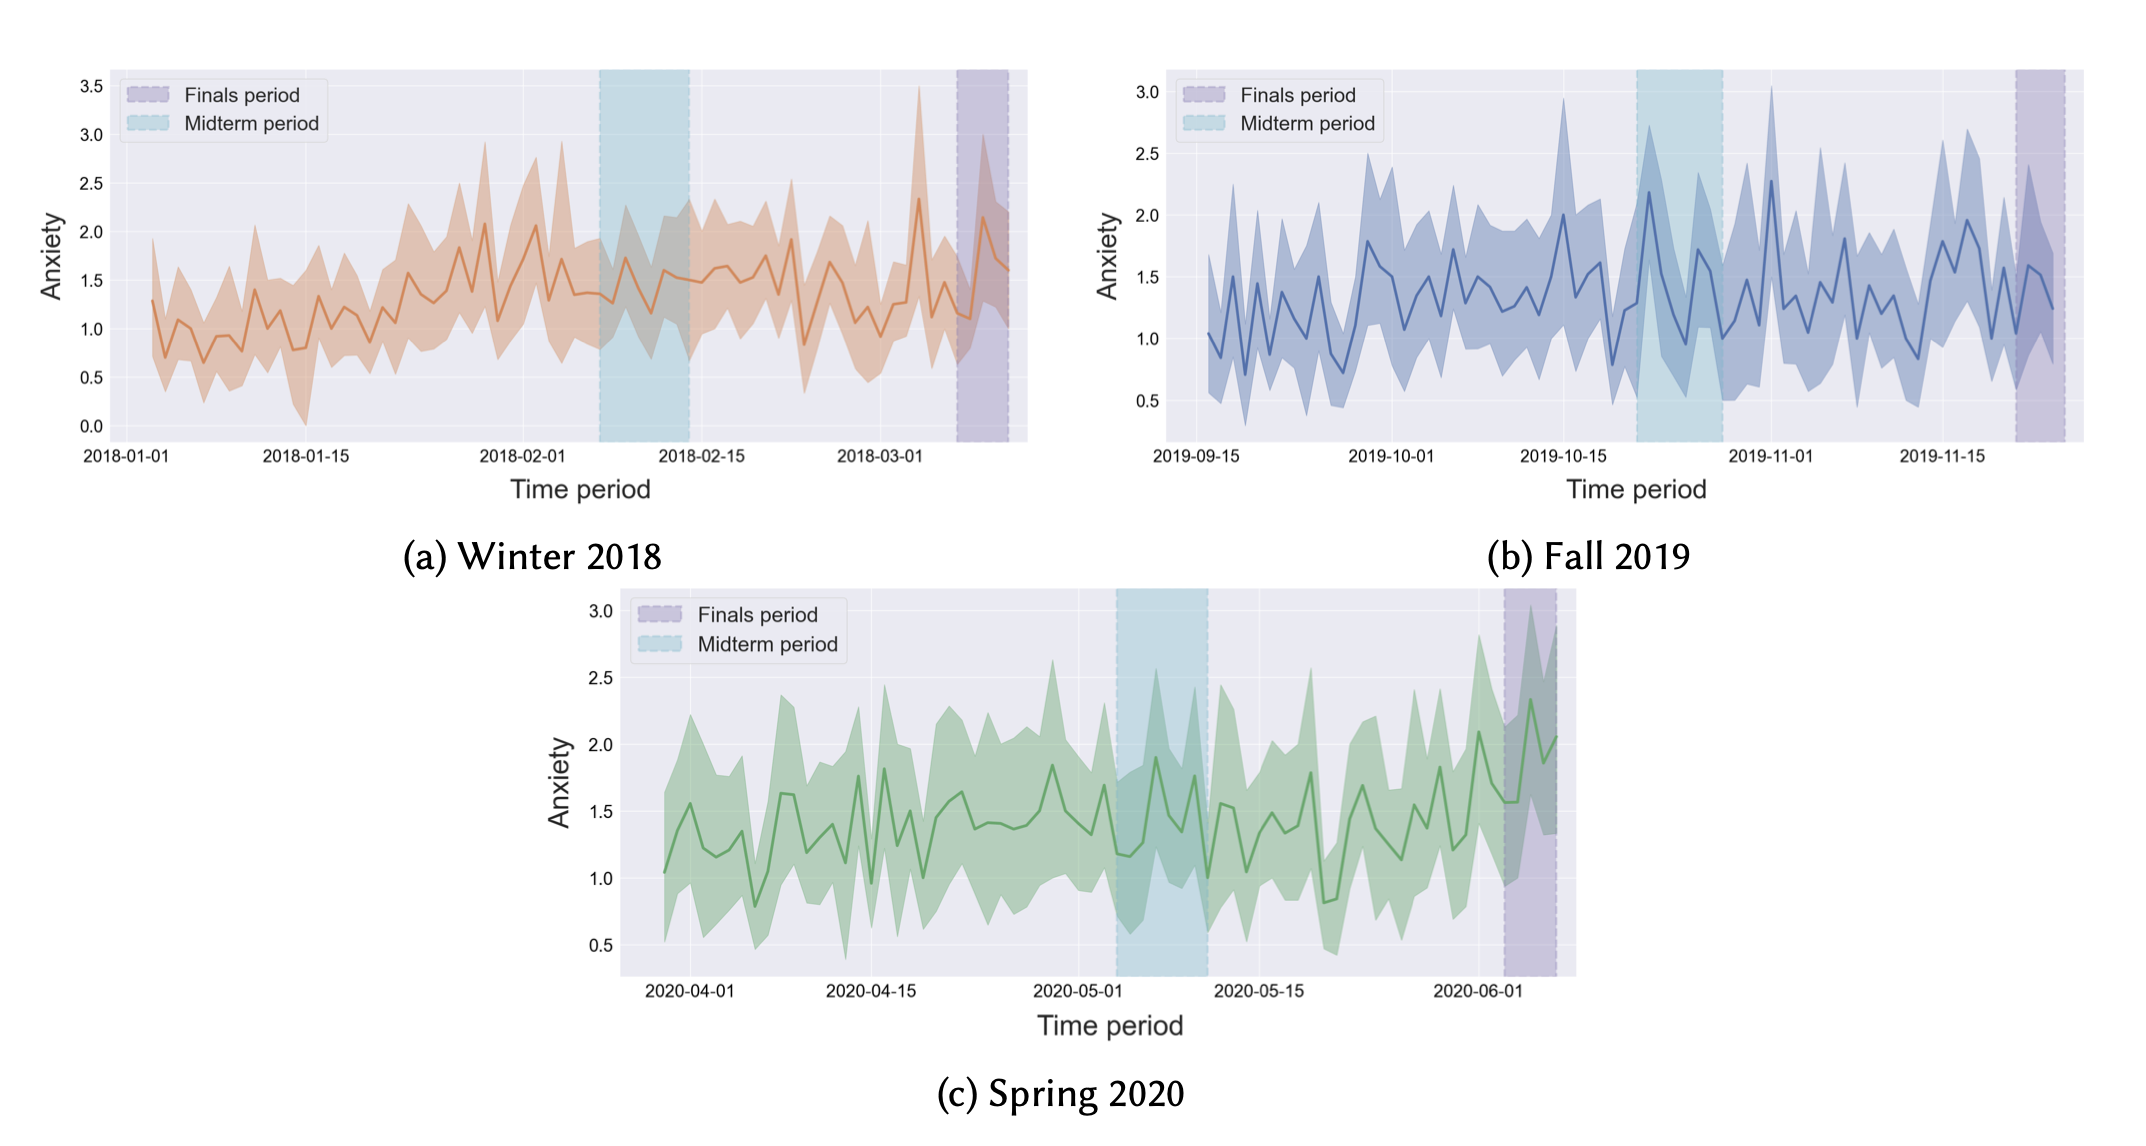
\includegraphics{img/fig15.png}

}

\caption{학기별 학생들의 불안 지수 변화 (15)}

\end{figure}%

이 그래프는 학생들이 중요한 학업 기간 동안 불안을 더 많이 느낀다는 것을
시각적으로 보여줍니다. 특히 중간고사와 기말고사 기간 동안 불안 점수가
상승하는 경향이 명확하게 나타납니다. 2018년 겨울 학기와 2020년 봄 학기는
불안 점수의 변동 폭이 크지만, 2019년 가을 학기는 비교적 안정적인 차이가
있어 학기별로 불안 지수가 다른 특징이 있습니다. 이러한 정보는 학생들의
학업 스트레스를 줄이고, 정신 건강을 지원하기 위한 정책을 개발하는 데
중요한 데이터로 활용될 수 있습니다.

\begin{figure}[H]

{\centering 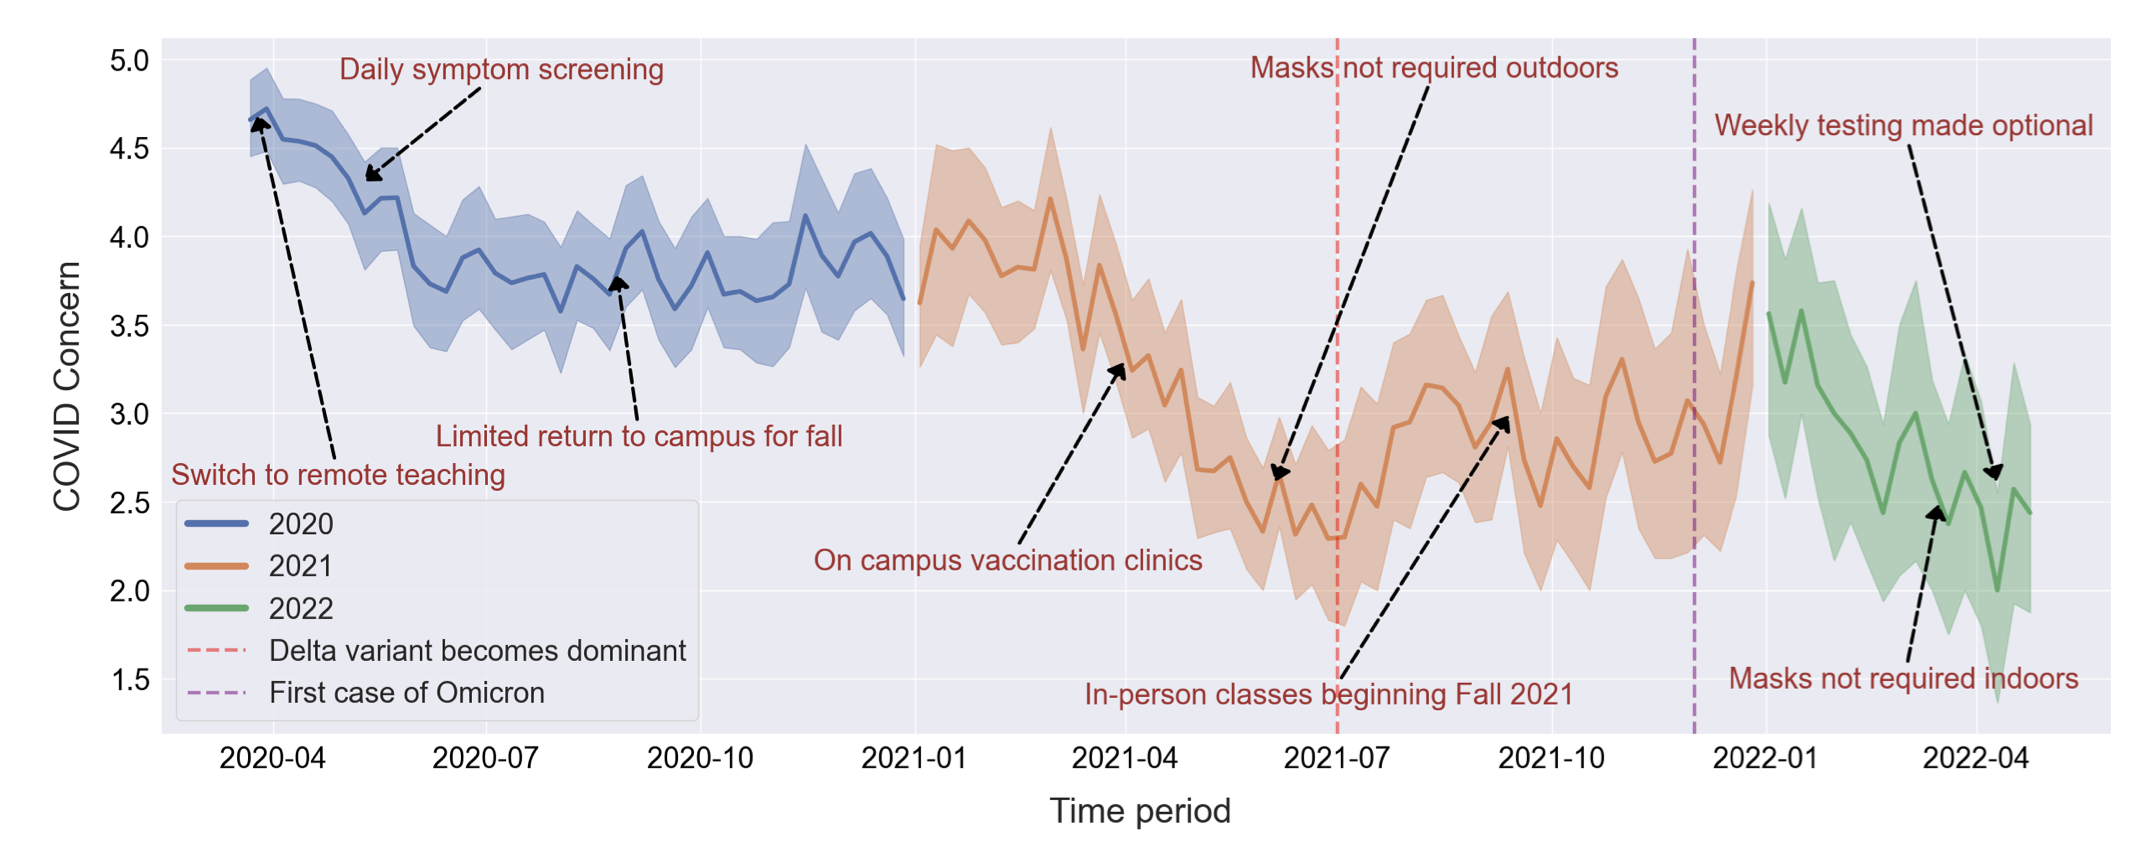
\includegraphics{img/fig16.png}

}

\caption{시간의 흐름에 따른 코로나 걱정 지수 변화 (15)}

\end{figure}%

이 그래프는 코로나 팬데믹 기간 동안 주요 코로나 이벤트에 따른 COVID-19에
대한 학생들의 걱정 정도를 보여줍니다. 중요한 캠퍼스 이벤트 및 조치들이
학생들의 걱정 수준에 큰 영향을 미쳤음을 알 수 있습니다. 이러한 데이터는
팬데믹 대응 및 학생 지원 전략을 수립하는 데 인사이트를 제공할 수
있습니다.

주요 이벤트와 걱정 지수의 변화:

\begin{itemize}
\tightlist
\item
  원격 수업 전환 (2020년 4월): 걱정 수준이 상당히 낮아지는 효과가
  있습니다.
\item
  일일 증상 검사 도입 (2020년 5월): 초기 팬데믹 대응 조치로, 걱정 수준이
  높지만 점차 감소합니다.
\item
  캠퍼스 복귀 제한적 허용 (2020년 10월): 걱정 수준이 다시 약간
  상승합니다.
\item
  백신 클리닉 도입 (2021년 4월): 걱정 수준이 크게 감소하는 주요
  요인입니다.
\item
  마스크 착용 완화 (2021년 6월, 2022년 4월): 걱정 수준이 감소하는 경향을
  보입니다.
\item
  델타 변이 및 오미크론 변이 출현 (2021년 7월, 2022년 1월): 새로운
  변이의 출현으로 걱정 수준이 다시 증가합니다.
\end{itemize}

이상의 데이터 분석 사례와 같이 여러분의 실습 주제와 관련한 데이터 분석
보고서나 논문을 찾아보고, 제시된 데이터의 분석 표나 그래프를 해석하여
디자인 주제에 대한 인사이트를 발견해보세요.

(문헌 10) Dartmouth College, ``StudentLife Study'', (2024.7.24),
\href{https://studentlife.cs.dartmouth.edu/}{https://studentlife.cs.dartmouth.edu}

(문헌 11) Kaggle, ``College Experience Study Dataset'', (2024.7.31)
\url{https://www.kaggle.com/datasets/subigyanepal/college-experience-dataset?resource=download}

(문헌 12) Rui Wang, et al., ''SmartGPA: How Smartphones Can Assess and
PredictAcademic Performance of College Students'', UbiComp '15,
September 07-11, 2015, Osaka, Japan

(문헌 13) R. Wang et. al., ``Tracking Depression Dynamics in College
Students Using MobilePhone and Wearable Sensing'', Proceedings of the
ACM on Interactive, Mobile, Wearable and Ubiquitous Technologies, Vol.
2, No.~1, Article 43. (2018).

(문헌 14) D. L Mack, et al., ``Mental Health and Behavior of College
Students During theCOVID-19 Pandemic: Longitudinal Mobile Smartphone
andEcological Momentary Assessment Study, Part II'', JOURNAL OF MEDICAL
INTERNET RESEARCH, vol.~23, iss. 6, e28892 (2021)

(문헌 15) Subigya Nepal, et al.~``Capturing the College Experience: A
Four-Year Mobile Sensing Study of Mental Health, Resilience and Behavior
of College Students during the Pandemic.'' Proceedings of the ACM on
Interactive, Mobile, Wearable and Ubiquitous Technologies. (2024)

\chapter{ch4. EDA를 위한 데이터 분석
도구들}\label{ch4.-edauxb97c-uxc704uxd55c-uxb370uxc774uxd130-uxbd84uxc11d-uxb3c4uxad6cuxb4e4}

\section{Google Analytics (GA)}\label{google-analytics-ga}

Google Analytics는 웹사이트와 앱의 사용자 행동을 추적하고 분석하여,
마케팅 전략을 개선하고 사용자 경험을 최적화하는 데 도움을 주는
도구입니다. 이를 통해 사용자들이 어떤 경로로 사이트에 도착했는지, 어떤
페이지에서 얼마나 머무르는지, 어떤 행동을 하는지 등을 상세히 분석할 수
있습니다. 서비스에 가입하면 데이터 분석이 필요한 웹 서비스에 GA와
연계하는 코드를 삽입하여 데이터를 추출하고, 다양한 GUI 메뉴로 데이터
현황을 탐색할 수 있습니다. (16)

\href{https://marketingplatform.google.com/intl/ko/about/analytics/features/}{애널리틱스
기능}

\section{주요 서비스}\label{uxc8fcuxc694-uxc11cuxbe44uxc2a4}

\begin{itemize}
\item
  데이터 수집 및 관리

  웹사이트와 앱의 데이터를 통합하여 분석할 수 있고, 다양한 플랫폼과
  기기에서 발생하는 데이터를 정확하게 추적합니다.
\item
  분석 및 통계

  \begin{itemize}
  \tightlist
  \item
    사용자 세그먼트: 특정 기준에 따라 사용자 그룹을 세분화하고 각 그룹의
    행동을 분석할 수 있습니다.
  \item
    행동 분석: 사용자의 페이지 방문, 클릭, 이벤트 등 다양한 행동
    데이터를 분석합니다.
  \item
    실시간 데이터: 실시간으로 웹사이트 방문자 수, 현재 활동 중인 페이지
    등을 모니터링할 수 있습니다.
  \end{itemize}
\item
  보고 및 시각화

  맞춤형 대시보드로 중요한 데이터를 한눈에 볼 수 있습니다. 데이터를
  그래프와 차트로 시각화하여 쉽게 이해하고 분석할 수 있고, PDF, Excel 등
  다양한 형식으로 보고서를 내보낼 수 있습니다.
\item
  통합 및 확장

  \begin{itemize}
  \tightlist
  \item
    Google Ads, Google Tag Manager, Firebase 등 다른 Google 도구와
    원활하게 연동됩니다.
  \item
    API 지원: 다양한 API를 통해 데이터를 추출하고 맞춤형 솔루션을 구축할
    수 있습니다.
  \end{itemize}
\item
  머신러닝 및 인사이트

  머신러닝을 활용하여 자동으로 목표를 설정하고 중요한 인사이트를
  제공합니다. 사용자의 미래 행동을 예측하고 이에 맞춘 전략을 수립할 수
  있습니다.
\item
  단점: 고급 기능을 활용하려면 일정 수준 이상의 기술 지식이 필요할 수
  있습니다. 그리고 대규모 트래픽이 발생하는 웹사이트에서는 샘플링
  데이터를 제공하여 전체 데이터를 반영하지 않을 수 있습니다.

  \begin{figure}[H]

  {\centering 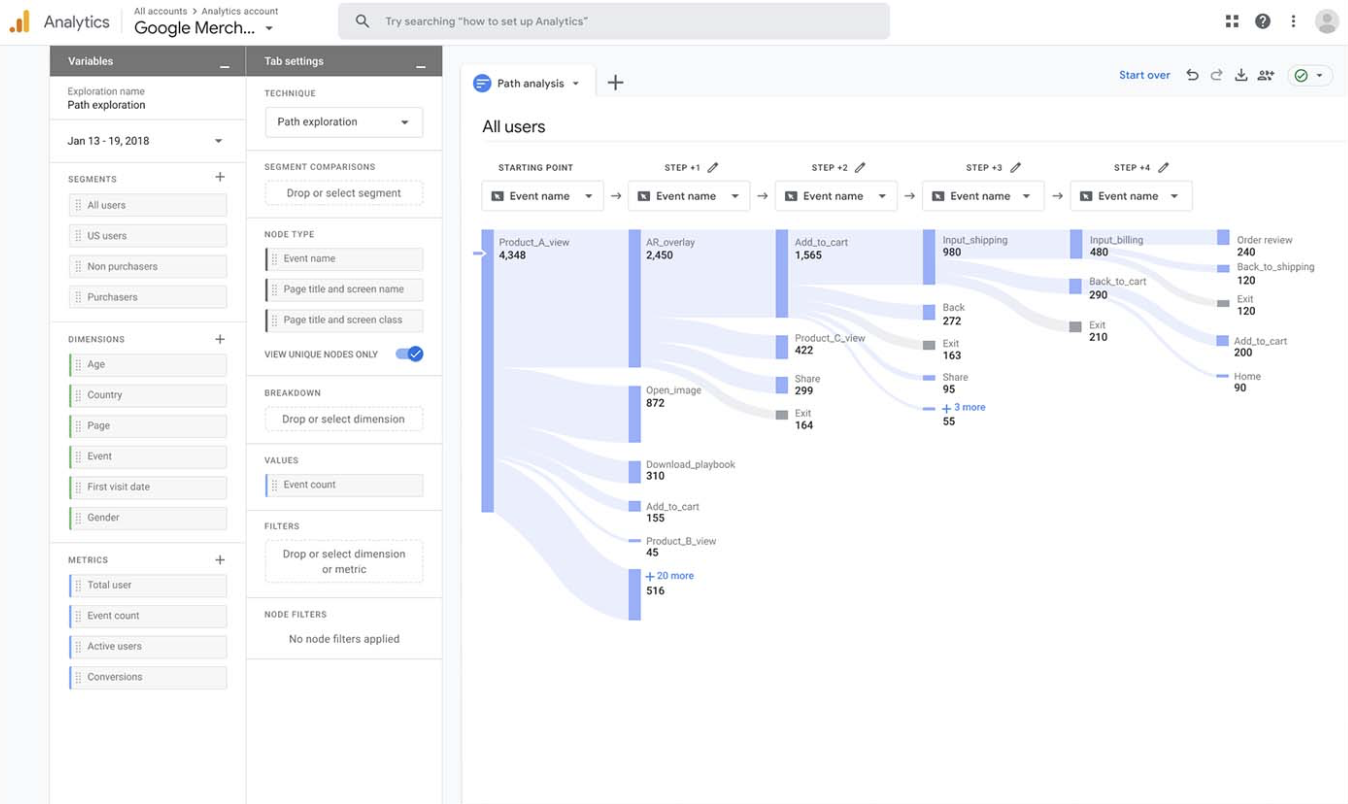
\includegraphics{img/fig17.png}

  }

  \caption{Google Analytics의 데이터 시각화 화면}

  \end{figure}%
\end{itemize}

\section{Power BI}\label{power-bi}

Power BI는 Microsoft에서 제공하는 비즈니스 분석 서비스로, 데이터를
시각화하고 공유 가능한 보고서를 생성하며, 인사이트를 도출하는 클라우드
기반 솔루션입니다. 사용 방법은 Power BI Desktop 설치 후, 다양한 데이터
소스를(Excel, SQL Server 등) 연결하고, 실시간 데이터 가져오기 하여
분석을 시행합니다. Power BI Desktop에서 보고서 작성 후에는 Power BI
서비스(웹)에서 공유 및 대시보드를 관리합니다. 이를 통해 사용자들은
데이터 기반의 의사 결정을 내릴 수 있습니다. (17)

\href{https://powerbi.microsoft.com/ko-kr/guidedtour/power-platform/power-bi/2/1}{Power
BI 둘러보기}

\section{주요 서비스}\label{uxc8fcuxc694-uxc11cuxbe44uxc2a4-1}

\begin{itemize}
\tightlist
\item
  데이터 통합: 다양한 데이터 소스(엑셀, SQL 데이터베이스, 클라우드
  서비스 등)와 연결하여 데이터를 통합합니다. 특히 Microsoft 제품과의
  통합에 강점을 가집니다.
\item
  대시보드 생성: 실시간 데이터 시각화와 대시보드를 생성하여 데이터를
  한눈에 파악할 수 있습니다.
\item
  보고서 작성: 다양한 시각화 도구를 사용하여 상세한 보고서를 작성하고
  분석할 수 있습니다.
\item
  모바일 접근성: 모바일 앱을 통해 언제 어디서나 데이터를 조회하고 분석할
  수 있습니다.
\item
  AI 통합: 인공지능 기능을 통해 예측 분석과 자동화된 인사이트를
  제공합니다
\item
  사용자 친화적 인터페이스와 협업 지원: 직관적이고 사용하기 쉬운
  인터페이스를 제공하고, 팀 내에서 보고서를 공유하고 협업할 수 있습니다.
\item
  단점: 초보자에게는 초기 설정이 복잡할 수 있습니다. 무료 버전의 기능이
  제한적이며, 대용량 데이터를 처리하는 데 제한이 있을 수 있습니다.
\end{itemize}

\begin{figure}[H]

{\centering 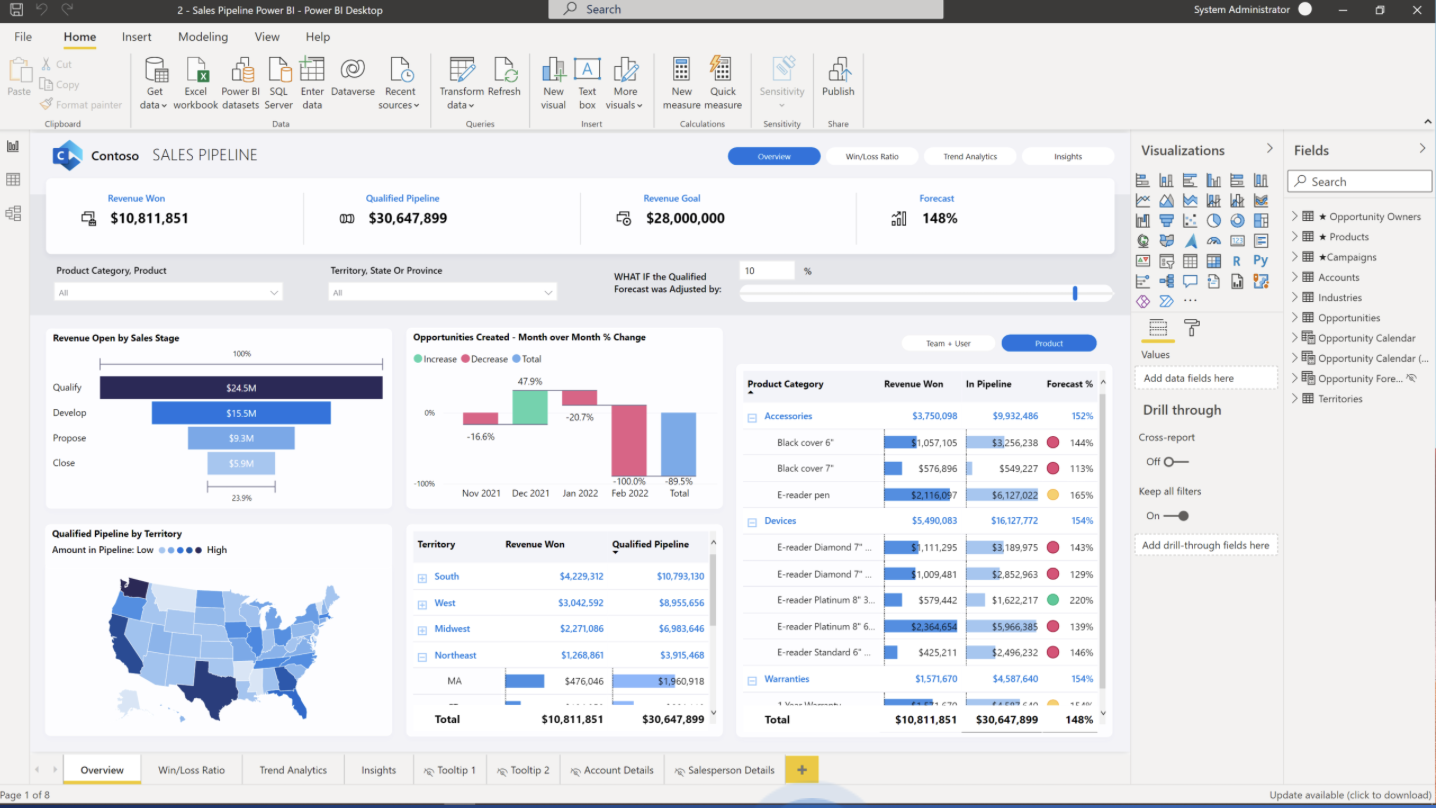
\includegraphics{img/fig18.png}

}

\caption{Power BI의 데시보드 구성 화면}

\end{figure}%

\section{Tableau}\label{tableau}

Tableau는 데이터를 시각적으로 분석하고 이해할 수 있게 돕는 비즈니스
인텔리전스(BI) 도구입니다.

Tableau는 고급 데이터 시각화 기능에 강점을 갖고 있어, 히트맵, 트리맵,
버블 차트 등 다양한 고급 시각화 기능을 제공하고, 사용자가 대시보드를
인터렉티브하게 데이터 탐색을 할 수 있으며, 데이터 시각화를 스토리 형태로
구성해 프레젠테이션하고, 지리적 데이터를 시각화하고 분석하는 강력한
기능을 제공합니다. (18)

\href{https://www.tableau.com/ko-kr/products/tableau}{Tableau product}

\section{주요 서비스}\label{uxc8fcuxc694-uxc11cuxbe44uxc2a4-2}

\begin{itemize}
\item
  데이터 통합: 다양한 소스의 데이터를 통합하여 일관된 분석 가능합니다.
\item
  시각화 도구: 드래그 앤 드롭 방식으로 손쉽게 고급 시각화 차트와
  대시보드를 생성합니다.
\item
  AI 및 ML 통합: 인공지능과 머신러닝을 통해 예측 분석 및 인사이트를
  제공합니다.
\item
  단점: 고급 기능을 완전히 익히는 데 시간이 필요합니다.

  \begin{figure}[H]

  {\centering 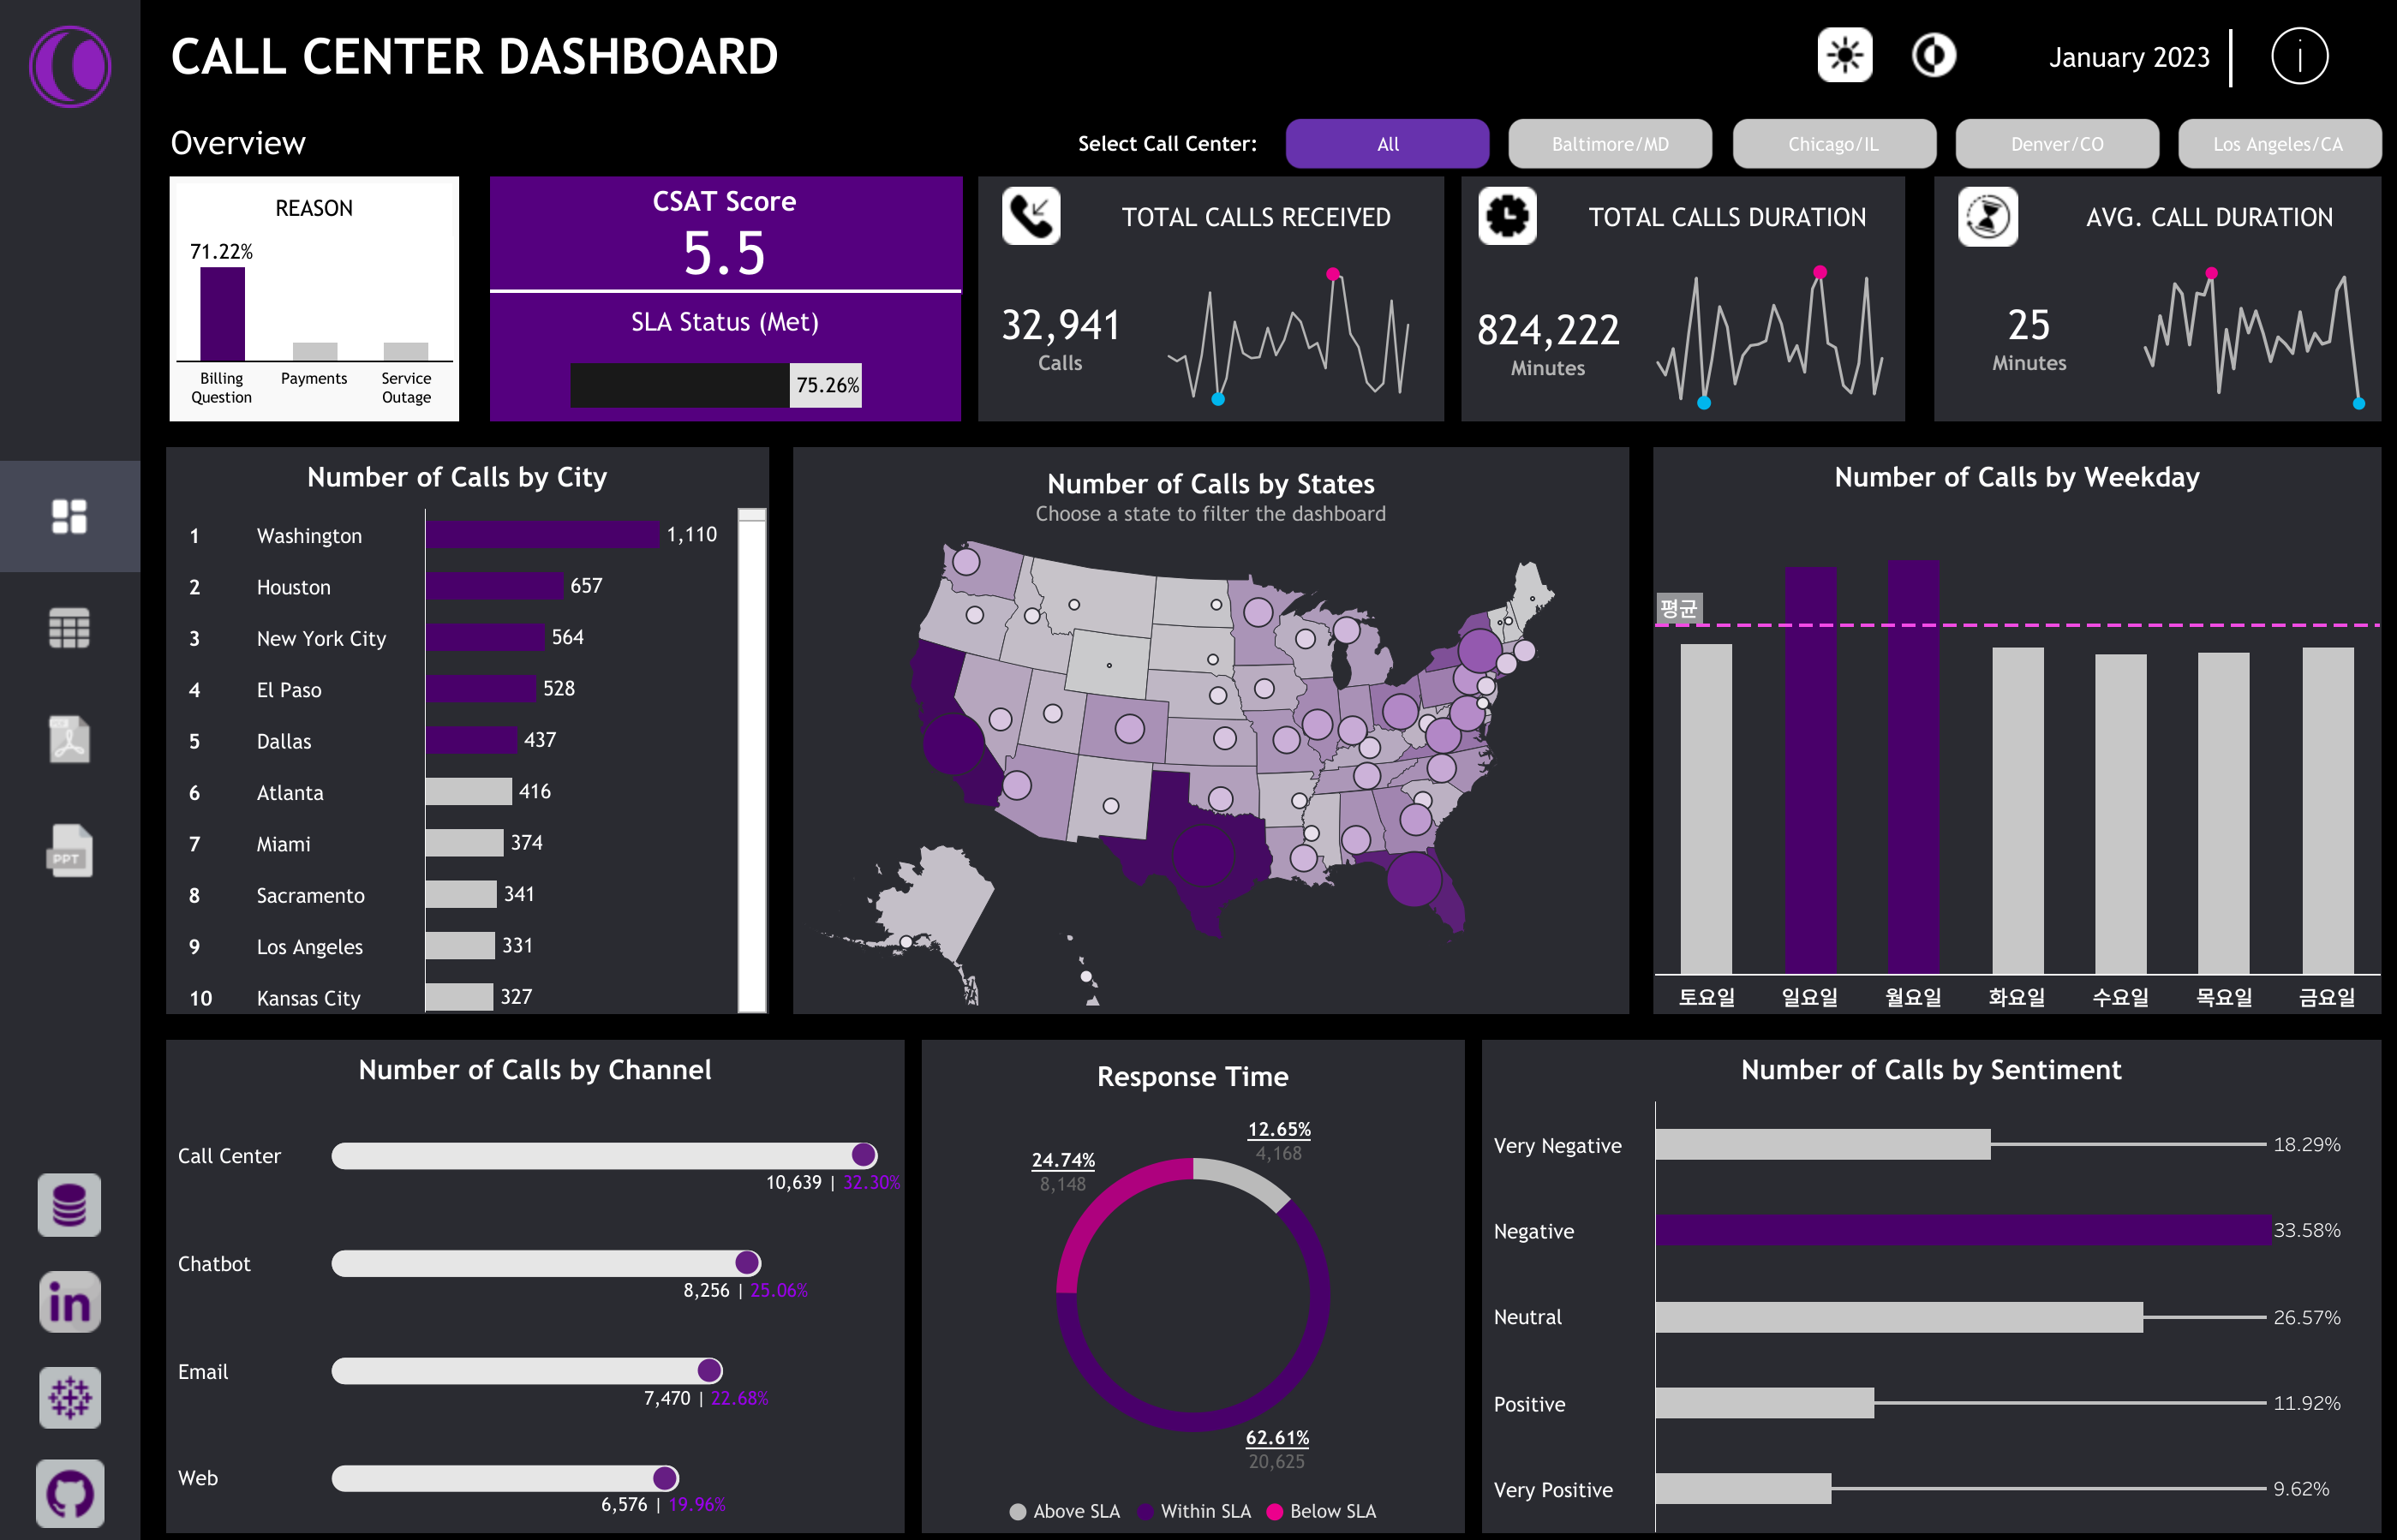
\includegraphics{img/fig19.png}

  }

  \caption{Tableau를 사용한 인터렉티브 대시보드}

  \end{figure}%
\end{itemize}

이 세가지 서비스는 세계적으로 가장 많이 사용되는 데이터 분석 서비스이고,
최근에는 AI 기술을 사용한 시각화 및 예측 서비스가 강화되는 추세입니다.
Google Analytics는 주로 웹사이트 분석에, Power BI는 비즈니스 인텔리전스
및 데이터 분석에, Tableau는 고급 데이터 시각화에 좀 더 특화되어 있다고
할 수 있습니다.

\section{Beusable}\label{beusable}

Beusable은 UX를 위한 데이터 분석에 특화된 국내 서비스로, 사용자 경험을
개선하기 위해 시각화된 데이터 분석 기능을 제공합니다. 주요 기능으로는
Journey Map과 UX Heatmap이 있으며, 이를 통해 고객 여정을 시각적으로
파악하고, 문제 구간을 분석하여 개선안을 도출할 수 있습니다. 설치가
간편하고, 직관적인 UI를 제공합니다. (19)

\href{https://www.beusable.net/ko/}{Why Beausable}

\section{주요 서비스}\label{uxc8fcuxc694-uxc11cuxbe44uxc2a4-3}

\begin{itemize}
\tightlist
\item
  Journey Map: 고객의 전환 과정을 시각화하여 분석합니다.
\item
  UX Heatmap: 페이지 내 사용자 행동을 시각화하여 문제점을 파악합니다.
\item
  간편한 설치: 한 줄의 코드 설치로 데이터 수집 및 분석이 가능합니다.
\end{itemize}

\begin{figure}[H]

{\centering 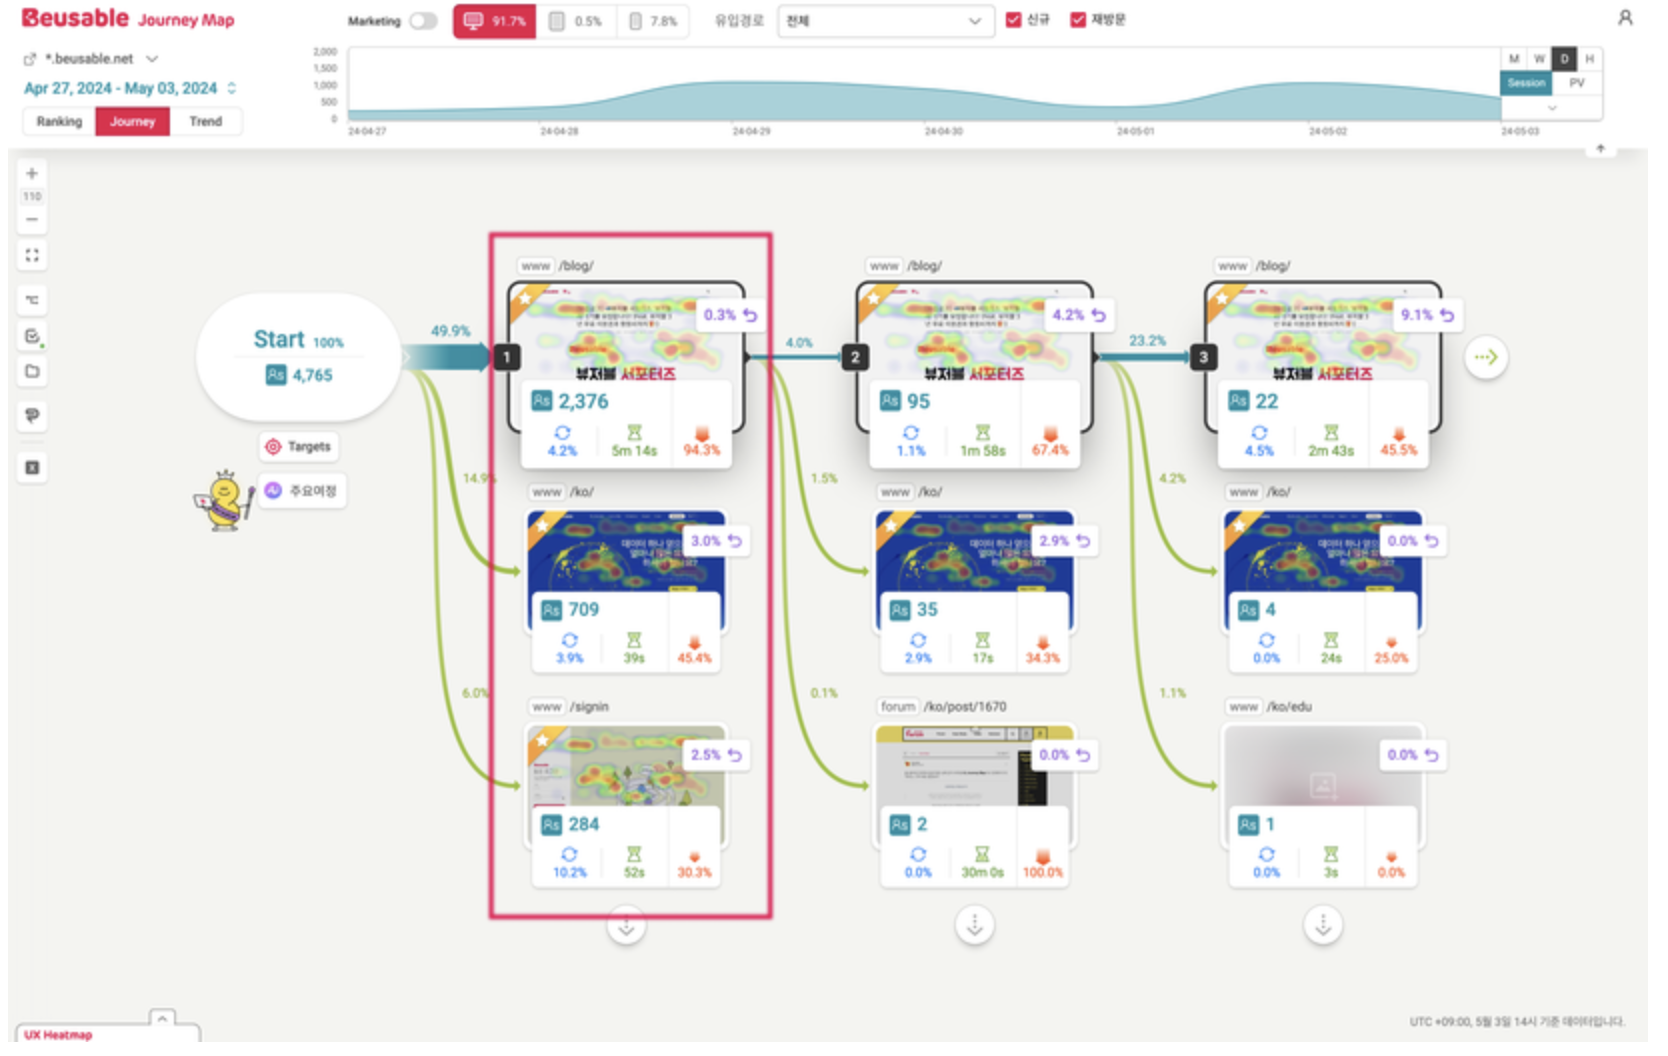
\includegraphics{img/fig20.png}

}

\caption{Beausable의 고객 여정 분석 화면}

\end{figure}%

(문헌 16)Google marketing platform, ``애널리틱스 기능''
\url{https://marketingplatform.google.com/intl/ko/about/analytics/features/}

(문헌 17) Microsoft, ``Power BI 둘러보기''
\url{https://powerbi.microsoft.com/ko-kr/guidedtour/power-platform/power-bi/2/1}

(문헌 18) Tableau, ``Tableau product''
\url{https://www.tableau.com/ko-kr/products/tableau}

(문헌 19)Beausable, ``Why Beausable'',
\url{https://www.beusable.net/ko/}

\chapter{ch5. Lean UX 프로세스와 데이터 기반
디자인}\label{ch5.-lean-ux-uxd504uxb85cuxc138uxc2a4uxc640-uxb370uxc774uxd130-uxae30uxbc18-uxb514uxc790uxc778}

\section{Lean Design Process의
개념}\label{lean-design-processuxc758-uxac1cuxb150}

목표한 디자인 해결안을 완성하기까지 수행하는 디자인 활동의 내용과 방법,
과정을 정의하는 디자인 프로세스는 디자인의 대상과 사회, 기술적 요구
사항의 변화에 따라 변화하고 있습니다. 현대의 디자인 프로세스는
소프트웨어 기술과의 협업 과정, 비즈니스 방법의 변화에 영향을 받아
애자일(Agile) 디자인 프로세스, 린(Lean)디자인 프로세스라는 특별한 형식의
디자인 프로세스를 적용하는 사례가 많습니다.

`Lean'이라는 단어가 `기대다', `의지하다'라는 의미가 있고 `군살이 없는'
이라는 의미도 있으므로, 린 디자인 프로세스는 편하게 기대어서 하는
디자인, 군살없이 날씬하게 진행하는 디자인 프로세스라는 의미로 생각해볼
수 있습니다. 결국 이 말은 디자인을 하는데, 쓸데 없는 일을 과하게 하지
않고, 시간과 비용의 효율을 추구하는 디자인 방법이라는 뜻입니다. 제품이나
서비스의 생산 주기가 짧고, 소규모 조직으로도 서비스 운영이 가능해진 현대
산업계의 특징을 반영하여 빠른 시간에 적은 인원을 가지고, 꼭 필요한
작업만을 효율적으로 해서 디자인을 수행하는 것이 린 디자인 프로세스의
철학입니다. 이러한 린(Lean) 철학을 UX 디자인 방법론에 가져온 것이 Lean
UX입니다. 그러므로 Lean UX는 UX 디자인의 과정에서 시간과 자원을
효과적으로 사용하여 결과물을 산출하는 방법론이겠죠. UX 디자인 업무가
전통적으로 시간과 조직 역량을 많이 필요로 했던 문제를 해결하고자 한
방법론이라고 하겠습니다. 린 UX는 디자인의 효율화를 추구하는 핵심적인
전략으로 정량 데이터를 적극적으로 활용합니다.

'린 스타트업 실전 UX'라는 책에서 저자(Laura Klein)는 린 UX에 대하여 Lean
비즈니스 환경에 적합한 UX 디자인을 말하는 것으로, 어떤 성과 지표(KPI:
Key Performance Indicator)가 비즈니스를 이끄는지 알아내고, 이러한 지표를
개선하기 위해 해결해야할 고객의 문제가 무엇인지 이해하고(Hypothesis),
고객의 어려움을 개선하는 데 필요한 아이디어를 구현한 다음(MVP: Minimum
Viable Product), 그게 적합한 아이디어인지 검증(A/B testing)하는 것이라고
설명했습니다. (20)

갑자기 낯선 용어들이 많이 나오죠? 괄호 안의 전문 용어들을 빼고 조금 쉽게
서술해 보면 린 UX는 어떤 비즈니스가 잘 되고 있는지를 측정하는 지표 값을
찾고, 이 값을 원하는 목표 값까지 달성하기 위하여 디자인을 수행한 뒤, 그
디자인이 성공했는지를 판단하기 위해 이전 디자인의 지표값과 개선 디자인의
지표값을 비교하여 평가한다는 의미입니다. 내용을 다시 해석해 보면 `지표
값' 이라는 정량 데이터가 있고, 이 데이터를 `목표 값'의 정량 데이터로
변환 시키도록 디자인을 한 뒤, 디자인 개선 후의 `지표 값'이 `목표 값'
수준으로 달성 되었는지를 정량적(통계적)으로 판단한다는 뜻이니,
전체적으로 정량 데이터의 측정과 평가를 중심으로 진행하는 디자인
방법론이네요. 그래서 Lean UX는 결국 데이터에 근거하여 디자인 의사 결정을
수행하는 데이터 기반 디자인 방법론의 하나입니다.

\section{Lean UX에 사용하는 주요
용어들}\label{lean-uxuxc5d0-uxc0acuxc6a9uxd558uxb294-uxc8fcuxc694-uxc6a9uxc5b4uxb4e4}

Lean UX를 수행하기 위하여 이해해야하는 KPI, Hypothesis, MVP, A/B
테스팅의 개념을 아래와 같이 정리하였습니다. 각각의 개념은 이후의 실습
프로젝트를 수행하면서 더 명확하게 이해할 수 있을 것입니다.

\begin{itemize}
\item
  KPI(Key Performance Indicator)

  KPI는 조직이나 프로젝트의 목표 달성 정도를 측정하는 데 사용되는 핵심
  성과 지표를 의미합니다. KPI를 통해 프로젝트의 진행 상황을
  모니터링하고, 목표 달성을 위해 필요한 조치를 취할 수 있습니다. 예를
  들어, 새로운 앱의 성공을 측정하기 위한 KPI로 월간 활성 사용자 수,
  사용자 유지율, 평균 세션 시간 등을 KPI로 설정하고, 이 값으로 앱의
  성과를 평가하고 필요한 개선점을 파악할 수 있습니다.

  주요 특징:

  \begin{enumerate}
  \def\labelenumi{\arabic{enumi}.}
  \tightlist
  \item
    구체적이고 측정 가능함: 명확하고 구체적으로 정의되어야 하며, 수치로
    측정 가능해야 합니다.
  \item
    목표 지향적: 조직이나 프로젝트의 목표와 직접적으로 연결되어 있어야
    합니다.
  \item
    주기적 평가: 정기적으로 평가하여 진행 상황을 모니터링합니다.
  \end{enumerate}
\item
  Hypothesis

  가설은 특정한 질문이나 문제에 대한 예상 답변을 제시하는 것입니다.
  제품이나 기능의 개발 전, 이를 통해 어떤 결과가 나올지를 미리 예측하고
  테스트하는 과정을 의미합니다. Lean UX에서는 가설을 바탕으로 실험을
  진행하고, 그 결과를 통해 제품을 개선합니다. 예를 들어, ``앱의 새로운
  알림 기능을 제공하면 앱을 더 자주 사용할 것이다''라는 가설을 세우고,
  이를 테스트하기 위해 새로운 알림 기능을 출시한 후 사용자 반응을
  분석합니다.

  주요 특징:

  \begin{enumerate}
  \def\labelenumi{\arabic{enumi}.}
  \tightlist
  \item
    명확한 진술: 가설은 구체적이고 명확하게 진술되어야 합니다.
  \item
    검증 가능: 실험을 통해 가설의 진위 여부를 확인할 수 있어야 합니다.
  \item
    피드백 중심: 사용자 피드백을 통해 가설을 검증하고 개선.
  \end{enumerate}
\item
  MVP(Minimum Viable Product)

  MVP란 제품 개발 과정에서 최소한의 기능만을 갖춘 제품을 의미합니다. 이
  제품은 사용자에게 실질적인 가치를 제공하면서도 개발에 소요되는 시간과
  비용을 최소화하는 것이 목적입니다. MVP를 통해 빠르게 시장에 제품을
  출시하고, 사용자로부터 피드백을 받아 제품을 개선해 나갈 수 있습니다.

  주요 특징:

  \begin{enumerate}
  \def\labelenumi{\arabic{enumi}.}
  \tightlist
  \item
    최소한의 기능: 제품의 핵심 기능만 포함.
  \item
    빠른 출시: 개발 시간을 줄여 빠르게 시장에 출시.
  \item
    사용자 피드백: 실제 사용자로부터 피드백을 받아 제품을 개선.
  \end{enumerate}
\item
  A/B 테스팅

  A/B 테스트는 디자인의 구현 과정에서 화면이나 기능을 여러 버전으로
  만들어서 서로 다른 사용자 그룹에 각기 다른 것을 보여주고 어떤 버전이
  최선의 지표를 이끌어 내는지 찾아내는 기법입니다. A/B 테스트의 목적은
  통계적으로 의미있는 데이터를 활용해서 사업적 중요성(KPI)을 기준으로
  제품에 관련된 더 나은 의사결정을 하려는 것입니다. 예를 들어,
  웹사이트의 버튼 색상을 A는 파란색, B는 빨간색으로 설정하여 어떤 색상이
  더 많은 클릭을 유도하는지 테스트합니다.

  주요 특징:

  \begin{enumerate}
  \def\labelenumi{\arabic{enumi}.}
  \tightlist
  \item
    두 가지 버전: A 버전과 B 버전, 두 가지 버전으로 나눔.
  \item
    실험군과 통제군: 사용자 그룹을 나눠 각각 다른 버전을 사용하게 함.
  \item
    성과 측정: 각 버전의 성과를 비교하여 더 나은 쪽을 선택.
  \end{enumerate}
\end{itemize}

\section{Lean UX Process Diagram (Learn\textgreater{} Build
\textgreater{} Measure \textgreater{} Learn \textgreater 의
반복)}\label{lean-ux-process-diagram-learn-build-measure-learn-uxc758-uxbc18uxbcf5}

데이터를 중심으로 의사결정을 하는 린 UX의 또 하나의 중요한 특징은
반복적인 수행 과정입니다.

데이터를 통하여 알게된(Learn) 인사이트를 가지고 KPI를 개선하는
아이디어(가설)를 내고, 이것을 MVP로 개발하여(Build) 아이디어가 잘
작동하는지는 검증(Measure)하고, 검증 데이터를 바탕으로(Learn) 다시
개선안을 내고, 이것을 MVP로 개발하여(Build) 아이디어가 잘 작동하는지는
검증(Measure)하는 반복적인 과정을 원하는 수준의 KPI에 도달할 때까지
반복하여 진행합니다. 최종 디자인 목표가 달성될 때까지
Learn\textgreater{} Build \textgreater{} Measure \textgreater{} Learn
\textgreater 의 과정은 반복됩니다. 이 과정을 그림으로 표현하면 {[}그림
22{]}과 같습니다.

애플은 앱 디자인 프로세스를 설명할 때 같은 개념을 Think\textgreater{}
Make\textgreater{} Check\textgreater{} Think의 반복적 프로세스로
설명했습니다.

\begin{figure}[H]

{\centering 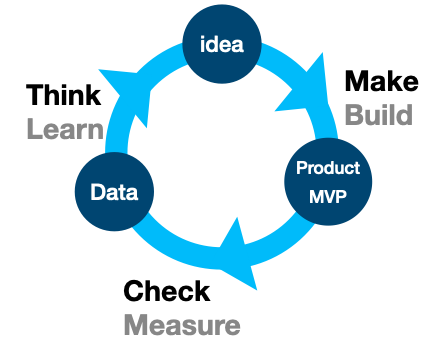
\includegraphics[width=3.875in,height=\textheight]{img/fig21.png}

}

\caption{순환적이고, 반복적인 Lean UX 디자인 프로세스}

\end{figure}%

\begin{itemize}
\tightlist
\item
  다음은 참고도서의 저자인 Laura Klein이 Lean UX에 대하여 설명하는
  영상입니다.(21)
\end{itemize}

\url{https://www.youtube.com/watch?v=7NkMm5WefBA}

우리는 Lean UX의 디자인 프로세스인 Leran \textgreater{} Build
\textgreater{} Measure \textgreater{} Learn의 단계를 따라서 실습 과제를
수행하게 됩니다. 그럼 다음 장에서는 Lean UX의 과정을 따라서 데이터 기반
디자인 방법을 실습해 볼까요?

(문헌 20) 로라 클라인, (김수영, 박기석 역), 『린 스타트업 실전 UX』,
한빛미디어,(2014)

(문헌 21) Google Developers, ``UXD: What is Lean UX?'',
\url{https://www.youtube.com/watch?v=7NkMm5WefBA}

\part{\textbf{part 3. 기존 디자인(A 디자인) 리서치와 개선 디자인(B
디자인) 제안}}

\chapter*{part 3. 기존 디자인(A 디자인)리서치와 개선 디자인(B 디자인)
제안}\label{part-3.-uxae30uxc874-uxb514uxc790uxc778a-uxb514uxc790uxc778uxb9acuxc11cuxce58uxc640-uxac1cuxc120-uxb514uxc790uxc778b-uxb514uxc790uxc778-uxc81cuxc548}
\addcontentsline{toc}{chapter}{part 3. 기존 디자인(A 디자인)리서치와
개선 디자인(B 디자인) 제안}

\markboth{part 3. 기존 디자인(A 디자인)리서치와 개선 디자인(B 디자인)
제안}{part 3. 기존 디자인(A 디자인)리서치와 개선 디자인(B 디자인) 제안}

이번 단원은 실습 프로젝트의 디자인 부분을 수행하는 단원입니다. 각 실습
과제들을 통하여 실습 프로젝트의 주제를 선정하고, 주제에 대한 디자인
리서치를 데이터 기반 디자인의 방법을 사용하여 수행하고, 디자인
인사이트와 문제의 구조를 도출하고, 디자인 개선의 목표인 KPI를 설정하고,
KPI의 목표를 만족하는 디자인 해결안을 완성하여 A/B 테스팅 준비를
마칩니다. 이번 단원을 통하여 여러분은 데이터 기반 디자인 방법론을
사용하여 앱 서비스의 디자인 실습을 진행하는 주요 활동들을 전반적으로
경험할 수 있습니다. 좋은 디자인이 나와야 디자인을 검증할 때 보람이
있겠죠. 실습 프로젝트의 여정을 시작해 봅시다.

\href{ch1.\%20실습과제의\%20디자인\%20프로세스,\%20주제\%20선정.qmd}{ch1.
실습과제의 디자인 프로세스, 주제 선정}

\href{ch2.\%20데이터\%20큐레이션과\%20EDA,\%20디자인\%20인사이트.qmd}{ch2.
데이터 큐레이션과 EDA, 디자인 인사이트}

\href{ch3.\%20디자인\%20문제의\%20구조와\%20KPI.qmd}{ch3. 디자인 문제의
구조와 KPI(Key Performance Indicator)}

\href{ch4.\%20Design\%20Concept\%20&\%20MVP(Minimum\%20Viable\%20Product)\%20Design.qmd}{ch4.
Design Concept \& MVP(Minimum Viable Product) Design}

\chapter{ch1. 실습과제의 디자인 프로세스, 주제
선정}\label{ch1.-uxc2e4uxc2b5uxacfcuxc81cuxc758-uxb514uxc790uxc778-uxd504uxb85cuxc138uxc2a4-uxc8fcuxc81c-uxc120uxc815}

\section{실습 과제의 개요 및 디자인
프로세스}\label{uxc2e4uxc2b5-uxacfcuxc81cuxc758-uxac1cuxc694-uxbc0f-uxb514uxc790uxc778-uxd504uxb85cuxc138uxc2a4}

지금까지 이론적으로 공부한 데이터 기반 디자인 개념을 실습 프로젝트를
통하여 몸에 익혀봅시다. 우리가 진행할 실습 프로젝트는 관심 주제의
데이터를 선택하여 데이터를 해석하고, 해당 데이터 인사이트를 디자인에
반영할 서비스(기존 디자인, A디자인)를 선정한 뒤, 이 서비스를 데이터 기반
디자인 방법론을 통하여 개선 디자인(B 디자인)으로 제안하고, 개선 여부를
A/B 테스팅으로 검증하는 과제입니다. 개선 디자인에서 개선되지 못한
부분들은 다시 업데이트한 디자인(최종 디자인, B' 디자인)을 제안하며
과제를 마무리합니다.

앞으로 우리는 A 디자인, B 디자인, B' 디자인이라는 용어를 매우 자주
사용하게 될텐데요, A 디자인은 타겟 서비스, 즉 우리가 새로 디자인할
서비스의 기존 디자인, 현재 운영중인 디자인을 말합니다. 우리는 데이터
기반 디자인 방법론으로 A 디자인의 문제들을 연구하여 새로운 B 디자인을
해결안으로 제안할 예정입니다. 그리고 B' 디자인은 A, B 디자인에 대한
디자인 개선 여부를 A/B 테스팅으로 검증한 뒤, 개선되지 않았다고 평가된
부분들에 대하여 디자인 수정한 해결안을 B' 디자인으로 지칭할 예정입니다.
B' 디자인에 대하여도 A/B 테스팅을 실시하여 개선 여부를 검증하는 과정을
반복적으로 수행하여 지속적으로 서비스를 개선해 나가야하지만, 한 학기의
제한된 시간 여건에서 B' 디자인을 제안하는 것으로 학기 과제를 마치게
됩니다.

실습 과제의 진행 프로세스는 {[}그림 22{]}와 같이 더블 다이아몬드 디자인
프로세스와 린 UX 디자인 프로세스의 융합으로 진행됩니다.

실습 과제의 내용을 주 별 활동 단위로 나누어 정리하면 다음과 같습니다.

\begin{itemize}
\tightlist
\item
  먼저 관심 데이터와 타겟 서비스를 선정해서 관련 데이터를 조사 분석하여
  데이터 인사이트를 도출하고,
\item
  또 한 방향으로는 타겟 서비스에 대한 디자인 분석을 실시하여 디자인
  인사이트를 발견합니다.
\item
  양 방향에서 수집한 디자인 인사이트를 종합하여 타겟 서비스에 대한
  문제의 구조와 KPI를 선정하고
\item
  KPI를 개선할 디자인 콘셉트(가설)를 도출하여
\item
  이를 반영한 개선 디자인과 최소기능제품(MVP)을 제작합니다.
\item
  MVP 디자인에 대한 사용자 반응을 설문 조사하여 A/B 테스트를 실시하고,
  개선 디자인이 목표한 KPI를 달성하였는지 검증합니다.
\item
  목표 KPI를 달성한 디자인 속성을 반영하고, 목표를 달성하지 못한 디자인
  속성은 원인과 해결 방안을 분석, 반영하여 최종 디자인을 완성합니다.
\end{itemize}

\begin{figure}[H]

{\centering 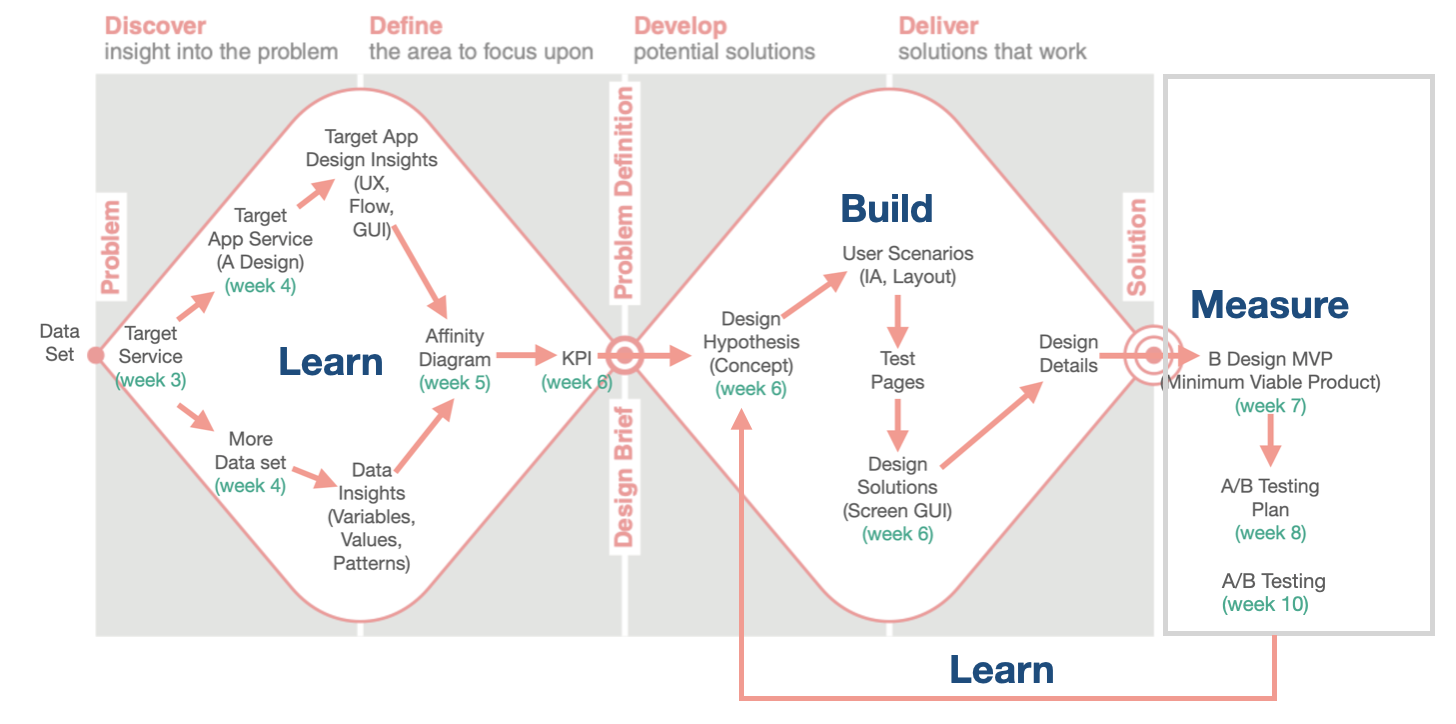
\includegraphics{img/fig22.png}

}

\caption{실습 과제의 디자인 프로세스 : Double Diamond Design Process +
Lean UX Process (실습 주차 표기는 참고 사항이며, 최종 디자인(B'
디자인)의 개발 과정은 개선 디자인(B디자인)의 개발 과정을 반복함.)}

\end{figure}%

이제 부터는 위의 디자인 프로세스를 차근 차근 따라가면서 실습과 이론을
병행하여 설명하도록 하겠습니다. 수업에서 프로젝트 조 구성 3인 1조를
기본으로 하고 있으며, 실습 과제를 주 단위로 수행하고 있습니다.

\section{프로젝트 주제
선정}\label{uxd504uxb85cuxc81duxd2b8-uxc8fcuxc81c-uxc120uxc815}

일반적으로 디자인의 프로젝트를 시작할 때는 먼저 프로젝트의 주제가
정해지고, 이에 대한 데이터 리서치를 실시하는게 정상적인 방법일 것입니다.
특정 프로젝트의 주제와 관련한 데이터를 쉽게 수집할 수 있다면, 이렇게
하는 것이 맞지만, 우리는 학교에서 실습 과제를 수행하는 상황이라서, 알고
싶은 주제의 데이터를 직접 수집하는 것이 어렵습니다. 보통 기업 서비스와
관련된 데이터는 공개 되지 않지요. 또 관련 데이터를 수집한 자료가 아예
없거나, 짧은 시간에 충분한 규모의 데이터를 직접 수집하는 것이 불가능한
경우가 대부분입니다. 데이터 기반 디자인을 하기위한 데이터가 확보가 쉽지
않은 것입니다.

그래서 우리 실습에서는 순서를 바꾸어, 우리가 수집, 분석 가능하도록
공개된 데이터를 먼저 확보하고, 그 데이터와 관련한 서비스를 프로젝트
주제로 정하여 진행합니다. 그래서 아래와 같은 국내 데이터 제공 서비스들을
둘러보고, 관심있는 주제나 사용자 경험과 연계 가능한 데이터들을 선정하고,
이 데이터의 분석 인사이트가 적용될 수 있는 서비스를 선택하여 타겟
서비스(A 디자인)로 정합니다. 그래서 디자인 프로젝트를 정의하는 프로젝트
선언문을(Project Statement) 조금 나중에 결정하게 됩니다. 주어진 여건에서
데이터 큐레이션을 하기위한 현실적인 실습 방법으로 이해하기 바랍니다.

국내의 공공 데이터 제공 서비스는 통합 데이터 지도, MDIS 마이크로데이터
통합서비스, 서울열린데이터광장 등이 있습니다. 이들 서비스는 직접 분석을
해야하는 원본 데이터(raw data)도 제공하고, 원본 데이터를 분석한 가공
데이터나 시각화 그래프, 정리된 데이터 분석 보고서도 제공하고 있어서,
필요에 따라 다양한 수준의 데이터 가공이 가능합니다. 특히 우리 수업은
데이터 분석 기술을 학습하는 수업이 아니기 때문에 이미 분석된 데이터를
사용하는 비중이 높습니다. 예를들어 결혼과 관련하여 인구 통계 분석
데이터, 혼수 소비 시장 데이터, 신혼 부부를 위한 금융 서비스 데이터들이나
분석 보고서가 수집될 수 있다면 웨딩플래너 서비스를 타겟 앱 서비스로
선정하여 디자인 제안 프로젝트를 진행할 수 있습니다. 앞서의 탐구적 데이터
분석 사례에서 미세먼지 측정 데이터와 날씨 데이터를 확보하여 미세먼지
정보 서비스 앱을 디자인 제안한 것도 같은 맥락입니다.

\begin{itemize}
\tightlist
\item
  데이터 검색 및 관심 데이터 조사를 위한 국내 데이터 서비스들
  (22)(23)(24)
\end{itemize}

\href{https://www.bigdata-map.kr}{통합 데이터지도 - 공공 민간 빅데이터
통합 검색}

\href{https://mdis.kostat.go.kr/index.do}{MDIS 마이크로데이터
통합서비스}

\href{https://data.seoul.go.kr}{서울열린데이터광장}

\section{실습과제 2 : 실습 과제의 타겟 서비스(A 디자인)
제안}\label{uxc2e4uxc2b5uxacfcuxc81c-2-uxc2e4uxc2b5-uxacfcuxc81cuxc758-uxd0c0uxac9f-uxc11cuxbe44uxc2a4a-uxb514uxc790uxc778-uxc81cuxc548}

위에 제시한 공공 데이터 서비스나 보도 자료, 논문 등을 활용하여 관심
데이터 주제를 선정해주세요. 수집한 데이터들을 분석하거나 분석된 자료를
해석하여 어떤 이슈나 인사이트가 발견되는지 수집하고, 발견한 인사이트를
활용할 수 있는 앱 서비스를 제안해주세요. 적절한 앱 서비스를 선정하기
위해 여러 개의 (3가지 이상) 서비스를 비교하여 데이터 리서치와 개선
디자인 제안 실습 과제에 적합한 앱을 제시하기 바랍니다.

수집한 데이터는 자세히 분석할 수 있으면 좋지만, 현재 여건에서 가능한
일부만 진행해도 됩니다. 데이터 수집 및 분석은 다음 과제에서도 2-3주간
지속적으로 추가 진행할 것이므로, 완성도가 부족해도 타겟 서비스를 선정할
수 있을 정도로만 우선 진행합니다.

수집한 데이터(수집 출처, 데이터 형식 포함)와 데이터의 인사이트, 제안하는
기존 서비스(A 서비스)의 내용과 선정 이유를 논리적으로 구성하여 2-3페이지
분량의 제안서를 작성합니다.

\section{실습과제 2 Check
Point!}\label{uxc2e4uxc2b5uxacfcuxc81c-2-check-point}

주제 선정 이후의 실습 과정을 용이하게 하기 위하여 아래의 요소들도
고려하기 바랍니다.

\begin{itemize}
\tightlist
\item
  관심 주제의 콘텐츠/ 서비스 내용을 분석하여 데이터 인사이트를 낼 수
  있는 데이터나 데이터 시각화 자료가 존재해야함. (있다고 가정하면 안됨)
\item
  생각하는 서비스의 내용에 대하여 기존에 출시되어 있는 서비스(A안)가
  존재해야함. A서비스와 B서비스를 합쳐서 기존에 없던 C서비스를 만드는
  프로젝트는 안됨 (A/B 테스트 불가, 서비스 내용이 다르면 디자인을 비교할
  수 없음)
\item
  사회 정책을 개발하거나 홍보하는 주제가 아니라 개인의 사용자 경험(인지,
  의사결정, 행위)을 개선하는 주제여야함. 의견을 묻는 것이 아닌 행동
  변화를 확인하는 주제여야 함.
\item
  타겟 서비스의 내용이나 디자인에 대하여 설문으로 사용자 피드백을 얻는
  것이 가능해야함. 사용자 의견을 얻기 위하여 서비스 경험 시간이 많이
  필요한 서비스는 지양함.(예를 들어 학습 경험은 학습 시간, 러닝 커브가
  필요하여 짧은 시간에 앱 화면을 보는 경험 만으로는 평가가 어려움)
\item
  어떻게 서비스를 테스트 할 것인가에 대한 고려가 필요함. 외국인 대상의
  서비스면 외국인 대상으로, 아동 대상의 서비스면 아동 대상으로 테스트
  해야하므로, 테스트를 위하여 60명 이상의 평가 인원 참여가(A테스트 30명,
  B테스트 30명) 가능한 주제를 선택함. 평가 참여 인원은 많을수록 좋음.
\end{itemize}

(문헌22) 통합 데이터지도-공공 민간 빅데이터 통합검색
\url{https://www.bigdata-map.or}

(문헌23) MDIS 마이크로데이터 통합서비스 \url{https://mdis.kostat.go.kr}

(문헌24) 서울열린데이터광장 \url{https://data.seoul.go.kr}

\chapter{ch2. 데이터 큐레이션과 EDA, 디자인
인사이트}\label{ch2.-uxb370uxc774uxd130-uxd050uxb808uxc774uxc158uxacfc-eda-uxb514uxc790uxc778-uxc778uxc0acuxc774uxd2b8}

\section{데이터 큐레이션의 여러
방법들}\label{uxb370uxc774uxd130-uxd050uxb808uxc774uxc158uxc758-uxc5ecuxb7ec-uxbc29uxbc95uxb4e4}

데이터 큐레이션(Data Curation)이란 프로젝트에 필요한 데이터를 선정하고
수집하거나 생성하는 데이터 관리의 과정을 통하여 데이터의 가치를 높이는
행위를 말합니다.(25) 즉, 우리가 분석하고, 이해하고자 하는 대상인
데이터를 확보하는 행위인데요, 데이터 확보의 방법은 기존에 존재하는
데이터를 찾아서 수집하는 방법과 기존에 없던 데이터를 생성하는 두 가지
방법이 있고, 프로젝트의 성격에 따라 두 방법 중에 적절한 방법을
선택하거나 두 방법을 동시에 사용하기도 합니다.

\section{1) 기존의 데이터를 수집하여 큐레이션하는
경우}\label{uxae30uxc874uxc758-uxb370uxc774uxd130uxb97c-uxc218uxc9d1uxd558uxc5ec-uxd050uxb808uxc774uxc158uxd558uxb294-uxacbduxc6b0}

예를 들어 기존의 서비스에 대한 설문 조사, 시장 자료, 웹/앱 서비스 로그
기록, SNS 데이터, IoT 센서 데이터 등이 존재한다면, 이들을 수집할 수
있고, 이미 수집되어 있는 데이터의 확보가 가능하다면 가장 편리한 데이터
큐레이션 방법이겠으나, 많은 경우 원하는 데이터가 내 필요에 맞게 정리되어
있는 경우는 없습니다. 그러므로 내 필요에 적합한 데이터가 가공된 형태로
존재하지 않아도, 여러 관련 데이터를 수집하고 이들을 가공하여 필요한
형태로 재구성하는 경우가 더 많습니다. 또 웹이나 앱 형태의 디지털
서비스들은 서비스 관련 데이터를 실시간으로 확인하거나, 지속적으로
데이터를 축적하고 특정 변수를 모니터하는 것이 가능합니다. 이런 경우는
서비스를 모니터링하기 적합한 데이터 대시보드를 구성해놓고, 관찰 주기나
필요 시점에 따라 바로 데이터 상황을 확인할 수 있는 장점이 있고, 대부분의
상용화된 디지털 서비스는 이러한 데이터 모니터링 시스템을 갖추고
있습니다. 데이터 모니터링 시스템이 있는 경우에는 데이터 분석과 디자인
테스팅을 매우 효과적으로 반복 수행할 수 있습니다. 린 UX를 적용하기 좋은
환경인 것이죠.

이미 수집된 데이터를 찾을 때 다양한 검색 옵션으로 데이터 셋을 찾아볼 수
있는 구글 데이터셋 검색 서비스도 활용해보기 바랍니다.

\begin{itemize}
\tightlist
\item
  구글 데이터셋 검색 (26)
\end{itemize}

\href{https://datasetsearch.research.google.com}{Dataset Search}

\section{2) 데이터를 새로 생성하여 큐레이션 하는
경우}\label{uxb370uxc774uxd130uxb97c-uxc0c8uxb85c-uxc0dduxc131uxd558uxc5ec-uxd050uxb808uxc774uxc158-uxd558uxb294-uxacbduxc6b0}

분석에 필요한 데이터가 없는 경우에는 직접 설문 조사나 사용성 테스트,
시장 분석, 센서 설치 등을 수행하여 필요한 데이터들을 확보합니다. 새로운
프로젝트나 실험을 하는 경우에는 보통 데이터 생성 방법을 통하여 데이터
분석을 실시합니다. 새로 데이터를 생성하는 경우는 프로젝트에 필요한
형식과 내용을 맞추어 데이터를 확보할 수 있는 이상적인 방법이지만
데이터를 생성하는데, 시간과 노력이 많이 요구될 수 있습니다. 특히 장기간,
다량의 데이터를 확보하기 위해서는 많은 자원이 필요하므로, 프로젝트의
여건을 잘 고려하여 데이터 생성 계획을 추진해야 합니다.

최근에는 생성형 인공지능을 사용하여 사용자나 사용 상황에 대한 테스트
데이터를 생성하고, 이 데이터로 출시되지 않은 서비스나 기능을 실험할 수도
있습니다. 다만 인공지능이 생성한 데이터는 가상의 데이터이므로 인공지능
서비스의 성능과 한계를 잘 이해하여 활용해야 합니다.

\section{탐구적 데이터 분석(EDA)의 과정과
방법}\label{uxd0d0uxad6cuxc801-uxb370uxc774uxd130-uxbd84uxc11dedauxc758-uxacfcuxc815uxacfc-uxbc29uxbc95}

이제는 데이터 큐레이션으로 확보한 데이터들을 탐구적 데이터 분석으로
이해할 차례인데요, 앞서의 이론 학습에서 탐구적 데이터 분석은 데이터
시각화 기술을 사용하여 데이터의 특징을 탐지하고 트렌드나 패턴을 확인하여
인사이트를 발견하는 데이터 분석 방법으로 설명했었습니다. 그리고 탐구적
데이터 분석 과정의 특징인 단계적이고 반복적인 수행 과정이 디자인 리서치
과정과 유사하다고 했지요. 이번에는 탐구적 데이터 분석 과정을 단위
행동으로 나누어 실습해보도록 하겠습니다. 아래의 설명들은 데이터 문해력이
갖춰진 경우에는 이해하기 쉽겠으나, 그렇지 않은 경우에는 개념이 어려울 수
있습니다. 원본 데이터를 수집하여 탐구적 데이터 분석을 실시하는 경우에는
아래의 과정들이 모두 필요합니다. 그러나 이미 분석된 그래프나 보고서를
사용하는 경우에는 탐구적 데이터 분석 과정을 참고하여 어떤 시각에서
필요한 디자인 인사이트를 발견할 수 있는지를 이해하고 적용하면 됩니다.

\section{1) 데이터 구조와 변수의
이해}\label{uxb370uxc774uxd130-uxad6cuxc870uxc640-uxbcc0uxc218uxc758-uxc774uxd574}

데이터 구조와 변수를 이해하기 위해 먼저, 확보한 데이터 셋의 형식을
확인하고, 분석에 편리한 형식으로 전환하거나 가공할 필요가 있습니다. csv,
xlsx, json 등 다양한 형식의 데이터가 있고, 데이터 분석도구에 따라 적합한
파일 형식이 있으므로 파일 형식을 확인하고, 필요한 파일 형식으로
변환합니다. 그리고 데이터의 구조와 변수, 값의 형식을 확인합니다. 어떤
변수들이 수집되어 있는지, 변수의 값은 어떤 형식인지(정수, 실수, 문자,
범주, 논리, 시간 값 등)를 확인하고, 분석 용도에 맞게 값의 형식을
정리합니다. 변수 값의 형식에 따라 분석할 수 있는 내용이 달라지므로
데이터 형식의 가공은 매우 중요한 과정입니다. 또 변수들을 통합하거나 값에
따라 변수를 분리하는 작업이 필요할 수 있습니다. 여러 데이터 파일들을
공통 변수를 기준으로 통합하면 새로운 변수 간의 관계를 발견할 수
있습니다. 데이터에서 필요없는 변수를 삭제하고, 가독성을 위해 변수 명을
정리하거나 결측값의 처리 방법을 결정하여 정리하는 것도 효율적인 데이터
분석을 하기 위해 필요한 전처리 과정입니다.

예를들어 앞선 사례의 서울시 미세먼지 측정 데이터는 한 변수로 되어있는
미세먼지 측정값과 초미세먼지 측정값을 두 개의 독립된 변수로 분리하는
작업이 필요했고, 측정소 번호는 숫자가 아닌 문자 형식으로 변환하여 측정소
별로 데이터를 분석할 수 있게 했습니다. 또 미세먼지 측정값과 날씨의
관계를 알기 위하여 분리되어 있던 날씨 데이터와 미세먼지 측정 데이터를
측정 시간을 기준으로 결합하는 작업을 했습니다. 이러한 전처리 작업은
이후의 데이터 분석 작업의 효율을 높이고, 사용 목적에 맞는 데이터 분석을
가능하게 합니다.

\section{2) 변수 별 현황값의 이해 (기술 통계: Descriptive
Statistics)}\label{uxbcc0uxc218-uxbcc4-uxd604uxd669uxac12uxc758-uxc774uxd574-uxae30uxc220-uxd1b5uxacc4-descriptive-statistics}

데이터 가공과 전처리가 완료되었으면, 데이터의 각 변수 별로 값이 어떻게
표현 되는지를 분석합니다. 미세먼지 측정 데이터를 예로 들면, 미세먼지,
초미세먼지의 측정 현황이 어떻게 되는지를 관찰하는 작업입니다. 측정값은
시간이나 측정 장소의 구분에 따라 최소값, 최대값, 평균값, 중간값 등
데이터의 상태를 보여주는 대표값들이 나올 수 있습니다. 또 시간이나 장소의
구분에 따라 값이 어떻게 변화하는지, 평균과 각 값은 얼마나 차이가
나는지를 조사할 수 있습니다. 이렇게 변수 별 현황값의 이해 단계에서는
변수 별로 대표 값과 값의 변동 현황을 조사합니다. 그리고 기술 통계값에서
디자인에 필요한 정보가 발견되면 디자인 인사이트의 목록으로 수집합니다.
예를들어, 미세먼지 측정값의 범위를 알면 서비스에서 사용할 측정 단위와
단위 표현 간격 등을 결정할 수 있습니다. 기술 통계값은 값 자체를 디자인
인사이트로 직접 사용할 수도 있지만, 대표값의 현황으로 부터 다음 단계에서
어떤 시각화 분석이 필요한지와 그래프 표현 방법을 결정하는 단서로도
사용됩니다.

\section{3) 변수의 시각화, 변수 간 시각화를 통한 데이터 변동과 패턴
이해}\label{uxbcc0uxc218uxc758-uxc2dcuxac01uxd654-uxbcc0uxc218-uxac04-uxc2dcuxac01uxd654uxb97c-uxd1b5uxd55c-uxb370uxc774uxd130-uxbcc0uxb3d9uxacfc-uxd328uxd134-uxc774uxd574}

이제는 데이터 현황을 그래프를 통하여 시각적으로 확인해볼 차례입니다.
먼저 앞 단계에서 기술 통계로 알아본 각 변수의 내용을 그래프로 시각화하여
현황을 조사합니다. 데이터 시각화를 통하여 대표값 만으로는 발견하기
어려운 변수값의 변화 추세와 패턴을 직관적으로 알 수 있습니다. 어떤
기준(X축에 표기)에 의하여 값(Y축에 표기)은 비례하여 증가하거나,
감소하거나, 또는 기준 값의 변화와 관련 없을 수 있으며, 범위나 분포의
패턴을 관찰할 수도 있습니다. 이러한 변수 값의 시각화는 표현 기준을 달리
함으로써 다면적으로 변수 값을 이해하게 합니다.

각 변수 별로 시각화를 수행했다면, 이번에는 데이터 셋의 두 변수를
선택하여 관계를 볼 수 있는 그래프를 제작하여 변수 간의 관계를
관찰합니다. 변수 간의 관계는 인과 관계, 상관 관계 등으로 표현됩니다.
예를들어 미세먼지 측정량이 많아지면, 초미세먼지 측정량도 많아지는 지를
그래프로 그려서 조사해볼 수 있습니다. 앞서 사례 연구에서 두 측정량은
전반적으로는 비례 관계에 있지만 비례의 강도는 지역이나 관측 시기에
따라서 다른 것으로 조사되었습니다. 변수 간 시각화를 진행할 때는 기술
통계값이나 각 변수의 시각화 그래프를 바탕으로 논리적인 질문들을
제시해가며, 하나씩 답을 확인해보는 방법으로 수행합니다. 이 과정에서 좋은
디자인 인사이트가 많이 발견될 수 있습니다. 데이터 시각화를 통하여 값의
변동 추세, 값의 관계를 발견하는 활동은 탐구적 데이터 분석 방법론의 핵심
활동이므로, 충분한 시간을 가지고 다면적인 시각화와 해석을 여러 번
진행하기를 권합니다. 앞서 소개한 BI(Business Intelignece) 서비스들을
활용하면, 기본적인 데이터 시각화를 쉽게, 또는 자동적으로 수행할 수
있습니다. 최근의 서비스들은 인공지능 기술을 도입해서 해석도 자동으로
생성해줍니다. 하지만 제안된 해석을 그대로 사용할 지, 다른 관점을
반영하여 재해석 할지는 디자이너의 몫이므로 제안 내용을 잘 판단하고,
데이터 분석 과정을 관리할 수 있는 역량을 가지고 BI 서비스를
사용해야합니다.

\section{실습과제 3: 데이터 큐레이션과
EDA}\label{uxc2e4uxc2b5uxacfcuxc81c-3-uxb370uxc774uxd130-uxd050uxb808uxc774uxc158uxacfc-eda}

실습 과제 2에서 타겟 서비스(A 디자인)를 결정한 상태이므로, 이제는 좀 더
구체적인 데이터 큐레이션과 탐구적 데이터 분석을 시행해보겠습니다.

\begin{itemize}
\tightlist
\item
  먼저, 타겟 서비스가 정해졌으니, 우리의 실습 과제를 명확하게 정의하는
  프로젝트 선언문(Project Statement)을 작성합니다. 실습 과제의 내용을 한
  문장으로 요약한 프로젝트 선언문에는 서비스의 사용자가 누구이며, 어떤
  사용 상황에 있는지, 서비스의 주요 내용과 가치는 무엇인지를 문장으로
  구성합니다. 본 과제의 특징을 반영하여 다음의 문장 요소를 템플릿으로
  사용하여 작성해도 됩니다.

  \begin{itemize}
  \tightlist
  \item
    Project Statement: (리서치한 데이터 내용의) 데이터 인사이트를
    기반으로 (Target Service) 앱의 (사용자 경험A), (사용자 경험B) 에
    대한 개선 디자인을 제안한다. (+ 제안한 디자인은 A/B 테스트를 통하여
    앱 서비스의 개선 여부를 검증한다.)
  \end{itemize}
\item
  데이터 큐레이션: 기존의 데이터를 검색, 수집하는 방법으로 데이터
  큐레이션을 실시합니다. 타겟 서비스를 선정할 때 분석한 데이터에 더하여,
  타겟 서비스의 사용자와 사용 상황, 서비스 내용을 특정하여 더 많은 관련
  데이터를 수집합니다. 되도록 타겟 서비스와 직접적으로 관련된 데이터를
  수집하는 것이 좋고, 데이터의 수집 시점, 수집 사례 수, 데이터의 신뢰성,
  분석에 적합한 형식 여부 등을 고려하여 데이터를 확보합니다. 수집한
  데이터의 출처와 형식 정보를 함께 기술합니다.
\item
  탐구적 데이터 분석: 이론에서 설명한 탐구적 데이터 분석 기법을 적용하여
  수집된 데이터들을 분석하고 인사이트를 도출합니다. 데이터의 구조,
  변수의 대표값, 변수의 변동 패턴과 관계 패턴이라는 여러 가지 관점에서
  단계적으로 데이터를 분석하고 데이터의 의미를 발견합니다. 이렇게 하여
  발견한 데이터 인사이트들을 목록화 합니다. 인사이트를 얼마나 많이
  도출하는 것이 적절한지는 과제와 데이터의 특징에 따라 다르겠으나,
  적어도 30개 이상의 목록을 권합니다. 다음 단계에서 디자인 문제의 구조를
  구성하기 위해서는 섬세하고, 다양한 관점의 인사이트가 많을수록
  좋습니다. 데이터의 인사이트를 작성할 때는 사용자, 사용 상황, 서비스
  내용과 연계하여 문장을 서술합니다.
\end{itemize}

지금까지 작업한 프로젝트 선언문, 데이터 큐레이션, 탐구적 데이터 분석과
디자인 인사이트 수집을 실시하여 발표자료 형식으로 정리하여 문서화
합니다.

\section{실습과제 3 Check
Point!}\label{uxc2e4uxc2b5uxacfcuxc81c-3-check-point}

데이터 큐레이션과 탐구적 데이터 분석 활동에서 아래의 내용을 고려하여
진행하기 바랍니다.

\begin{itemize}
\tightlist
\item
  서비스 필요성을 설명하는 데이터에 집착하지 말것. 서비스의 필요성은
  이미 전제되어 있으므로 필요성 보다는 서비스의 현황을 이해할 수 있는
  데이터를 수집해야함.
\item
  데이터 신뢰성 확보를 위하여 출처 서술 필요함.
\item
  데이터 분석(리서치) 활동들의 연계성, 인과관계가 중요함.
\item
  수집한 데이터들에 대하여 왜 이 데이터가 필요한지, 데이터를 어떻게 분석
  했는지, 그래서 무엇을 알았는지, 알게된 것은 어떻게 인사이트로
  적용하는지가 공감되도록 분석 보고서를 작성함.
\end{itemize}

\section{실습과제 4: 타겟 서비스(A 디자인) 현황
분석}\label{uxc2e4uxc2b5uxacfcuxc81c-4-uxd0c0uxac9f-uxc11cuxbe44uxc2a4a-uxb514uxc790uxc778-uxd604uxd669-uxbd84uxc11d}

실습과제 3이 타겟 서비스와 관련한 광범위한 데이터 수집과 붆석을 목표로
진행했다면, 실습과제 4는 타겟 서비스의 디자인 현황을 분석하는데
집중합니다. 타겟 서비스는 이미 운영되고 있는 서비스이므로 서비스의 기존
디자인이 존재합니다. 이 디자인에는 콘텐츠와 네비게이션 구조, 제공
서비스(기능), 사용 경로, 화면의 그래픽 요소 및 GUI 디자인, 화면 및 구성
요소들의 인터렉션, 콘텐츠 원고의 작성 스타일 등 여러가지 사용자 경험들이
포함되어 있습니다.

\begin{itemize}
\tightlist
\item
  먼저 여러분이 사용자라고 가정하고, 타겟 앱 서비스가 제공하는 사용자
  경험을 사용 경로를 따라 검토해보며 인사이트를 발견하세요. 그리고
  서비스의 화면 별로도 사용자 경험을 분석하여 인사이트를 도출합니다. 앱
  서비스의 경우 앱을 열고 가장 먼저 만나는 홈 화면, 그리고 가장 자주
  사용하게 될 서비스의 주요 화면에 특히 집중하여 사용자 경험을
  검토합니다. 우리는 모든 디자인 문제를 완벽하게 해결하려는 것이 아니라
  중요한 서비스 목표를 달성하기 위한 디자인을 할 것이므로, 많은 사용자가
  자주 접하는 사용자 경험을 자세히 분석하는 것이 중요합니다.
\item
  타겟 앱 분석은 버튼이나 콘텐츠 레이블(Label) 같이 페이지를 구성하는
  단위 구성요소별로 분석하지 않고, 예를들어 `검색 키워드 제안 받기'와
  같은 사용자 경험의 행동 단위를 따라 분석합니다. 즉 `방문한 장소 검색
  화면에서(경로/화면) 제시된 검색 키워드를 사용할 때(단위 사용자 경험)
  제안 키워드를 수정할 수 없다.'(형용사적/동사적 서술)와 같이 인사이트를
  서술합니다. 만약 디자이너 본인이 타겟 앱의 사용자와 매우 다른
  퍼소나(Persona)의 사용자라면, 적절한 퍼소나를 설정하여 해당 퍼소나의
  사용 상황을 가정하고 분석하는 것이 좋습니다. 예를들어 게임을 좋아하는
  10대 사용자의 퍼소나를 써야한다면 해당 사용자의 특징을 반영하여 사용자
  경험을 검토해야합니다. 실무적으로는 퍼소나에 맞는 실제 사용자를
  대상으로 관찰하는 것이 이상적이지만, 과제 여건에 따라 어려운 경우도
  있으므로, 이런 경우에는 실습과제 3의 사용자 데이터 수집 비중을 높여서
  진행합니다.
\item
  타겟 서비스 현황 분석의 결과는 타겟 서비스의 진행 경로와 화면 구성을
  잘 이해할 수 있도록 시각적 이미지로 현황을 보여주고, 이미지에
  인사이트의 해당 부분을 표기하여 문제의 이해도를 높여줍니다. 콘텐츠
  규모가 크거나, 기능이 많은 경우, 다양한 니즈의 여러 사용자가 존재하는
  경우에는 현황 분석에 더 많은 시간과 노력이 필요합니다. 충분한 시간을
  들여서 자세히 사용자 경험들을 검토하기 바랍니다.
\end{itemize}

이상의 내용을 고려하여 타겟 서비스의 사용자 경험을 분석하고 인사이트를
모아 목록을 작성합니다. 과제에서 수행한 내용은 문서화하여 소통합니다.

다음 단계에서는 실습과제 3, 4를 통하여 얻은 프로젝트의 디자인 인사이트
목록을 사용하여 문제의 구조를 도출하고, 문제의 구조를 바탕으로 KPI를
설정하도록 하겠습니다.

\section{데이터 큐레이션, 탐구적 데이터 분석, 타겟 서비스 분석에서 AI의
활용}\label{uxb370uxc774uxd130-uxd050uxb808uxc774uxc158-uxd0d0uxad6cuxc801-uxb370uxc774uxd130-uxbd84uxc11d-uxd0c0uxac9f-uxc11cuxbe44uxc2a4-uxbd84uxc11duxc5d0uxc11c-aiuxc758-uxd65cuxc6a9}

디자인 리서치 과정에서 인공지능 서비스를 잘 사용하면 작업의 난이도와
효율을 높일 수 있습니다. 인공지능 서비스는 하루가 다르게 발전하고,
새로운 방식이 도입되고 있기 때문에 특정 방법이나 과정을 안내하기는
어렵지만, 실습과제를 수행하면서 인공지능에게 어떤 요청을 하고, 어떤
결과물을 받으면 좋을지를 정리해보겠습니다.

\begin{itemize}
\item
  데이터 큐레이션: 디자인 리서치에 적합한 기존의 데이터를 찾거나
  추천하는 것은 인공지능이 잘 할 수 있는 업무는 아닙니다. 생성형
  인공지능은 환각 현상 문제와 이미 학습된 데이터를 기반으로 응답하는
  문제가 있어서 최신이면서도 정확한 정보를 AI 서비스로 찾아내는 데는
  아직 한계가 있을 수 있습니다. 대신, 데이터를 검색할 때 어떤 데이터
  서비스에서 어떻게 검색 조건을 쓰면 원하는 데이터를 찾을 수 있는지를
  판단하는 데에 활용하는 것이 현실적이라고 봅니다.

  한편, 생성형 AI의 특징은 테스트 데이터를 생성하는 데는 강점이 될 수
  있습니다. 원하는 조건의 퍼소나(persona) 데이터나 사용 시나리오를 다수
  생성하거나, 데이터의 형태(변수와 값, 관측 수)를 정의하고 이에 맞게
  테스트 데이터를 생성하는 일은 편리하게 수행할 수 있으므로, 이를
  이용하여 데이터를 기획하고, 데이터 형식을 검증하는 일에는 적합합니다.
  이 경우에도 인공지능이 생성한 데이터는 현실 데이터가 아니므로,
  데이터의 값을 신뢰할 수는 없습니다.
\item
  탐구적 데이터 분석: 데이터를 가공하거나 분석하고, 그래프로
  시각화하거나, 데이터의 인사이트를 요약하는 것은 인공지능이 잘 하는
  일입니다. 데이터 분석을 수행하는 인공지능 서비스도 많이 나와 있구요.
  어떤 서비스는 데이터만 제공하면 주요 내용에 대한 분석 보고서를
  생성해주기도 합니다. 또 2-4에서 소개한 BI 서비스들은 비즈니스에서
  반복적으로 수집되고, 축적되는 데이터들을 지속적으로 모니터링하고, 문제
  상황을 감지하거나 예측할 수도 있습니다. 그러므로 본인의 업무 상황과
  필요에 적합한 AI 서비스를 선택한다면, 탐구적 데이터 분석 과정은 비교적
  쉽게 진행됩니다. 다만, 탐구적 데이터 분석을 잘 하려면, 디자이너가
  필요한 정보와 분석 방법을 요청하고, 분석 과정을 관리하고, 결과를 검수
  할 수 있는 데이터 문해력과 분석 도구의 사용 능력을 함께 갖춰야합니다.
  데이터 분석 전문가인 인공지능과 소통하고, 협업 과정을 이끌 수 있는
  역량이 필요하다는 것입니다.
\item
  타겟 서비스의 디자인 현황 분석: 최근의 인공지능 서비스들은 디자인
  화면을 제시하면, 유사한 디자인 사례를 검색해주거나, 화면의 디자인 구성
  요소들을 추출하거나, 사용자의 워크플로우를 제안해주는 등, 디자이너의
  수고를 덜어주는 서비스들이 다수 나와 있습니다. 이렇게 분석 작업의
  과정을 지원하는 인공지능 서비스들은 당연히 잘 사용하는 것이 좋겠고,
  타겟 서비스의 디자인 장점과 문제점을 분석 표나 보고서 원고 형태로
  생성할 수 있습니다. 이 경우에는 표나 보고서의 구체적인 형식과 내용
  예시 등을 템플릿으로 제시하여 원하는 내용으로 결과가 정리되도록
  합니다. 이번 연습 과제에는 포함되지 않지만, 사용자 테스트를
  기획하거나, 사용자 테스트 결과 데이터를 분석하는 방법을 실험해보는
  일에도 인공지능을 활용하는 것이 편리합니다.
\end{itemize}

(문헌25) Renee. Miller, ``Big Data Curation'', 20th International
Conference on Management of Data (COMAD), (2014), p.4

(문헌26) Google Dataset Search,
\url{https://datasetsearch.research.google.com}

\chapter{ch3. 디자인 문제의 구조와 KPI(Key Performance
Indicator)}\label{ch3.-uxb514uxc790uxc778-uxbb38uxc81cuxc758-uxad6cuxc870uxc640-kpikey-performance-indicator}

\section{데이터 모델과 디자인 문제의
모델링}\label{uxb370uxc774uxd130-uxbaa8uxb378uxacfc-uxb514uxc790uxc778-uxbb38uxc81cuxc758-uxbaa8uxb378uxb9c1}

눈에 보이지 않거나 너무 복잡해서 이해하기 어려운 어떤 현실을 이해하기
위하여 가상의 모형을 만들어낸 것을 모델이라고 합니다. 가까운 예로 지도
같은 것이 현실에서는 한 눈에 보이지도 않고, 복잡한 지형 지물들 때문에
알아보기 힘든 지리 정보를 목적에 맞게 요약해서 보여주는 모델입니다.
그래프도 값의 현황을 잘 이해할 수 있도록 만든 모델이죠. 이런 관점에서
우리가 시각화한 그래프들은 그 자체로 데이터 모델이라고 할 수 있습니다.
통계적 관점으로는 모델이 구현되는 수식으로 정의되기도 합니다. 데이터
분석으로 도출된 각 그래프나 수식들은 데이터에 대한 부분적 시각으로
현실을 상징합니다.

그런데 이 모델들이 서로 관계성을 가지고 연결되고, 여러 관계들을 한 눈에
보일 수 있도록 종합할 수 있다면, 어떤 가치를 갖게 될까요? 이 종합 모델은
데이터 전체를 상징하는 가상 현실 모델이 될 겁니다. 만약 데이터들이 타겟
프로젝트의 디자인 문제들에 관한 것이라면 디자인 문제의 추상적 모델이
구축됩니다. 디자인 문제의 모델이 있다면 우리는 디자인 문제가 왜
발생하고, 어떤 문제들끼리 관련되어 있는지, 어떤 디자인 문제가 가장
근원적인 문제인지를 알 수 있겠죠. 나아가 근원적인 디자인 문제를 특정하고
해결하는 디자인을 생각해낼 수 있게 됩니다. 디자이너들은 이러한 디자인
문제의 모델을 어피니티 다이어그램을 기반으로 구축해왔습니다. 전 단계에서
데이터의 변수와 값을 통하여 여러 디자인 인사이트들을 발견했다면, 이제는
이들을 종합하여 디자인 문제의 모델을 제작합니다.

디자인 문제의 모델은 지금까지 해왔던 것처럼 디자이너의 판단과 사고
과정을 통하여 구축할 수도 있고, 통계적 모델링 방법으로 구축할 수도
있습니다. 디자인 문제의 모델 또한 한 가지의 궁극적인 모델 보다는 여러
목적 별로 구성 시각을 달리하여 구축하는 것이 더 현실적이므로, 기술적
모델링 기법도 쓰고, 인간적 모델링 기법도 사용하여 다양한 모델링 작업을
해보는 것이 좋습니다. 데이터 과학의 방법론으로 디자인 문제를 모델링하는
기술은 디자인 방법론의 연구 관점에서 아직 연구가 더 필요한 영역입니다.
디자인 문제의 모델링 기법에 대하여 앞으로 더 좋은 방법의 연구가
진행되기를 기대하며, 우리의 실습 과제에서는 디자이너들이 기존에
작업해왔던대로 데이터에서 수집한 디자인 인사이트 목록을 사용한 어피니티
다이어그램 제작을 통하여 문제의 구조를 이해합니다. 이제 실습 과제를
통하여 문제의 구조를 도출해보겠습니다.

\section{실습과제 5: 디자인 문제의 구조
도출}\label{uxc2e4uxc2b5uxacfcuxc81c-5-uxb514uxc790uxc778-uxbb38uxc81cuxc758-uxad6cuxc870-uxb3c4uxcd9c}

디자인 인사이트 목록, 어피니티 그룹핑의 과정과 방법 서술, 완성된
어피니티 다이어그램을 정리하여 문서로 작성합니다.

\begin{itemize}
\item
  디자인 인사이트 목록의 완성

  앞서의 실습과제 3, 4에서 각 과제의 최종 산출물을 디자인 인사이트의
  목록으로 작성하였습니다. 실습과제 3에서 얻은 디자인 인사이트들은
  프로젝트의 사용자나 사용 상황, 시장 관련 데이터의 개별 분석에서 나온
  사실이나 판단 내용일 것입니다. 또한 실습과제 4의 타겟 서비스를
  분석하여 얻은 디자인 인사이트들도 포함되어 있을 것입니다. 이 모든
  인사이트들을 하나의 목록으로 모으고, 문장 내용이 중복되지 않게
  정리합니다. 어피니티 다이어그램이 의미있는 구조를 갖추어 나오려면
  어피니티가 많을 수록 좋고, 적어도 100여개 이상의 인사이트들을 수집하는
  것이 좋습니다.
\item
  1, 2차 어피니티 그룹핑과 AI 서비스의 사용

  어피니티(affinity)는 요소들 상호 간의 강한 연관성이나 끌림을 의미하는
  용어입니다. 즉 어티니티 다이어그램은 어피니티의 대상인 인사이트들을
  연관성이 높은 것끼리 묶어 의미의 관계를 만들어내는 작업입니다.
  이론적으로는 하나 하나의 인사이트 문장들을 서로 비교하여 구축을
  해나가야 하지만 많은 수 의 어피니티를 1:1로 비교하는 것은 시간과
  노력이 많이 들게 되므로, 우선 1차적으로 내용의 유사성을 가진
  인사이트들을 10\textasciitilde20개의 소그룹으로 그룹핑하고, 이
  소그룹들을 다시 2차 그룹핑을 실시하여 5\textasciitilde10개의 중그룹을
  만듭니다.

  어피니티 그룹핑 과정은 생성형 인공지능 서비스를 사용하여 인사이트
  문장들을 재구성하면 편리합니다. 생성형 인공지능 서비스에서 1, 2차
  그룹핑을 실시하고 각 소그룹과 중그룹을 요약하는 문장을 생성하게
  합니다. 각 그룹의 요약 문장은 해당 그룹의 인사이트를 대표하는 역할을
  하며, 문제의 구조를 이해하는 중요한 요소가 됩니다. 요약 문장의 주어를
  사용자나 사용 상황이 되도록 하여 사용자 경험에 대한 주요 서술을하면,
  향후 사용자 경험의 문제 체계를 이해하기 좋습니다. 이 과정에서 중요한
  점은 그룹핑의 체계나 각 그룹의 주제를 미리 정해 두는 것이 아니라,
  그룹핑을 실시한 뒤 구조를 발견하고, 그룹 내용 요약을 한다는 점입니다.
  어피니티를 구축하는 목적이 우리가 몰랐던 문제의 구조를 발견해내는
  것이므로 미리 틀을 짜놓고 맞춰가면 안됩니다. 특히 디자인의 구성 요소나
  서비스 기능 요소 별로 그룹핑을 하면 안됩니다. 사용자 경험의 문제는
  통합적인 것이라서 단위 디자인 구현 요소를 개별적으로 개선하려고 하면,
  근원적인 문제 해결을 하기 어렵습니다.

  그리고 인공지능이 생성한 그룹핑 내용이 적절한지 반드시 검수하고,
  1차에서 적절하지 않은 부분들은 수정한 뒤, 수정된 내용으로 2차 그룹핑
  작업을 하기 바랍니다. 2차 그룹핑도 내용을 검수하여 적절한 수정을 한
  뒤, 그룹핑의 요약문을 작성하게 합니다. AI 서비스들마다 작업 성능이
  다르므로, 여러 AI 서비스에 같은 작업을 시켜보고, 작업 결과의 장단점을
  판단하여 종합적으로 작업을 진행하는 것이 좋습니다.
\item
  시각화 다이어그램 구성

  완성된 그룹핑 구조와 그룹의 요약문을 가지고 시각적인 다이어그램을
  구성합니다. 다이어그램은 기본적으로 2차의 포함 관계를 가진 인사이트
  그룹들의 트리구조 레이아웃 모델이겠지만, 주제에 따라 트리 구조가 아닌,
  시간 흐름이나 순차적 단계가 보이는 레이아웃이 될 수도 있고, 서로 관련
  없이 독립적인 여러 개의 구조가 만들어질 수도 있습니다. 그러므로 각
  그룹의 요약문을 보고 그룹간의 거리와 위치, 포함 관계를 판단하여
  그룹들의 관계가 가장 잘 표현되는 그래픽 구성과 레이아웃을 적용합니다.
  그리고 다이어그램은 구성하는 시각에 따라서도 여러 모양의 구조가 나올
  수 있으니, 다양한 시각으로 다이어그램 구성 시도를 해보고, 주요 문제
  그룹의 구성, 문제 그룹간 연계 관계, 가장 중요한 문제들을 이해하기 좋은
  구조를 선택하기 바랍니다.

  \begin{figure}[H]

  {\centering 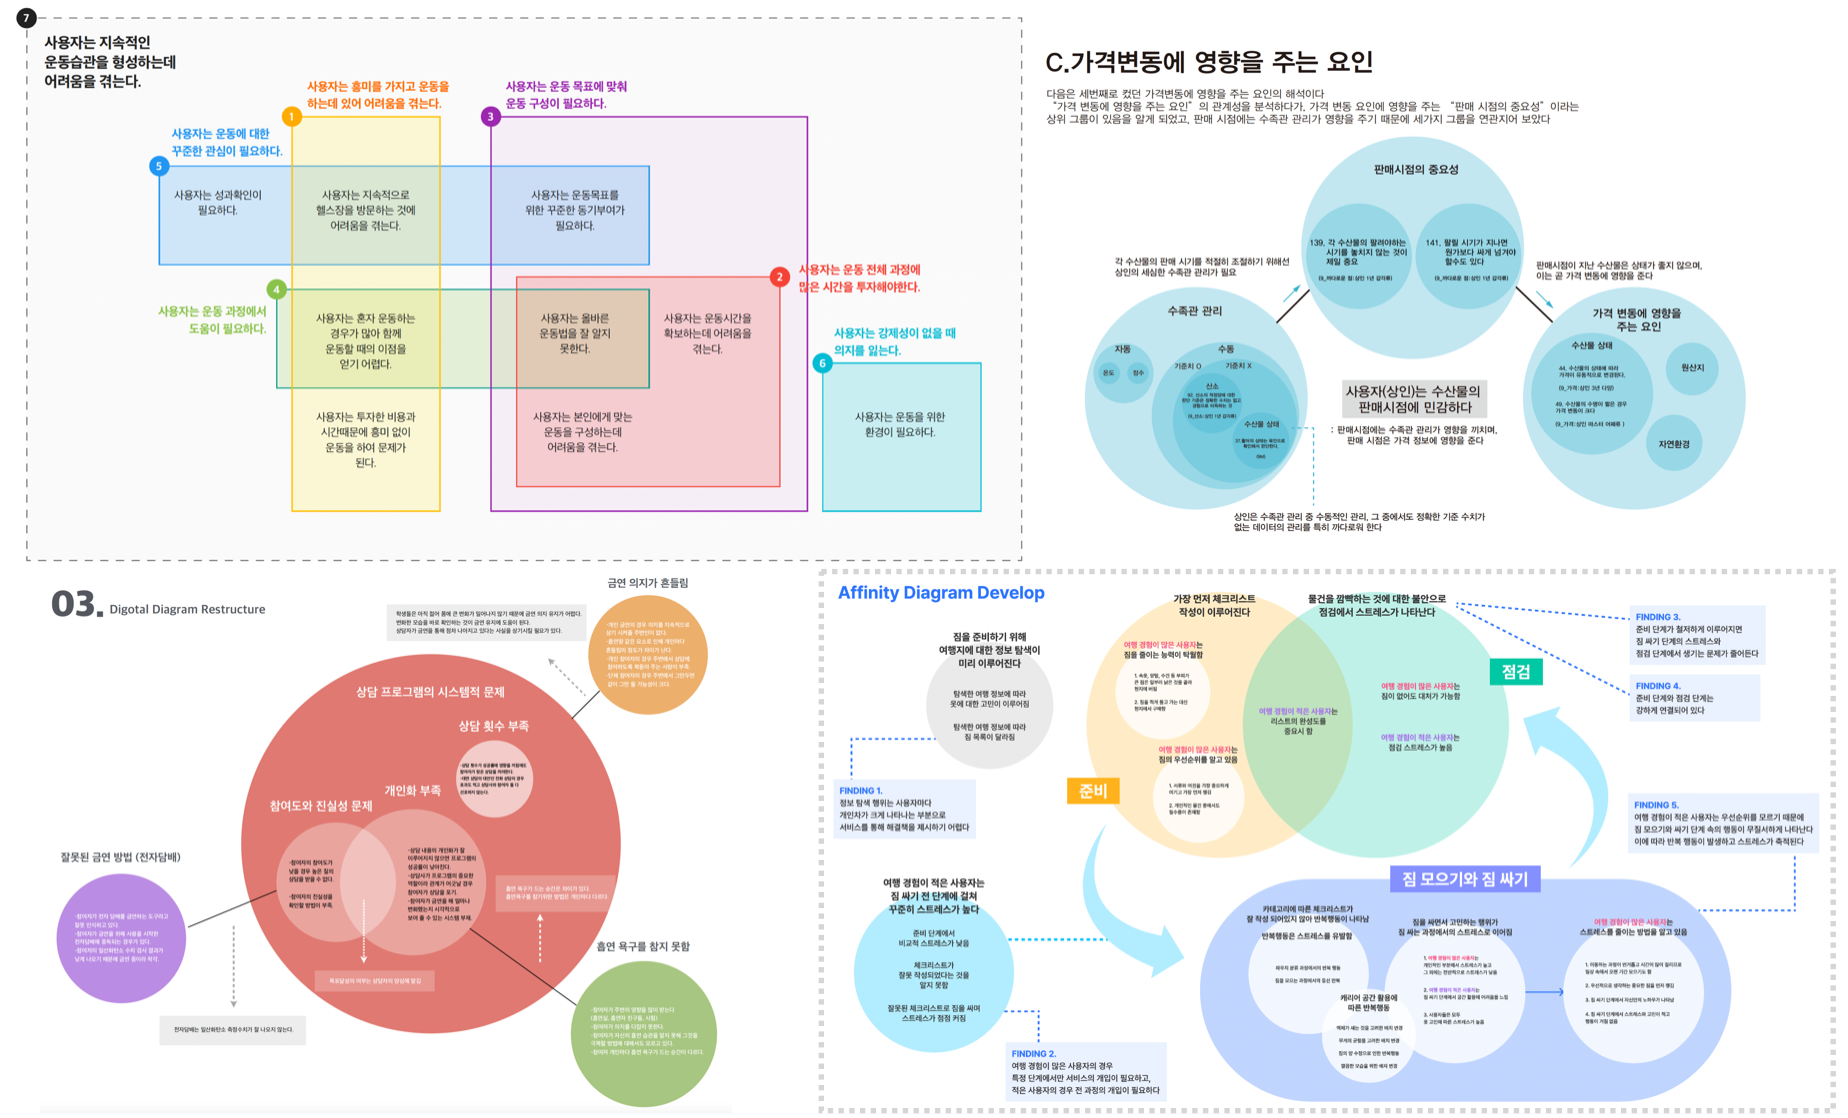
\includegraphics{img/fig23.png}

  }

  \caption{어피니티 다이어그램의 구성 예시들}

  \end{figure}%
\end{itemize}

\section{문제의 구조와 핵심성과지표(KPI, Key Performance Indicator)의
연계}\label{uxbb38uxc81cuxc758-uxad6cuxc870uxc640-uxd575uxc2ecuxc131uxacfcuxc9c0uxd45ckpi-key-performance-indicatoruxc758-uxc5f0uxacc4}

실습과제 5에서 제작한 어피니티 다이어그램을 보면 다른 그룹과의 연결
부분이 많거나 포함된 문제 그룹이 많은 어피니티 그룹들을 발견할 수 있을
것입니다. 이렇게 문제 구조에서 중심을 차지하는 그룹을 주요 문제
그룹이라고 부르고, 그 그룹의 요약문이 사용자 경험의 주요 문제가 됩니다.
우리는 문제의 구조에서 근원적이고, 상위 개념에 있는 사용자 경험을
우선적으로 개선할 것이며, 이 개선 목표를 정량적으로 표현한 값을 KPI (Key
Performance Indicator)라고 합니다.

KPI는 조직의 목표 달성 정도를 측정하기 위한 핵심 성과 지표를 의미하는
용어로, 조직의 성과를 객관적으로 평가하고 향후 개선 방향을 제시하는 데
사용됩니다. 우리의 목표는 사용자 경험의 개선이므로 주요 사용자 경험이
개선되었는지를 확인할 수 있는 정량적인 값이 KPI가 됩니다. 운영중인
디지털 서비스의 경우 사용자 참여도(일일 활성 사용자 수, 월간 활성 사용자
수 등), 단위 기간 당 사용자 유지율, 가입 전환율, 구매 전환율, 사용자
만족도, 신규 사용자 수 등을 일반적인 KPI로 사용합니다. 예시와 같이 KPI는
인원수, 비율, 만족도 점수 등 측정 가능한 숫자 데이터로 설정합니다.

\section{실습과제 6: 주요 사용자 경험의 문제로 부터 KPI
도출하기}\label{uxc2e4uxc2b5uxacfcuxc81c-6-uxc8fcuxc694-uxc0acuxc6a9uxc790-uxacbduxd5d8uxc758-uxbb38uxc81cuxb85c-uxbd80uxd130-kpi-uxb3c4uxcd9cuxd558uxae30}

우리가 실습하는 A/B 테스트 방법과의 연계성을 고려하여 다음 사항들을
반영하여 3\textasciitilde5가지의 KPI를 설정합니다.

\begin{itemize}
\item
  어피니티 다이어그램을 통하여 가장 중요한 문제 그룹 2-3가지를
  선정합니다. 모든 사용자 경험의 문제를 다 해결할 수는 없으므로,
  디자인을 통하여 서비스의 사용자 경험에 가장 큰 변화를 가져올 수 있는
  문제를 선정하는 것이 좋습니다. 이 때 주요 문제 그룹들이 꼭 같은
  수준이나 규모가 아니어도 됩니다. 그리고 UI 문제, 경로 문제, 레이블
  문제 등 앱 구성 요소 수준의 문제는 사용자 경험의 근원적인 문제가
  아니라, 표면적인 문제이므로 주요 문제에서 제외합니다.
\item
  어피니티 다이어그램에서 선정한 주요 문제에 대한 KPI를 도출합니다.
  KPI는 정량 측정 가능한 지표이며, 한 문제 그룹 당 여러 개의 KPI가 있을
  수도 있습니다. 우리는 어피니티 다이어그램의 문제 구조를 보고 KPI를
  정하지만, 실무에서는 개선 요청이 있는 주요 서비스들을 KPI로
  지정합니다. KPI를 정할 때는 측정할 데이터가 어떤 형식의 정량
  데이터이며, 어떻게 수집할지를 함께 고려해야합니다.

  일반적으로 실제 서비스의 사용 데이터 수집이 가능한 경우(사용자 로그
  데이터가 있는 경우)의 KPI는 수집 가능한 데이터 중에 KPI를 선정하거나
  수집된 데이터로 계산할 수 있으면 되지만, 우리 실습과제는 가상
  프로젝트의 특성상 사용자의 실사용 로그 데이터 수집이 불가능하므로,
  사용자 설문 형식으로 수집하고, 측정 가능한 KPI를 설정해야합니다.
  그래서 설문 형식으로 측정 가능한 항목은 주로 사용자의 이해 정도나 사용
  의도, 만족도 등 이므로, 실제 비즈니스의 KPI와는 차이가 있습니다.
  예를들어 지난 실습 과제에서는 뉴스 앱 서비스의 KPI로 뉴스 읽기 경험의
  몰입도, 관심 뉴스 선택 방법의 만족도, 뉴스 콘텐츠의 시각적 만족도를
  설정하였고, 부동산 상권 정보 앱 서비스의 KPI로 상권 분석 데이터의
  유용성, 매물 검색 필터의 설정 만족도, 매물 비교 페이지의 효율성 등을
  설정한 사례가 있습니다.
\item
  생성형 AI 서비스를 활용하여 주요 디자인 문제를 설명해주고, 이에 대한
  KPI를 추천받아 검토해보는 것도 좋은 방법입니다. 다만 우리 실습에서
  KPI를 설문으로 검증해야하므로, 설문으로 측정이 가능한 지표이어야 함을
  반영하여 추천하도록 합니다. 물론 추가적으로 실무에서는 어떻게 KPI를
  설정할지를 예측해 볼 수 있도록 타겟 서비스의 KPI를 추천하고, KPI 측정
  및 검증 방법을 구체적으로 제시하게 하여 비교해보는 것도 좋은 경험이 될
  것입니다.
\end{itemize}

\chapter{ch4. Design Concept \& MVP(Minimum Viable Product)
Design}\label{ch4.-design-concept-mvpminimum-viable-product-design}

\section{디자인 콘셉트와
가설(hypothesis)}\label{uxb514uxc790uxc778-uxcf58uxc149uxd2b8uxc640-uxac00uxc124hypothesis}

실습과제 6에서 KPI를 설정했다면 KPI를 개선할 수 있는 디자인 해결안의
콘셉트를 개발해보겠습니다. UX 디자인 콘셉트는 디자인을 통하여 사용자
경험의 변화가 어떻게 이루어진다는 개념적 서술이며, 디자인 해결안과 달리
디자인 구성 요소를 구체적으로 지정하거나 방법을 제시하지는 않습니다.
디자인 콘셉트를 디자인 해결안으로 구현하는 방법에는 여러 선택지와
가능성이 있기 때문입니다. 앞선 과제의 예시에서 뉴스 읽기 경험의
몰입도라는 KPI를 높이기 위한 디자인 콘셉트로 읽기 경험을 방해하는 앱
알림을 자동으로 끄게할 수도 있고, 몰입도가 증가하도록 폰트와 배경색
변경을 할 수 도 있고, 읽기의 속도에 따라 콘텐츠의 스크롤 인터렉션을
제공하는 콘셉트도 있을 것입니다.

데이터 기반 디자인 방법에서 디자인 콘셉트는 개선 디자인의 효과를 검증을
하는 가설로도 사용됩니다. 가설(Hypothesis)은 어떤 현상이나 문제에 대한
예측이나 추정을 의미합니다. 과학적 실험이나 연구에서 가설은 검증 가능한
진술로, 실험을 통해 옳고 그름을 판단할 수 있습니다. 가설을 세우는 과정은
문제를 명확히 하고, 그에 대한 예측을 구체적으로 기술하는 것입니다. 예를
들어 ``빨간색 버튼이 파란색 버튼보다 클릭 수가 더 많을 것이다.'' 같이
가설을 세울 수 있습니다. 향후 A/B 테스트에서는 설정한 가설이 맞는지를
검증하고, 개선안의 효과를 측정하게 됩니다.

아래의 예시는 Paperless Post라는 e-card 서비스 업체의 데이터 기반 디자인
사례입니다. 이 기업은 상품 수익을 높인다는 KPI를 설정하고, 사용자들이
서비스에서 상품을 구매할 때 사용하는 `Coin'(e-coin)을 사용자가 더 많이
구매하도록 한다는 UX 디자인 콘셉트를 정하였습니다. 그리고 디자인
해결안으로 {[}그림 25{]}의 오른쪽 이미지와 같은 Coin 구매 메뉴를
제안하였습니다. 왼쪽의 기존 Coin 구매 화면과 비교할 때, 많은 수의 Coin을
한꺼번에 구매하면 가격이 더 저렴하다는 것을 메뉴 옵션으로 쉽게 확인하고
더 많은 구매를 유도할 수 있는 디자인입니다.

다음 내용은 예시의 가설(hypothesis)입니다.

``카드 보낼 준비가 된 사용자들은 더 많은 코인을 한꺼번에 구매하는 것이
더 가치 있다고 인식하기 때문에 더 큰 코인 패키지를 구매할 것이다. 이는
평균 주문 금액(Average Order Value)을 증가시키고, 전환율에는 큰 변화가
없으면서도 전체적인 수익을 높이는 결과를 가져올 것이다.``

개선 디자인에 대한 A/B 테스트 결과는 어땠을까요? 개선 디자인에서 수익이
증가했을 뿐 아니라 구매로 이어지는 전환율도 높아지는 좋은 성과를
냈습니다. 가설이 채택된 것입니다. 구매 전환율도 높아진 이유는 개선
디자인을 접한 사용자들이 구매 내용과 본인의 이익에 확신이 생겨서 구매를
더 쉽게 결정했기 때문으로 보입니다.(27)(28)

\begin{figure}[H]

{\centering 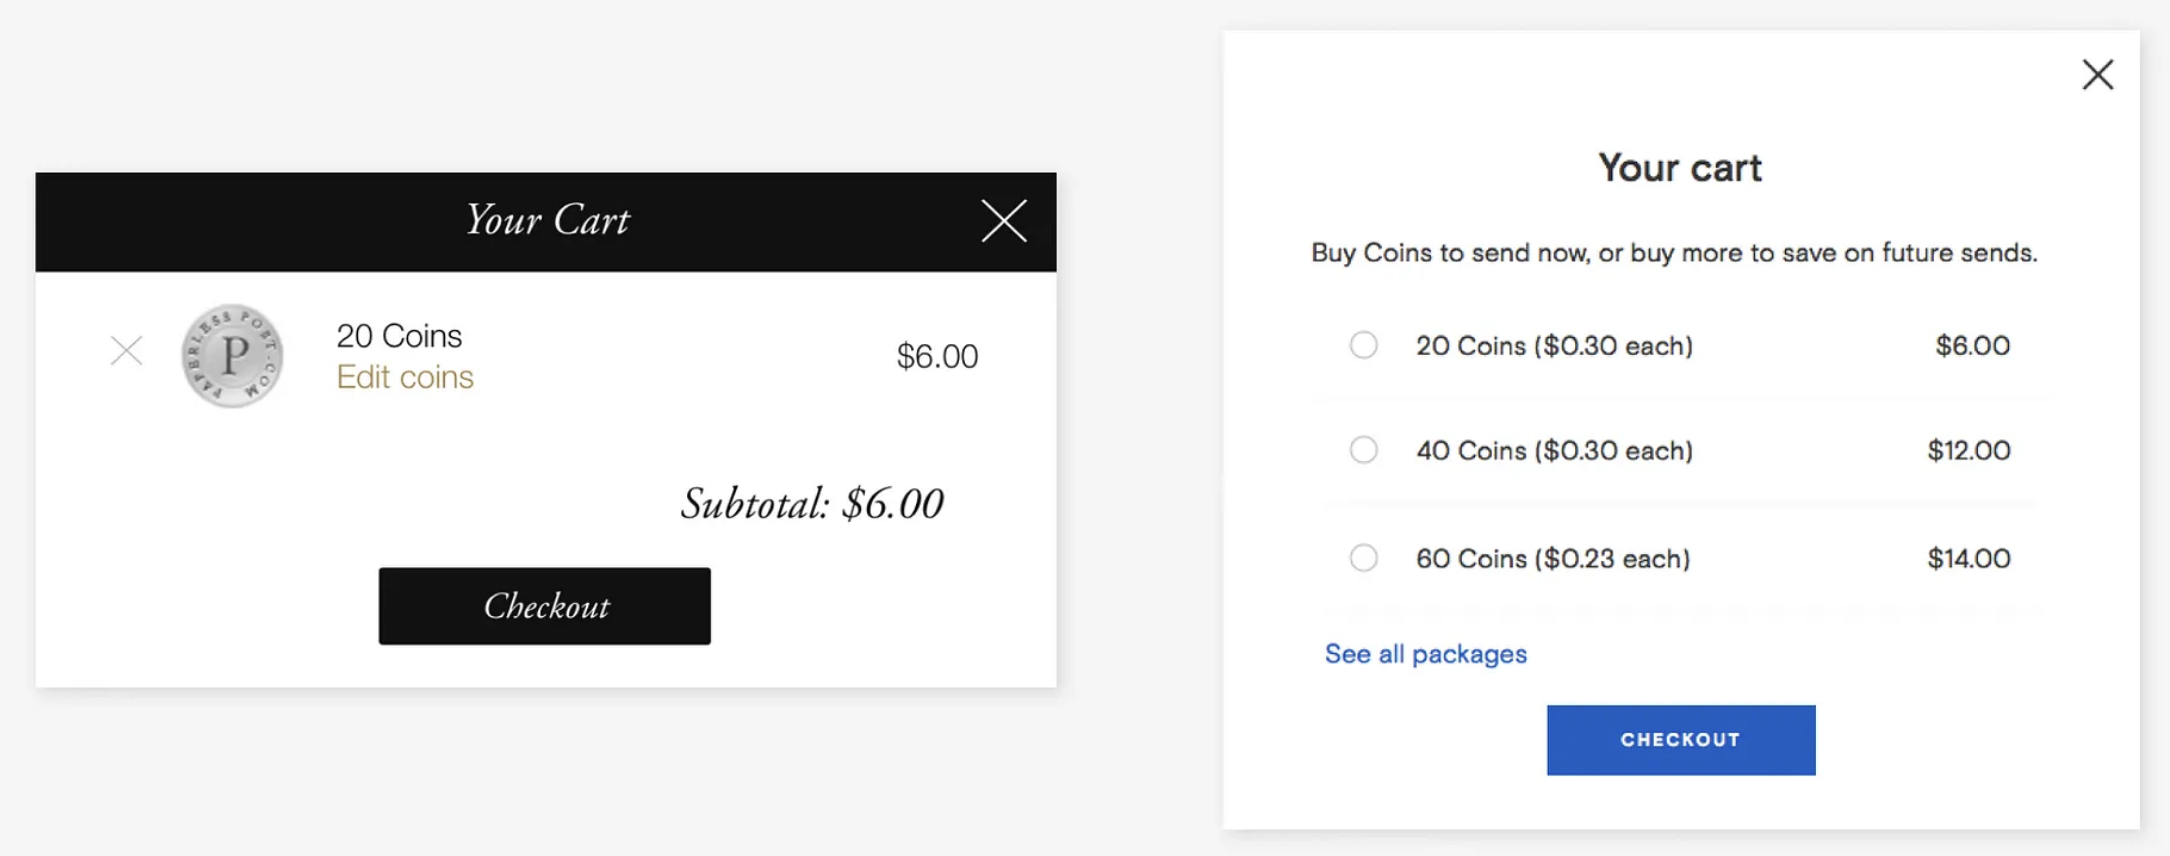
\includegraphics{img/fig24.png}

}

\caption{Paperless Post의 Coin 구매 화면의 기존 디자인(왼쪽, A 디자인)과
개선 디자인(오른쪽, B 디자인)}

\end{figure}%

\href{https://uxdesign.cc/becoming-a-data-aware-designer-1d7614ebc3ed}{Becoming
a data-aware designer}

\href{https://www.paperlesspost.com}{Paperless Post®: Online
Invitations, Greeting Cards, and Flyers}

\section{실습과제 7: 프로젝트의 디자인 콘셉트
개발}\label{uxc2e4uxc2b5uxacfcuxc81c-7-uxd504uxb85cuxc81duxd2b8uxc758-uxb514uxc790uxc778-uxcf58uxc149uxd2b8-uxac1cuxbc1c}

이제 진행중인 실습 프로젝트에서 KPI를 개선할 수 있는 디자인 콘셉트를
개발해보겠습니다. 앞서의 과제에서 우리는 3\textasciitilde5가지의 KPI를
정했기 때문에 각 KPI 마다 디자인 콘셉트가 개발될 수도 있고, 하나의
디자인 콘셉트가 여러 KPI를 개선할 수도 있습니다. 큰 개념의 콘셉트
아래에서 여러 KPI가 자연스럽게 개선된다면 서비스의 사용자 경험이
일관성을 갖게 됩니다. 그러나 두루뭉실한 큰 콘셉트로는 개성있는 디자인
구현이 어려울 수도 있으므로 적정선을 잡아서 디자인 콘셉트를 개발합니다.

\begin{itemize}
\tightlist
\item
  디자인 콘셉트(가설)는 단순하게 '무엇을 디자인 하겠다'가 아니라'어떤
  사용자 경험을 하도록 하여 어떤 KPI를 개선하겠다'가 나와야합니다.
  단순히 GUI 구성 요소의 개선이 아니라 사용자 경험의 KPI가 달라질 수
  있도록 개발합니다.
\item
  앞선 실습과제에서 분석한 프로젝트 주제 관련 데이터에서 발견한 변수
  패턴(각 변수의 대표값, 추세값, 변수간 관계)을 바탕으로 목표 사용자
  경험을 구현해주는(KPI를 개선해주는) 디자인 컨셉을 개발합니다.
\item
  KPI의 개선과 관련 없는 부분은 디자인 콘셉트로 제시하지 않습니다.
  프로젝트의 논리성과 설득력을 높이기 위하여 KPI의 개선에 집중합니다.
  향후 디자인 검증도 KPI의 개선 여부로 측정하므로, 이와 관련 없는 디자인
  콘셉트는 측정되지 않습니다.
\end{itemize}

이상의 항목들을 반영하여 디자인 콘셉트를 개발하고, 해당 KPI와 디자인
콘셉트를 연결하여 표현한 문서를 작성합니다. KPI와 디자인 콘셉트의 연결
내용을 보고 논리적으로 적절하다고 공감할 수 있도록 서술합니다.

\section{디자인 콘셉트를 반영한 최소기능제품(MVP: Minimum Viable
Product)
디자인}\label{uxb514uxc790uxc778-uxcf58uxc149uxd2b8uxb97c-uxbc18uxc601uxd55c-uxcd5cuxc18cuxae30uxb2a5uxc81cuxd488mvp-minimum-viable-product-uxb514uxc790uxc778}

MVP(최소 기능 제품)은 제품 개발 초기 단계에서 최소한의 기능만을 갖춘
버전을 의미합니다. 주요 특징은 다음과 같습니다:

\begin{itemize}
\tightlist
\item
  최소한의 기능: 핵심 기능만을 포함하여 기본적인 사용자 요구를
  충족시킵니다.
\item
  빠른 출시: 제품을 신속하게 시장에 출시하여 사용자의 반응을 얻습니다.
\item
  사용자 피드백: 사용자로부터 피드백을 받아 제품을 개선합니다.
\item
  비용 효율성: 초기 개발 비용과 시간을 절약할 수 있습니다.
\end{itemize}

MVP를 통해 기업은 위험을 최소화하고, 실제 사용자 요구에 맞춰 제품을
지속적으로 발전시킬 수 있습니다. MVP는 실제 사용을 목적으로 하기 보다는
디자인이나 서비스 기능을 검토하는 목적으로 제작 되므로, 적은 투자로
빠르게 제작하여 테스트 목적을 충족해야 합니다. 그래서 모든 기능을 다
구현하지 않고 테스트에 필요한 부분만 구현하며, 안정성, 구동 속도, 데이터
관리와 같이 서비스의 백엔드(Back end)의 세부적인 개발 이슈들은 반영하지
않습니다. 간단하고 빠른 검증을 위하여 실제 개발을 하지 않고,
프로토타입으로 개발하거나, 화면 디자인만 개발하는 경우도 있습니다. 우리
실습 과제에서도 평가할 지표와 관련한 화면 디자인만 개발하여 사용할
예정입니다.

\section{실습과제 8: 기존 A 디자인 화면과 대응되는 개선 디자인 B안의
화면 디자인
개발}\label{uxc2e4uxc2b5uxacfcuxc81c-8-uxae30uxc874-a-uxb514uxc790uxc778-uxd654uxba74uxacfc-uxb300uxc751uxb418uxb294-uxac1cuxc120-uxb514uxc790uxc778-buxc548uxc758-uxd654uxba74-uxb514uxc790uxc778-uxac1cuxbc1c}

이상의 기본 개념 설명에 더하여, 우리 실습과제에서는 A/B 테스트를 사용한
검증 기법을 실습하기에 적합한 MVP를 제작합니다. 데이터 기반 디자인
실습에 적합한 MVP의 조건은 다음과 같습니다.

\begin{itemize}
\tightlist
\item
  우선 타겟 앱 서비스에서 KPI 개선 검증에 필요한 사용자 시나리오를
  선정하고, 시나리오가 적용되는 개별 서비스나 페이지들을 선정합니다.
  테스트할 부분이 기존의 A 디자인의 어떤 부분인지 명확하게
  정의해야합니다. 그래야 기존 디자인과 1:1 대응 비교가 가능한 개선
  디자인 페이지들을 정하여 디자인할 것이기 때문입니다. 그리고 사용자들이
  선정된 화면을 보고 KPI와 관련한 설문 질문에 바로 응답할 수 있는지도
  검토해야 합니다. 예를들어 메뉴를 보고 구매 결정을 하는 화면이라면
  메뉴나 구매 관련 콘텐츠가 적절하게 제공되어 사용자가 구매 결정을
  판단할 수 있는 상태여야 합니다.
\item
  선정한 A 디자인의 각 페이지에 대하여 디자인 콘셉트(가설)를 반영한 개선
  디자인, B 디자인을 개발합니다. A 디자인의 화면과 B 디자인의 화면
  콘텐츠는 내용이 같아야 합니다. A, B 디자인 대응 화면은 사용 상황은
  동일하고, 디자인만 비교되도록 설계하여야 디자인 변화의 영향을 측정할
  수 있습니다. 이렇게 화면 단위의 비교테스트를 진행할 예정이므로,
  서비스의 사용 경로가 매우 다르거나 페이지별로 기능 구성 내용이 매우
  다른 개선 디자인은 평가할 수 없습니다. 개선 내용이 여러가지이고
  복잡하면, 어떤 내용 때문에 개선되었는지를 특정할 수 없어서 테스트의
  검증 효과가 떨어집니다.
\item
  좋은 개선 디자인 개발을 위하여 충분한 디자인 시안 개발과 평가 과정을
  거쳐서 개선안을 완성합니다. 팀원이 여러 명이라면 각자 따로 개선 디자인
  시안을 준비해서 선택지를 넓혀두고, 팀 내 협의를 통하여 최종안을
  도출하는 것이 좋습니다. 디자인 개발은 디자이너에게 가장 중요한 고유
  역량이므로, 좋은 개선안이 나오도록 노력해야하고, 좋은 개선안이 나와야
  테스트에서 가설의 채택 가능성도 높아집니다.
\item
  개선 디자인(B 디자인)의 화면들을 디자인 완료했으면, 기존 디자인(A
  디자인)과 대응하여 이미지 비교가 가능하도록 문서로 정리합니다. 이제
  우리는 A/B 테스트를 실시할 B 디자인(개선 디자인) 개발을 마친 것입니다.
  수고 많으셨습니다.
\end{itemize}

\begin{figure}[H]

{\centering 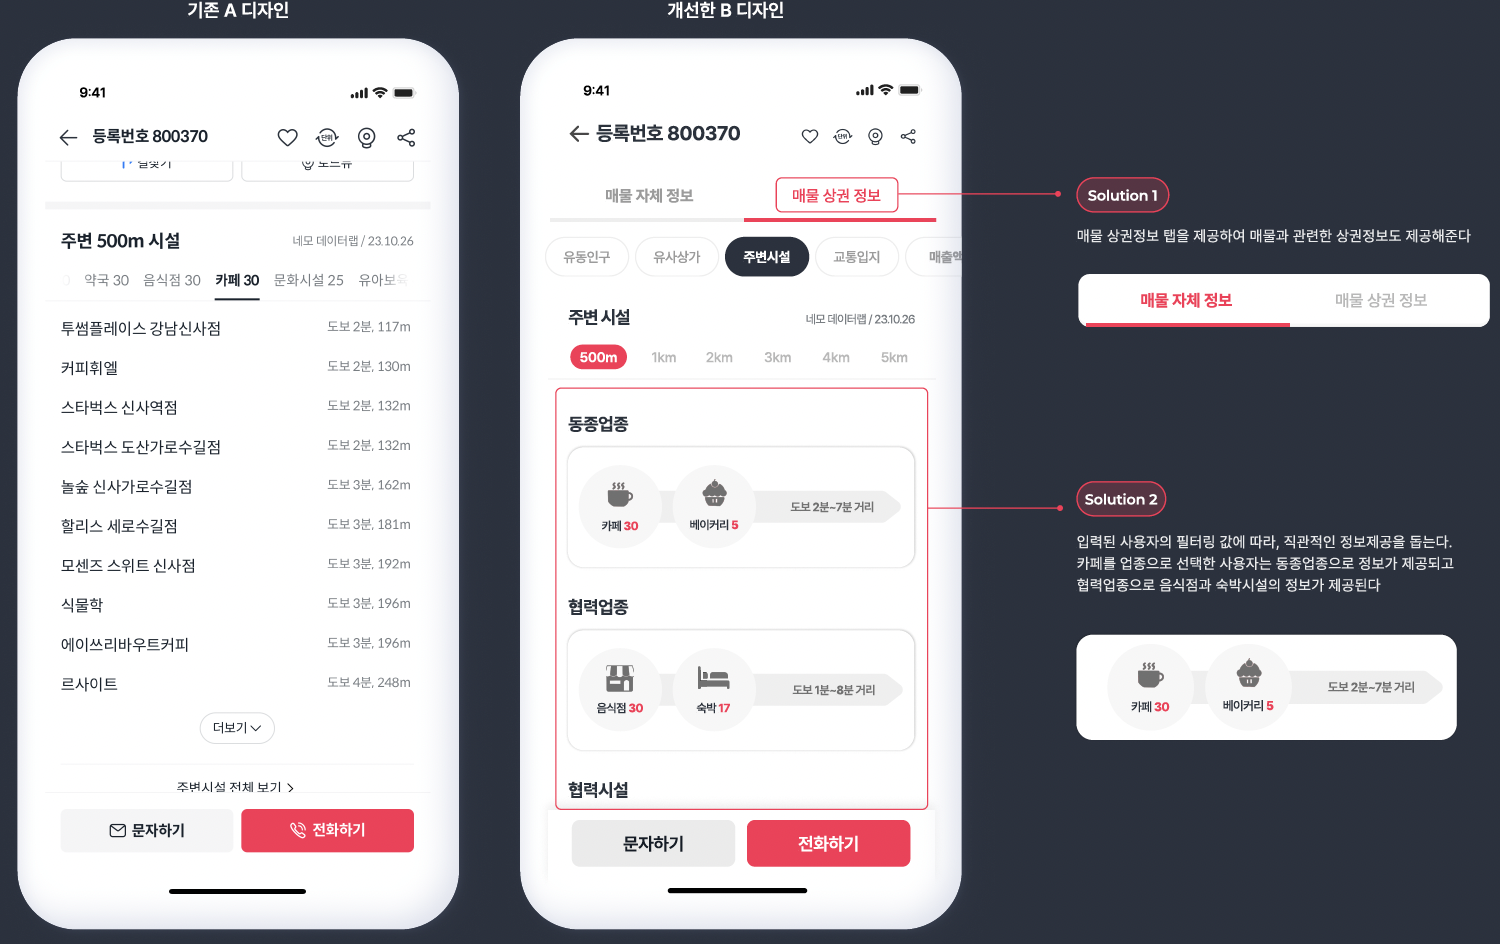
\includegraphics{img/fig25.png}

}

\caption{부동산 상권 분석 앱의 주변 상권 정보 페이지에 대한 기존
디자인(좌)과 개선 디자인(우)}

\end{figure}%

여기까지 기존 디자인의(A 디자인) 리서치와 개선 디자인(B 디자인) 제안
단원을 마치고, 다음 단계에서는 통계적 가설 검증 개념을 적용한 데이터
기반 디자인 검증(A/B테스트)에 대하여 자세히 알아보고, 개선 디자인에 대한
디자인 검증 실습을 진행하도록 하겠습니다.

(문헌 27) Aaron Gitlin, ``Becoming a data-aware designer'',
\url{https://uxdesign.cc/becoming-a-data-aware-designer-1d7614ebc3ed}

(문헌 28) Paperless Post, ``online invitations for all moments that
matter'', \url{https://www,paperlesspost.com}

\part{\textbf{part 4. 개선 디자인의 검증: A/B Testing}}

\chapter*{part 4. 개선 디자인의 검증 : A/B
Testing}\label{part-4.-uxac1cuxc120-uxb514uxc790uxc778uxc758-uxac80uxc99d-ab-testing-1}
\addcontentsline{toc}{chapter}{part 4. 개선 디자인의 검증 : A/B Testing}

\markboth{part 4. 개선 디자인의 검증 : A/B Testing}{part 4. 개선
디자인의 검증 : A/B Testing}

이번 단원에서는 전 단원에서 디자인한 개선 디자인(B 디자인)을 기존의
디자인(A 디자인)과 비교하여 KPI의 개선을 가져오는지를 통계적 방법으로
비교 검증하는 방법을 학습합니다. 먼저 A/B 테스팅을 이해하기 위한 기초
통계 개념을 공부하고, F-test, T-test의 시행과 검정 방법을 학습합니다. 각
테스트는 다양한 소프트웨어적인 시행 방법이 있으므로, 가장 많이 시행하는
방법들을 알아봅니다.

그리고 실습 프로젝트의 디자인을 설문으로 평가 검증하기 위하여 설문을
기획하고, 데이터를 수집하고, 데이터를 평가 방법에 맞추어 정리하고, A/B
테스트 값을 도출하는 실습을 합니다. 계산된 값을 해석하여 결론을
도출하고, 평가 결과를 반영하여 개선 디자인을 확정하거나 필요한 추가 개선
사항을 진행합니다. 마지막으로 이러한 디자인 과정을 지속적으로
관리해나가는 방법을 알아봅니다.

\href{ch1.\%20AB\%20테스팅을\%20위한\%20기초\%20통계와\%20가설\%20검증\%20기법.qmd}{ch1.
A/B 테스팅을 위한 기초 통계와 가설 검증 기법}

\href{ch2.\%20F-test와\%20T-test의\%20실습\%20방법들.qmd}{ch2. F-test와
T-test의 실습 방법들}

\href{ch3.\%20실습\%20과제의\%20AB\%20테스팅\%20기획.qmd}{ch3. 실습
과제의 A/B 테스팅 기획}

\href{ch4.\%20AB\%20테스팅\%20실행\%20및\%20결과의\%20해석.qmd}{ch4. A/B
테스팅 실행 및 결과의 해석}

\href{ch5.\%20AB\%20테스팅\%20결과의\%20디자인\%20반영.qmd}{ch5. A/B
테스팅 결과의 디자인 반영}

\chapter{ch1. A/B 테스팅을 위한 기초 통계와 가설 검증
기법}\label{ch1.-ab-uxd14cuxc2a4uxd305uxc744-uxc704uxd55c-uxae30uxcd08-uxd1b5uxacc4uxc640-uxac00uxc124-uxac80uxc99d-uxae30uxbc95}

실습과제 8에서 타겟 서비스의 개선안 디자인을 완료하였다면, 이제부터는
과연 새로운 개선 디자인이 기존 디자인에 비하여 KPI를 높이는 효과가
있는지를 알아보겠습니다. 우리는 이 과정을 A/B 테스팅으로 불리는 통계적
분석 기법을 사용하여 실습하려고 합니다.

A/B 테스트는 통계적으로 의미있는 데이터를 활용해서 사업적 중요성(KPI)을
기준으로 제품에 관련된 더 나은 의사결정을 하려는 목적의 평가 기법입니다.
A/B 테스트의 시행 방법은 디자인의 구현 과정에서 화면이나 기능을 여러
버전으로 만들어서 서로 다른 사용자 그룹에 각기 다른 것을 보여주고 어떤
버전이 최선의 지표를 이끌어 내는지 찾아냅니다.(20)

우선 실습에 필요한 기초적인 통계 개념들을 학습해 보겠습니다.

\section{가설과 검정}\label{uxac00uxc124uxacfc-uxac80uxc815}

가설(Hypothesis)은 앞서 설명한 바와 같이 특정 현상이나 문제에 대해 검증
가능한 예측이나 추정을 의미합니다. 그리고 검정(statistical test)이란
통계학에서 특정 가설을 검증하기 위한 과정을 의미합니다.

통계학의 가설은 귀무가설(H0)과 대립가설(H1)로 설정할 수 있는데,
귀무가설(H0)은 보통 ``차이가 없다'' 또는 ``효과가 없다''는 가설이고,
대립가설(H1)은 ``차이가 있다'' 또는 ``효과가 있다''는 가설입니다. 우리
실험에서 기존 디자인(A 디자인)의 KPI와 개선 디자인(B 디자인)의 KPI 값이
차이가 없다는 결과가 나오면 귀무가설이 채택된 것입니다.

검정 결과는 데이터에서 검정 통계량을 계산하고, 검정 통계량과 유의 수준을
비교하여 귀무가설을 기각할지 여부를 결정합니다. 유의수준 (α)은 통계적
검정에서 귀무가설을 기각할 기준이 되는 값입니다. 일반적으로 0.05(5\%)로
설정됩니다. p-value는 실제 데이터가 귀무가설 하에서 관측될 확률을 나타낸
값으로 , p-value가 유의수준(α)보다 작으면 귀무가설을 기각합니다. 즉
p-value가 유의 수준 값인 0.05보다 작으면 비교한 데이터는 `차이가 있다',
또는 '귀무가설을 기각한다'라고 판단합니다.

\section{정규성과
등분산성}\label{uxc815uxaddcuxc131uxacfc-uxb4f1uxbd84uxc0b0uxc131}

우리가 시행하려는 A/B 테스트의 방법을 통계학에서는 독립 표본 T-test라고
합니다. 이 테스트 기법을 사용하려면 우선 실험 데이터가 정규성과
등분산성을 만족해야합니다.

\begin{itemize}
\item
  정규성(Normality)이란 데이터가 정규 분포(가우시안 분포)를 따르는지를
  의미합니다. 정규 분포는 데이터가 평균을 중심으로 대칭적으로 퍼지는 종
  모양의 분포입니다. 30개 이상의 데이터가 있으면 중심극한정리(Central
  Limit Theorem)에 따라 데이터의 평균이 정규 분포에 가까워질 수 있다는
  이론이 있습니다. 그러나, 이는 데이터의 분포가 정규 분포를 따른다는
  보장은 아닙니다. 정규성을 확인하기 위해서는 여전히 통계적 검정이나
  시각적 방법을 사용하는 것이 좋습니다. 정규성을 확인하는 시각적 방법은
  히스토그램이나 Q-Q플롯으로 데이터 분포 그래프를 보고 시각적으로 정규
  분포의 형태를 갖는지 평가할 수 있습니다. 그리고 통계적 검정 방법은
  샤피로-윌크 검정(Shapiro-Wilk Test), 앤더슨-달링 검정,
  콜모고로프-스미르노프 검정 방법이 있습니다.

  우리 프로젝트에서는 실험 데이터의 수를 30개 이상으로 하여 일단
  정규성을 확보하고, 정규성 문제가 발생할 시 통계적 검정(샤피로-윌크
  검정) 방법으로 결과를 보정합니다.
\item
  등분산성(Homoscedasticity)은 두 개 이상의 그룹이 동일한 분산을
  갖는다는 것을 의미합니다. 이는 각 그룹의 데이터 분포가 동일한 정도의
  변동성을 가진다는 것을 전제로 합니다. 예를 들어, 두 반의 학생 성적을
  비교할 때, 두 반의 성적 분포가 비슷하게 퍼져 있는지 확인하는 것입니다.
  등분산성은 박스플롯(Boxplot)을 사용하여 각 그룹의 분포를 시각적으로
  비교할 수 있고, 통계적 검정 방법은 F-검정(F-test), 레빈 검정(Levene's
  Test), 바틀렛 검정(Bartlett's Test)이 있습니다. 등분산성이 충족되지
  않으면, 비모수 검정이나 등분산성을 가정하지 않는 검정을 사용합니다.

  우리 과제에서는 등분산성을 확인하기 위하여 가장 일반적으로 사용하는
  F-검정을 실습할 것입니다.
\end{itemize}

\section{F-test(F-검정)}\label{f-testf-uxac80uxc815}

F-검정은 두 그룹의 분산이 같은지 확인하는 데 유용한 통계적 방법입니다.
이를 통해 두 집단의 분산을 비교하여 등분산성을 검정할 수 있습니다.
F-검정의 방법은 F 통계량과 유의 수준을 비교하여 귀무가설(등분산성
가정)을 기각할지 여부를 결정합니다. 등분산성을 만족하지 않는 경우는
비모수 검정이나 Welch의 t-검정 같은 대체 방법을 사용하여 그룹들의 차이를
비교할 수 있습니다.

우리 실습에서는 비교 대상인 A, B 디자인의 응답 데이터에 대하여 먼저
F-test를 시행하여 등분산성을 확인하고, 등분산성을 만족하지 않으면,
등분산을 만족하지 않는 옵션으로 T-test를 실시할 예정입니다. 그럼 F-test
의 시행 방법을 아래의 건강 관리 앱 사례로 알아보겠습니다.

XXX 앱은 사용자의 일일 걸음 수, 수면 시간, 물 섭취량 등을 추적하는
헬스케어 앱이다. 최근 AI 기반의 맞춤형 건강 관리 기능을 새로 도입했다.
이 새로운 기능이 사용자의 건강 습관과 앱 사용 패턴에 미치는 영향을
테스트하고자 한다.

여기에서 기존의 디자인 (A 디자인)과 AI 맞춤형 건강 관리 기능을 적용한
개선 디자인(B 디자인)을 사용한 사람들의 물 섭취 패턴에 변화가 있는지를
알아볼 것입니다. 먼저 두 그룹(기존 디자인 사용 그룹과 개선 디자인 사용
그룹)의 물 섭취량 데이터가 등분산을 만족하는지 보겠습니다. 이하의
예제에서 통계량 측정을 위한 프로그래밍 코드는 R을 기준으로 설명하고,
실습 과제에서는 R 이외의 다른 측정 방법들도 소개하도록 하겠습니다.

\begin{Shaded}
\begin{Highlighting}[]
\CommentTok{\# 데이터 생성}
\NormalTok{before }\OtherTok{\textless{}{-}} \FunctionTok{c}\NormalTok{(}\FloatTok{1.2}\NormalTok{, }\FloatTok{1.5}\NormalTok{, }\FloatTok{1.3}\NormalTok{, }\FloatTok{1.4}\NormalTok{, }\FloatTok{1.6}\NormalTok{, }\FloatTok{1.3}\NormalTok{, }\FloatTok{1.7}\NormalTok{, }\FloatTok{1.5}\NormalTok{, }\FloatTok{1.4}\NormalTok{, }\FloatTok{1.6}\NormalTok{)  }\CommentTok{\# 섭취량, 리터 단위}
\NormalTok{after }\OtherTok{\textless{}{-}} \FunctionTok{c}\NormalTok{(}\FloatTok{1.5}\NormalTok{, }\FloatTok{1.8}\NormalTok{, }\FloatTok{1.6}\NormalTok{, }\FloatTok{1.7}\NormalTok{, }\FloatTok{2.0}\NormalTok{, }\FloatTok{1.6}\NormalTok{, }\FloatTok{2.1}\NormalTok{, }\FloatTok{1.9}\NormalTok{, }\FloatTok{1.8}\NormalTok{, }\FloatTok{1.9}\NormalTok{)}

\CommentTok{\# F{-}검정 수행}
\FunctionTok{var.test}\NormalTok{(before, after)}
\end{Highlighting}
\end{Shaded}

\begin{Shaded}
\begin{Highlighting}[]
\NormalTok{수행 결과}\SpecialCharTok{:}
\NormalTok{F test to compare two variances}

\NormalTok{data}\SpecialCharTok{:}\NormalTok{  before and after}
\NormalTok{F }\OtherTok{=} \FloatTok{0.68389}\NormalTok{, num df }\OtherTok{=} \DecValTok{9}\NormalTok{, denom df }\OtherTok{=} \DecValTok{9}\NormalTok{, p}\SpecialCharTok{{-}}\NormalTok{value }\OtherTok{=} \FloatTok{0.5804}
\NormalTok{alternative hypothesis}\SpecialCharTok{:}\NormalTok{ true ratio of variances is not equal to }\DecValTok{1}
\DecValTok{95}\NormalTok{ percent confidence interval}\SpecialCharTok{:}
 \FloatTok{0.1698687} \FloatTok{2.7533395}
\NormalTok{sample estimates}\SpecialCharTok{:}
\NormalTok{ratio of variances }
         \FloatTok{0.6838906} 
\end{Highlighting}
\end{Shaded}

위의 결과값을 해석해 보겠습니다. 결과값에서 p-value가 0.5804로 나왔네요.
p-value가 유의 수준인 0.05보다 큰 값이므로 before 데이터와 after
데이터는 분산의 차이가 없다는 귀무 가설을 채택합니다. 즉 등분산입니다.

그리고 F-검정은 3개이상 집단의 평균을 비교하여 차이 여부 검정하는
경우에도 사용합니다. 즉 비교 디자인이 세 개 이상(디자인 A, B, C안 등)
존재하는 경우는 F-검정으로 평균의 차이가 있는지를 확인할 수 있습니다.
또한 데이터가 수치 데이터가 아닌 범주 데이터일 때는 카이제곱 검정을
사용합니다.

\section{T-test (T 검정)}\label{t-test-t-uxac80uxc815}

이제 A/B 테스트의 판단 기준인 T-test에 대하여 알아보겠습니다. T-검정은
두 집단간 평균의 차이가 있는지의 여부를 검정하는 방법입니다. 두 비교
그룹의 평균값이 차이가 있으면, 두 그룹의 값은 차이가 있다고 판단하는
것입니다. T-검정에는 데이터 비교 유형에 따라 단일 표본, 독립 표본, 대응
표본의 T-검정으로 나뉘며, 각 유형에 따라 테스트의 방법(코드)이 조금
다릅니다. 위에서 본 헬스케어 앱을 가지고 각 검증 유형의 특징과 코드 수행
사례를 살펴보겠습니다.

\begin{itemize}
\item
  \textbf{단일 표본 T-test} : 측정한 데이터의 평균이 특정 기준보다
  유의미하게 다른지 혹은 큰지/작은지를 알아보는 분석 방법입니다. 아래와
  같은 R코드를 사용합니다.

  R 문법: t.test(관측치, alternative = 판별 방향, mu=특정기준,
  conf.level = 신뢰수준)

  alternative에는 ``greater'', ``less'', ``two.sided''가 있습니다. 각각
  큰지/작은지/같은지를 구분하라는 명령입니다.

  신뢰수준 (Confidence Level)은 추정값이 참 값 범위 내에 있을 확률
  의미하며, 예를들어 95\% 신뢰수준은 추정값이 95\%의 확률로 참 값 범위
  내에 있다는 의미입니다. 신뢰수준과 유의수준은 `1-신뢰수준=유의수준' 의
  수식이 성립합니다. 아래의 가설로 T-검정을 해봅시다.

  가설: AI 맞춤 관리 기능 도입 후 사용자들의 일일 평균 걸음 수가
  8000보를 넘었다.

  R 코드로 T-검정을 실행합니다. 예시에 사용한 csv 형식의 데이터는
  100명의 A디자인 사용 그룹, 100명의 B디자인 사용 그룹의 건강 정보를
  가정하여 인공지능이 생성한 데이터입니다. 예시 데이터의 열 정보는
  다음과 같습니다. T-test 옵션은 A 디자인 사용자의 데이터 평균 보다 B
  디자인 사용자의 평균이 큰지를 검정하는 ``greater''옵션을 사용했습니다.

  \begin{itemize}
  \tightlist
  \item
    daily\_steps: 일일 걸음 수
  \item
    sleep\_hours: 수면 시간 (시간)
  \item
    exercise\_minutes: 운동 시간 (분)
  \item
    stress\_level: 스트레스 수준
  \item
    water\_intake\_pre: AI 맞춤 관리 기능 도입 이전 물 섭취량
  \item
    water\_intake\_post: AI 맞춤 관리 기능 도입 이후 물 섭취량
  \end{itemize}

\begin{Shaded}
\begin{Highlighting}[]
\CommentTok{\# 필요한 라이브러리를 로드합니다.}
\FunctionTok{library}\NormalTok{(dplyr)}
\FunctionTok{library}\NormalTok{(ggplot2)}

\CommentTok{\# CSV 파일을 로드합니다.}
\NormalTok{df }\OtherTok{\textless{}{-}} \FunctionTok{read.csv}\NormalTok{(}\StringTok{"mupdated\_health\_data.csv"}\NormalTok{)}

\CommentTok{\# 단일 표본 t{-}검정을 수행합니다.}
\NormalTok{t\_test\_result }\OtherTok{\textless{}{-}} \FunctionTok{t.test}\NormalTok{(df}\SpecialCharTok{$}\NormalTok{daily\_steps, }\AttributeTok{mu =} \DecValTok{8000}\NormalTok{, }\AttributeTok{alternative =} \StringTok{"greater"}\NormalTok{)}

\CommentTok{\# 결과를 출력합니다.}
\FunctionTok{print}\NormalTok{(t\_test\_result)}
\end{Highlighting}
\end{Shaded}

\begin{Shaded}
\begin{Highlighting}[]
\NormalTok{One Sample t}\SpecialCharTok{{-}}\NormalTok{test}

\NormalTok{data}\SpecialCharTok{:}\NormalTok{  df}\SpecialCharTok{$}\NormalTok{daily\_steps}
\NormalTok{t }\OtherTok{=} \FloatTok{0.21082}\NormalTok{, df }\OtherTok{=} \DecValTok{199}\NormalTok{, p}\SpecialCharTok{{-}}\NormalTok{value }\OtherTok{=} \FloatTok{0.4166}
\NormalTok{alternative hypothesis}\SpecialCharTok{:}\NormalTok{ true mean is greater than }\DecValTok{8000}
\DecValTok{95}\NormalTok{ percent confidence interval}\SpecialCharTok{:}
 \FloatTok{7880.736}      \ConstantTok{Inf}
\NormalTok{sample estimates}\SpecialCharTok{:}
\NormalTok{mean of x }
 \FloatTok{8017.439} 
\end{Highlighting}
\end{Shaded}

  이 데이터의 경우 95\% 신뢰 수준에서 p-value가 0.4166이므로 유의 수준
  0.05보다 큽니다. 그러므로 개선된 앱이 사용자들의 걸음 수를 개선하지는
  못했습니다. T-검정 결과를 그래프로 표현하면 아래와 같습니다. 기준 값인
  8,000보를 중심으로 수집된 걸음수 값의 분포를 히스토그램으로 보여주고
  있습니다.

\begin{Shaded}
\begin{Highlighting}[]
\CommentTok{\# 일일 걸음 수 분포를 시각화합니다.}
\FunctionTok{ggplot}\NormalTok{(df, }\FunctionTok{aes}\NormalTok{(}\AttributeTok{x =}\NormalTok{ daily\_steps)) }\SpecialCharTok{+}
  \FunctionTok{geom\_histogram}\NormalTok{(}\AttributeTok{binwidth =} \DecValTok{500}\NormalTok{, }\AttributeTok{fill =} \StringTok{"blue"}\NormalTok{, }\AttributeTok{alpha =} \FloatTok{0.7}\NormalTok{) }\SpecialCharTok{+}
  \FunctionTok{geom\_vline}\NormalTok{(}\FunctionTok{aes}\NormalTok{(}\AttributeTok{xintercept =} \FunctionTok{mean}\NormalTok{(daily\_steps)), }\AttributeTok{color =} \StringTok{"red"}\NormalTok{, }\AttributeTok{linetype =} \StringTok{"dashed"}\NormalTok{, }\AttributeTok{size =} \DecValTok{1}\NormalTok{) }\SpecialCharTok{+}
  \FunctionTok{labs}\NormalTok{(}\AttributeTok{title =} \StringTok{"Distribution of Daily Steps"}\NormalTok{,}
   \AttributeTok{x =} \StringTok{"Daily Steps"}\NormalTok{,}
   \AttributeTok{y =} \StringTok{"Frequency"}\NormalTok{,}
   \AttributeTok{subtitle =} \FunctionTok{sprintf}\NormalTok{(}\StringTok{"T{-}test p{-}value: \%s"}\NormalTok{, formatted\_p\_value)) }\SpecialCharTok{+}
  \FunctionTok{theme\_minimal}\NormalTok{()}
\end{Highlighting}
\end{Shaded}
\end{itemize}

\begin{figure}[H]

{\centering 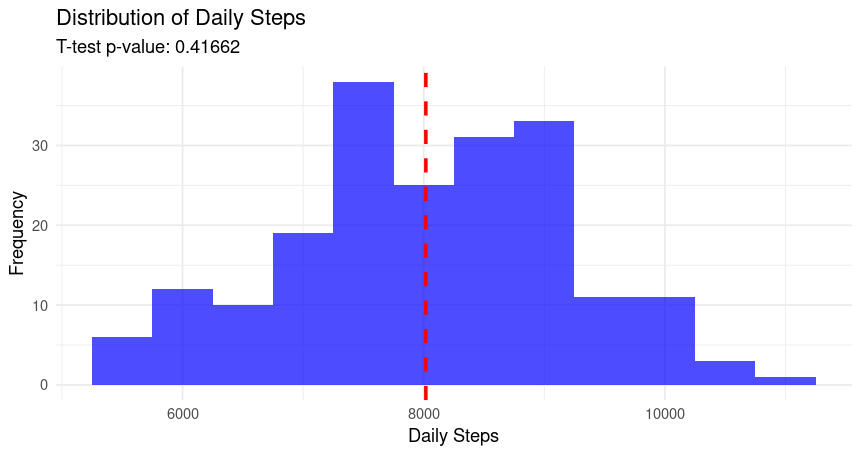
\includegraphics{img/fig26.png}

}

\caption{데이터에 대한 단일 표본 T-test 결과의 시각화 그래프}

\end{figure}%

\begin{itemize}
\item
  \textbf{독립 표본 T-test:} 서로 다른 두개의 그룹 간 평균의 차이가
  유의미 한지 여부를 판단하기 위한 검정입니다. 두개의 표본이 ``독립''적
  이기 위해서는 두개의 표본이 서로 관계 없는 모집단에서 추출 되었고,
  표본 간에는 아무런 관계가 없어야 합니다. 우리가 사용하는 A/B 테스트
  기법은 독립 표본 T-test로 기존 디자인(A 디자인)의 사용자와 개선
  디자인(B 디자인)의 사용자는 서로 다른 사용자 집단이고, 관련이 없어야
  합니다. 그래서 A 디자인의 사용자와 B 디자인의 사용자를 따로 모집하여
  테스트를 시행합니다.

  R에서 독립표본 t-test를 하는 방법은 두가지가 있습니다. 하나는 분석을
  원하는 두 집단의 평균을 각각 별개의 벡터 객체로 만들어 입력하는 방법
  입니다. 유형 1 문법은 t.test(group 1의 관측치, group2의 관측치, t-test
  유형, 신뢰범위)와 같고, 유형2의 문법은 하나의 데이터 프레임에서 집단을
  구분하고자 하는 기준을 입력하는 것으로,
  t.test(관측치\textasciitilde 집단 구분 기준, 데이터프레임, t-test
  유형, 신뢰범위)와 같이 수행합니다.

  가설: AI 맞춤 관리를 받은 그룹이 그렇지 않은 그룹보다 주간 운동 시간이
  더 길다.

\begin{Shaded}
\begin{Highlighting}[]
\CommentTok{\# Calculate weekly exercise minutes}
\NormalTok{df }\OtherTok{\textless{}{-}}\NormalTok{ df }\SpecialCharTok{\%\textgreater{}\%} \FunctionTok{mutate}\NormalTok{(}\AttributeTok{weekly\_exercise\_minutes =}\NormalTok{ exercise\_minutes }\SpecialCharTok{*} \DecValTok{7}\NormalTok{)}

\CommentTok{\# Perform independent two{-}sample t{-}test}
\NormalTok{t\_test\_result }\OtherTok{\textless{}{-}} \FunctionTok{t.test}\NormalTok{(weekly\_exercise\_minutes }\SpecialCharTok{\textasciitilde{}}\NormalTok{ group, }\AttributeTok{data =}\NormalTok{ df, }\AttributeTok{alternative =} \StringTok{"greater"}\NormalTok{)}

\CommentTok{\# Print the result}
\FunctionTok{cat}\NormalTok{(}\FunctionTok{sprintf}\NormalTok{(}\StringTok{"data: weekly\_exercise\_minutes by group}\SpecialCharTok{\textbackslash{}n}\StringTok{t = \%.4f, df = \%.2f, p{-}value = \%.15f}\SpecialCharTok{\textbackslash{}n}\StringTok{alternative hypothesis: true difference in means between group A and group B is greater than 0}\SpecialCharTok{\textbackslash{}n}\StringTok{95 percent confidence interval:}\SpecialCharTok{\textbackslash{}n}\StringTok{ 156.8696      Inf}\SpecialCharTok{\textbackslash{}n}\StringTok{sample estimates:}\SpecialCharTok{\textbackslash{}n}\StringTok{mean in group A = \%.3f, mean in group B = \%.3f}\SpecialCharTok{\textbackslash{}n}\StringTok{"}\NormalTok{, }
\NormalTok{            t\_test\_result}\SpecialCharTok{$}\NormalTok{statistic, t\_test\_result}\SpecialCharTok{$}\NormalTok{parameter, t\_test\_result}\SpecialCharTok{$}\NormalTok{p.value, }
\NormalTok{            t\_test\_result}\SpecialCharTok{$}\NormalTok{estimate[}\DecValTok{1}\NormalTok{], t\_test\_result}\SpecialCharTok{$}\NormalTok{estimate[}\DecValTok{2}\NormalTok{]))}
\end{Highlighting}
\end{Shaded}

\begin{Shaded}
\begin{Highlighting}[]
\NormalTok{data}\SpecialCharTok{:}\NormalTok{ weekly\_exercise\_minutes by group}
\NormalTok{t }\OtherTok{=} \FloatTok{7.1528}\NormalTok{, df }\OtherTok{=} \FloatTok{192.59}\NormalTok{, p}\SpecialCharTok{{-}}\NormalTok{value }\OtherTok{=} \FloatTok{0.000000000008641}
\NormalTok{alternative hypothesis}\SpecialCharTok{:}\NormalTok{ true difference }\ControlFlowTok{in}\NormalTok{ means between group A and group B is greater than }\DecValTok{0}
\DecValTok{95}\NormalTok{ percent confidence interval}\SpecialCharTok{:}
 \FloatTok{156.8696}      \ConstantTok{Inf}
\NormalTok{sample estimates}\SpecialCharTok{:}
\NormalTok{mean }\ControlFlowTok{in}\NormalTok{ group A }\OtherTok{=} \FloatTok{1056.917}\NormalTok{, mean }\ControlFlowTok{in}\NormalTok{ group B }\OtherTok{=} \FloatTok{852.906}
\end{Highlighting}
\end{Shaded}

  T-test 결과를 해석하면, p-value가 매우 작게 나왔죠. 95\% 신뢰 수준에서
  두 값의 차이가 있다는 뜻이므로 AI 맞춤 관리 기능이 사용자들의 주간
  운동 시간을 더 길게 한다는 판단을 할 수 있습니다. 아래의 박스 플롯
  그래프를 보면 두 집단의 값 분포가 차이가 나는 것을 시각적으로도 확인할
  수 있습니다.

  \begin{figure}[H]

  {\centering 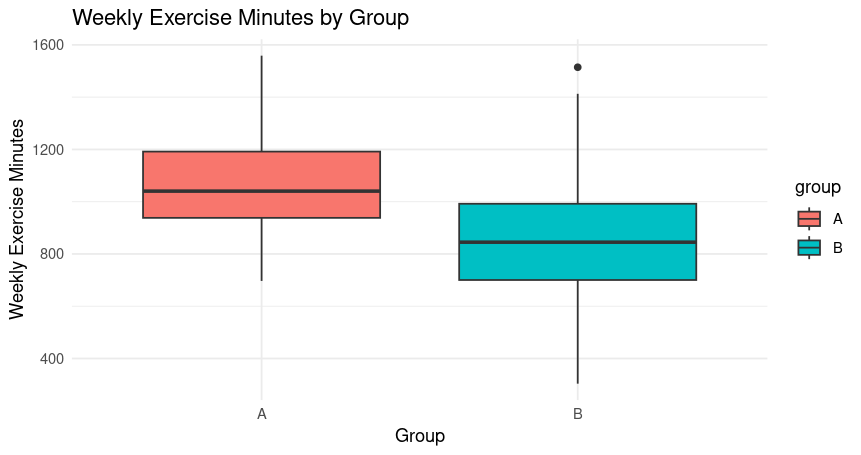
\includegraphics{img/fig27.png}

  }

  \caption{데이터의 박스 플롯 그래프}

  \end{figure}%
\item
  \textbf{대응 표본 T-test:} 대응표본 t-test는 동일한 집단의 전-후
  차이를 비교하기 위해 사용됩니다.

  예를 들어 초콜렛을 하루 30g씩 섭취하는 것이 수면 시간에 영향을
  미치는지 여부나, 과외를 받는 것이 학교 성적에 영향을 미치는지 등등
  특정 변인의 영향을 측정하기 위해 주로 사용됩니다. 주의할 점은 대응
  표본은 실험 전-후를 비교하는 것이기 때문에 입력하는 관측치의 수가
  반드시 같고, 동일 집단 이어야 합니다.

  가설: AI 맞춤 관리 기능 도입 후 사용자들의 일일 평균 물 섭취량이
  증가했다.

  이번에는 F-test 에서 사용한 예제를 이어서 T-test에서도 사용하겠습니다.

\begin{Shaded}
\begin{Highlighting}[]
\CommentTok{\# 데이터 생성}
\NormalTok{before }\OtherTok{\textless{}{-}} \FunctionTok{c}\NormalTok{(}\FloatTok{1.2}\NormalTok{, }\FloatTok{1.5}\NormalTok{, }\FloatTok{1.3}\NormalTok{, }\FloatTok{1.4}\NormalTok{, }\FloatTok{1.6}\NormalTok{, }\FloatTok{1.3}\NormalTok{, }\FloatTok{1.7}\NormalTok{, }\FloatTok{1.5}\NormalTok{, }\FloatTok{1.4}\NormalTok{, }\FloatTok{1.6}\NormalTok{)  }\CommentTok{\# 리터 단위}
\NormalTok{after }\OtherTok{\textless{}{-}} \FunctionTok{c}\NormalTok{(}\FloatTok{1.5}\NormalTok{, }\FloatTok{1.8}\NormalTok{, }\FloatTok{1.6}\NormalTok{, }\FloatTok{1.7}\NormalTok{, }\FloatTok{2.0}\NormalTok{, }\FloatTok{1.6}\NormalTok{, }\FloatTok{2.1}\NormalTok{, }\FloatTok{1.9}\NormalTok{, }\FloatTok{1.8}\NormalTok{, }\FloatTok{1.9}\NormalTok{)}

\CommentTok{\# T{-}검정 수행}
\FunctionTok{t.test}\NormalTok{(before,after, }\AttributeTok{paired=}\ConstantTok{TRUE}\NormalTok{, }\AttributeTok{conf.level =} \FloatTok{0.95}\NormalTok{)}
\end{Highlighting}
\end{Shaded}

\begin{Shaded}
\begin{Highlighting}[]
\NormalTok{Paired t}\SpecialCharTok{{-}}\NormalTok{test}

\NormalTok{data}\SpecialCharTok{:}\NormalTok{  before and after}
\NormalTok{t }\OtherTok{=} \SpecialCharTok{{-}}\FloatTok{20.821}\NormalTok{, df }\OtherTok{=} \DecValTok{9}\NormalTok{, p}\SpecialCharTok{{-}}\NormalTok{value }\OtherTok{=} \FloatTok{6.367e{-}09}
\NormalTok{alternative hypothesis}\SpecialCharTok{:}\NormalTok{ true mean difference is not equal to }\DecValTok{0}
\DecValTok{95}\NormalTok{ percent confidence interval}\SpecialCharTok{:}
 \SpecialCharTok{{-}}\FloatTok{0.3769409} \SpecialCharTok{{-}}\FloatTok{0.3030591}
\NormalTok{sample estimates}\SpecialCharTok{:}
\NormalTok{mean difference }
          \SpecialCharTok{{-}}\FloatTok{0.34} 
\end{Highlighting}
\end{Shaded}

  결과를 해석해 보겠습니다. p-value가 6.367e-09이 나왔네요. 이것은
  66.367곱하기 (0.1)의 9제곱이라는 뜻으로 매우 작은 수입니다. 즉 95\%
  신뢰 수준에서 두 값의 차이가 있다고 판단합니다. 새로운 기능은
  사용자들의 물 섭취량을 개선했습니다.

  이상으로 T-test의 유형별 데이터 특성과 시행 방법을 알아보았습니다.
  학습한 검정 기법들을 데이터의 특성에 맞게 적용하여 실습해보기
  바랍니다.
\end{itemize}

(문헌 20) 로라 클라인, (김수영, 박기석 역), 『린 스타트업 실전 UX』,
한빛미디어,(2014)

\chapter{ch2. F-test와 T-test의 실습
방법들}\label{ch2.-f-testuxc640-t-testuxc758-uxc2e4uxc2b5-uxbc29uxbc95uxb4e4}

앞 장에서는 가설 검정의 개념과 R 코드를 사용한 예제들을 학습했지만,
F-테스트나 T-테스트의 수행 방법은 다양합니다. 오피스 문서 도구인 구글
스프레드 시트나 엑셀 함수를 사용하여 매우 간단하게 결과를 얻을 수 있고,
통계계산기, 또는 AI 서비스를 통해서도 값을 얻고, 결과 해석에 대한 도움도
받을 수 있습니다. 앞으로 업무 환경에 맞게 다른 방법들을 사용할 수 있으니
여러가지 검정 방법들을 살펴보겠습니다.

\section{구글 스프레드 시트를 사용한 가설 검정 (F-test,
T-test)}\label{uxad6cuxae00-uxc2a4uxd504uxb808uxb4dc-uxc2dcuxd2b8uxb97c-uxc0acuxc6a9uxd55c-uxac00uxc124-uxac80uxc815-f-test-t-test}

아래의 링크를 보면 구글 스프레드 시트와 엑셀에서 사용할 수 있는 FTEST,
TTEST 함수에 관한 설명이 나와있습니다. 앞 장에서 함수 이해에 필요한
개념들을 학습했으므로 설명이 잘 이해될 것입니다. 함수의 사용 방법은
설명에 나와 있듯이 아주 쉽습니다. 답을 넣고 싶은 셀에서 상단 리본 메뉴의
함수\textgreater 통계\textgreater FTEST/ TTEST를 선택하고, 적용할 데이터
범위와 옵션을 지정해 주면 검정에 필요한 p-value 값을 바로 출력해줍니다.
데이터량이 많고, 데이터 편집이 필요할 때는 R과 같이 프로그래밍적인
방법이 좋지만, 데이터량이 적은 경우에는 오피스 도구로 충분히 원하는 검정
결과를 얻을 수 있습니다. (29)(30)

\href{https://support.google.com/docs/answer/7004183?hl=ko&ref_topic=3105600}{FTEST}

\href{https://support.google.com/docs/answer/6055837?hl=ko}{TTEST}

\section{엑셀의 분석도구팩을 사용한 가설 검정 (F-test,
T-test)}\label{uxc5d1uxc140uxc758-uxbd84uxc11duxb3c4uxad6cuxd329uxc744-uxc0acuxc6a9uxd55c-uxac00uxc124-uxac80uxc815-f-test-t-test}

이번에는 엑셀에서 제공하는 분석도구팩을 사용하여 좀 더 풍부한 해설 값을
출력해보겠습니다. 우선 엑셀 분석도구팩을 설치해야합니다. 사용 컴퓨터가
윈도우 PC인 경우 엑셀 상단 리본메뉴의 파일 \textgreater 옵션
\textgreater 추가기능 \textgreater 이동 \textgreater{} 분석도구팩을
선택하여 설치합니다. 사용 컴퓨터가 맥 PC인 경우 엑셀 리본메뉴의 데이터
\textgreater 분석도구 \textgreater 분석도구팩을 선택하여 설치합니다.

분석 도구팩 설치 후, 상단 리본메뉴 데이터\textgreater 데이터
분석\textgreater{} T검정/ F 검정 옵션선택 \textgreater{} 범위 설정
\textgreater{} 기타 출력 옵션 설정을 하면 아래 그림의 하단 표와 같이
정리된 표 형태로 검정 테스트 관련 값들이 출력됩니다.

{[}그림 28{]}은 수업에서 사용한 연습 데이터로 3개 설문 문항에 대하여 각
문항의 A디자인(우), B디자인(좌)에 대한 사용자 응답 결과를 대응하여
입력하였고, 각 문항 별로 등분산 여부(FTEST)와 두 값의 차이 여부(TTEST)를
24, 25행에 출력한 사례입니다. 그리고 그림에서 상단 입력 내용 창에는 문항
2에 대하여 엑셀 함수 메뉴를 사용한 E25셀의 TTEST엑셀 함수 옵션을
보여줍니다. 그리고 28행 부터는 엑셀의 분석도구팩을 사용하여 TTEST 분석
내용을 표로 출력하였습니다.

결과 내용을 보면 3개 문항 모두 FTEST에서 p-value가 0.05보다 크므로 두
그룹의 분산 차이가 없다는 등분산 만족 결과를 보여주고, 있고, TTEST에서
문항 1, 2는 p-value가 0.05보다 커서 두 그룹의 차이가 없다. 즉 결과가
개선되지 않았음을 알 수 있고, 문항 5는 p-value가 0.05보다 작아서 두 값의
차이가 있다. 즉, 디자인 B의 응답 값이 더 높다, 개선되었다는 판단을 할 수
있습니다. 1번 문항의 경우 31행의 평균값(Mean)을 보면 A디자인의 값이 더
높습니다. 하지만 T검정 값은 통계적으로 판단할 때 두 값이 차이가 없다고
판단합니다. 문항 2의 경우 B디자인의 평균값이 조금 더 높지만 이것은 T검정
값으로 볼 때 통계적 의미가 없는 차이여서 두 값의 차이가 없다고
판단했습니다. 이렇게 각 그룹의 평균값이 차이가 난다는 것만으로는 어떤
그룹의 값이 더 높거나 낮다고 판단할 수는 없다는 것을 알 수 있습니다.

\begin{figure}[H]

{\centering 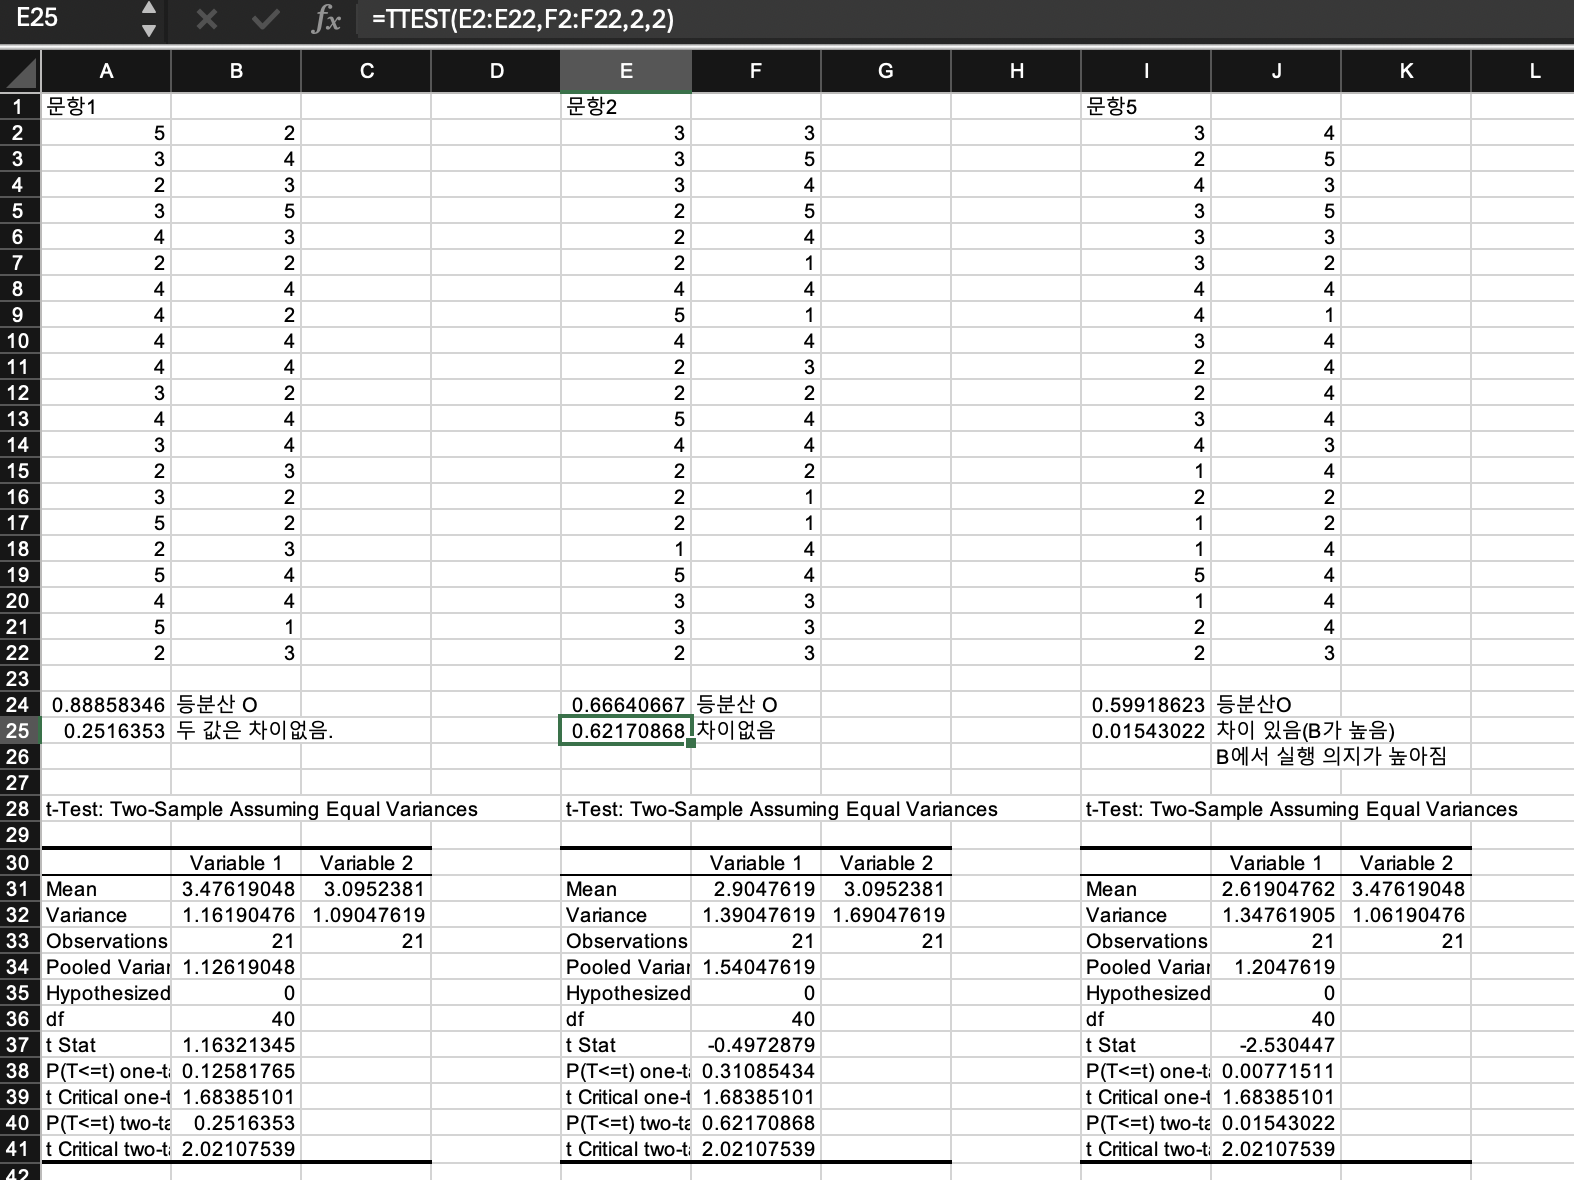
\includegraphics{img/fig28.png}

}

\caption{샘플 데이터에 대한 엑셀의 FTEST, TTEST 결과 출력 화면}

\end{figure}%

여기까지 수업을 하고나면, 어려워 보이던 F검정, T검정의 방법이 너무
간단해서 놀라고, 당연히 KPI가 개선 될 것으로 확신했던 개선 디자인 B의
값이 A디자인과 차이가 없다는 결과가 많이 나와서 다시 한 번 놀랍니다.
통계적 검정의 결과는 매우 보수적인 편입니다. 정말 확실한 차이가 있어야
두 그룹이 차이가 있다고 판정합니다. 이에 대한 자세한 대응 방법은 다음
단원의 실습 과제에서 더 공부하도록 하겠습니다.

\section{통계 계산기: T-Test Calculator를 사용한 가설
검정}\label{uxd1b5uxacc4-uxacc4uxc0b0uxae30-t-test-calculatoruxb97c-uxc0acuxc6a9uxd55c-uxac00uxc124-uxac80uxc815}

아래 {[}그림 29{]}는 {[}그림 28{]}의 5번 문항 데이터를 T-Test Calculator
서비스에 넣어서 데이터 분석과 해석을 출력한 사례입니다. 이것은 웹기반의
통계 계산 서비스를 활용한 것으로, GUI메뉴로 데이터를 입력하면, 해당 통계
계산을 해서 출력과 자세한 데이터 분석을 제공합니다. 현재 테스트
화면에서는 두 데이터의 정규성에 문제가 있는 것으로 진단 되었습니다. 우리
테스트의 데이터 갯수가 적기 때문에 정규성 만족 문제가 발생했고, 이
문제를 해결하기 위해 다른 방법(Calculate Mann-Whitney)으로 분석해 볼
것을 권장하고 있습니다. 또한 데이터의 분석 내용을 그래프로 정리하여
이해하기 쉽게 해설해주고 있습니다.(31) 이렇게 통계 계산기 웹서비스를
사용하면 데이터 분석 인사이트에 대한 풍부한 해설과 추천 의견을 받아 문제
해결을 할 수 있습니다. 다만 해설에서 다루는 용어와 정의에 대한 이해
역량이 필요합니다. 어려운 해설 부분도 인공지능 서비스의 도움을 받으면
되니까 크게 걱정하지는 않아도 됩니다.

\href{https://www.statskingdom.com/140MeanT2eq.html}{Two Sample T-Test}

\begin{figure}[H]

{\centering 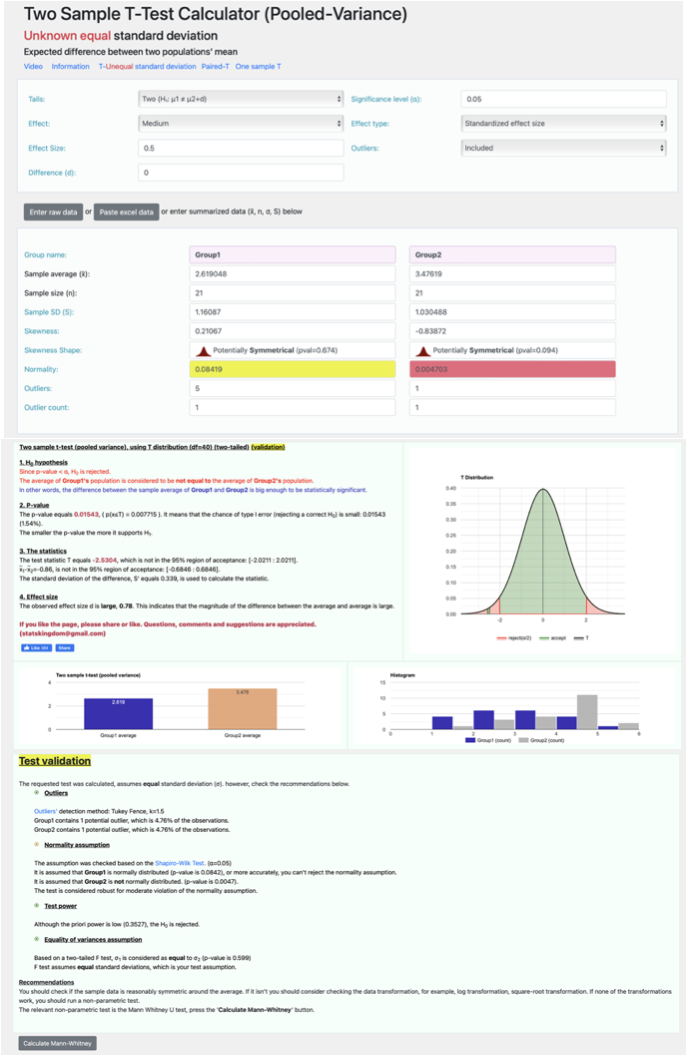
\includegraphics{img/fig29.png}

}

\caption{TTest Calculator의 실행 화면}

\end{figure}%

참고로, 정규성을 불만족한 경우 (관측값이 30개가 안되는 경우)는 T-test가
부적합하므로 아래의 정규성 검정 테스트를 해보고, 샘플이 정규분포가
아니거나 수가 적을 때, 모수에 대한 가정을 전제로 하지 않고 모집단의
형태에 관계없이 주어진 데이터에서 직접 확률을 계산하는 Mann-Whitney U
test 를 사용합니다.

\begin{itemize}
\item
  정규성 검정 (Shapiro-Wilk test)(32)
  \href{https://www.statskingdom.com/shapiro-wilk-test-calculator.html}{Shapiro-Wilk
  test calculator: normality calculator, Q-Q plot}
\item
  비모수 검정(Mann-Whitney U test)(33)
  \href{https://www.statskingdom.com/170median_mann_whitney.html}{Mann-Whitney
  U test}
\end{itemize}

\section{사용자 로그 데이터로 T-test 하기: e-commerce business A/B test
case
study}\label{uxc0acuxc6a9uxc790-uxb85cuxadf8-uxb370uxc774uxd130uxb85c-t-test-uxd558uxae30-e-commerce-business-ab-test-case-study}

데이터 과학 관련 유투버인 Emma Ding은 온라인 서비스의 A/B 테스팅 사례를
아래 제시한 영상으로 설명하였습니다. (34) 영상 내용은 온라인 쇼핑몰
운영하는 A기업이 고객 경험을 향상시키고 매출도 올리고 싶어서 여러 전략을
고민하던 중, `결제 페이지에 유사 상품 보여주는 기능' 도입하면 구매 품목
늘릴 수 있을 것 같다는 아이디어를 냈으나, 이 아이디어가 오히려 결제에
집중 못 하게 해서 구매 포기하게 만들 수도 있지 않을까 하는 걱정도 있어서
'결제 페이지에 유사 상품 보여주는 기능'의 도입 여부를 결정하고자 A/B
테스트를 진행하는 과정을 설명합니다.

\begin{itemize}
\item
  실험 목표: 유사 상품 기능이 고객 구매에 얼마나 영향 주는지, 수익 증대
  효과 있는지를 분석합니다.
\item
  KPI: 사용자당 평균 구매 금액 (ARPU:Average Revenue Per User)가 2\$
  이상 증가한다.
\item
  실험군:

  \begin{itemize}
  \tightlist
  \item
    대조군: 기존 결제 페이지 그대로 유지 (A 디자인)
  \item
    처리군 1: 결제 페이지 아래에 유사 상품 섹션 추가 (B 디자인)
  \item
    처리군 2: 결제 페이지 중앙에 유사 상품 팝업 창 띄움 (B' 디자인)
  \end{itemize}
\item
  표본:

  \begin{itemize}
  \tightlist
  \item
    결제 페이지 들어오는 모든 고객들을 각 그룹에 랜덤하게 배정해서 실험
    결과 객관적으로 나오도록 함.
  \item
    통계적으로 의미 있는 결과 얻으려면 각 그룹에 충분한 수의 사람들이
    있어야 함.
  \item
    사례는 그룹당(대조군, 처리군1, 처리군2) 1,600명씩 총 4,800명 조사,
    일 단위로 조사 인원 비율을 점차 늘려 조사함.
  \end{itemize}
\item
  실험 기간: 요일별로 차이가 있을 수 있으니까 최소 일주일 이상 진행
\item
  데이터 분석 및 결과 해석

  \begin{itemize}
  \tightlist
  \item
    처리군 1 (유사 상품 섹션, B디자인): 기존이랑 비교하여 ARPU는
    실질적인 증가가 있었지만, 통계적으로 유의미한 차이는 없었음.
  \item
    처리군 2 (유사 상품 팝업 창, B'디자인): ARPU는 실질적 증가가 있었고,
    통계적으로도 유의미하게 증가했지만, 팝업 창에 대한 고객 선호도는
    고려해야함.
  \end{itemize}
\item
  결론 및 후속 조치

  이번 A/B 테스트 결과를 바탕으로 A기업은 다음의 후속 조치를 취하기로
  함.

  \begin{itemize}
  \tightlist
  \item
    처리군 1 (유사 상품 섹션): 유사 상품 추천하는 알고리즘 개선하고
    디자인을 바꿔서 사용자 경험 좋게 만들고 다시 A/B 테스트 해보기로 함
  \item
    처리군 2 (유사 상품 팝업 창): 팝업 창 디자인을 개선해서 불편한 점을
    줄이고 구매 단가를 높이는 방법 찾아보기로 함
  \end{itemize}
\end{itemize}

이와같이 A/B 테스트는 한 번 하고 끝나는 게 아니라, 평가 결과를 바탕으로
반복적으로 개선하고 검증하면서 최적화된 결과 만들어나가는 데 활용할 수
있습니다.

\url{https://www.youtube.com/watch?v=VuKIN9S8Ivs}

(문헌 29) 구글Docs 편집기 고객센터, ``FTEST'',
\url{https://support.google.com/docs/answer/7004183?hl=ko&ref_topic=3105600}

(문헌 30) 구글Docs 편집기 고객센터, ``TTEST'',
\url{https://support.google.com/docs/answer/6055837?hl=ko}

(문헌 31) Statistics Kingdom, ``Two Sample T-Test Calculator'',
\url{https://www.statskingdom.com/140MeanT2eq.html}

(문헌 32) Statistics Kingdom, ``Shapiro-Wilk Test Calculator'',
\url{https://www.statskingdom.com/shapiro-wilk-test-calculator.html}

(문헌 33) Statistics Kingdom, ``Mann Whitney U test calculator (Wilcoxon
rank-sum)'',
\url{https://www.statskingdom.com/170median_mann_whitney.html}

(문헌 34) Emma Ding, ``A/B Testing Real-Life Example'',
\url{https://www.youtube.com/watch?v=VuKIN9S8Ivs}

\chapter{ch3. 실습 과제의 A/B 테스팅
기획}\label{ch3.-uxc2e4uxc2b5-uxacfcuxc81cuxc758-ab-uxd14cuxc2a4uxd305-uxae30uxd68d}

이제는 이번 단원에서 공부한 A/B 테스팅 방법론을 바탕으로 우리가 진행한
실습과제의 A디자인과 B디자인의 KPI가 차이가 있는지를 실험해보겠습니다.

우리 실습과제 프로젝트의 특징은 A/B 테스팅을 설문의 방법으로 한다는
것입니다. 그 이유는 우리가 실제 서비스 로그 데이터에 접근하기 어렵기
때문이라고 했었죠. 로그 데이터가 사용자의 행동을 그대로 반영하는 반면,
설문은 사용자가 의식적으로 답을 생각해내는 것이므로, 실제 행동 내용과는
다른 주관성의 개입 여지가 있습니다. 그래서 설문으로 A/B 테스팅을 하는
경우는 서비스 로그 데이터를 사용하는 방법에 비하여 아래와 같이 몇가지
고려할 점이 더 있습니다.

\section{설문을 통한 A/B 테스트를 기획할 때 유의할
점}\label{uxc124uxbb38uxc744-uxd1b5uxd55c-ab-uxd14cuxc2a4uxd2b8uxb97c-uxae30uxd68duxd560-uxb54c-uxc720uxc758uxd560-uxc810}

\begin{itemize}
\tightlist
\item
  적절한 샘플 크기와 설문 문항수: 충분한 데이터 수집을 위해 설문
  응답자가 많아야 합니다. 최소 30명 이상의 응답자가 필요합니다. 우리
  실험에서는 A 디자인에 대한 응답자 30명 이상, B디자인에 대한 응답자
  30명 이상이 필요합니다. 두 그룹의 응답자 인원이 똑같지는 않아도
  됩니다. 다만 너무 응답자 차이가 많이 나면 정규성과 분산 차이가 있을 수
  있으므로, 비슷한 수준에서 결정합니다. 문항 수는 너무 많으면 응답자
  피로가 발생하므로, 핵심 질문에 집중해 10\textasciitilde15문항 정도가
  적절합니다. 우리 실험에서는 되도록 10개 문항 이하로 합니다.
\item
  설문 질문 작성 시 고려할 점:

  \begin{itemize}
  \tightlist
  \item
    명확성: 질문이 이해하기 쉽고 명확해야 하며, 이중 부정문을 피합니다.
    설문 대상자에게 적합한 용어와 서술 방법을 사용하고, 설문 대상자는
    사용자이지, 전문가가 아니므로 디자인이나 기술 관련 기술 용어들을
    쓰는 것을 지양합니다.
  \item
    중립적 표현: 편향된 질문이나 응답을 유도하는 표현을 피합니다. 특히
    A,B 디자인에서 한 쪽 디자인에만 유리한 질문은 피합니다.
  \item
    순서 효과 고려: 설문 응답자는 질문 순서에 큰 영향을 받습니다. 쉬운
    질문부터 진행하고, 질문 순서가 논리적으로 구성되도록하여 질문 순서가
    응답에 미치는 영향을 최소화합니다.
  \item
    두 그룹의 설문 내용은 A, B 디자인의 내용만 제외하고 원고와 순서,
    표현 및 응답 방법이 모두 동일해야합니다.
  \end{itemize}
\item
  설문 데이터 분포의 불확실성 반영: 설문은 사용자의 행동보다는 의도가
  반영되기 때문에, 응답 분포가 넓어집니다. 그러므로 문항 설계에서 Likert
  5점 척도보다 7점 척도를 사용하는 것이 좋습니다. 7점 척도가 응답자들이
  미세한 차이를 표현할 수 있어 데이터 분포가 더 세밀하게 나타나기
  때문입니다. 그리고 중립적인 선택지를 추가해 응답자의 의견이 극단으로
  치우치지 않도록 합니다. 또한 각 척도의 항목이 명확하고 일관성 있게
  작성되어야 합니다. 이 내용은 설문 기법 이론으로도 나와 있지만, 수년 간
  A/B 테스팅을 실험해본 결과, 7점 척도의 응답이 더 명확하게 차이를
  드러내는 것을 경험했습니다.
\item
  설문 결과의 p-value 해석: p-value가 크게 나오는 경우, 데이터가
  충분하지 않거나 분산이 클 수 있습니다. 이 경우 90\% 신뢰구간(유의수준
  0.1)으로 해석해 보는 것도 하나의 방법입니다. 이는 더 관대한 기준을
  적용해 유의미한 차이를 발견할 수 있도록 합니다. 이 부분은 해당
  실습과제에서 더 자세히 설명하도록 하겠습니다.
\item
  설문 의견과 사용자 행동 간 차이 인정: 설문 데이터는 실제 사용자 행동과
  다를 수 있습니다. 따라서 설문 결과가 실제로 행동으로 이어질 가능성을
  고려하고, 필요시 추가적인 행동 데이터 분석을 통해 설문 결과를
  보완합니다. 사용자 설문의 의견은 분포 범위가 넓고 불분명할 수
  있으므로, 데이터 분석 시 분산이나 변동성을 주의 깊게 살펴봐야 합니다.
  이는 결과의 신뢰도를 높이는 데 중요합니다. 보통 설문 응답이어서 보정이
  필요한 문제는 테스트 후 의사결정 단계에서 반영합니다. 어떤 후속 조치를
  할지, 디자인 수정을 어떻게 해야할지를 결정할 때 고려할 요인입니다.
\end{itemize}

\section{실습과제 9: A/B 테스팅을 위한 설문
기획}\label{uxc2e4uxc2b5uxacfcuxc81c-9-ab-uxd14cuxc2a4uxd305uxc744-uxc704uxd55c-uxc124uxbb38-uxae30uxd68d}

다음의 항목에 따라 A/B 테스팅을 위한 설문 기획서를 작성합니다.

\begin{enumerate}
\def\labelenumi{\arabic{enumi}.}
\item
  평가 목적: 프로젝트에서 A/B테스트할 항목(KPI)을 3개 이상 서술하고,
  테스트 항목 별로 질문 또는 관찰할 내용을 각 KPI 당 2개 이상
  제시합니다. 실습과제 6에서 도출한 KPI를 반영합니다.
\item
  평가 내용 1 : 각 테스트 항목 마다 필요한 디자인 화면 (A화면, B화면)및
  질문 원고, 응답 형식을 제시합니다. 제시하는 화면은 기존의 A 디자인,
  개선한 B 디자인의 화면은 동일한 상황과 사용자 목표에 대응하도록
  기획하며, 설문에서 제시하는 화면의 수, 제시 순서, 제시 방법까지 모두
  동일하게 맞춰줍니다.

  질문의 응답 형식은 Likert 7점 척도를 사용합니다. 질문 내용은 KPI
  지표로 사용할 수 있는 내용이어야 합니다. 보통 KPI와 연계된 사용 의도,
  만족도, 이해도, 선호도 등을 측정할 수 있는 질문이 사용됩니다.
\item
  평가 내용 2: A/B 테스트와는 상관없지만, 디자인 개선에 도움이 될 만한
  추가 질문 원고를 작성합니다. 각 질문에서 무엇을 알고자 하는지를
  정의하고, 이에 맞게 원고를 작성합니다. 정량/ 정성적 질문 모두
  가능하며, 주관식 질문도 괜찮습니다. 이 질문들의 응답 내용은 A/B
  테스트의 결과를 이해하거나 보강하는 데 사용됩니다. 단 주관식 질문은
  너무 어렵지 않게 하고, 열린 응답을 하도록 하며, 전체 설문 순서에서
  뒤쪽이나, 마지막 순서에 배정합니다. 보통 주관식 질문은 답하지 않는
  응답자도 많으므로, 가장 중요한 질문을 주관식으로 기획하면 안됩니다.
\item
  테스트 형식은 구글 설문지 양식을 사용하여 두 비교 그룹에 대하여 각
  30명 이상 설문 진행 예정이고, 설문 대상자에게 온라인으로 설문 링크를
  제공하는 형식으로 합니다. 설문 대상자 대다수가 모바일 폰으로 설문
  응답을 하게 되므로 폰 레이아웃에서 설문지 디자인이 의도대로 보이는지
  확인해야합니다. A 디자인 설문지, B 디자인 설문지가 게시된 모바일 폰
  화면을 나란히 놓고, 서로 비교하여 문제 부분이 있는지, 검수합니다.

  \begin{figure}[H]

  {\centering 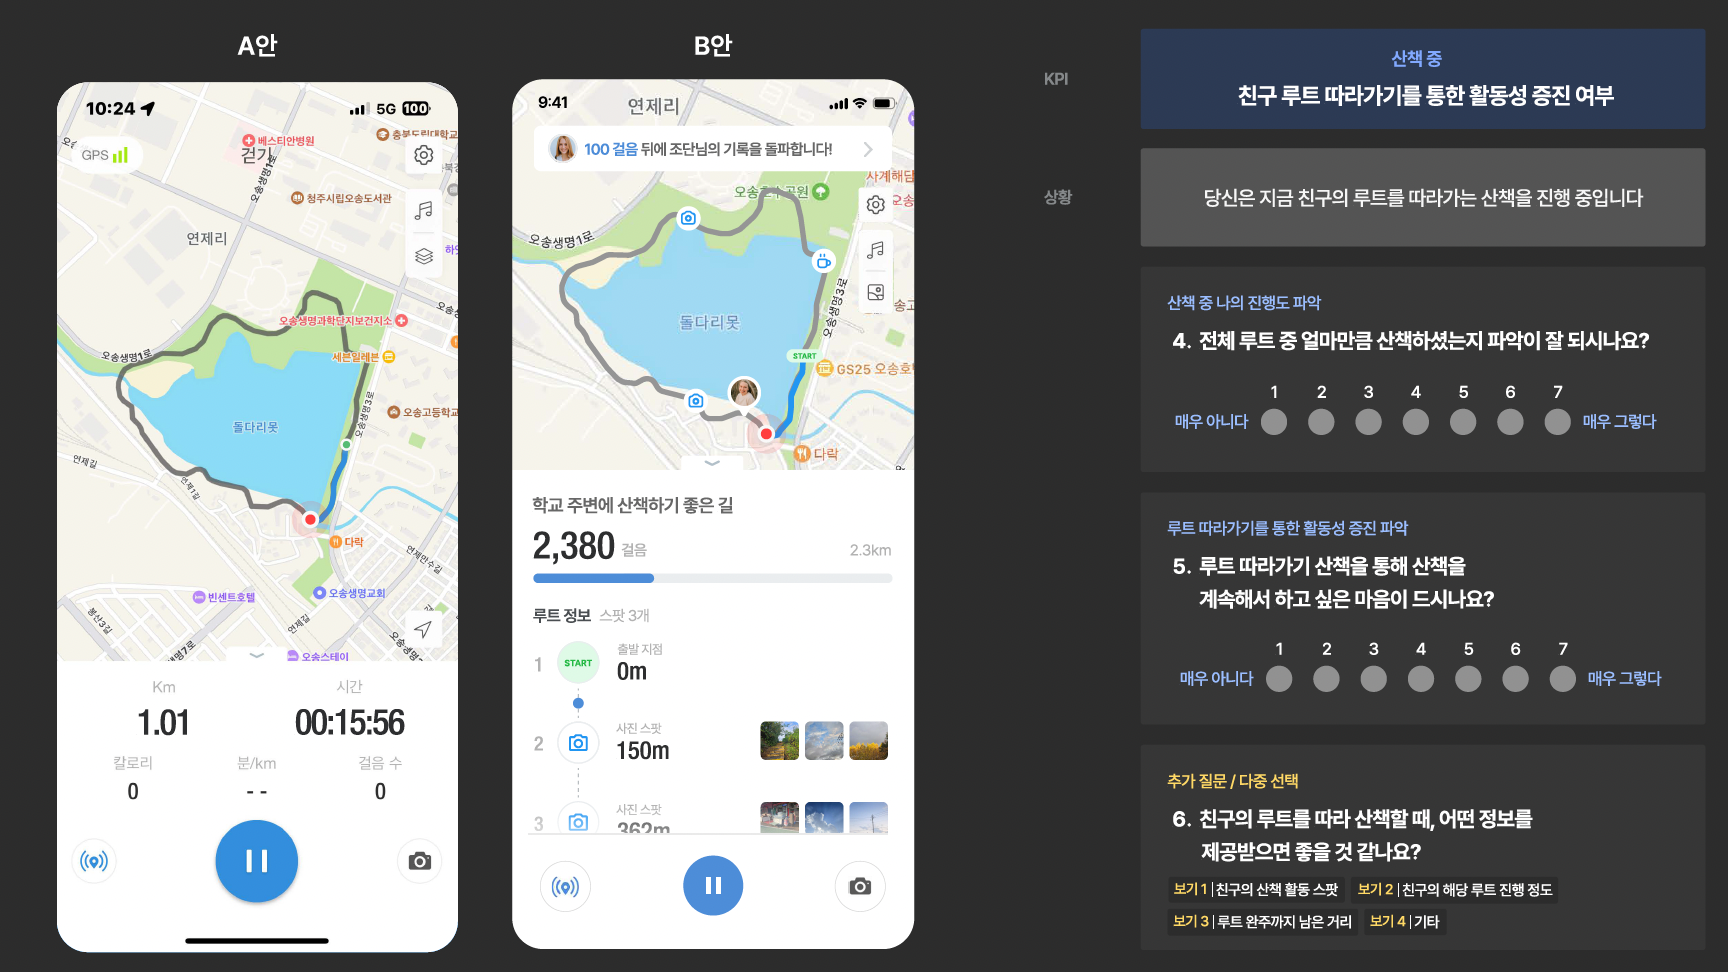
\includegraphics{img/fig30.png}

  }

  \caption{커뮤니티 기반 산책 앱의 기존 디자인(A안)과 개선 디자인(B안)의
  비교 화면과 설문 문항 예시}

  \end{figure}%
\end{enumerate}

\section{A/B 테스팅을 위한 설문 기획 Check
Point!}\label{ab-uxd14cuxc2a4uxd305uxc744-uxc704uxd55c-uxc124uxbb38-uxae30uxd68d-check-point}

\begin{itemize}
\tightlist
\item
  A안과 B안의 조사 대상 페이지 수와 콘텐츠(텍스트 원고, 이미지, 테스트
  대상이 아닌 GUI)를 동일하게 구성합니다. 아주 중요합니다. 가장
  중요합니다!!!!!
\item
  모든 원고는 사용자가 쉽게 이해할 수 있는 용어로 서술합니다. 서비스의
  전문 용어, 디자인의 전문 용어는 사용하지 않으며, 꼭 필요한 서비스
  용어는 미리 설명합니다. 디자인 평가를 하게 하는 질문은 하지 않습니다.
  우리가 측정하는 것은 KPI와 관련한 사용자 의도이지, 디자인 우수성을
  평가하는 것이 아닙니다.
\item
  질문은 존대말을 사용하고, 현재형 질문을 사용합니다. (예: 만족하시나요?
  (O), 만족하셨나요?(X)), 골라주세요---\textgreater 선택해주세요.)
\item
  서비스의 사용 상황을 설명할 필요가 있으면 그 내용도 추가하여
  설명합니다. 사용 상황에 알맞은 콘텐츠 원고를(시간, 지역, 상태 등)
  제공합니다. (예: 당신은 11월에 혼자 도쿄 여행을 준비하고 있습니다.)
\item
  설문에서는 제시하는 서비스 페이지의 이미지를 중심으로 응답을 하므로
  사용 경로(Flow) 중심의 검증은 한계가 있습니다. 화면 단위의 A/B 테스트
  방법은 사용자 경로를 검증하기에는 적합하지 않습니다.
\item
  A안에 전혀 포함되지 않은 내용이나 디자인을 질문하지 않습니다. 두 개의
  디자인에 대하여 객관적인 태도로 질문해야합니다.
\item
  설문에 제시하는 모바일 폰 테두리가 어색하지 않게 평가에 필요한
  부분으로 스크롤한 이미지를 제시합니다. (사용자가 이해하기 어려운 긴
  스크롤 뷰를 사용하지 않습니다.)
\item
  디자인 평가 대상이 아니어도 향후 디자인 개선을 위해 필요한 내용은
  객관식이나 간단한 단답식 질문으로 추가 가능합니다. (평가 내용 2의 예:
  검색 결과에 추가 되었으면하는 내용은 어떤 것인가요?) 또는 사용자의
  타겟서비스 관련 행동을 질문할 수도 있습니다. (예: 사용하는 유사
  서비스의 앱, 평소 일기쓰는 횟수 등의 질문)
\item
  사용자 구분이 필요한 경우에는 (예: heavy user와 light user의 구분)
  조건에 맞는 사용자를 미리 선정하는 스크리닝을 실시하여 같은 조건의
  사용자끼리만 비교해야합니다. 특히 A 디자인의 응답 그룹과 B 디자인의
  응답 그룹이 매우 다른 성향이라면, 결과에 영향을 미치게 됩니다. A, B
  응답자를 매우 다른 성향의 커뮤니티에서 따로 선정하거나, 나이, 성별,
  연령 등이 확연히 다른 그룹으로 테스트하면 안됩니다.
\item
  자연스러운 사용자 시나리오를 중심으로 화면 순서를 배치하고, 각 화면에
  관련한 질문(KPI 관련 질문, 추가 질문 모두)을 함께 배치합니다. 질문
  번호는 1번부터 끝번까지 이어서 사용합니다. 화면이나 질문 카테고리별로
  번호를 별도 부여하지 않습니다. 질문 섹션을 너무 많이 분리하면 설문
  시간이 길어지고, 사용자들이 불편해할 수 있습니다.
\item
  구글 설문 폼은 리커트(Likert) 문항의 디자인 자유도가 제한적이므로 폰
  화면에서 보이는 상태를 잘 고려하여 제작합니다.
\item
  설문 원고 제작과 내용 검수에 AI 서비스를 사용하는 것도 가능합니다.
  설문 목표를 제시하고, 구체적인 질문원고와 선택지를 제안하게 하거나,
  제작한 설문 원고에 문제가 없는지를 검토하도록 요청할 수 있습니다. AI를
  사용할 때는 되도록 구체적으로 상황과 목표를 설명하고, 원고의 양식이나
  예시등을 제시하여 응답의 정확도를 높이도록 합니다. 설문의 준비 과정과
  결과 분석은 AI를 사용할 수 있지만, 설문 수행을 AI로 해서는 안됩니다.
  우리는 디자인 검증을 위하여 실제 사용자의 의견을 필요로 합니다.
\end{itemize}

\chapter{ch4. A/B 테스팅 실행 및 결과의
해석}\label{ch4.-ab-uxd14cuxc2a4uxd305-uxc2e4uxd589-uxbc0f-uxacb0uxacfcuxc758-uxd574uxc11d}

\section{설문 실행}\label{uxc124uxbb38-uxc2e4uxd589}

설문지가 준비 되었으니 이제 설문을 배포하고 응답을 받습니다. 우선 설문
대상자를 정의합니다. 앞에서 설명한 것처럼 A 디자인에 대한 설문 30명
이상, B 디자인에 대한 설문 30명 이상이 참여해야하고, 두 그룹의
참여자들은 참여자로서의 조건은 동일하지만, 서로 다른 참여자입니다. 즉, A
디자인에 응답한 참여자는 B 디자인에 응답하면 안됩니다. 각 참여자가
겹치는 걸 방지하기 위해서 설문 배포 할 때도 주의 공지를 하고, 설문에
참여자의 e-mail을 받아서 동일인이 아님을 확인합니다. 참여자 e-mail
주소를 수집하면 동일인 구분에도 도움이 되지만 참여자 공지가 필요할 때나
경품 추첨 등으로 참여율을 높이고자 할 때도 유용합니다.

\begin{itemize}
\item
  본 설문을 배포하기 전에 소수 인원(2-4명)을 대상으로 파일럿
  테스트(Pilot Test)를 반드시 실시합니다.

  설문 대상자와 같은 조건의 소수 인원을 대상으로 A, B 그룹 설문 원고에
  대하여 실험을 합니다. 파일럿 테스트에서는 사용자들이 질문을 잘
  이해하는지, 의문을 가지거나 잘못 이해하는 부분은 어디인지, 응답을
  방해하거나 불편하게 하는 요인이 있는지, 응답 내용이 질문자의 의도 대로
  반영 되고 있는지를 검토합니다. 파일럿 테스트는 형식은 온라인
  설문이지만 응답자의 질문이나 상황에 바로 대응하기 위하여 대면으로
  진행하기를 권합니다. 응답자가 의문이 있을 때 바로 어떤 부분이 문제인지
  의견을 듣고, 수정안을 확인해보는 것이 좋습니다.
\item
  정확하고, 객관적인 사용자 의견을 받기 위해서 유료 설문 응답 서비스
  사용을 지양합니다.

  최근에는 설문 응답을 대행해주는 서비스들이 있어서 원하는 참여자 조건에
  맞추어 참여자들을 리크루팅하고, 설문지를 배포하고, 결과까지 분석해주는
  서비스를 사용할 수도 있습니다. 이러한 유료 대행 서비스를 사용한 사례를
  보면 사용자 응답이 긍정적 방향으로 왜곡된 현상을 발견할 수 있었습니다.
  설문 참여자들도 비용을 받고 설문에 임하는 것이기 때문에 응답률은
  높지만 전반적으로 좋은 쪽으로 응답이 기울게 되어 객관성 문제가
  발생합니다.
\item
  온라인 설문의 한계를 숙지하고 대비합니다.

  온라인 설문을 받는 것은 여러 장점이 있지만, 응답자들이 언제 응답을
  제출할지는 알 수 없습니다. 온라인 설문은 설문 요청자를 직접 만나지
  않고, 시간, 공간의 제약이 없는 것이므로, 기본적으로는 응답률이 낮은
  편입니다. 또한 설문 내용을 주의 깊게 보지 않고, 대충 답하는 응답자도
  상당수 있게 됩니다. 그래서 제공한 설문에 성의있게 답할 수 있도록
  원고의 내용이나 어투에서 정성과 신뢰감을 느끼게 하는 것이 중요합니다.
  또 응답 기한은 여유있게 잡아놓고, 초기 응답률이 낮으면, 응답률을 높일
  수 있도록 응답 대상을 넓히거나 반복해서 참여를 요청하는 등 응답 관리를
  해야합니다.
\end{itemize}

\section{설문 데이터 검수와 데이터
편집}\label{uxc124uxbb38-uxb370uxc774uxd130-uxac80uxc218uxc640-uxb370uxc774uxd130-uxd3b8uxc9d1}

우리가 진행하는 설문은 소규모이기 때문에 응답 데이터가 유효하도록
검수하는 일이 매우 중요합니다. 즉 설문 결과에 왜곡이 발생할 수 있는
성의없는 설문, 결측값이 많은 설문, 사용자 조건이 맞지 않는 설문들을
찾아서 제외할 필요가 있습니다. 그래서 설문 수가 좀 많아야 이런 문제 설문
값들을 빼고도 통계적 검증이 가능한 데이터 수를 확보할 수 있습니다.

\begin{itemize}
\tightlist
\item
  일단 리커트 척도 질문의 모든 응답이 한쪽으로 치우친 입력, 즉 모두
  1번이나 4번(중간값), 7번으로 응답한 설문이 있다면 제외합니다 .
  응답자가 성의없이 일련 번호를 입력한 경우입니다.
\item
  응답에 전반적으로 결측값이 많다면 해당 설문을 제외하는 것이 좋습니다.
  하지만 일부만 결측이 있다면, 결측 없는 응답들은 사용해도 됩니다. 이
  경우는 우리가 데이터를 분석하는 과정에서 변수 간 관계 분석이 있을
  경우에는 영향을 고려하여 신중하게 결정합니다.
\item
  응답자의 조건에 따라 응답의 내용이 큰 영향을 받는 경우는 조건을
  균일하게 맞춰야 합니다. 이전 사례를 예로 들면 결혼 준비 서비스에 대한
  설문을 하는데, 실제 결혼 준비 중인 응답자와 가상으로 결혼 준비를
  상상하고 응답하는 응답자는 응답이 매우 다를 수 있습니다. 마찬가지로
  온라인 쇼핑에서 반품 경험이 있는 사용자와 반품 경험이 없는 사용자는
  구매 태도가 다를 수 있습니다. 이렇게 설문 전에 미리 사용자 스크리닝을
  진행하지 않았는데, 응답 차이가 크게 나는 질문이 발견된 경우에는 설문
  수집 이후에라도 할 수 있으면 같은 조건의 응답으로 선별하고, 따로
  결과를 내는 것이 좋습니다. 이상과 같은 여러 상황을 대비하기 위해서는
  충분히 많을 양의 설문을 확보하는 것이 좋습니다.
\item
  설문이 완료된 데이터는 엑셀 시트로 다운로드 받아서 각 A 디자인 응답
  그룹, B 디자인 응답 그룹의 응답을 같은 질문 끼리 모아 엑셀 비교표를
  편집합니다. 2장의 {[}그림 38{]}과 같이 문항 별로 A,B 그룹의 데이터를
  배치하고, 2장의 안내와 같이 엑셀 함수를 사용하여 F-test, T-test를
  실시합니다. 주관식 문항과 A/B 테스트와 관련 없는 문항은 대응표를
  만들지 않습니다. R로 테스트 하는 경우는 A 그룹, B 그룹의 데이터를
  하나의 엑셀 표로 합친 뒤, R에서 데이터프레임으로 불러오고, 변수로 각
  그룹을 구분하여 비교하면 됩니다.
\end{itemize}

\section{F-Test, T-Test 실행과 결과
해석}\label{f-test-t-test-uxc2e4uxd589uxacfc-uxacb0uxacfc-uxd574uxc11d}

작성된 엑셀 비교 표에서 2장에서 학습한대로 각 문항 별로 F-test, T-test를
실시하고 결과 값의 p-value를 해석합니다.

\begin{itemize}
\tightlist
\item
  F-test의 결과 값이 0.05보다 크면 등분산입니다. 이후 T-test의 옵션에서
  등분산 조건을 선택합니다. 결과 값이 0.05보다 작으면 이분산입니다. 두
  그룹의 분포 정도가 다르다는 것이죠. 이 경우에는 이후 T-test의 조건을
  이분산으로 선택합니다. 데이터 비교 표에 문항 별로 등분산인지
  이분산인지 결과를 표기합니다.
\item
  T-test 함수를 계산합니다. 함수에 두 그룹에 대한 테스트 범위를
  지정하고, 양측 또는 단측 분포, 등분산 또는 이분산 옵션을 지정합니다.
  테스트 결과 값인 p-value가 0.05보다 크면 A, B 디자인에 대한 설문
  응답은 차이가 없다고 판단합니다. 반대로 0.05보다 작으로 두 값은 차이가
  있다고 판단합니다. 보통은 평균에서 두 그룹의 값이 차이가 있어도
  통계적으로는 차이가 없다는 결과가 많이 나옵니다. T-test의 판별은
  보수적인 편입니다. 엑셀 분석도구 팩을 사용하면 {[}그림 38{]}의 아래
  표와 같이 비교 데이터의 평균과 분산, 양측 및 단측 검정 값이 모두
  나오므로 분석 내용을 자세히 확인할 수 있습니다. 양측 검정 값은 단측
  검정값의 2배수입니다.
\item
  T-test는 비교적 보수적으로 판단한다고 이야기 했는데요, 예를 들어
  p-value가 0.06이 나왔다면 0.05 신뢰구간에서는 차이가 없다는
  판단이지만, 만약 신뢰 구간의 범위를 넓혀서 0.1로 한다면, 0.1보다는
  작으므로 차이가 있다고 할 수도 있습니다. 기준 값을 0.05로 잡는 것은
  통계적인 관습인데, 이를 변경하면 즉, 신뢰도를 낮추면 판정이 달라지게
  됩니다. 실험을 해보면 0.05 신뢰구간에서는 차이가 없지만 0.1
  신뢰구간에서는 차이가 있는 결과가 자주 나타납니다. 이 경우 0.1 (90\%)
  신뢰구간으로 설정했을 때는 차이가 난다고 추가적인 판정을 할 수 있으나
  결과 값의 신뢰도는 낮아지므로 주의하여 판단합니다.
\item
  이상의 방법으로 각 문항 별 A, B 디자인에 대한 응답이 차이가 있는지를
  판별하고, 문항과 연계된 KPI의 개선이 충족되었는지, 아닌지를
  판별합니다. 충족되지 않은 KPI는 왜 개선되지 않았는지를 분석해봐야
  합니다. 그리고 설문 조사의 질문 문제나 설문 참여자 선별 문제, 참여
  인원 수 문제 등 설문 조사 진행상의 문제가 있을 경우, 해당 내용과 결과
  보정 방안에 대하여 조사 방법의 한계로 서술합니다.
\end{itemize}

\section{실습과제 10: A/B 테스트 보고서
작성}\label{uxc2e4uxc2b5uxacfcuxc81c-10-ab-uxd14cuxc2a4uxd2b8-uxbcf4uxace0uxc11c-uxc791uxc131}

A/B 테스트의 실행 내용과 결과를 요약한 보고서를 작성합니다. 목차에는
다음 항목을 포함합니다. 내용을 서술할 때 테스트 과정에 대하여 전혀
모르는 사람이 봐도 이해할 수 있도록 각 단계별로 상세하고, 논리적으로
설명합니다.

\begin{itemize}
\tightlist
\item
  테스트 수행 개요 (언제, 어떤 응답자, 몇 명이, 어떻게 수행했는지를
  요약)
\item
  테스트에 사용한 A 그룹, B 그룹 설문 링크 제시
\item
  결과 요약 (각 KPI와 문항에 대하여 어떻게 결과가 나왔는지, 종합하면
  어떤 부분은 개선되고 어떤 부분은 개선되지 않았는지 요약하여 서술)
\item
  각 문항 별 제시 화면, 질문, 결과 분석 내용 정리 (질문 내용, 결과값,
  평균, F-test, T-test의 내용 및 해석)
\item
  AB 테스트의 비교 항목과 상관없는 문항에 대한 결과 요약 (사용자 프로필
  관련/ 또는 T-검정과 관련 없는 항목에 대한 데이터 시각화 및 의미 해석)
\item
  A/B 테스트의 결론 및 디자인 방향 제안(수정할 부분에 대한 컨셉), 조사
  방법론의 한계
\item
  R로 분석한 경우 html 보고서 파일로 제작해도 됩니다.
\end{itemize}

\begin{figure}[H]

{\centering 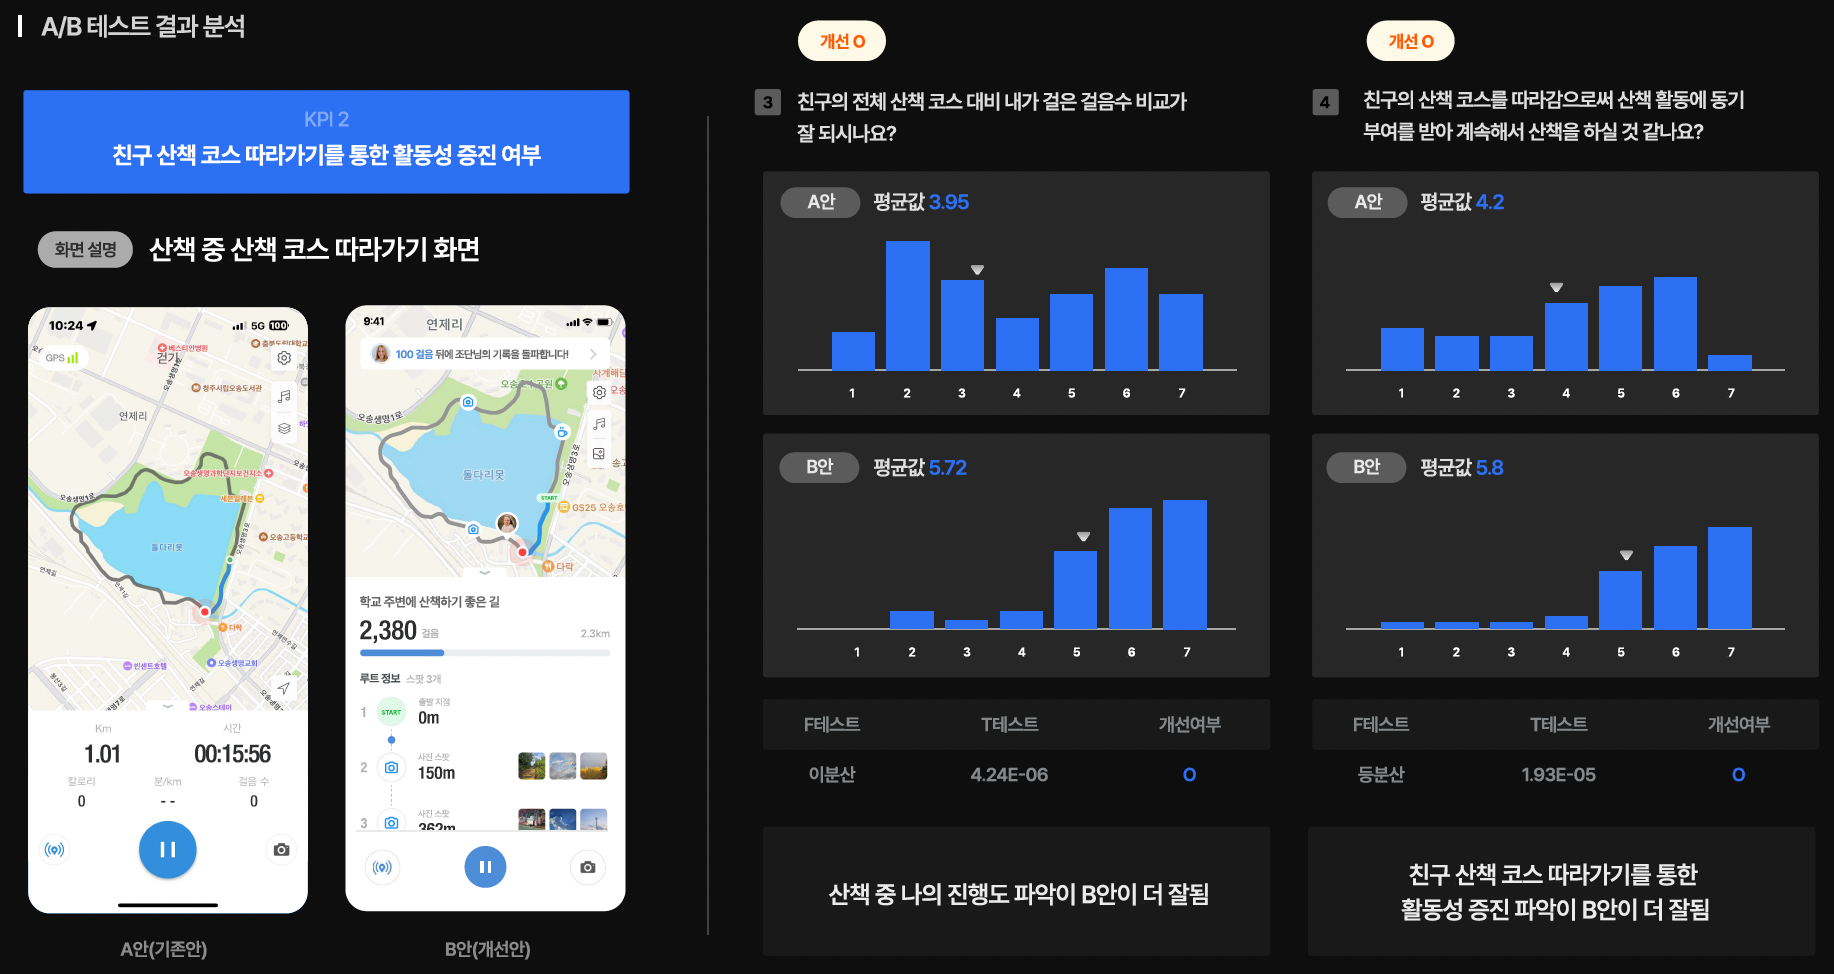
\includegraphics{img/fig31.png}

}

\caption{{[}그림 30{]}의 설문 문항에 대한 A/B 테스트 결과값 서술 예시}

\end{figure}%

\chapter{ch5. A/B 테스팅 결과의 디자인
반영}\label{ch5.-ab-uxd14cuxc2a4uxd305-uxacb0uxacfcuxc758-uxb514uxc790uxc778-uxbc18uxc601}

이제 실습 과제의 마지막 단계입니다. 우리는 실습 프로젝트에서 개선하고자
한 KPI가 개선 디자인(B안)을 통하여 개선 되었는지의 여부를 A/B 테스트로
확인했습니다. 이 결과를 어떻게 디자인에 반영해야 할까요? 다음의 사항들을
고려하여 디자인 반영 계획을 도출합니다.

\begin{itemize}
\item
  테스트에서 KPI가 개선 되었음을 확인한 B안의 디자인 개선안들은 변경
  확정을 합니다.

  다만 개선 디자인 부분들이 화면 경로의 앞, 뒤의 연계 화면에서 잘
  이어지는지, 충돌의 여지가 있는지를 확인해야합니다. 같은 개선 디자인
  요소가 반영되는 다른 화면들의 변경을 확정할 때도 다른 디자인 고려
  사항이 있는지를 확인한 후에 변경 결정을 합니다.
\item
  테스트에서 KPI가 개선 되지 않은 부분은 원인 분석을 실시하여 개선
  디자인을 수정(B' 디자인)합니다.

  응답자 리크루팅, 질문 문항의 문구, 응답 선택지 디자인 등 테스트 설계가
  잘못되었으면, 테스트를 수정하여 다시 실시해야하고, 개선 디자인에
  문제가 있었으면, 개선 디자인을 변경해야 합니다. 또는 개선 디자인은 잘
  진행 되었어도, 평가 대상이 아닌 다른 그래픽 요소 등에 영향을 받아
  문제가 생길 수도 있습니다. 예를들어, 테스트 화면에 사용한 이미지의
  크기나 이미지의 내용이 영향을 주어서 테스트 결과의 왜곡을 경험한
  사례도 있습니다. 보통 모바일 화면 레이아웃에서 눈에 띄는 이미지를
  사용하는 경우 응답자의 주의를 과도하게 분산하는 상황이 발생할 수
  있습니다. 또 설문에서 수집한 데이터 내용을 참조하여 영향을 준 원인을
  유추하는 것도 가능합니다. 이러한 원인들은 프로젝트의 성격에 따라
  다양하게 나타납니다. 명확한 원인을 찾았다면 문제를 해결하여 테스트를
  반복하면 되고, 원인이 불명확하다면 여러 가정에 따라 테스트 수정안을
  여러가지로 준비하여 하나씩 확인해나가야 합니다.
\item
  그리고 KPI에 영향을 미치지 않는 요소라고 하더라도, 서비스의 전반적인
  디자인 일관성이나 완성도 개선을 위해서, 또는 설문에서 추가적으로
  제안된 사항에 대하여도 필요성을 판단하여 디자인 개선을 진행합니다.

  여기까지 디자인 개선 계획을 확정했다면, 이상적인 서비스의 흐름을
  따라서 사용자 경험의 문제가 있는지를 검토하고, 디자인 개선을
  완료합니다. 이제 린 디자인 프로세스에 의한 UX 디자인의 한 라운드
  (Learn-Build-Measure-Learn)가 완료되었습니다.
\item
  린 디자인 프로세스는 반복적이고, 지속적인 프로세스입니다.

  기존 디자인(A 디자인)의 문제를 발견하고, KPI를 개선할 수 있는 개선
  디자인(B 디자인)을 제시하여 두 디자인의 KPI 값에 대한 개선이
  이루어졌는지를 측정하여 개선 디자인을 평가하는 한 라운드가 완료
  되었지만, 실무적 입장에서는 타겟 서비스에 대한 린 디자인 프로세스가
  이제 막 시작된 상태라고 할 수 있습니다. 이 프로세스는 목표한 KPI가
  모두 개선될 때까지 디자인 수정을 시행하면서 테스트를 반복하게 될
  것입니다. 그 외에 새로운 디자인 목표가 발생하거나, 비즈니스에 환경
  변화가 있을 때 이 과정은 새로운 라운드를 시작하게 됩니다. 이 반복적인
  개선과 검증의 순환은 서비스가 종료되는 시점까지 계속 모니터링 되고,
  지속될 것입니다.
\end{itemize}

\section{실습과제 11: 프로젝트의 최종 디자인 개선안 (디자인 B')
제시}\label{uxc2e4uxc2b5uxacfcuxc81c-11-uxd504uxb85cuxc81duxd2b8uxc758-uxcd5cuxc885-uxb514uxc790uxc778-uxac1cuxc120uxc548-uxb514uxc790uxc778-b-uxc81cuxc2dc}

A/B 테스트의 결과를 반영한 최종 디자인 개선안(디자인 B')를 제시합니다.
B' 디자인은 서비스의 실질적인 최종 디자인은 아닙니다. 새로운 디자인
개선안에 대하여 A/B 테스트를 했을 때 KPI 목표를 만족하지 못하거나 다른
디자인 문제가 발생할 수도 있고, 현 시점에서 디자인 확정이 되어도 향후에
지속적인 개선과 검증이 필요할 것이 때문입니다. 다만, 우리 실습
과제로서는 마지막 단계의 디자인 개선이므로 최종 디자인 개선안으로
표기하겠습니다.

\begin{itemize}
\tightlist
\item
  KPI가 개선 되지 않았던 화면들의 디자인에 대하여 항목 별로 원인을
  서술하고, 이를 디자인에 반영한 프로젝트의 최종 디자인 개선안(B'
  디자인) 화면을 제안합니다.
\end{itemize}

\begin{figure}[H]

{\centering 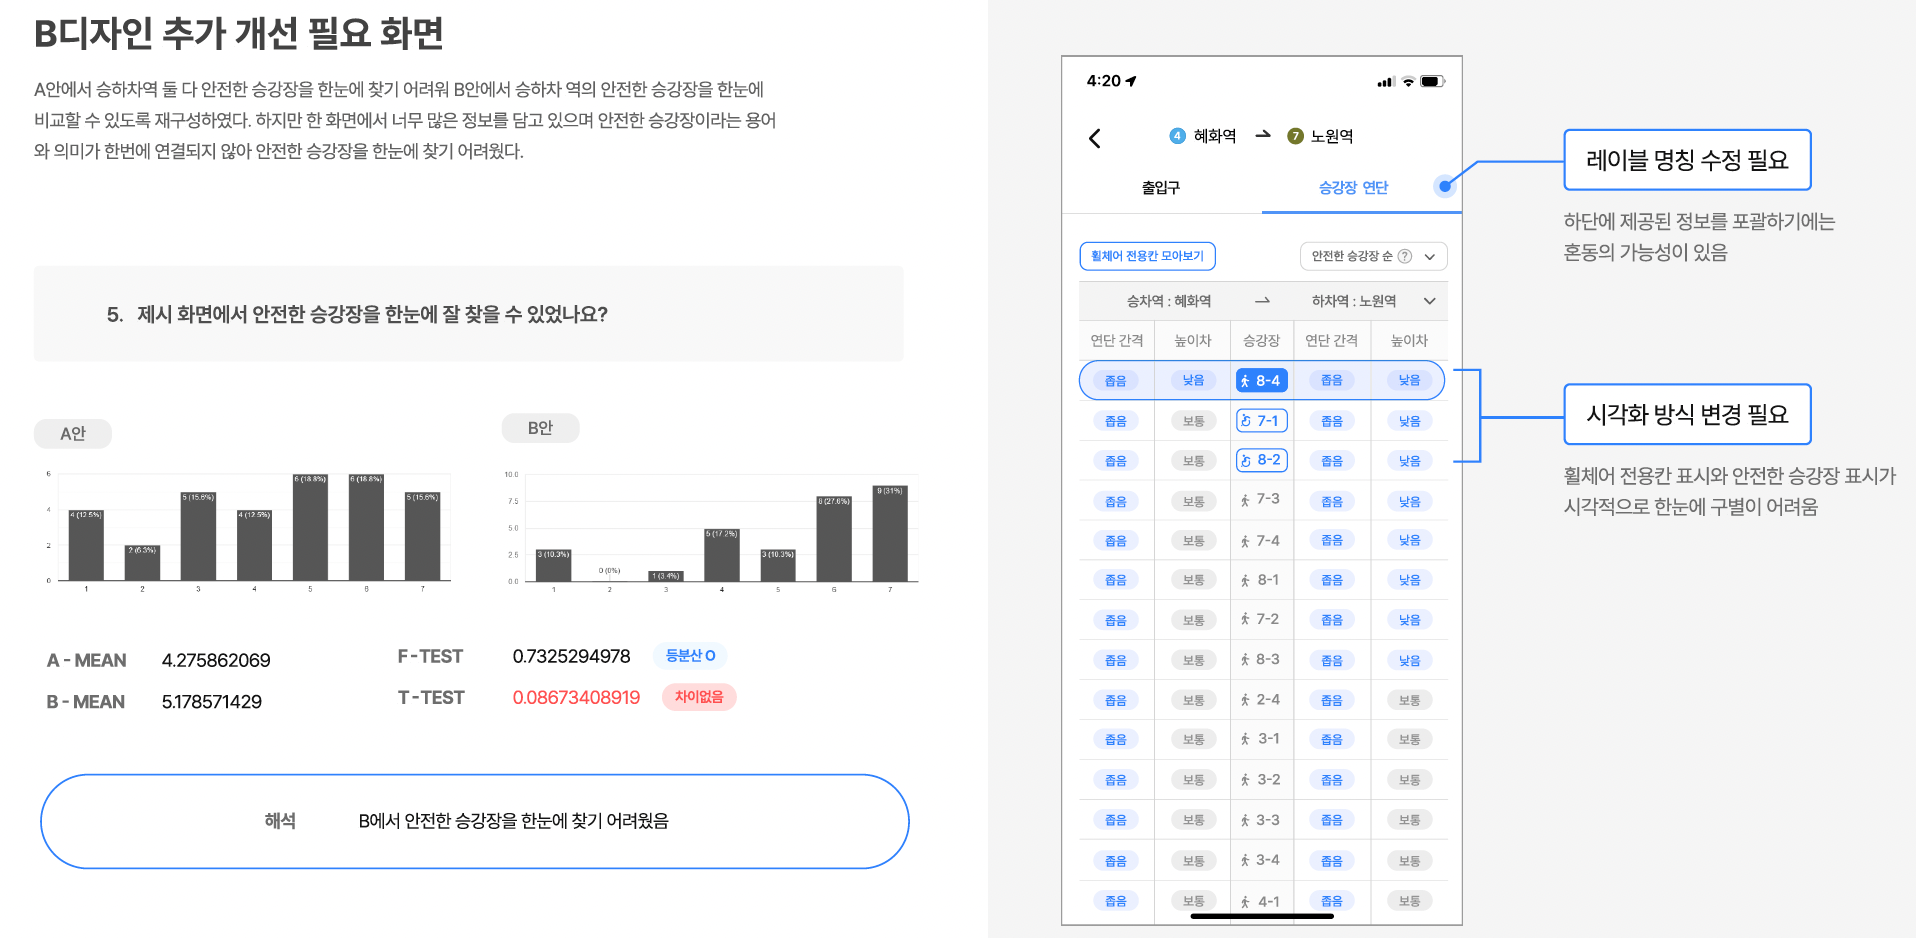
\includegraphics{img/fig32.png}

}

\caption{교통 약자를 위한 지하철 승강장 정보 화면에 대한 A/B 테스팅
결과와 B 디자인의 개선 방향 제안 예시}

\end{figure}%

\begin{itemize}
\tightlist
\item
  기존 디자인(A 디자인), 개선 디자인(B 디자인), 최종 개선 디자인(B'
  디자인)의 화면들을 서로 비교하여 변화를 이해할 수 있게 서술합니다.
\end{itemize}

\begin{figure}[H]

{\centering 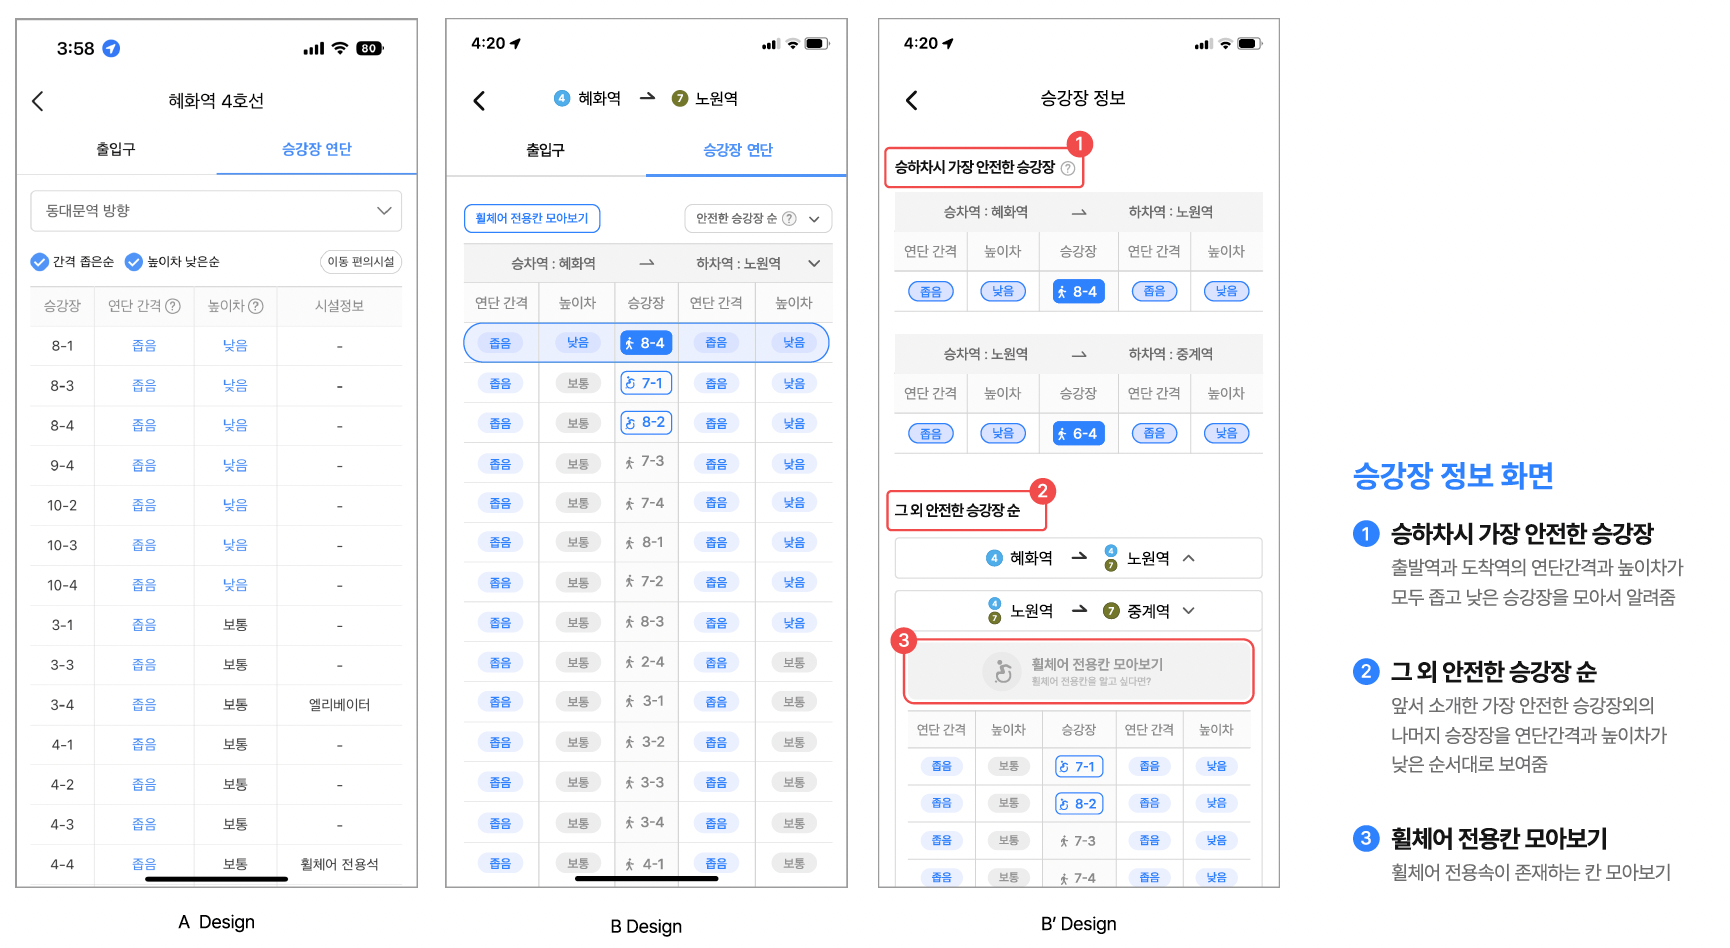
\includegraphics{img/fig33.png}

}

\caption{{[}그림 32{]}의 프로젝트에 대한 기존 디자인 A,개선 디자인 B,
최종 디자인 B' 화면의 디자인 비교 서술 예시}

\end{figure}%

\begin{itemize}
\tightlist
\item
  최종 디자인(B' 디자인)을 사용자의 사용 시나리오를 따라 제시하여 최종
  디자인의 사용자 경험을 전체적으로 이해할 수 있도록 설명합니다.
\item
  필요하다면 최종 디자인(B' 디자인)에 대한 검증 계획을 제안합니다. 이
  테스트는 이미 수행한 개선 디자인(B 디자인) 테스트의 경험과 데이터를
  활용하여 참여자, 문항, 선택지, 등의 요소들에 대한 다음 테스트 계획을
  수립합니다. 예를 들어, 진행할 테스트의 문항이 이전 테스트와 동일한
  경우에는 두번째 테스트에서 기존 디자인 (A 디자인)에 대한 평가를 새로
  하지 않고, 이미 진행한 A 디자인 데이터와 새로 수집한 B' 디자인
  데이터를 비교하여 작업 부담을 줄일 수도 있고, 기존 디자인에 대한
  설문을 추가로 시행한 뒤, 이전 설문의 데이터와 합쳐서 테스트 집단의
  규모를 크게 할 수 도 있을 것입니다. 테스트가 반복될 수록 테스트의 수행
  과정은 더 효율적으로 관리할 수 있고, 축적된 데이터들을 통하여 추가
  인사이트들을 발견할 수 있습니다.
\end{itemize}

여기까지 데이터 기반 디자인과 A/B 테스팅의 실습과제들을 마치도록
하겠습니다. 실습에 참여하시느라 수고하셨습니다.

\bookmarksetup{startatroot}

\chapter{맺음말: 다음 테스트를
위하여}\label{uxb9fauxc74cuxb9d0-uxb2e4uxc74c-uxd14cuxc2a4uxd2b8uxb97c-uxc704uxd558uxc5ec}

지금까지 데이터 기반 디자인과 Lean UX 디자인 프로세스, 디자인 검증을
위한 A/B 테스팅에 관한 이론들을 학습하고, 실습 과제들을 경험했는데요.
이제 데이터 기반 디자인에 대하여 이해가 되었다는 생각이 드시나요?

이상의 과정을 수업으로 진행하다 보면 여러가지 학생 피드백을 받게 됩니다.
가장 자주 듣는 말은 디자인하는 방법에 대한 새로운 경험을 갖게 되었다는
말입니다. 데이터 분석과 논리적 전개에 따라 시행되는 디자인은 기존에
해왔던 비교적 자유롭고, 감각적인 디자인 방법과는 차이가 있습니다. 하지만
실습 과제를 진행하면서 여전히 디자이너의 창의적 의사 결정 경로는
열려있다는 생각이 들지 않는지요? 잘 알다시피 과학이나 공학 분야도 매우
창의적인 사고가 필요합니다. 여러분이 얻은 새로운 경험을 통하여 데이터를
디자인 도구로 더 잘 사용할 수 있으면 좋겠습니다.

두번째 많이 듣는 피드백은 A/B 테스팅을 하기 위해 컨트롤 해야하는
조건들의 제약이 크다보니, 디자인 자유도가 너무 적다, 이렇게 조금씩
개선하는 것이 답답하다는 것입니다. 이것도 맞는 말이고, 이렇게 진행하면
혁신적인 디자인을 반영하기는 어려운 점이 있습니다. 그래서 이 방법은
지속적인 개선을 전제로 하는 것입니다. 린 UX 디자인 방법은 적절한 조건의
프로젝트를 만날 때 효과가 큽니다. 모든 디자인을 해결하는 방법론이
아닙니다. 그래서 A/B 테스팅 이후의 개선 디자인 수정(B' 디자인)을 실습할
때는 좀 더 자유롭고, 적극적인 디자인도 제안하도록 하여 디자이너가 느끼는
답답함을 해소하기도 합니다. 물론 린 UX의 점진적 개선 패러다임을 좀
벗어나게 되지요. 우리는 짧은 시간과 제한된 여건에서 디자인 방법을
이해하기 위한 연습을 해야하는 한계가 있음을 이해하기 바랍니다.

서술한 바와 같이 데이터 기반 디자인은 나름대로의 장점과 한계를 갖고
있습니다. 마치 디자인을 할 때 각 표현 요소마다 사용하는 툴이 달라 질 수
있듯이, 내가 디자인하는 도구에 대한 또 하나의 선택지로서 데이터 기반
디자인을 이해하면 좋겠고, 이 도구는 기존의 디자인 방법에서 아쉬웠던
특별한 지점들을 채우기 위해 개발되었다고 생각하면 좋을 듯합니다. 또
데이터 기반 디자인은 오늘날의 산업 전반에서 정말 뜨거운 주제가 되어있는
인공지능 기술과 아주 잘 융합되는 특징을 지니고 있습니다. 데이터를
이해하고, 데이터로 소통하는 능력은 디자이너가 인공지능 관련 분야에
진입할 수 있는 기본 소양이라고 할 수 있습니다. 데이터 기반 디자인 역량이
매우 필요하다는 인식은 오래전 부터 있어왔지만, 데이터 기술을 이해하고
분석하는 능력의 장애물을 넘지 못해 디자인 영역으로 편입되기
어려웠습니다. 그러나 이제는 데이터 문해력의 대중화, 데이터 분석 도구들의
발전, 인공지능 기술과의 연계 등으로 기술적인 장애물의 높이는 많이
낮아졌고, 앞으로도 점점 더 낮아지는 추세입니다. 시대적 요구와 기술
환경이 준비 되었으니, 이제는 과감하게 데이터의 장애물을 건너 디자이너의
역량을 넓혀 봅시다. 가보지 않았던 길을 가 봄으로써 우리는 새로운 세계를
발견하게 될 것입니다.

마지막으로 이 책에 담긴 다양한 디자인 사례와 실습 노하우를 축적할 수
있도록 기여해 준 우리 학부의 UX Design(2) 수업 수강생 여러분의 열린
마음과 디자인을 향한 노력에 감사를 전합니다. 그리고 뜻 깊게도 이 원고는
콘텐츠 원고를 데이터로 활용하여 web, e-bub, PDF 형태의 책으로 출판하는
R의 Quarto 서비스와 Bit Publish 소프트웨어를 사용하여 제작되었습니다.
책의 제작 과정을 통하여 데이터 기술의 또 다른 매력을 함께 경험할 수
있게되어 더욱 기쁩니다.

본 교재의 학습 경험을 바탕으로 여러분의 다음 데이터 기반 디자인
프로젝트가 성공적인 결과를 내기를 기대해보며, 원고를 마치겠습니다.

\bookmarksetup{startatroot}

\chapter*{References}\label{references}
\addcontentsline{toc}{chapter}{References}

\markboth{References}{References}

\section*{Part 1. UX 디자인과
데이터}\label{part-1.-ux-uxb514uxc790uxc778uxacfc-uxb370uxc774uxd130-2}
\addcontentsline{toc}{section}{Part 1. UX 디자인과 데이터}

\markright{Part 1. UX 디자인과 데이터}

\textbf{ch1. UX 디자인의 오늘과 변화의 방향}

(문헌1) Yvonne Rogers, Helen Sharp, Jennifer Preece, 『Interaction
Design: Beyond Human-Computer Interaction 6th edition』, Wiley. Kindle
Edition, (2023)

(문헌2) Kate Moran, Sarah Gibbons, ``Generative UI and Outcome-Oriented
Design'', \url{https://www.nngroup.com/articles/generative-ui/}, (2024)

\textbf{ch2. UX 디자인과 데이터, AI}

(문헌 3) Spotify(스포티파이), Apple app store

(문헌 4) Kate Moran, Jakob Nielsen, ``AI for UX: Getting Started'',
\url{https://www.nngroup.com/articles/ai-ux-getting-started/}, (2023)

(문헌 5) Figma Learn, ``Config 2024에서 발표된 새로운 기능'',
\url{https://help.figma.com/hc/ko/articles/24037640924823-Config-2024\%EC\%97\%90\%EC\%84\%9C-\%EB\%B0\%9C\%ED\%91\%9C\%EB\%90\%9C-\%EC\%83\%88\%EB\%A1\%9C\%EC\%9A\%B4-\%EA\%B8\%B0\%EB\%8A\%A5},
(2024)

\textbf{ch3. 데이터 기반 디자인 (Data Driven Design)}

(문헌 6) Rochelle King, Elizabeth Churchill, and Caitlin Tan,
『Designing with data』, O'reilly, (2017), pp.3-6

(문헌 7) 이현진, 『데이터 드리븐 디자인』, UX리뷰, (2024), pp.43-44

(문헌 8) Qian Yang, Alex Scuito, John Zimmerman, Jodi Forlizzi, and
Aaron Steinfeld, ``Investigating How Experienced UX Designers
Effectively Work with Machine Learning'', DIS(Design Information
Systems)(2018), Hong Kong, pp.585--596

\section*{Part 2. 디자인 리서치를 위한 탐구적 데이터
분석}\label{part-2.-uxb514uxc790uxc778-uxb9acuxc11cuxce58uxb97c-uxc704uxd55c-uxd0d0uxad6cuxc801-uxb370uxc774uxd130-uxbd84uxc11d-2}
\addcontentsline{toc}{section}{Part 2. 디자인 리서치를 위한 탐구적
데이터 분석}

\markright{Part 2. 디자인 리서치를 위한 탐구적 데이터 분석}

\textbf{ch1. 디자인 리서치와 탐구적 데이터 분석 (EDA: Exploratory Data
Analysis)}

(문헌 9) Hadley Wichham, Garrett. Grolemund, 『R for Data
Science(2e.)』, (2023), \url{https://r4ds.hadley.nz/intro}

\textbf{ch2. 디자인 리서치를 위한 탐구적 데이터 분석 사례 (1): 서울시
미세먼지 측정 데이터 분석 사례}

(문헌 7) 이현진, 『데이터 드리븐 디자인』, UX리뷰, (2024), pp.100-143

\textbf{ch3. 디자인 리서치를 위한 탐구적 데이터 분석 사례 (2):
StudentLife 데이터 분석 사례}

(문헌 10) Dartmouth College, ``StudentLife Study'', (2024.7.24),
\href{https://studentlife.cs.dartmouth.edu/}{https://studentlife.cs.dartmouth.edu}

(문헌 11) Kaggle, ``College Experience Study Dataset'', (2024.7.31)
\url{https://www.kaggle.com/datasets/subigyanepal/college-experience-dataset?resource=download}

(문헌 12) Rui Wang, et al., ''SmartGPA: How Smartphones Can Assess and
Predict Academic Performance of College Students'', UbiComp '15,
September 07-11, 2015, Osaka, Japan

(문헌 13) R. Wang et. al., ``Tracking Depression Dynamics in College
Students Using MobilePhone and Wearable Sensing'', Proceedings of the
ACM on Interactive, Mobile, Wearable and Ubiquitous Technologies, Vol.
2, No.~1, Article 43. (2018).

(문헌 14) D. L Mack, et al., ``Mental Health and Behavior of College
Students During the COVID-19 Pandemic: Longitudinal Mobile Smartphone
and Ecological Momentary Assessment Study, Part II'', JOURNAL OF MEDICAL
INTERNET RESEARCH, vol.~23, iss. 6, e28892 (2021)

(문헌 15) Subigya Nepal, et al.~``Capturing the College Experience: A
Four-Year Mobile Sensing Study of Mental Health, Resilience and Behavior
of College Students during the Pandemic.'' Proceedings of the ACM on
Interactive, Mobile, Wearable and Ubiquitous Technologies. (2024)

\textbf{ch4. EDA를 위한 데이터 분석 도구들}

(문헌 16) Google marketing platform, ``애널리틱스 기능''
\url{https://marketingplatform.google.com/intl/ko/about/analytics/features/}

(문헌 17) Microsoft, ``Power BI 둘러보기''
\url{https://powerbi.microsoft.com/ko-kr/guidedtour/power-platform/power-bi/2/1}

(문헌 18) Tableau, ``Tableau product''
\url{https://www.tableau.com/ko-kr/products/tableau}

(문헌 19) Beausable, ``Why Beausable'',
\url{https://www.beusable.net/ko/}

\textbf{ch5. Lean UX 프로세스와 데이터 기반 디자인}

(문헌 20) 로라 클라인, (김수영, 박기석 역), 『린 스타트업 실전 UX』,
한빛미디어,(2014)

(문헌 21) Google Developers, ``UXD: What is Lean UX?'',
\url{https://www.youtube.com/watch?v=7NkMm5WefBA}, (2023)

\section*{Part 3. 기존 디자인(A 디자인) 리서치와 개선 디자인(B 디자인)
제안}\label{part-3.-uxae30uxc874-uxb514uxc790uxc778a-uxb514uxc790uxc778-uxb9acuxc11cuxce58uxc640-uxac1cuxc120-uxb514uxc790uxc778b-uxb514uxc790uxc778-uxc81cuxc548-1}
\addcontentsline{toc}{section}{Part 3. 기존 디자인(A 디자인) 리서치와
개선 디자인(B 디자인) 제안}

\markright{Part 3. 기존 디자인(A 디자인) 리서치와 개선 디자인(B 디자인)
제안}

\textbf{ch1. 실습과제의 디자인 프로세스, 주제 선정}

(문헌 22) 통합 데이터지도-공공 민간 빅데이터 통합검색
\url{https://www.bigdata-map.or}

(문헌 23) MDIS 마이크로데이터 통합서비스 \url{https://mdis.kostat.go.kr}

(문헌 24) 서울 열린데이터광장 \url{https://data.seoul.go.kr}

\textbf{ch2. 데이터 큐레이션과 EDA, 디자인 인사이트}

(문헌 25) Renee. Miller, ``Big Data Curation'', 20th International
Conference on Management of Data (COMAD), (2014), p.4

(문헌 26) Google Dataset Search,
\url{https://datasetsearch.research.google.com}

\textbf{ch4. Design Concept \& MVP (Minimum Viable Product) Design}

(문헌 27) Aaron Gitlin, ``Becoming a data-aware designer'',
\url{https://uxdesign.cc/becoming-a-data-aware-designer-1d7614ebc3ed}

(문헌 28) Paperless Post, ``online invitations for all moments that
matter'', \url{https://www.paperlesspost.com}

\section*{Part 4. 개선 디자인의 검증: A/B
Testing}\label{part-4.-uxac1cuxc120-uxb514uxc790uxc778uxc758-uxac80uxc99d-ab-testing-2}
\addcontentsline{toc}{section}{Part 4. 개선 디자인의 검증: A/B Testing}

\markright{Part 4. 개선 디자인의 검증: A/B Testing}

\textbf{ch1. A/B 테스팅을 위한 기초 통계와 가설 검증 기법}

(문헌 20) 로라 클라인, (김수영, 박기석 역), 『린 스타트업 실전 UX』,
한빛미디어,(2014)

\textbf{ch2. F-test와 T-test의 실습 방법들}

(문헌 29) 구글Docs 편집기 고객센터, ``FTEST'',
\url{https://support.google.com/docs/answer/7004183?hl=ko&ref_topic=3105600}

(문헌 30) 구글Docs 편집기 고객센터, ``TTEST'',
\url{https://support.google.com/docs/answer/6055837?hl=ko}

(문헌 31) Statistics Kingdom, ``Two Sample T-Test Calculator'',
\url{https://www.statskingdom.com/140MeanT2eq.html}

(문헌 32) Statistics Kingdom, ``Shapiro-Wilk Test Calculator'',
\url{https://www.statskingdom.com/shapiro-wilk-test-calculator.html}

(문헌 33) Statistics Kingdom, ``Mann Whitney U test calculator (Wilcoxon
rank-sum)'',
\url{https://www.statskingdom.com/170median_mann_whitney.html}

(문헌 34) Emma Ding, ``A/B Testing Real-Life Example'',
\url{https://www.youtube.com/watch?v=VuKIN9S8Ivs}

\begin{center}\rule{0.5\linewidth}{0.5pt}\end{center}

\textbf{본 교재는 홍익대학교 대학혁신지원사업단의 2024년
UROP(Undergraduate Research Opportunity Program) 과제의 연구
결과물입니다.}

\textbf{(지도교수/저자: 디자인컨버전스학부 이현진, 참여학생/디자인,
제작: 디자인 컨버전스학부 이지은, 선여민)}


\backmatter
\printbibliography


\printindex


\end{document}
